% Created by tikzDevice version 0.12.3.1 on 2023-03-01 14:16:59
% !TEX encoding = UTF-8 Unicode
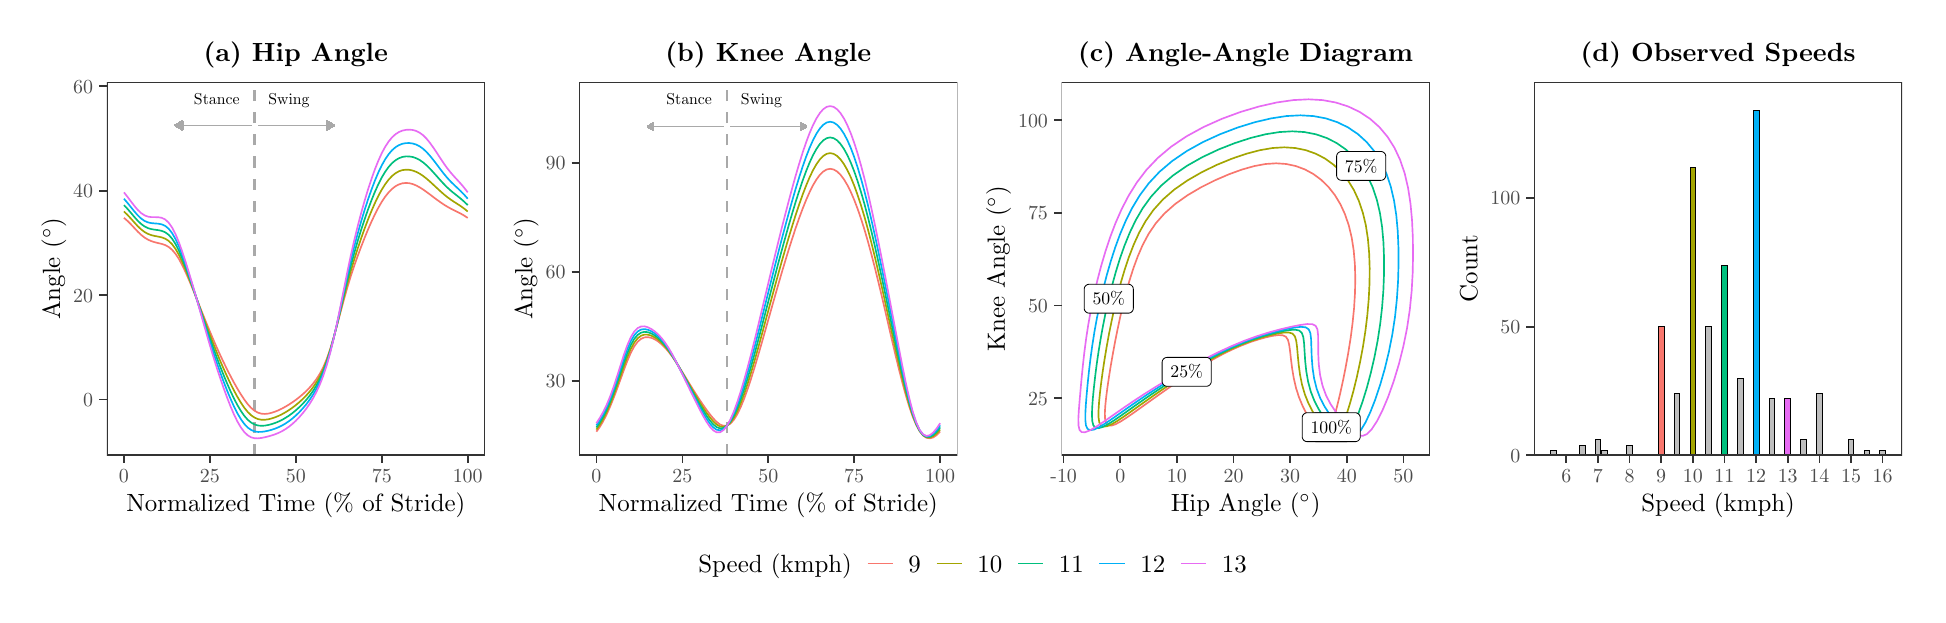
\begin{tikzpicture}[x=1pt,y=1pt]
\definecolor{fillColor}{RGB}{255,255,255}
\path[use as bounding box,fill=fillColor,fill opacity=0.00] (0,0) rectangle (682.86,204.86);
\begin{scope}
\path[clip] (  0.00, 22.44) rectangle (170.72,204.86);
\definecolor{drawColor}{RGB}{255,255,255}
\definecolor{fillColor}{RGB}{255,255,255}

\path[draw=drawColor,line width= 0.6pt,line join=round,line cap=round,fill=fillColor] ( -0.00, 22.44) rectangle (170.72,204.86);
\end{scope}
\begin{scope}
\path[clip] ( 28.58, 50.33) rectangle (165.22,185.10);
\definecolor{fillColor}{RGB}{255,255,255}

\path[fill=fillColor] ( 28.58, 50.33) rectangle (165.22,185.10);
\definecolor{drawColor}{RGB}{169,169,169}

\path[draw=drawColor,line width= 0.9pt,dash pattern=on 4pt off 4pt ,line join=round] ( 81.99, 50.33) -- ( 81.99,185.10);
\definecolor{drawColor}{RGB}{248,118,109}

\path[draw=drawColor,line width= 0.6pt,line join=round] ( 34.79,136.13) --
	( 36.04,135.06) --
	( 37.28,133.83) --
	( 38.52,132.50) --
	( 39.76,131.18) --
	( 41.01,129.98) --
	( 42.25,129.00) --
	( 43.49,128.25) --
	( 44.73,127.71) --
	( 45.97,127.32) --
	( 47.22,127.01) --
	( 48.46,126.71) --
	( 49.70,126.30) --
	( 50.94,125.63) --
	( 52.18,124.59) --
	( 53.43,123.13) --
	( 54.67,121.24) --
	( 55.91,118.94) --
	( 57.15,116.32) --
	( 58.39,113.46) --
	( 59.64,110.45) --
	( 60.88,107.37) --
	( 62.12,104.25) --
	( 63.36,101.15) --
	( 64.61, 98.08) --
	( 65.85, 95.07) --
	( 67.09, 92.14) --
	( 68.33, 89.29) --
	( 69.57, 86.55) --
	( 70.82, 83.91) --
	( 72.06, 81.37) --
	( 73.30, 78.94) --
	( 74.54, 76.62) --
	( 75.78, 74.42) --
	( 77.03, 72.36) --
	( 78.27, 70.48) --
	( 79.51, 68.83) --
	( 80.75, 67.46) --
	( 81.99, 66.43) --
	( 83.24, 65.74) --
	( 84.48, 65.37) --
	( 85.72, 65.28) --
	( 86.96, 65.41) --
	( 88.21, 65.71) --
	( 89.45, 66.12) --
	( 90.69, 66.64) --
	( 91.93, 67.24) --
	( 93.17, 67.92) --
	( 94.42, 68.67) --
	( 95.66, 69.49) --
	( 96.90, 70.37) --
	( 98.14, 71.33) --
	( 99.38, 72.37) --
	(100.63, 73.52) --
	(101.87, 74.80) --
	(103.11, 76.22) --
	(104.35, 77.87) --
	(105.59, 79.82) --
	(106.84, 82.22) --
	(108.08, 85.18) --
	(109.32, 88.75) --
	(110.56, 92.88) --
	(111.81, 97.40) --
	(113.05,102.06) --
	(114.29,106.67) --
	(115.53,111.04) --
	(116.77,115.10) --
	(118.02,118.87) --
	(119.26,122.39) --
	(120.50,125.71) --
	(121.74,128.89) --
	(122.98,131.92) --
	(124.23,134.77) --
	(125.47,137.40) --
	(126.71,139.80) --
	(127.95,141.94) --
	(129.20,143.80) --
	(130.44,145.35) --
	(131.68,146.61) --
	(132.92,147.57) --
	(134.16,148.23) --
	(135.41,148.62) --
	(136.65,148.75) --
	(137.89,148.66) --
	(139.13,148.35) --
	(140.37,147.84) --
	(141.62,147.18) --
	(142.86,146.40) --
	(144.10,145.52) --
	(145.34,144.60) --
	(146.58,143.66) --
	(147.83,142.72) --
	(149.07,141.83) --
	(150.31,140.98) --
	(151.55,140.22) --
	(152.80,139.52) --
	(154.04,138.89) --
	(155.28,138.28) --
	(156.52,137.65) --
	(157.76,136.94) --
	(159.01,136.12);
\definecolor{drawColor}{RGB}{163,165,0}

\path[draw=drawColor,line width= 0.6pt,line join=round] ( 34.79,138.43) --
	( 36.04,137.24) --
	( 37.28,135.90) --
	( 38.52,134.50) --
	( 39.76,133.14) --
	( 41.01,131.95) --
	( 42.25,131.01) --
	( 43.49,130.33) --
	( 44.73,129.88) --
	( 45.97,129.58) --
	( 47.22,129.35) --
	( 48.46,129.07) --
	( 49.70,128.61) --
	( 50.94,127.82) --
	( 52.18,126.61) --
	( 53.43,124.91) --
	( 54.67,122.74) --
	( 55.91,120.15) --
	( 57.15,117.23) --
	( 58.39,114.08) --
	( 59.64,110.79) --
	( 60.88,107.40) --
	( 62.12,103.97) --
	( 63.36,100.54) --
	( 64.61, 97.14) --
	( 65.85, 93.82) --
	( 67.09, 90.59) --
	( 68.33, 87.47) --
	( 69.57, 84.46) --
	( 70.82, 81.58) --
	( 72.06, 78.83) --
	( 73.30, 76.21) --
	( 74.54, 73.75) --
	( 75.78, 71.46) --
	( 77.03, 69.38) --
	( 78.27, 67.54) --
	( 79.51, 66.01) --
	( 80.75, 64.81) --
	( 81.99, 63.95) --
	( 83.24, 63.42) --
	( 84.48, 63.18) --
	( 85.72, 63.18) --
	( 86.96, 63.35) --
	( 88.21, 63.66) --
	( 89.45, 64.08) --
	( 90.69, 64.59) --
	( 91.93, 65.20) --
	( 93.17, 65.89) --
	( 94.42, 66.67) --
	( 95.66, 67.53) --
	( 96.90, 68.48) --
	( 98.14, 69.52) --
	( 99.38, 70.66) --
	(100.63, 71.92) --
	(101.87, 73.32) --
	(103.11, 74.90) --
	(104.35, 76.71) --
	(105.59, 78.86) --
	(106.84, 81.45) --
	(108.08, 84.62) --
	(109.32, 88.41) --
	(110.56, 92.78) --
	(111.81, 97.59) --
	(113.05,102.61) --
	(114.29,107.63) --
	(115.53,112.46) --
	(116.77,116.97) --
	(118.02,121.17) --
	(119.26,125.08) --
	(120.50,128.76) --
	(121.74,132.24) --
	(122.98,135.53) --
	(124.23,138.62) --
	(125.47,141.47) --
	(126.71,144.05) --
	(127.95,146.33) --
	(129.20,148.30) --
	(130.44,149.95) --
	(131.68,151.27) --
	(132.92,152.27) --
	(134.16,152.96) --
	(135.41,153.38) --
	(136.65,153.55) --
	(137.89,153.49) --
	(139.13,153.23) --
	(140.37,152.77) --
	(141.62,152.12) --
	(142.86,151.30) --
	(144.10,150.33) --
	(145.34,149.26) --
	(146.58,148.12) --
	(147.83,146.96) --
	(149.07,145.81) --
	(150.31,144.71) --
	(151.55,143.70) --
	(152.80,142.78) --
	(154.04,141.95) --
	(155.28,141.16) --
	(156.52,140.35) --
	(157.76,139.45) --
	(159.01,138.43);
\definecolor{drawColor}{RGB}{0,191,125}

\path[draw=drawColor,line width= 0.6pt,line join=round] ( 34.79,140.74) --
	( 36.04,139.42) --
	( 37.28,137.98) --
	( 38.52,136.50) --
	( 39.76,135.10) --
	( 41.01,133.92) --
	( 42.25,133.02) --
	( 43.49,132.41) --
	( 44.73,132.06) --
	( 45.97,131.85) --
	( 47.22,131.69) --
	( 48.46,131.43) --
	( 49.70,130.92) --
	( 50.94,130.02) --
	( 52.18,128.62) --
	( 53.43,126.69) --
	( 54.67,124.24) --
	( 55.91,121.35) --
	( 57.15,118.14) --
	( 58.39,114.71) --
	( 59.64,111.12) --
	( 60.88,107.43) --
	( 62.12,103.68) --
	( 63.36, 99.93) --
	( 64.61, 96.21) --
	( 65.85, 92.57) --
	( 67.09, 89.04) --
	( 68.33, 85.64) --
	( 69.57, 82.38) --
	( 70.82, 79.26) --
	( 72.06, 76.29) --
	( 73.30, 73.48) --
	( 74.54, 70.87) --
	( 75.78, 68.49) --
	( 77.03, 66.39) --
	( 78.27, 64.61) --
	( 79.51, 63.19) --
	( 80.75, 62.15) --
	( 81.99, 61.47) --
	( 83.24, 61.10) --
	( 84.48, 60.99) --
	( 85.72, 61.07) --
	( 86.96, 61.29) --
	( 88.21, 61.62) --
	( 89.45, 62.04) --
	( 90.69, 62.54) --
	( 91.93, 63.15) --
	( 93.17, 63.86) --
	( 94.42, 64.67) --
	( 95.66, 65.58) --
	( 96.90, 66.60) --
	( 98.14, 67.72) --
	( 99.38, 68.95) --
	(100.63, 70.32) --
	(101.87, 71.85) --
	(103.11, 73.57) --
	(104.35, 75.56) --
	(105.59, 77.89) --
	(106.84, 80.68) --
	(108.08, 84.06) --
	(109.32, 88.06) --
	(110.56, 92.68) --
	(111.81, 97.78) --
	(113.05,103.16) --
	(114.29,108.59) --
	(115.53,113.87) --
	(116.77,118.85) --
	(118.02,123.47) --
	(119.26,127.77) --
	(120.50,131.80) --
	(121.74,135.59) --
	(122.98,139.15) --
	(124.23,142.48) --
	(125.47,145.53) --
	(126.71,148.29) --
	(127.95,150.73) --
	(129.20,152.81) --
	(130.44,154.54) --
	(131.68,155.92) --
	(132.92,156.96) --
	(134.16,157.69) --
	(135.41,158.14) --
	(136.65,158.34) --
	(137.89,158.33) --
	(139.13,158.12) --
	(140.37,157.70) --
	(141.62,157.06) --
	(142.86,156.20) --
	(144.10,155.15) --
	(145.34,153.93) --
	(146.58,152.59) --
	(147.83,151.19) --
	(149.07,149.79) --
	(150.31,148.44) --
	(151.55,147.18) --
	(152.80,146.05) --
	(154.04,145.02) --
	(155.28,144.05) --
	(156.52,143.05) --
	(157.76,141.96) --
	(159.01,140.74);
\definecolor{drawColor}{RGB}{0,176,246}

\path[draw=drawColor,line width= 0.6pt,line join=round] ( 34.79,143.04) --
	( 36.04,141.59) --
	( 37.28,140.05) --
	( 38.52,138.50) --
	( 39.76,137.07) --
	( 41.01,135.88) --
	( 42.25,135.02) --
	( 43.49,134.49) --
	( 44.73,134.23) --
	( 45.97,134.12) --
	( 47.22,134.02) --
	( 48.46,133.78) --
	( 49.70,133.23) --
	( 50.94,132.22) --
	( 52.18,130.64) --
	( 53.43,128.46) --
	( 54.67,125.74) --
	( 55.91,122.56) --
	( 57.15,119.06) --
	( 58.39,115.33) --
	( 59.64,111.45) --
	( 60.88,107.46) --
	( 62.12,103.40) --
	( 63.36, 99.32) --
	( 64.61, 95.27) --
	( 65.85, 91.32) --
	( 67.09, 87.49) --
	( 68.33, 83.81) --
	( 69.57, 80.29) --
	( 70.82, 76.93) --
	( 72.06, 73.74) --
	( 73.30, 70.75) --
	( 74.54, 68.00) --
	( 75.78, 65.53) --
	( 77.03, 63.40) --
	( 78.27, 61.68) --
	( 79.51, 60.37) --
	( 80.75, 59.49) --
	( 81.99, 58.98) --
	( 83.24, 58.78) --
	( 84.48, 58.80) --
	( 85.72, 58.97) --
	( 86.96, 59.23) --
	( 88.21, 59.57) --
	( 89.45, 59.99) --
	( 90.69, 60.50) --
	( 91.93, 61.11) --
	( 93.17, 61.83) --
	( 94.42, 62.67) --
	( 95.66, 63.63) --
	( 96.90, 64.71) --
	( 98.14, 65.91) --
	( 99.38, 67.24) --
	(100.63, 68.72) --
	(101.87, 70.38) --
	(103.11, 72.25) --
	(104.35, 74.40) --
	(105.59, 76.92) --
	(106.84, 79.92) --
	(108.08, 83.50) --
	(109.32, 87.72) --
	(110.56, 92.58) --
	(111.81, 97.98) --
	(113.05,103.71) --
	(114.29,109.56) --
	(115.53,115.29) --
	(116.77,120.72) --
	(118.02,125.78) --
	(119.26,130.47) --
	(120.50,134.84) --
	(121.74,138.93) --
	(122.98,142.77) --
	(124.23,146.33) --
	(125.47,149.60) --
	(126.71,152.54) --
	(127.95,155.12) --
	(129.20,157.32) --
	(130.44,159.14) --
	(131.68,160.58) --
	(132.92,161.66) --
	(134.16,162.42) --
	(135.41,162.90) --
	(136.65,163.14) --
	(137.89,163.17) --
	(139.13,163.00) --
	(140.37,162.62) --
	(141.62,162.00) --
	(142.86,161.11) --
	(144.10,159.96) --
	(145.34,158.59) --
	(146.58,157.06) --
	(147.83,155.43) --
	(149.07,153.77) --
	(150.31,152.16) --
	(151.55,150.67) --
	(152.80,149.31) --
	(154.04,148.09) --
	(155.28,146.93) --
	(156.52,145.75) --
	(157.76,144.47) --
	(159.01,143.05);
\definecolor{drawColor}{RGB}{231,107,243}

\path[draw=drawColor,line width= 0.6pt,line join=round] ( 34.79,145.34) --
	( 36.04,143.77) --
	( 37.28,142.12) --
	( 38.52,140.50) --
	( 39.76,139.03) --
	( 41.01,137.85) --
	( 42.25,137.03) --
	( 43.49,136.57) --
	( 44.73,136.40) --
	( 45.97,136.39) --
	( 47.22,136.36) --
	( 48.46,136.14) --
	( 49.70,135.54) --
	( 50.94,134.41) --
	( 52.18,132.65) --
	( 53.43,130.24) --
	( 54.67,127.24) --
	( 55.91,123.77) --
	( 57.15,119.97) --
	( 58.39,115.95) --
	( 59.64,111.78) --
	( 60.88,107.48) --
	( 62.12,103.11) --
	( 63.36, 98.71) --
	( 64.61, 94.34) --
	( 65.85, 90.07) --
	( 67.09, 85.95) --
	( 68.33, 81.99) --
	( 69.57, 78.20) --
	( 70.82, 74.60) --
	( 72.06, 71.20) --
	( 73.30, 68.02) --
	( 74.54, 65.12) --
	( 75.78, 62.56) --
	( 77.03, 60.42) --
	( 78.27, 58.74) --
	( 79.51, 57.56) --
	( 80.75, 56.83) --
	( 81.99, 56.50) --
	( 83.24, 56.46) --
	( 84.48, 56.61) --
	( 85.72, 56.86) --
	( 86.96, 57.17) --
	( 88.21, 57.53) --
	( 89.45, 57.95) --
	( 90.69, 58.45) --
	( 91.93, 59.06) --
	( 93.17, 59.80) --
	( 94.42, 60.67) --
	( 95.66, 61.68) --
	( 96.90, 62.82) --
	( 98.14, 64.11) --
	( 99.38, 65.53) --
	(100.63, 67.12) --
	(101.87, 68.90) --
	(103.11, 70.92) --
	(104.35, 73.24) --
	(105.59, 75.95) --
	(106.84, 79.15) --
	(108.08, 82.93) --
	(109.32, 87.38) --
	(110.56, 92.48) --
	(111.81, 98.17) --
	(113.05,104.26) --
	(114.29,110.52) --
	(115.53,116.70) --
	(116.77,122.59) --
	(118.02,128.08) --
	(119.26,133.16) --
	(120.50,137.88) --
	(121.74,142.28) --
	(122.98,146.38) --
	(124.23,150.19) --
	(125.47,153.67) --
	(126.71,156.78) --
	(127.95,159.51) --
	(129.20,161.83) --
	(130.44,163.73) --
	(131.68,165.24) --
	(132.92,166.36) --
	(134.16,167.15) --
	(135.41,167.66) --
	(136.65,167.93) --
	(137.89,168.01) --
	(139.13,167.89) --
	(140.37,167.55) --
	(141.62,166.93) --
	(142.86,166.01) --
	(144.10,164.78) --
	(145.34,163.26) --
	(146.58,161.53) --
	(147.83,159.66) --
	(149.07,157.75) --
	(150.31,155.89) --
	(151.55,154.15) --
	(152.80,152.57) --
	(154.04,151.15) --
	(155.28,149.81) --
	(156.52,148.45) --
	(157.76,146.98) --
	(159.01,145.35);
\definecolor{drawColor}{RGB}{0,0,0}

\node[text=drawColor,anchor=base,inner sep=0pt, outer sep=0pt, scale=  0.57] at ( 68.33,177.01) {Stance};
\definecolor{drawColor}{RGB}{169,169,169}

\path[draw=drawColor,line width= 0.6pt,line join=round] ( 80.75,169.53) -- ( 53.43,169.53);
\definecolor{fillColor}{RGB}{169,169,169}

\path[draw=drawColor,line width= 0.6pt,line join=round,fill=fillColor] ( 55.89,170.95) --
	( 53.43,169.53) --
	( 55.89,168.11) --
	cycle;

\path[draw=drawColor,line width= 0.6pt,line join=round] ( 80.75,169.53) -- ( 53.43,169.53);

\path[draw=drawColor,line width= 0.6pt,line join=round,fill=fillColor] ( 55.89,170.95) --
	( 53.43,169.53) --
	( 55.89,168.11) --
	cycle;

\path[draw=drawColor,line width= 0.6pt,line join=round] ( 80.75,169.53) -- ( 53.43,169.53);

\path[draw=drawColor,line width= 0.6pt,line join=round,fill=fillColor] ( 55.89,170.95) --
	( 53.43,169.53) --
	( 55.89,168.11) --
	cycle;

\path[draw=drawColor,line width= 0.6pt,line join=round] ( 80.75,169.53) -- ( 53.43,169.53);

\path[draw=drawColor,line width= 0.6pt,line join=round,fill=fillColor] ( 55.89,170.95) --
	( 53.43,169.53) --
	( 55.89,168.11) --
	cycle;

\path[draw=drawColor,line width= 0.6pt,line join=round] ( 80.75,169.53) -- ( 53.43,169.53);

\path[draw=drawColor,line width= 0.6pt,line join=round,fill=fillColor] ( 55.89,170.95) --
	( 53.43,169.53) --
	( 55.89,168.11) --
	cycle;

\path[draw=drawColor,line width= 0.6pt,line join=round] ( 80.75,169.53) -- ( 53.43,169.53);

\path[draw=drawColor,line width= 0.6pt,line join=round,fill=fillColor] ( 55.89,170.95) --
	( 53.43,169.53) --
	( 55.89,168.11) --
	cycle;

\path[draw=drawColor,line width= 0.6pt,line join=round] ( 80.75,169.53) -- ( 53.43,169.53);

\path[draw=drawColor,line width= 0.6pt,line join=round,fill=fillColor] ( 55.89,170.95) --
	( 53.43,169.53) --
	( 55.89,168.11) --
	cycle;

\path[draw=drawColor,line width= 0.6pt,line join=round] ( 80.75,169.53) -- ( 53.43,169.53);

\path[draw=drawColor,line width= 0.6pt,line join=round,fill=fillColor] ( 55.89,170.95) --
	( 53.43,169.53) --
	( 55.89,168.11) --
	cycle;

\path[draw=drawColor,line width= 0.6pt,line join=round] ( 80.75,169.53) -- ( 53.43,169.53);

\path[draw=drawColor,line width= 0.6pt,line join=round,fill=fillColor] ( 55.89,170.95) --
	( 53.43,169.53) --
	( 55.89,168.11) --
	cycle;

\path[draw=drawColor,line width= 0.6pt,line join=round] ( 80.75,169.53) -- ( 53.43,169.53);

\path[draw=drawColor,line width= 0.6pt,line join=round,fill=fillColor] ( 55.89,170.95) --
	( 53.43,169.53) --
	( 55.89,168.11) --
	cycle;

\path[draw=drawColor,line width= 0.6pt,line join=round] ( 80.75,169.53) -- ( 53.43,169.53);

\path[draw=drawColor,line width= 0.6pt,line join=round,fill=fillColor] ( 55.89,170.95) --
	( 53.43,169.53) --
	( 55.89,168.11) --
	cycle;

\path[draw=drawColor,line width= 0.6pt,line join=round] ( 80.75,169.53) -- ( 53.43,169.53);

\path[draw=drawColor,line width= 0.6pt,line join=round,fill=fillColor] ( 55.89,170.95) --
	( 53.43,169.53) --
	( 55.89,168.11) --
	cycle;

\path[draw=drawColor,line width= 0.6pt,line join=round] ( 80.75,169.53) -- ( 53.43,169.53);

\path[draw=drawColor,line width= 0.6pt,line join=round,fill=fillColor] ( 55.89,170.95) --
	( 53.43,169.53) --
	( 55.89,168.11) --
	cycle;

\path[draw=drawColor,line width= 0.6pt,line join=round] ( 80.75,169.53) -- ( 53.43,169.53);

\path[draw=drawColor,line width= 0.6pt,line join=round,fill=fillColor] ( 55.89,170.95) --
	( 53.43,169.53) --
	( 55.89,168.11) --
	cycle;

\path[draw=drawColor,line width= 0.6pt,line join=round] ( 80.75,169.53) -- ( 53.43,169.53);

\path[draw=drawColor,line width= 0.6pt,line join=round,fill=fillColor] ( 55.89,170.95) --
	( 53.43,169.53) --
	( 55.89,168.11) --
	cycle;

\path[draw=drawColor,line width= 0.6pt,line join=round] ( 80.75,169.53) -- ( 53.43,169.53);

\path[draw=drawColor,line width= 0.6pt,line join=round,fill=fillColor] ( 55.89,170.95) --
	( 53.43,169.53) --
	( 55.89,168.11) --
	cycle;

\path[draw=drawColor,line width= 0.6pt,line join=round] ( 80.75,169.53) -- ( 53.43,169.53);

\path[draw=drawColor,line width= 0.6pt,line join=round,fill=fillColor] ( 55.89,170.95) --
	( 53.43,169.53) --
	( 55.89,168.11) --
	cycle;

\path[draw=drawColor,line width= 0.6pt,line join=round] ( 80.75,169.53) -- ( 53.43,169.53);

\path[draw=drawColor,line width= 0.6pt,line join=round,fill=fillColor] ( 55.89,170.95) --
	( 53.43,169.53) --
	( 55.89,168.11) --
	cycle;

\path[draw=drawColor,line width= 0.6pt,line join=round] ( 80.75,169.53) -- ( 53.43,169.53);

\path[draw=drawColor,line width= 0.6pt,line join=round,fill=fillColor] ( 55.89,170.95) --
	( 53.43,169.53) --
	( 55.89,168.11) --
	cycle;

\path[draw=drawColor,line width= 0.6pt,line join=round] ( 80.75,169.53) -- ( 53.43,169.53);

\path[draw=drawColor,line width= 0.6pt,line join=round,fill=fillColor] ( 55.89,170.95) --
	( 53.43,169.53) --
	( 55.89,168.11) --
	cycle;

\path[draw=drawColor,line width= 0.6pt,line join=round] ( 80.75,169.53) -- ( 53.43,169.53);

\path[draw=drawColor,line width= 0.6pt,line join=round,fill=fillColor] ( 55.89,170.95) --
	( 53.43,169.53) --
	( 55.89,168.11) --
	cycle;

\path[draw=drawColor,line width= 0.6pt,line join=round] ( 80.75,169.53) -- ( 53.43,169.53);

\path[draw=drawColor,line width= 0.6pt,line join=round,fill=fillColor] ( 55.89,170.95) --
	( 53.43,169.53) --
	( 55.89,168.11) --
	cycle;

\path[draw=drawColor,line width= 0.6pt,line join=round] ( 80.75,169.53) -- ( 53.43,169.53);

\path[draw=drawColor,line width= 0.6pt,line join=round,fill=fillColor] ( 55.89,170.95) --
	( 53.43,169.53) --
	( 55.89,168.11) --
	cycle;

\path[draw=drawColor,line width= 0.6pt,line join=round] ( 80.75,169.53) -- ( 53.43,169.53);

\path[draw=drawColor,line width= 0.6pt,line join=round,fill=fillColor] ( 55.89,170.95) --
	( 53.43,169.53) --
	( 55.89,168.11) --
	cycle;

\path[draw=drawColor,line width= 0.6pt,line join=round] ( 80.75,169.53) -- ( 53.43,169.53);

\path[draw=drawColor,line width= 0.6pt,line join=round,fill=fillColor] ( 55.89,170.95) --
	( 53.43,169.53) --
	( 55.89,168.11) --
	cycle;

\path[draw=drawColor,line width= 0.6pt,line join=round] ( 80.75,169.53) -- ( 53.43,169.53);

\path[draw=drawColor,line width= 0.6pt,line join=round,fill=fillColor] ( 55.89,170.95) --
	( 53.43,169.53) --
	( 55.89,168.11) --
	cycle;

\path[draw=drawColor,line width= 0.6pt,line join=round] ( 80.75,169.53) -- ( 53.43,169.53);

\path[draw=drawColor,line width= 0.6pt,line join=round,fill=fillColor] ( 55.89,170.95) --
	( 53.43,169.53) --
	( 55.89,168.11) --
	cycle;

\path[draw=drawColor,line width= 0.6pt,line join=round] ( 80.75,169.53) -- ( 53.43,169.53);

\path[draw=drawColor,line width= 0.6pt,line join=round,fill=fillColor] ( 55.89,170.95) --
	( 53.43,169.53) --
	( 55.89,168.11) --
	cycle;

\path[draw=drawColor,line width= 0.6pt,line join=round] ( 80.75,169.53) -- ( 53.43,169.53);

\path[draw=drawColor,line width= 0.6pt,line join=round,fill=fillColor] ( 55.89,170.95) --
	( 53.43,169.53) --
	( 55.89,168.11) --
	cycle;

\path[draw=drawColor,line width= 0.6pt,line join=round] ( 80.75,169.53) -- ( 53.43,169.53);

\path[draw=drawColor,line width= 0.6pt,line join=round,fill=fillColor] ( 55.89,170.95) --
	( 53.43,169.53) --
	( 55.89,168.11) --
	cycle;

\path[draw=drawColor,line width= 0.6pt,line join=round] ( 80.75,169.53) -- ( 53.43,169.53);

\path[draw=drawColor,line width= 0.6pt,line join=round,fill=fillColor] ( 55.89,170.95) --
	( 53.43,169.53) --
	( 55.89,168.11) --
	cycle;

\path[draw=drawColor,line width= 0.6pt,line join=round] ( 80.75,169.53) -- ( 53.43,169.53);

\path[draw=drawColor,line width= 0.6pt,line join=round,fill=fillColor] ( 55.89,170.95) --
	( 53.43,169.53) --
	( 55.89,168.11) --
	cycle;

\path[draw=drawColor,line width= 0.6pt,line join=round] ( 80.75,169.53) -- ( 53.43,169.53);

\path[draw=drawColor,line width= 0.6pt,line join=round,fill=fillColor] ( 55.89,170.95) --
	( 53.43,169.53) --
	( 55.89,168.11) --
	cycle;

\path[draw=drawColor,line width= 0.6pt,line join=round] ( 80.75,169.53) -- ( 53.43,169.53);

\path[draw=drawColor,line width= 0.6pt,line join=round,fill=fillColor] ( 55.89,170.95) --
	( 53.43,169.53) --
	( 55.89,168.11) --
	cycle;

\path[draw=drawColor,line width= 0.6pt,line join=round] ( 80.75,169.53) -- ( 53.43,169.53);

\path[draw=drawColor,line width= 0.6pt,line join=round,fill=fillColor] ( 55.89,170.95) --
	( 53.43,169.53) --
	( 55.89,168.11) --
	cycle;

\path[draw=drawColor,line width= 0.6pt,line join=round] ( 80.75,169.53) -- ( 53.43,169.53);

\path[draw=drawColor,line width= 0.6pt,line join=round,fill=fillColor] ( 55.89,170.95) --
	( 53.43,169.53) --
	( 55.89,168.11) --
	cycle;

\path[draw=drawColor,line width= 0.6pt,line join=round] ( 80.75,169.53) -- ( 53.43,169.53);

\path[draw=drawColor,line width= 0.6pt,line join=round,fill=fillColor] ( 55.89,170.95) --
	( 53.43,169.53) --
	( 55.89,168.11) --
	cycle;

\path[draw=drawColor,line width= 0.6pt,line join=round] ( 80.75,169.53) -- ( 53.43,169.53);

\path[draw=drawColor,line width= 0.6pt,line join=round,fill=fillColor] ( 55.89,170.95) --
	( 53.43,169.53) --
	( 55.89,168.11) --
	cycle;

\path[draw=drawColor,line width= 0.6pt,line join=round] ( 80.75,169.53) -- ( 53.43,169.53);

\path[draw=drawColor,line width= 0.6pt,line join=round,fill=fillColor] ( 55.89,170.95) --
	( 53.43,169.53) --
	( 55.89,168.11) --
	cycle;

\path[draw=drawColor,line width= 0.6pt,line join=round] ( 80.75,169.53) -- ( 53.43,169.53);

\path[draw=drawColor,line width= 0.6pt,line join=round,fill=fillColor] ( 55.89,170.95) --
	( 53.43,169.53) --
	( 55.89,168.11) --
	cycle;

\path[draw=drawColor,line width= 0.6pt,line join=round] ( 80.75,169.53) -- ( 53.43,169.53);

\path[draw=drawColor,line width= 0.6pt,line join=round,fill=fillColor] ( 55.89,170.95) --
	( 53.43,169.53) --
	( 55.89,168.11) --
	cycle;

\path[draw=drawColor,line width= 0.6pt,line join=round] ( 80.75,169.53) -- ( 53.43,169.53);

\path[draw=drawColor,line width= 0.6pt,line join=round,fill=fillColor] ( 55.89,170.95) --
	( 53.43,169.53) --
	( 55.89,168.11) --
	cycle;

\path[draw=drawColor,line width= 0.6pt,line join=round] ( 80.75,169.53) -- ( 53.43,169.53);

\path[draw=drawColor,line width= 0.6pt,line join=round,fill=fillColor] ( 55.89,170.95) --
	( 53.43,169.53) --
	( 55.89,168.11) --
	cycle;

\path[draw=drawColor,line width= 0.6pt,line join=round] ( 80.75,169.53) -- ( 53.43,169.53);

\path[draw=drawColor,line width= 0.6pt,line join=round,fill=fillColor] ( 55.89,170.95) --
	( 53.43,169.53) --
	( 55.89,168.11) --
	cycle;

\path[draw=drawColor,line width= 0.6pt,line join=round] ( 80.75,169.53) -- ( 53.43,169.53);

\path[draw=drawColor,line width= 0.6pt,line join=round,fill=fillColor] ( 55.89,170.95) --
	( 53.43,169.53) --
	( 55.89,168.11) --
	cycle;

\path[draw=drawColor,line width= 0.6pt,line join=round] ( 80.75,169.53) -- ( 53.43,169.53);

\path[draw=drawColor,line width= 0.6pt,line join=round,fill=fillColor] ( 55.89,170.95) --
	( 53.43,169.53) --
	( 55.89,168.11) --
	cycle;

\path[draw=drawColor,line width= 0.6pt,line join=round] ( 80.75,169.53) -- ( 53.43,169.53);

\path[draw=drawColor,line width= 0.6pt,line join=round,fill=fillColor] ( 55.89,170.95) --
	( 53.43,169.53) --
	( 55.89,168.11) --
	cycle;

\path[draw=drawColor,line width= 0.6pt,line join=round] ( 80.75,169.53) -- ( 53.43,169.53);

\path[draw=drawColor,line width= 0.6pt,line join=round,fill=fillColor] ( 55.89,170.95) --
	( 53.43,169.53) --
	( 55.89,168.11) --
	cycle;

\path[draw=drawColor,line width= 0.6pt,line join=round] ( 80.75,169.53) -- ( 53.43,169.53);

\path[draw=drawColor,line width= 0.6pt,line join=round,fill=fillColor] ( 55.89,170.95) --
	( 53.43,169.53) --
	( 55.89,168.11) --
	cycle;

\path[draw=drawColor,line width= 0.6pt,line join=round] ( 80.75,169.53) -- ( 53.43,169.53);

\path[draw=drawColor,line width= 0.6pt,line join=round,fill=fillColor] ( 55.89,170.95) --
	( 53.43,169.53) --
	( 55.89,168.11) --
	cycle;

\path[draw=drawColor,line width= 0.6pt,line join=round] ( 80.75,169.53) -- ( 53.43,169.53);

\path[draw=drawColor,line width= 0.6pt,line join=round,fill=fillColor] ( 55.89,170.95) --
	( 53.43,169.53) --
	( 55.89,168.11) --
	cycle;

\path[draw=drawColor,line width= 0.6pt,line join=round] ( 80.75,169.53) -- ( 53.43,169.53);

\path[draw=drawColor,line width= 0.6pt,line join=round,fill=fillColor] ( 55.89,170.95) --
	( 53.43,169.53) --
	( 55.89,168.11) --
	cycle;

\path[draw=drawColor,line width= 0.6pt,line join=round] ( 80.75,169.53) -- ( 53.43,169.53);

\path[draw=drawColor,line width= 0.6pt,line join=round,fill=fillColor] ( 55.89,170.95) --
	( 53.43,169.53) --
	( 55.89,168.11) --
	cycle;

\path[draw=drawColor,line width= 0.6pt,line join=round] ( 80.75,169.53) -- ( 53.43,169.53);

\path[draw=drawColor,line width= 0.6pt,line join=round,fill=fillColor] ( 55.89,170.95) --
	( 53.43,169.53) --
	( 55.89,168.11) --
	cycle;

\path[draw=drawColor,line width= 0.6pt,line join=round] ( 80.75,169.53) -- ( 53.43,169.53);

\path[draw=drawColor,line width= 0.6pt,line join=round,fill=fillColor] ( 55.89,170.95) --
	( 53.43,169.53) --
	( 55.89,168.11) --
	cycle;

\path[draw=drawColor,line width= 0.6pt,line join=round] ( 80.75,169.53) -- ( 53.43,169.53);

\path[draw=drawColor,line width= 0.6pt,line join=round,fill=fillColor] ( 55.89,170.95) --
	( 53.43,169.53) --
	( 55.89,168.11) --
	cycle;

\path[draw=drawColor,line width= 0.6pt,line join=round] ( 80.75,169.53) -- ( 53.43,169.53);

\path[draw=drawColor,line width= 0.6pt,line join=round,fill=fillColor] ( 55.89,170.95) --
	( 53.43,169.53) --
	( 55.89,168.11) --
	cycle;

\path[draw=drawColor,line width= 0.6pt,line join=round] ( 80.75,169.53) -- ( 53.43,169.53);

\path[draw=drawColor,line width= 0.6pt,line join=round,fill=fillColor] ( 55.89,170.95) --
	( 53.43,169.53) --
	( 55.89,168.11) --
	cycle;

\path[draw=drawColor,line width= 0.6pt,line join=round] ( 80.75,169.53) -- ( 53.43,169.53);

\path[draw=drawColor,line width= 0.6pt,line join=round,fill=fillColor] ( 55.89,170.95) --
	( 53.43,169.53) --
	( 55.89,168.11) --
	cycle;

\path[draw=drawColor,line width= 0.6pt,line join=round] ( 80.75,169.53) -- ( 53.43,169.53);

\path[draw=drawColor,line width= 0.6pt,line join=round,fill=fillColor] ( 55.89,170.95) --
	( 53.43,169.53) --
	( 55.89,168.11) --
	cycle;

\path[draw=drawColor,line width= 0.6pt,line join=round] ( 80.75,169.53) -- ( 53.43,169.53);

\path[draw=drawColor,line width= 0.6pt,line join=round,fill=fillColor] ( 55.89,170.95) --
	( 53.43,169.53) --
	( 55.89,168.11) --
	cycle;

\path[draw=drawColor,line width= 0.6pt,line join=round] ( 80.75,169.53) -- ( 53.43,169.53);

\path[draw=drawColor,line width= 0.6pt,line join=round,fill=fillColor] ( 55.89,170.95) --
	( 53.43,169.53) --
	( 55.89,168.11) --
	cycle;

\path[draw=drawColor,line width= 0.6pt,line join=round] ( 80.75,169.53) -- ( 53.43,169.53);

\path[draw=drawColor,line width= 0.6pt,line join=round,fill=fillColor] ( 55.89,170.95) --
	( 53.43,169.53) --
	( 55.89,168.11) --
	cycle;

\path[draw=drawColor,line width= 0.6pt,line join=round] ( 80.75,169.53) -- ( 53.43,169.53);

\path[draw=drawColor,line width= 0.6pt,line join=round,fill=fillColor] ( 55.89,170.95) --
	( 53.43,169.53) --
	( 55.89,168.11) --
	cycle;

\path[draw=drawColor,line width= 0.6pt,line join=round] ( 80.75,169.53) -- ( 53.43,169.53);

\path[draw=drawColor,line width= 0.6pt,line join=round,fill=fillColor] ( 55.89,170.95) --
	( 53.43,169.53) --
	( 55.89,168.11) --
	cycle;

\path[draw=drawColor,line width= 0.6pt,line join=round] ( 80.75,169.53) -- ( 53.43,169.53);

\path[draw=drawColor,line width= 0.6pt,line join=round,fill=fillColor] ( 55.89,170.95) --
	( 53.43,169.53) --
	( 55.89,168.11) --
	cycle;

\path[draw=drawColor,line width= 0.6pt,line join=round] ( 80.75,169.53) -- ( 53.43,169.53);

\path[draw=drawColor,line width= 0.6pt,line join=round,fill=fillColor] ( 55.89,170.95) --
	( 53.43,169.53) --
	( 55.89,168.11) --
	cycle;

\path[draw=drawColor,line width= 0.6pt,line join=round] ( 80.75,169.53) -- ( 53.43,169.53);

\path[draw=drawColor,line width= 0.6pt,line join=round,fill=fillColor] ( 55.89,170.95) --
	( 53.43,169.53) --
	( 55.89,168.11) --
	cycle;

\path[draw=drawColor,line width= 0.6pt,line join=round] ( 80.75,169.53) -- ( 53.43,169.53);

\path[draw=drawColor,line width= 0.6pt,line join=round,fill=fillColor] ( 55.89,170.95) --
	( 53.43,169.53) --
	( 55.89,168.11) --
	cycle;

\path[draw=drawColor,line width= 0.6pt,line join=round] ( 80.75,169.53) -- ( 53.43,169.53);

\path[draw=drawColor,line width= 0.6pt,line join=round,fill=fillColor] ( 55.89,170.95) --
	( 53.43,169.53) --
	( 55.89,168.11) --
	cycle;

\path[draw=drawColor,line width= 0.6pt,line join=round] ( 80.75,169.53) -- ( 53.43,169.53);

\path[draw=drawColor,line width= 0.6pt,line join=round,fill=fillColor] ( 55.89,170.95) --
	( 53.43,169.53) --
	( 55.89,168.11) --
	cycle;

\path[draw=drawColor,line width= 0.6pt,line join=round] ( 80.75,169.53) -- ( 53.43,169.53);

\path[draw=drawColor,line width= 0.6pt,line join=round,fill=fillColor] ( 55.89,170.95) --
	( 53.43,169.53) --
	( 55.89,168.11) --
	cycle;

\path[draw=drawColor,line width= 0.6pt,line join=round] ( 80.75,169.53) -- ( 53.43,169.53);

\path[draw=drawColor,line width= 0.6pt,line join=round,fill=fillColor] ( 55.89,170.95) --
	( 53.43,169.53) --
	( 55.89,168.11) --
	cycle;

\path[draw=drawColor,line width= 0.6pt,line join=round] ( 80.75,169.53) -- ( 53.43,169.53);

\path[draw=drawColor,line width= 0.6pt,line join=round,fill=fillColor] ( 55.89,170.95) --
	( 53.43,169.53) --
	( 55.89,168.11) --
	cycle;

\path[draw=drawColor,line width= 0.6pt,line join=round] ( 80.75,169.53) -- ( 53.43,169.53);

\path[draw=drawColor,line width= 0.6pt,line join=round,fill=fillColor] ( 55.89,170.95) --
	( 53.43,169.53) --
	( 55.89,168.11) --
	cycle;

\path[draw=drawColor,line width= 0.6pt,line join=round] ( 80.75,169.53) -- ( 53.43,169.53);

\path[draw=drawColor,line width= 0.6pt,line join=round,fill=fillColor] ( 55.89,170.95) --
	( 53.43,169.53) --
	( 55.89,168.11) --
	cycle;

\path[draw=drawColor,line width= 0.6pt,line join=round] ( 80.75,169.53) -- ( 53.43,169.53);

\path[draw=drawColor,line width= 0.6pt,line join=round,fill=fillColor] ( 55.89,170.95) --
	( 53.43,169.53) --
	( 55.89,168.11) --
	cycle;

\path[draw=drawColor,line width= 0.6pt,line join=round] ( 80.75,169.53) -- ( 53.43,169.53);

\path[draw=drawColor,line width= 0.6pt,line join=round,fill=fillColor] ( 55.89,170.95) --
	( 53.43,169.53) --
	( 55.89,168.11) --
	cycle;

\path[draw=drawColor,line width= 0.6pt,line join=round] ( 80.75,169.53) -- ( 53.43,169.53);

\path[draw=drawColor,line width= 0.6pt,line join=round,fill=fillColor] ( 55.89,170.95) --
	( 53.43,169.53) --
	( 55.89,168.11) --
	cycle;

\path[draw=drawColor,line width= 0.6pt,line join=round] ( 80.75,169.53) -- ( 53.43,169.53);

\path[draw=drawColor,line width= 0.6pt,line join=round,fill=fillColor] ( 55.89,170.95) --
	( 53.43,169.53) --
	( 55.89,168.11) --
	cycle;

\path[draw=drawColor,line width= 0.6pt,line join=round] ( 80.75,169.53) -- ( 53.43,169.53);

\path[draw=drawColor,line width= 0.6pt,line join=round,fill=fillColor] ( 55.89,170.95) --
	( 53.43,169.53) --
	( 55.89,168.11) --
	cycle;

\path[draw=drawColor,line width= 0.6pt,line join=round] ( 80.75,169.53) -- ( 53.43,169.53);

\path[draw=drawColor,line width= 0.6pt,line join=round,fill=fillColor] ( 55.89,170.95) --
	( 53.43,169.53) --
	( 55.89,168.11) --
	cycle;

\path[draw=drawColor,line width= 0.6pt,line join=round] ( 80.75,169.53) -- ( 53.43,169.53);

\path[draw=drawColor,line width= 0.6pt,line join=round,fill=fillColor] ( 55.89,170.95) --
	( 53.43,169.53) --
	( 55.89,168.11) --
	cycle;

\path[draw=drawColor,line width= 0.6pt,line join=round] ( 80.75,169.53) -- ( 53.43,169.53);

\path[draw=drawColor,line width= 0.6pt,line join=round,fill=fillColor] ( 55.89,170.95) --
	( 53.43,169.53) --
	( 55.89,168.11) --
	cycle;

\path[draw=drawColor,line width= 0.6pt,line join=round] ( 80.75,169.53) -- ( 53.43,169.53);

\path[draw=drawColor,line width= 0.6pt,line join=round,fill=fillColor] ( 55.89,170.95) --
	( 53.43,169.53) --
	( 55.89,168.11) --
	cycle;

\path[draw=drawColor,line width= 0.6pt,line join=round] ( 80.75,169.53) -- ( 53.43,169.53);

\path[draw=drawColor,line width= 0.6pt,line join=round,fill=fillColor] ( 55.89,170.95) --
	( 53.43,169.53) --
	( 55.89,168.11) --
	cycle;

\path[draw=drawColor,line width= 0.6pt,line join=round] ( 80.75,169.53) -- ( 53.43,169.53);

\path[draw=drawColor,line width= 0.6pt,line join=round,fill=fillColor] ( 55.89,170.95) --
	( 53.43,169.53) --
	( 55.89,168.11) --
	cycle;

\path[draw=drawColor,line width= 0.6pt,line join=round] ( 80.75,169.53) -- ( 53.43,169.53);

\path[draw=drawColor,line width= 0.6pt,line join=round,fill=fillColor] ( 55.89,170.95) --
	( 53.43,169.53) --
	( 55.89,168.11) --
	cycle;

\path[draw=drawColor,line width= 0.6pt,line join=round] ( 80.75,169.53) -- ( 53.43,169.53);

\path[draw=drawColor,line width= 0.6pt,line join=round,fill=fillColor] ( 55.89,170.95) --
	( 53.43,169.53) --
	( 55.89,168.11) --
	cycle;

\path[draw=drawColor,line width= 0.6pt,line join=round] ( 80.75,169.53) -- ( 53.43,169.53);

\path[draw=drawColor,line width= 0.6pt,line join=round,fill=fillColor] ( 55.89,170.95) --
	( 53.43,169.53) --
	( 55.89,168.11) --
	cycle;

\path[draw=drawColor,line width= 0.6pt,line join=round] ( 80.75,169.53) -- ( 53.43,169.53);

\path[draw=drawColor,line width= 0.6pt,line join=round,fill=fillColor] ( 55.89,170.95) --
	( 53.43,169.53) --
	( 55.89,168.11) --
	cycle;

\path[draw=drawColor,line width= 0.6pt,line join=round] ( 80.75,169.53) -- ( 53.43,169.53);

\path[draw=drawColor,line width= 0.6pt,line join=round,fill=fillColor] ( 55.89,170.95) --
	( 53.43,169.53) --
	( 55.89,168.11) --
	cycle;

\path[draw=drawColor,line width= 0.6pt,line join=round] ( 80.75,169.53) -- ( 53.43,169.53);

\path[draw=drawColor,line width= 0.6pt,line join=round,fill=fillColor] ( 55.89,170.95) --
	( 53.43,169.53) --
	( 55.89,168.11) --
	cycle;

\path[draw=drawColor,line width= 0.6pt,line join=round] ( 80.75,169.53) -- ( 53.43,169.53);

\path[draw=drawColor,line width= 0.6pt,line join=round,fill=fillColor] ( 55.89,170.95) --
	( 53.43,169.53) --
	( 55.89,168.11) --
	cycle;

\path[draw=drawColor,line width= 0.6pt,line join=round] ( 80.75,169.53) -- ( 53.43,169.53);

\path[draw=drawColor,line width= 0.6pt,line join=round,fill=fillColor] ( 55.89,170.95) --
	( 53.43,169.53) --
	( 55.89,168.11) --
	cycle;

\path[draw=drawColor,line width= 0.6pt,line join=round] ( 80.75,169.53) -- ( 53.43,169.53);

\path[draw=drawColor,line width= 0.6pt,line join=round,fill=fillColor] ( 55.89,170.95) --
	( 53.43,169.53) --
	( 55.89,168.11) --
	cycle;

\path[draw=drawColor,line width= 0.6pt,line join=round] ( 80.75,169.53) -- ( 53.43,169.53);

\path[draw=drawColor,line width= 0.6pt,line join=round,fill=fillColor] ( 55.89,170.95) --
	( 53.43,169.53) --
	( 55.89,168.11) --
	cycle;

\path[draw=drawColor,line width= 0.6pt,line join=round] ( 80.75,169.53) -- ( 53.43,169.53);

\path[draw=drawColor,line width= 0.6pt,line join=round,fill=fillColor] ( 55.89,170.95) --
	( 53.43,169.53) --
	( 55.89,168.11) --
	cycle;

\path[draw=drawColor,line width= 0.6pt,line join=round] ( 80.75,169.53) -- ( 53.43,169.53);

\path[draw=drawColor,line width= 0.6pt,line join=round,fill=fillColor] ( 55.89,170.95) --
	( 53.43,169.53) --
	( 55.89,168.11) --
	cycle;

\path[draw=drawColor,line width= 0.6pt,line join=round] ( 80.75,169.53) -- ( 53.43,169.53);

\path[draw=drawColor,line width= 0.6pt,line join=round,fill=fillColor] ( 55.89,170.95) --
	( 53.43,169.53) --
	( 55.89,168.11) --
	cycle;

\path[draw=drawColor,line width= 0.6pt,line join=round] ( 80.75,169.53) -- ( 53.43,169.53);

\path[draw=drawColor,line width= 0.6pt,line join=round,fill=fillColor] ( 55.89,170.95) --
	( 53.43,169.53) --
	( 55.89,168.11) --
	cycle;

\path[draw=drawColor,line width= 0.6pt,line join=round] ( 80.75,169.53) -- ( 53.43,169.53);

\path[draw=drawColor,line width= 0.6pt,line join=round,fill=fillColor] ( 55.89,170.95) --
	( 53.43,169.53) --
	( 55.89,168.11) --
	cycle;

\path[draw=drawColor,line width= 0.6pt,line join=round] ( 80.75,169.53) -- ( 53.43,169.53);

\path[draw=drawColor,line width= 0.6pt,line join=round,fill=fillColor] ( 55.89,170.95) --
	( 53.43,169.53) --
	( 55.89,168.11) --
	cycle;

\path[draw=drawColor,line width= 0.6pt,line join=round] ( 80.75,169.53) -- ( 53.43,169.53);

\path[draw=drawColor,line width= 0.6pt,line join=round,fill=fillColor] ( 55.89,170.95) --
	( 53.43,169.53) --
	( 55.89,168.11) --
	cycle;

\path[draw=drawColor,line width= 0.6pt,line join=round] ( 80.75,169.53) -- ( 53.43,169.53);

\path[draw=drawColor,line width= 0.6pt,line join=round,fill=fillColor] ( 55.89,170.95) --
	( 53.43,169.53) --
	( 55.89,168.11) --
	cycle;

\path[draw=drawColor,line width= 0.6pt,line join=round] ( 80.75,169.53) -- ( 53.43,169.53);

\path[draw=drawColor,line width= 0.6pt,line join=round,fill=fillColor] ( 55.89,170.95) --
	( 53.43,169.53) --
	( 55.89,168.11) --
	cycle;

\path[draw=drawColor,line width= 0.6pt,line join=round] ( 80.75,169.53) -- ( 53.43,169.53);

\path[draw=drawColor,line width= 0.6pt,line join=round,fill=fillColor] ( 55.89,170.95) --
	( 53.43,169.53) --
	( 55.89,168.11) --
	cycle;

\path[draw=drawColor,line width= 0.6pt,line join=round] ( 80.75,169.53) -- ( 53.43,169.53);

\path[draw=drawColor,line width= 0.6pt,line join=round,fill=fillColor] ( 55.89,170.95) --
	( 53.43,169.53) --
	( 55.89,168.11) --
	cycle;

\path[draw=drawColor,line width= 0.6pt,line join=round] ( 80.75,169.53) -- ( 53.43,169.53);

\path[draw=drawColor,line width= 0.6pt,line join=round,fill=fillColor] ( 55.89,170.95) --
	( 53.43,169.53) --
	( 55.89,168.11) --
	cycle;

\path[draw=drawColor,line width= 0.6pt,line join=round] ( 80.75,169.53) -- ( 53.43,169.53);

\path[draw=drawColor,line width= 0.6pt,line join=round,fill=fillColor] ( 55.89,170.95) --
	( 53.43,169.53) --
	( 55.89,168.11) --
	cycle;

\path[draw=drawColor,line width= 0.6pt,line join=round] ( 80.75,169.53) -- ( 53.43,169.53);

\path[draw=drawColor,line width= 0.6pt,line join=round,fill=fillColor] ( 55.89,170.95) --
	( 53.43,169.53) --
	( 55.89,168.11) --
	cycle;

\path[draw=drawColor,line width= 0.6pt,line join=round] ( 80.75,169.53) -- ( 53.43,169.53);

\path[draw=drawColor,line width= 0.6pt,line join=round,fill=fillColor] ( 55.89,170.95) --
	( 53.43,169.53) --
	( 55.89,168.11) --
	cycle;

\path[draw=drawColor,line width= 0.6pt,line join=round] ( 80.75,169.53) -- ( 53.43,169.53);

\path[draw=drawColor,line width= 0.6pt,line join=round,fill=fillColor] ( 55.89,170.95) --
	( 53.43,169.53) --
	( 55.89,168.11) --
	cycle;

\path[draw=drawColor,line width= 0.6pt,line join=round] ( 80.75,169.53) -- ( 53.43,169.53);

\path[draw=drawColor,line width= 0.6pt,line join=round,fill=fillColor] ( 55.89,170.95) --
	( 53.43,169.53) --
	( 55.89,168.11) --
	cycle;

\path[draw=drawColor,line width= 0.6pt,line join=round] ( 80.75,169.53) -- ( 53.43,169.53);

\path[draw=drawColor,line width= 0.6pt,line join=round,fill=fillColor] ( 55.89,170.95) --
	( 53.43,169.53) --
	( 55.89,168.11) --
	cycle;

\path[draw=drawColor,line width= 0.6pt,line join=round] ( 80.75,169.53) -- ( 53.43,169.53);

\path[draw=drawColor,line width= 0.6pt,line join=round,fill=fillColor] ( 55.89,170.95) --
	( 53.43,169.53) --
	( 55.89,168.11) --
	cycle;

\path[draw=drawColor,line width= 0.6pt,line join=round] ( 80.75,169.53) -- ( 53.43,169.53);

\path[draw=drawColor,line width= 0.6pt,line join=round,fill=fillColor] ( 55.89,170.95) --
	( 53.43,169.53) --
	( 55.89,168.11) --
	cycle;

\path[draw=drawColor,line width= 0.6pt,line join=round] ( 80.75,169.53) -- ( 53.43,169.53);

\path[draw=drawColor,line width= 0.6pt,line join=round,fill=fillColor] ( 55.89,170.95) --
	( 53.43,169.53) --
	( 55.89,168.11) --
	cycle;

\path[draw=drawColor,line width= 0.6pt,line join=round] ( 80.75,169.53) -- ( 53.43,169.53);

\path[draw=drawColor,line width= 0.6pt,line join=round,fill=fillColor] ( 55.89,170.95) --
	( 53.43,169.53) --
	( 55.89,168.11) --
	cycle;

\path[draw=drawColor,line width= 0.6pt,line join=round] ( 80.75,169.53) -- ( 53.43,169.53);

\path[draw=drawColor,line width= 0.6pt,line join=round,fill=fillColor] ( 55.89,170.95) --
	( 53.43,169.53) --
	( 55.89,168.11) --
	cycle;

\path[draw=drawColor,line width= 0.6pt,line join=round] ( 80.75,169.53) -- ( 53.43,169.53);

\path[draw=drawColor,line width= 0.6pt,line join=round,fill=fillColor] ( 55.89,170.95) --
	( 53.43,169.53) --
	( 55.89,168.11) --
	cycle;

\path[draw=drawColor,line width= 0.6pt,line join=round] ( 80.75,169.53) -- ( 53.43,169.53);

\path[draw=drawColor,line width= 0.6pt,line join=round,fill=fillColor] ( 55.89,170.95) --
	( 53.43,169.53) --
	( 55.89,168.11) --
	cycle;

\path[draw=drawColor,line width= 0.6pt,line join=round] ( 80.75,169.53) -- ( 53.43,169.53);

\path[draw=drawColor,line width= 0.6pt,line join=round,fill=fillColor] ( 55.89,170.95) --
	( 53.43,169.53) --
	( 55.89,168.11) --
	cycle;

\path[draw=drawColor,line width= 0.6pt,line join=round] ( 80.75,169.53) -- ( 53.43,169.53);

\path[draw=drawColor,line width= 0.6pt,line join=round,fill=fillColor] ( 55.89,170.95) --
	( 53.43,169.53) --
	( 55.89,168.11) --
	cycle;

\path[draw=drawColor,line width= 0.6pt,line join=round] ( 80.75,169.53) -- ( 53.43,169.53);

\path[draw=drawColor,line width= 0.6pt,line join=round,fill=fillColor] ( 55.89,170.95) --
	( 53.43,169.53) --
	( 55.89,168.11) --
	cycle;

\path[draw=drawColor,line width= 0.6pt,line join=round] ( 80.75,169.53) -- ( 53.43,169.53);

\path[draw=drawColor,line width= 0.6pt,line join=round,fill=fillColor] ( 55.89,170.95) --
	( 53.43,169.53) --
	( 55.89,168.11) --
	cycle;

\path[draw=drawColor,line width= 0.6pt,line join=round] ( 80.75,169.53) -- ( 53.43,169.53);

\path[draw=drawColor,line width= 0.6pt,line join=round,fill=fillColor] ( 55.89,170.95) --
	( 53.43,169.53) --
	( 55.89,168.11) --
	cycle;

\path[draw=drawColor,line width= 0.6pt,line join=round] ( 80.75,169.53) -- ( 53.43,169.53);

\path[draw=drawColor,line width= 0.6pt,line join=round,fill=fillColor] ( 55.89,170.95) --
	( 53.43,169.53) --
	( 55.89,168.11) --
	cycle;

\path[draw=drawColor,line width= 0.6pt,line join=round] ( 80.75,169.53) -- ( 53.43,169.53);

\path[draw=drawColor,line width= 0.6pt,line join=round,fill=fillColor] ( 55.89,170.95) --
	( 53.43,169.53) --
	( 55.89,168.11) --
	cycle;

\path[draw=drawColor,line width= 0.6pt,line join=round] ( 80.75,169.53) -- ( 53.43,169.53);

\path[draw=drawColor,line width= 0.6pt,line join=round,fill=fillColor] ( 55.89,170.95) --
	( 53.43,169.53) --
	( 55.89,168.11) --
	cycle;

\path[draw=drawColor,line width= 0.6pt,line join=round] ( 80.75,169.53) -- ( 53.43,169.53);

\path[draw=drawColor,line width= 0.6pt,line join=round,fill=fillColor] ( 55.89,170.95) --
	( 53.43,169.53) --
	( 55.89,168.11) --
	cycle;

\path[draw=drawColor,line width= 0.6pt,line join=round] ( 80.75,169.53) -- ( 53.43,169.53);

\path[draw=drawColor,line width= 0.6pt,line join=round,fill=fillColor] ( 55.89,170.95) --
	( 53.43,169.53) --
	( 55.89,168.11) --
	cycle;

\path[draw=drawColor,line width= 0.6pt,line join=round] ( 80.75,169.53) -- ( 53.43,169.53);

\path[draw=drawColor,line width= 0.6pt,line join=round,fill=fillColor] ( 55.89,170.95) --
	( 53.43,169.53) --
	( 55.89,168.11) --
	cycle;

\path[draw=drawColor,line width= 0.6pt,line join=round] ( 80.75,169.53) -- ( 53.43,169.53);

\path[draw=drawColor,line width= 0.6pt,line join=round,fill=fillColor] ( 55.89,170.95) --
	( 53.43,169.53) --
	( 55.89,168.11) --
	cycle;

\path[draw=drawColor,line width= 0.6pt,line join=round] ( 80.75,169.53) -- ( 53.43,169.53);

\path[draw=drawColor,line width= 0.6pt,line join=round,fill=fillColor] ( 55.89,170.95) --
	( 53.43,169.53) --
	( 55.89,168.11) --
	cycle;

\path[draw=drawColor,line width= 0.6pt,line join=round] ( 80.75,169.53) -- ( 53.43,169.53);

\path[draw=drawColor,line width= 0.6pt,line join=round,fill=fillColor] ( 55.89,170.95) --
	( 53.43,169.53) --
	( 55.89,168.11) --
	cycle;

\path[draw=drawColor,line width= 0.6pt,line join=round] ( 80.75,169.53) -- ( 53.43,169.53);

\path[draw=drawColor,line width= 0.6pt,line join=round,fill=fillColor] ( 55.89,170.95) --
	( 53.43,169.53) --
	( 55.89,168.11) --
	cycle;

\path[draw=drawColor,line width= 0.6pt,line join=round] ( 80.75,169.53) -- ( 53.43,169.53);

\path[draw=drawColor,line width= 0.6pt,line join=round,fill=fillColor] ( 55.89,170.95) --
	( 53.43,169.53) --
	( 55.89,168.11) --
	cycle;

\path[draw=drawColor,line width= 0.6pt,line join=round] ( 80.75,169.53) -- ( 53.43,169.53);

\path[draw=drawColor,line width= 0.6pt,line join=round,fill=fillColor] ( 55.89,170.95) --
	( 53.43,169.53) --
	( 55.89,168.11) --
	cycle;

\path[draw=drawColor,line width= 0.6pt,line join=round] ( 80.75,169.53) -- ( 53.43,169.53);

\path[draw=drawColor,line width= 0.6pt,line join=round,fill=fillColor] ( 55.89,170.95) --
	( 53.43,169.53) --
	( 55.89,168.11) --
	cycle;

\path[draw=drawColor,line width= 0.6pt,line join=round] ( 80.75,169.53) -- ( 53.43,169.53);

\path[draw=drawColor,line width= 0.6pt,line join=round,fill=fillColor] ( 55.89,170.95) --
	( 53.43,169.53) --
	( 55.89,168.11) --
	cycle;

\path[draw=drawColor,line width= 0.6pt,line join=round] ( 80.75,169.53) -- ( 53.43,169.53);

\path[draw=drawColor,line width= 0.6pt,line join=round,fill=fillColor] ( 55.89,170.95) --
	( 53.43,169.53) --
	( 55.89,168.11) --
	cycle;

\path[draw=drawColor,line width= 0.6pt,line join=round] ( 80.75,169.53) -- ( 53.43,169.53);

\path[draw=drawColor,line width= 0.6pt,line join=round,fill=fillColor] ( 55.89,170.95) --
	( 53.43,169.53) --
	( 55.89,168.11) --
	cycle;

\path[draw=drawColor,line width= 0.6pt,line join=round] ( 80.75,169.53) -- ( 53.43,169.53);

\path[draw=drawColor,line width= 0.6pt,line join=round,fill=fillColor] ( 55.89,170.95) --
	( 53.43,169.53) --
	( 55.89,168.11) --
	cycle;

\path[draw=drawColor,line width= 0.6pt,line join=round] ( 80.75,169.53) -- ( 53.43,169.53);

\path[draw=drawColor,line width= 0.6pt,line join=round,fill=fillColor] ( 55.89,170.95) --
	( 53.43,169.53) --
	( 55.89,168.11) --
	cycle;

\path[draw=drawColor,line width= 0.6pt,line join=round] ( 80.75,169.53) -- ( 53.43,169.53);

\path[draw=drawColor,line width= 0.6pt,line join=round,fill=fillColor] ( 55.89,170.95) --
	( 53.43,169.53) --
	( 55.89,168.11) --
	cycle;

\path[draw=drawColor,line width= 0.6pt,line join=round] ( 80.75,169.53) -- ( 53.43,169.53);

\path[draw=drawColor,line width= 0.6pt,line join=round,fill=fillColor] ( 55.89,170.95) --
	( 53.43,169.53) --
	( 55.89,168.11) --
	cycle;

\path[draw=drawColor,line width= 0.6pt,line join=round] ( 80.75,169.53) -- ( 53.43,169.53);

\path[draw=drawColor,line width= 0.6pt,line join=round,fill=fillColor] ( 55.89,170.95) --
	( 53.43,169.53) --
	( 55.89,168.11) --
	cycle;

\path[draw=drawColor,line width= 0.6pt,line join=round] ( 80.75,169.53) -- ( 53.43,169.53);

\path[draw=drawColor,line width= 0.6pt,line join=round,fill=fillColor] ( 55.89,170.95) --
	( 53.43,169.53) --
	( 55.89,168.11) --
	cycle;

\path[draw=drawColor,line width= 0.6pt,line join=round] ( 80.75,169.53) -- ( 53.43,169.53);

\path[draw=drawColor,line width= 0.6pt,line join=round,fill=fillColor] ( 55.89,170.95) --
	( 53.43,169.53) --
	( 55.89,168.11) --
	cycle;

\path[draw=drawColor,line width= 0.6pt,line join=round] ( 80.75,169.53) -- ( 53.43,169.53);

\path[draw=drawColor,line width= 0.6pt,line join=round,fill=fillColor] ( 55.89,170.95) --
	( 53.43,169.53) --
	( 55.89,168.11) --
	cycle;

\path[draw=drawColor,line width= 0.6pt,line join=round] ( 80.75,169.53) -- ( 53.43,169.53);

\path[draw=drawColor,line width= 0.6pt,line join=round,fill=fillColor] ( 55.89,170.95) --
	( 53.43,169.53) --
	( 55.89,168.11) --
	cycle;

\path[draw=drawColor,line width= 0.6pt,line join=round] ( 80.75,169.53) -- ( 53.43,169.53);

\path[draw=drawColor,line width= 0.6pt,line join=round,fill=fillColor] ( 55.89,170.95) --
	( 53.43,169.53) --
	( 55.89,168.11) --
	cycle;

\path[draw=drawColor,line width= 0.6pt,line join=round] ( 80.75,169.53) -- ( 53.43,169.53);

\path[draw=drawColor,line width= 0.6pt,line join=round,fill=fillColor] ( 55.89,170.95) --
	( 53.43,169.53) --
	( 55.89,168.11) --
	cycle;

\path[draw=drawColor,line width= 0.6pt,line join=round] ( 80.75,169.53) -- ( 53.43,169.53);

\path[draw=drawColor,line width= 0.6pt,line join=round,fill=fillColor] ( 55.89,170.95) --
	( 53.43,169.53) --
	( 55.89,168.11) --
	cycle;

\path[draw=drawColor,line width= 0.6pt,line join=round] ( 80.75,169.53) -- ( 53.43,169.53);

\path[draw=drawColor,line width= 0.6pt,line join=round,fill=fillColor] ( 55.89,170.95) --
	( 53.43,169.53) --
	( 55.89,168.11) --
	cycle;

\path[draw=drawColor,line width= 0.6pt,line join=round] ( 80.75,169.53) -- ( 53.43,169.53);

\path[draw=drawColor,line width= 0.6pt,line join=round,fill=fillColor] ( 55.89,170.95) --
	( 53.43,169.53) --
	( 55.89,168.11) --
	cycle;

\path[draw=drawColor,line width= 0.6pt,line join=round] ( 80.75,169.53) -- ( 53.43,169.53);

\path[draw=drawColor,line width= 0.6pt,line join=round,fill=fillColor] ( 55.89,170.95) --
	( 53.43,169.53) --
	( 55.89,168.11) --
	cycle;

\path[draw=drawColor,line width= 0.6pt,line join=round] ( 80.75,169.53) -- ( 53.43,169.53);

\path[draw=drawColor,line width= 0.6pt,line join=round,fill=fillColor] ( 55.89,170.95) --
	( 53.43,169.53) --
	( 55.89,168.11) --
	cycle;

\path[draw=drawColor,line width= 0.6pt,line join=round] ( 80.75,169.53) -- ( 53.43,169.53);

\path[draw=drawColor,line width= 0.6pt,line join=round,fill=fillColor] ( 55.89,170.95) --
	( 53.43,169.53) --
	( 55.89,168.11) --
	cycle;

\path[draw=drawColor,line width= 0.6pt,line join=round] ( 80.75,169.53) -- ( 53.43,169.53);

\path[draw=drawColor,line width= 0.6pt,line join=round,fill=fillColor] ( 55.89,170.95) --
	( 53.43,169.53) --
	( 55.89,168.11) --
	cycle;

\path[draw=drawColor,line width= 0.6pt,line join=round] ( 80.75,169.53) -- ( 53.43,169.53);

\path[draw=drawColor,line width= 0.6pt,line join=round,fill=fillColor] ( 55.89,170.95) --
	( 53.43,169.53) --
	( 55.89,168.11) --
	cycle;

\path[draw=drawColor,line width= 0.6pt,line join=round] ( 80.75,169.53) -- ( 53.43,169.53);

\path[draw=drawColor,line width= 0.6pt,line join=round,fill=fillColor] ( 55.89,170.95) --
	( 53.43,169.53) --
	( 55.89,168.11) --
	cycle;

\path[draw=drawColor,line width= 0.6pt,line join=round] ( 80.75,169.53) -- ( 53.43,169.53);

\path[draw=drawColor,line width= 0.6pt,line join=round,fill=fillColor] ( 55.89,170.95) --
	( 53.43,169.53) --
	( 55.89,168.11) --
	cycle;

\path[draw=drawColor,line width= 0.6pt,line join=round] ( 80.75,169.53) -- ( 53.43,169.53);

\path[draw=drawColor,line width= 0.6pt,line join=round,fill=fillColor] ( 55.89,170.95) --
	( 53.43,169.53) --
	( 55.89,168.11) --
	cycle;

\path[draw=drawColor,line width= 0.6pt,line join=round] ( 80.75,169.53) -- ( 53.43,169.53);

\path[draw=drawColor,line width= 0.6pt,line join=round,fill=fillColor] ( 55.89,170.95) --
	( 53.43,169.53) --
	( 55.89,168.11) --
	cycle;

\path[draw=drawColor,line width= 0.6pt,line join=round] ( 80.75,169.53) -- ( 53.43,169.53);

\path[draw=drawColor,line width= 0.6pt,line join=round,fill=fillColor] ( 55.89,170.95) --
	( 53.43,169.53) --
	( 55.89,168.11) --
	cycle;

\path[draw=drawColor,line width= 0.6pt,line join=round] ( 80.75,169.53) -- ( 53.43,169.53);

\path[draw=drawColor,line width= 0.6pt,line join=round,fill=fillColor] ( 55.89,170.95) --
	( 53.43,169.53) --
	( 55.89,168.11) --
	cycle;

\path[draw=drawColor,line width= 0.6pt,line join=round] ( 80.75,169.53) -- ( 53.43,169.53);

\path[draw=drawColor,line width= 0.6pt,line join=round,fill=fillColor] ( 55.89,170.95) --
	( 53.43,169.53) --
	( 55.89,168.11) --
	cycle;

\path[draw=drawColor,line width= 0.6pt,line join=round] ( 80.75,169.53) -- ( 53.43,169.53);

\path[draw=drawColor,line width= 0.6pt,line join=round,fill=fillColor] ( 55.89,170.95) --
	( 53.43,169.53) --
	( 55.89,168.11) --
	cycle;

\path[draw=drawColor,line width= 0.6pt,line join=round] ( 80.75,169.53) -- ( 53.43,169.53);

\path[draw=drawColor,line width= 0.6pt,line join=round,fill=fillColor] ( 55.89,170.95) --
	( 53.43,169.53) --
	( 55.89,168.11) --
	cycle;

\path[draw=drawColor,line width= 0.6pt,line join=round] ( 80.75,169.53) -- ( 53.43,169.53);

\path[draw=drawColor,line width= 0.6pt,line join=round,fill=fillColor] ( 55.89,170.95) --
	( 53.43,169.53) --
	( 55.89,168.11) --
	cycle;

\path[draw=drawColor,line width= 0.6pt,line join=round] ( 80.75,169.53) -- ( 53.43,169.53);

\path[draw=drawColor,line width= 0.6pt,line join=round,fill=fillColor] ( 55.89,170.95) --
	( 53.43,169.53) --
	( 55.89,168.11) --
	cycle;

\path[draw=drawColor,line width= 0.6pt,line join=round] ( 80.75,169.53) -- ( 53.43,169.53);

\path[draw=drawColor,line width= 0.6pt,line join=round,fill=fillColor] ( 55.89,170.95) --
	( 53.43,169.53) --
	( 55.89,168.11) --
	cycle;

\path[draw=drawColor,line width= 0.6pt,line join=round] ( 80.75,169.53) -- ( 53.43,169.53);

\path[draw=drawColor,line width= 0.6pt,line join=round,fill=fillColor] ( 55.89,170.95) --
	( 53.43,169.53) --
	( 55.89,168.11) --
	cycle;

\path[draw=drawColor,line width= 0.6pt,line join=round] ( 80.75,169.53) -- ( 53.43,169.53);

\path[draw=drawColor,line width= 0.6pt,line join=round,fill=fillColor] ( 55.89,170.95) --
	( 53.43,169.53) --
	( 55.89,168.11) --
	cycle;

\path[draw=drawColor,line width= 0.6pt,line join=round] ( 80.75,169.53) -- ( 53.43,169.53);

\path[draw=drawColor,line width= 0.6pt,line join=round,fill=fillColor] ( 55.89,170.95) --
	( 53.43,169.53) --
	( 55.89,168.11) --
	cycle;

\path[draw=drawColor,line width= 0.6pt,line join=round] ( 80.75,169.53) -- ( 53.43,169.53);

\path[draw=drawColor,line width= 0.6pt,line join=round,fill=fillColor] ( 55.89,170.95) --
	( 53.43,169.53) --
	( 55.89,168.11) --
	cycle;

\path[draw=drawColor,line width= 0.6pt,line join=round] ( 80.75,169.53) -- ( 53.43,169.53);

\path[draw=drawColor,line width= 0.6pt,line join=round,fill=fillColor] ( 55.89,170.95) --
	( 53.43,169.53) --
	( 55.89,168.11) --
	cycle;

\path[draw=drawColor,line width= 0.6pt,line join=round] ( 80.75,169.53) -- ( 53.43,169.53);

\path[draw=drawColor,line width= 0.6pt,line join=round,fill=fillColor] ( 55.89,170.95) --
	( 53.43,169.53) --
	( 55.89,168.11) --
	cycle;

\path[draw=drawColor,line width= 0.6pt,line join=round] ( 80.75,169.53) -- ( 53.43,169.53);

\path[draw=drawColor,line width= 0.6pt,line join=round,fill=fillColor] ( 55.89,170.95) --
	( 53.43,169.53) --
	( 55.89,168.11) --
	cycle;

\path[draw=drawColor,line width= 0.6pt,line join=round] ( 80.75,169.53) -- ( 53.43,169.53);

\path[draw=drawColor,line width= 0.6pt,line join=round,fill=fillColor] ( 55.89,170.95) --
	( 53.43,169.53) --
	( 55.89,168.11) --
	cycle;

\path[draw=drawColor,line width= 0.6pt,line join=round] ( 80.75,169.53) -- ( 53.43,169.53);

\path[draw=drawColor,line width= 0.6pt,line join=round,fill=fillColor] ( 55.89,170.95) --
	( 53.43,169.53) --
	( 55.89,168.11) --
	cycle;

\path[draw=drawColor,line width= 0.6pt,line join=round] ( 80.75,169.53) -- ( 53.43,169.53);

\path[draw=drawColor,line width= 0.6pt,line join=round,fill=fillColor] ( 55.89,170.95) --
	( 53.43,169.53) --
	( 55.89,168.11) --
	cycle;

\path[draw=drawColor,line width= 0.6pt,line join=round] ( 80.75,169.53) -- ( 53.43,169.53);

\path[draw=drawColor,line width= 0.6pt,line join=round,fill=fillColor] ( 55.89,170.95) --
	( 53.43,169.53) --
	( 55.89,168.11) --
	cycle;

\path[draw=drawColor,line width= 0.6pt,line join=round] ( 80.75,169.53) -- ( 53.43,169.53);

\path[draw=drawColor,line width= 0.6pt,line join=round,fill=fillColor] ( 55.89,170.95) --
	( 53.43,169.53) --
	( 55.89,168.11) --
	cycle;

\path[draw=drawColor,line width= 0.6pt,line join=round] ( 80.75,169.53) -- ( 53.43,169.53);

\path[draw=drawColor,line width= 0.6pt,line join=round,fill=fillColor] ( 55.89,170.95) --
	( 53.43,169.53) --
	( 55.89,168.11) --
	cycle;

\path[draw=drawColor,line width= 0.6pt,line join=round] ( 80.75,169.53) -- ( 53.43,169.53);

\path[draw=drawColor,line width= 0.6pt,line join=round,fill=fillColor] ( 55.89,170.95) --
	( 53.43,169.53) --
	( 55.89,168.11) --
	cycle;

\path[draw=drawColor,line width= 0.6pt,line join=round] ( 80.75,169.53) -- ( 53.43,169.53);

\path[draw=drawColor,line width= 0.6pt,line join=round,fill=fillColor] ( 55.89,170.95) --
	( 53.43,169.53) --
	( 55.89,168.11) --
	cycle;

\path[draw=drawColor,line width= 0.6pt,line join=round] ( 80.75,169.53) -- ( 53.43,169.53);

\path[draw=drawColor,line width= 0.6pt,line join=round,fill=fillColor] ( 55.89,170.95) --
	( 53.43,169.53) --
	( 55.89,168.11) --
	cycle;

\path[draw=drawColor,line width= 0.6pt,line join=round] ( 80.75,169.53) -- ( 53.43,169.53);

\path[draw=drawColor,line width= 0.6pt,line join=round,fill=fillColor] ( 55.89,170.95) --
	( 53.43,169.53) --
	( 55.89,168.11) --
	cycle;

\path[draw=drawColor,line width= 0.6pt,line join=round] ( 80.75,169.53) -- ( 53.43,169.53);

\path[draw=drawColor,line width= 0.6pt,line join=round,fill=fillColor] ( 55.89,170.95) --
	( 53.43,169.53) --
	( 55.89,168.11) --
	cycle;

\path[draw=drawColor,line width= 0.6pt,line join=round] ( 80.75,169.53) -- ( 53.43,169.53);

\path[draw=drawColor,line width= 0.6pt,line join=round,fill=fillColor] ( 55.89,170.95) --
	( 53.43,169.53) --
	( 55.89,168.11) --
	cycle;

\path[draw=drawColor,line width= 0.6pt,line join=round] ( 80.75,169.53) -- ( 53.43,169.53);

\path[draw=drawColor,line width= 0.6pt,line join=round,fill=fillColor] ( 55.89,170.95) --
	( 53.43,169.53) --
	( 55.89,168.11) --
	cycle;

\path[draw=drawColor,line width= 0.6pt,line join=round] ( 80.75,169.53) -- ( 53.43,169.53);

\path[draw=drawColor,line width= 0.6pt,line join=round,fill=fillColor] ( 55.89,170.95) --
	( 53.43,169.53) --
	( 55.89,168.11) --
	cycle;

\path[draw=drawColor,line width= 0.6pt,line join=round] ( 80.75,169.53) -- ( 53.43,169.53);

\path[draw=drawColor,line width= 0.6pt,line join=round,fill=fillColor] ( 55.89,170.95) --
	( 53.43,169.53) --
	( 55.89,168.11) --
	cycle;

\path[draw=drawColor,line width= 0.6pt,line join=round] ( 80.75,169.53) -- ( 53.43,169.53);

\path[draw=drawColor,line width= 0.6pt,line join=round,fill=fillColor] ( 55.89,170.95) --
	( 53.43,169.53) --
	( 55.89,168.11) --
	cycle;

\path[draw=drawColor,line width= 0.6pt,line join=round] ( 80.75,169.53) -- ( 53.43,169.53);

\path[draw=drawColor,line width= 0.6pt,line join=round,fill=fillColor] ( 55.89,170.95) --
	( 53.43,169.53) --
	( 55.89,168.11) --
	cycle;

\path[draw=drawColor,line width= 0.6pt,line join=round] ( 80.75,169.53) -- ( 53.43,169.53);

\path[draw=drawColor,line width= 0.6pt,line join=round,fill=fillColor] ( 55.89,170.95) --
	( 53.43,169.53) --
	( 55.89,168.11) --
	cycle;

\path[draw=drawColor,line width= 0.6pt,line join=round] ( 80.75,169.53) -- ( 53.43,169.53);

\path[draw=drawColor,line width= 0.6pt,line join=round,fill=fillColor] ( 55.89,170.95) --
	( 53.43,169.53) --
	( 55.89,168.11) --
	cycle;

\path[draw=drawColor,line width= 0.6pt,line join=round] ( 80.75,169.53) -- ( 53.43,169.53);

\path[draw=drawColor,line width= 0.6pt,line join=round,fill=fillColor] ( 55.89,170.95) --
	( 53.43,169.53) --
	( 55.89,168.11) --
	cycle;

\path[draw=drawColor,line width= 0.6pt,line join=round] ( 80.75,169.53) -- ( 53.43,169.53);

\path[draw=drawColor,line width= 0.6pt,line join=round,fill=fillColor] ( 55.89,170.95) --
	( 53.43,169.53) --
	( 55.89,168.11) --
	cycle;

\path[draw=drawColor,line width= 0.6pt,line join=round] ( 80.75,169.53) -- ( 53.43,169.53);

\path[draw=drawColor,line width= 0.6pt,line join=round,fill=fillColor] ( 55.89,170.95) --
	( 53.43,169.53) --
	( 55.89,168.11) --
	cycle;

\path[draw=drawColor,line width= 0.6pt,line join=round] ( 80.75,169.53) -- ( 53.43,169.53);

\path[draw=drawColor,line width= 0.6pt,line join=round,fill=fillColor] ( 55.89,170.95) --
	( 53.43,169.53) --
	( 55.89,168.11) --
	cycle;

\path[draw=drawColor,line width= 0.6pt,line join=round] ( 80.75,169.53) -- ( 53.43,169.53);

\path[draw=drawColor,line width= 0.6pt,line join=round,fill=fillColor] ( 55.89,170.95) --
	( 53.43,169.53) --
	( 55.89,168.11) --
	cycle;

\path[draw=drawColor,line width= 0.6pt,line join=round] ( 80.75,169.53) -- ( 53.43,169.53);

\path[draw=drawColor,line width= 0.6pt,line join=round,fill=fillColor] ( 55.89,170.95) --
	( 53.43,169.53) --
	( 55.89,168.11) --
	cycle;

\path[draw=drawColor,line width= 0.6pt,line join=round] ( 80.75,169.53) -- ( 53.43,169.53);

\path[draw=drawColor,line width= 0.6pt,line join=round,fill=fillColor] ( 55.89,170.95) --
	( 53.43,169.53) --
	( 55.89,168.11) --
	cycle;

\path[draw=drawColor,line width= 0.6pt,line join=round] ( 80.75,169.53) -- ( 53.43,169.53);

\path[draw=drawColor,line width= 0.6pt,line join=round,fill=fillColor] ( 55.89,170.95) --
	( 53.43,169.53) --
	( 55.89,168.11) --
	cycle;

\path[draw=drawColor,line width= 0.6pt,line join=round] ( 80.75,169.53) -- ( 53.43,169.53);

\path[draw=drawColor,line width= 0.6pt,line join=round,fill=fillColor] ( 55.89,170.95) --
	( 53.43,169.53) --
	( 55.89,168.11) --
	cycle;

\path[draw=drawColor,line width= 0.6pt,line join=round] ( 80.75,169.53) -- ( 53.43,169.53);

\path[draw=drawColor,line width= 0.6pt,line join=round,fill=fillColor] ( 55.89,170.95) --
	( 53.43,169.53) --
	( 55.89,168.11) --
	cycle;

\path[draw=drawColor,line width= 0.6pt,line join=round] ( 80.75,169.53) -- ( 53.43,169.53);

\path[draw=drawColor,line width= 0.6pt,line join=round,fill=fillColor] ( 55.89,170.95) --
	( 53.43,169.53) --
	( 55.89,168.11) --
	cycle;

\path[draw=drawColor,line width= 0.6pt,line join=round] ( 80.75,169.53) -- ( 53.43,169.53);

\path[draw=drawColor,line width= 0.6pt,line join=round,fill=fillColor] ( 55.89,170.95) --
	( 53.43,169.53) --
	( 55.89,168.11) --
	cycle;

\path[draw=drawColor,line width= 0.6pt,line join=round] ( 80.75,169.53) -- ( 53.43,169.53);

\path[draw=drawColor,line width= 0.6pt,line join=round,fill=fillColor] ( 55.89,170.95) --
	( 53.43,169.53) --
	( 55.89,168.11) --
	cycle;

\path[draw=drawColor,line width= 0.6pt,line join=round] ( 80.75,169.53) -- ( 53.43,169.53);

\path[draw=drawColor,line width= 0.6pt,line join=round,fill=fillColor] ( 55.89,170.95) --
	( 53.43,169.53) --
	( 55.89,168.11) --
	cycle;

\path[draw=drawColor,line width= 0.6pt,line join=round] ( 80.75,169.53) -- ( 53.43,169.53);

\path[draw=drawColor,line width= 0.6pt,line join=round,fill=fillColor] ( 55.89,170.95) --
	( 53.43,169.53) --
	( 55.89,168.11) --
	cycle;

\path[draw=drawColor,line width= 0.6pt,line join=round] ( 80.75,169.53) -- ( 53.43,169.53);

\path[draw=drawColor,line width= 0.6pt,line join=round,fill=fillColor] ( 55.89,170.95) --
	( 53.43,169.53) --
	( 55.89,168.11) --
	cycle;

\path[draw=drawColor,line width= 0.6pt,line join=round] ( 80.75,169.53) -- ( 53.43,169.53);

\path[draw=drawColor,line width= 0.6pt,line join=round,fill=fillColor] ( 55.89,170.95) --
	( 53.43,169.53) --
	( 55.89,168.11) --
	cycle;

\path[draw=drawColor,line width= 0.6pt,line join=round] ( 80.75,169.53) -- ( 53.43,169.53);

\path[draw=drawColor,line width= 0.6pt,line join=round,fill=fillColor] ( 55.89,170.95) --
	( 53.43,169.53) --
	( 55.89,168.11) --
	cycle;

\path[draw=drawColor,line width= 0.6pt,line join=round] ( 80.75,169.53) -- ( 53.43,169.53);

\path[draw=drawColor,line width= 0.6pt,line join=round,fill=fillColor] ( 55.89,170.95) --
	( 53.43,169.53) --
	( 55.89,168.11) --
	cycle;

\path[draw=drawColor,line width= 0.6pt,line join=round] ( 80.75,169.53) -- ( 53.43,169.53);

\path[draw=drawColor,line width= 0.6pt,line join=round,fill=fillColor] ( 55.89,170.95) --
	( 53.43,169.53) --
	( 55.89,168.11) --
	cycle;

\path[draw=drawColor,line width= 0.6pt,line join=round] ( 80.75,169.53) -- ( 53.43,169.53);

\path[draw=drawColor,line width= 0.6pt,line join=round,fill=fillColor] ( 55.89,170.95) --
	( 53.43,169.53) --
	( 55.89,168.11) --
	cycle;

\path[draw=drawColor,line width= 0.6pt,line join=round] ( 80.75,169.53) -- ( 53.43,169.53);

\path[draw=drawColor,line width= 0.6pt,line join=round,fill=fillColor] ( 55.89,170.95) --
	( 53.43,169.53) --
	( 55.89,168.11) --
	cycle;

\path[draw=drawColor,line width= 0.6pt,line join=round] ( 80.75,169.53) -- ( 53.43,169.53);

\path[draw=drawColor,line width= 0.6pt,line join=round,fill=fillColor] ( 55.89,170.95) --
	( 53.43,169.53) --
	( 55.89,168.11) --
	cycle;

\path[draw=drawColor,line width= 0.6pt,line join=round] ( 80.75,169.53) -- ( 53.43,169.53);

\path[draw=drawColor,line width= 0.6pt,line join=round,fill=fillColor] ( 55.89,170.95) --
	( 53.43,169.53) --
	( 55.89,168.11) --
	cycle;

\path[draw=drawColor,line width= 0.6pt,line join=round] ( 80.75,169.53) -- ( 53.43,169.53);

\path[draw=drawColor,line width= 0.6pt,line join=round,fill=fillColor] ( 55.89,170.95) --
	( 53.43,169.53) --
	( 55.89,168.11) --
	cycle;

\path[draw=drawColor,line width= 0.6pt,line join=round] ( 80.75,169.53) -- ( 53.43,169.53);

\path[draw=drawColor,line width= 0.6pt,line join=round,fill=fillColor] ( 55.89,170.95) --
	( 53.43,169.53) --
	( 55.89,168.11) --
	cycle;

\path[draw=drawColor,line width= 0.6pt,line join=round] ( 80.75,169.53) -- ( 53.43,169.53);

\path[draw=drawColor,line width= 0.6pt,line join=round,fill=fillColor] ( 55.89,170.95) --
	( 53.43,169.53) --
	( 55.89,168.11) --
	cycle;

\path[draw=drawColor,line width= 0.6pt,line join=round] ( 80.75,169.53) -- ( 53.43,169.53);

\path[draw=drawColor,line width= 0.6pt,line join=round,fill=fillColor] ( 55.89,170.95) --
	( 53.43,169.53) --
	( 55.89,168.11) --
	cycle;

\path[draw=drawColor,line width= 0.6pt,line join=round] ( 80.75,169.53) -- ( 53.43,169.53);

\path[draw=drawColor,line width= 0.6pt,line join=round,fill=fillColor] ( 55.89,170.95) --
	( 53.43,169.53) --
	( 55.89,168.11) --
	cycle;

\path[draw=drawColor,line width= 0.6pt,line join=round] ( 80.75,169.53) -- ( 53.43,169.53);

\path[draw=drawColor,line width= 0.6pt,line join=round,fill=fillColor] ( 55.89,170.95) --
	( 53.43,169.53) --
	( 55.89,168.11) --
	cycle;

\path[draw=drawColor,line width= 0.6pt,line join=round] ( 80.75,169.53) -- ( 53.43,169.53);

\path[draw=drawColor,line width= 0.6pt,line join=round,fill=fillColor] ( 55.89,170.95) --
	( 53.43,169.53) --
	( 55.89,168.11) --
	cycle;

\path[draw=drawColor,line width= 0.6pt,line join=round] ( 80.75,169.53) -- ( 53.43,169.53);

\path[draw=drawColor,line width= 0.6pt,line join=round,fill=fillColor] ( 55.89,170.95) --
	( 53.43,169.53) --
	( 55.89,168.11) --
	cycle;

\path[draw=drawColor,line width= 0.6pt,line join=round] ( 80.75,169.53) -- ( 53.43,169.53);

\path[draw=drawColor,line width= 0.6pt,line join=round,fill=fillColor] ( 55.89,170.95) --
	( 53.43,169.53) --
	( 55.89,168.11) --
	cycle;

\path[draw=drawColor,line width= 0.6pt,line join=round] ( 80.75,169.53) -- ( 53.43,169.53);

\path[draw=drawColor,line width= 0.6pt,line join=round,fill=fillColor] ( 55.89,170.95) --
	( 53.43,169.53) --
	( 55.89,168.11) --
	cycle;

\path[draw=drawColor,line width= 0.6pt,line join=round] ( 80.75,169.53) -- ( 53.43,169.53);

\path[draw=drawColor,line width= 0.6pt,line join=round,fill=fillColor] ( 55.89,170.95) --
	( 53.43,169.53) --
	( 55.89,168.11) --
	cycle;

\path[draw=drawColor,line width= 0.6pt,line join=round] ( 80.75,169.53) -- ( 53.43,169.53);

\path[draw=drawColor,line width= 0.6pt,line join=round,fill=fillColor] ( 55.89,170.95) --
	( 53.43,169.53) --
	( 55.89,168.11) --
	cycle;

\path[draw=drawColor,line width= 0.6pt,line join=round] ( 80.75,169.53) -- ( 53.43,169.53);

\path[draw=drawColor,line width= 0.6pt,line join=round,fill=fillColor] ( 55.89,170.95) --
	( 53.43,169.53) --
	( 55.89,168.11) --
	cycle;

\path[draw=drawColor,line width= 0.6pt,line join=round] ( 80.75,169.53) -- ( 53.43,169.53);

\path[draw=drawColor,line width= 0.6pt,line join=round,fill=fillColor] ( 55.89,170.95) --
	( 53.43,169.53) --
	( 55.89,168.11) --
	cycle;

\path[draw=drawColor,line width= 0.6pt,line join=round] ( 80.75,169.53) -- ( 53.43,169.53);

\path[draw=drawColor,line width= 0.6pt,line join=round,fill=fillColor] ( 55.89,170.95) --
	( 53.43,169.53) --
	( 55.89,168.11) --
	cycle;

\path[draw=drawColor,line width= 0.6pt,line join=round] ( 80.75,169.53) -- ( 53.43,169.53);

\path[draw=drawColor,line width= 0.6pt,line join=round,fill=fillColor] ( 55.89,170.95) --
	( 53.43,169.53) --
	( 55.89,168.11) --
	cycle;

\path[draw=drawColor,line width= 0.6pt,line join=round] ( 80.75,169.53) -- ( 53.43,169.53);

\path[draw=drawColor,line width= 0.6pt,line join=round,fill=fillColor] ( 55.89,170.95) --
	( 53.43,169.53) --
	( 55.89,168.11) --
	cycle;

\path[draw=drawColor,line width= 0.6pt,line join=round] ( 80.75,169.53) -- ( 53.43,169.53);

\path[draw=drawColor,line width= 0.6pt,line join=round,fill=fillColor] ( 55.89,170.95) --
	( 53.43,169.53) --
	( 55.89,168.11) --
	cycle;

\path[draw=drawColor,line width= 0.6pt,line join=round] ( 80.75,169.53) -- ( 53.43,169.53);

\path[draw=drawColor,line width= 0.6pt,line join=round,fill=fillColor] ( 55.89,170.95) --
	( 53.43,169.53) --
	( 55.89,168.11) --
	cycle;

\path[draw=drawColor,line width= 0.6pt,line join=round] ( 80.75,169.53) -- ( 53.43,169.53);

\path[draw=drawColor,line width= 0.6pt,line join=round,fill=fillColor] ( 55.89,170.95) --
	( 53.43,169.53) --
	( 55.89,168.11) --
	cycle;

\path[draw=drawColor,line width= 0.6pt,line join=round] ( 80.75,169.53) -- ( 53.43,169.53);

\path[draw=drawColor,line width= 0.6pt,line join=round,fill=fillColor] ( 55.89,170.95) --
	( 53.43,169.53) --
	( 55.89,168.11) --
	cycle;

\path[draw=drawColor,line width= 0.6pt,line join=round] ( 80.75,169.53) -- ( 53.43,169.53);

\path[draw=drawColor,line width= 0.6pt,line join=round,fill=fillColor] ( 55.89,170.95) --
	( 53.43,169.53) --
	( 55.89,168.11) --
	cycle;

\path[draw=drawColor,line width= 0.6pt,line join=round] ( 80.75,169.53) -- ( 53.43,169.53);

\path[draw=drawColor,line width= 0.6pt,line join=round,fill=fillColor] ( 55.89,170.95) --
	( 53.43,169.53) --
	( 55.89,168.11) --
	cycle;

\path[draw=drawColor,line width= 0.6pt,line join=round] ( 80.75,169.53) -- ( 53.43,169.53);

\path[draw=drawColor,line width= 0.6pt,line join=round,fill=fillColor] ( 55.89,170.95) --
	( 53.43,169.53) --
	( 55.89,168.11) --
	cycle;

\path[draw=drawColor,line width= 0.6pt,line join=round] ( 80.75,169.53) -- ( 53.43,169.53);

\path[draw=drawColor,line width= 0.6pt,line join=round,fill=fillColor] ( 55.89,170.95) --
	( 53.43,169.53) --
	( 55.89,168.11) --
	cycle;

\path[draw=drawColor,line width= 0.6pt,line join=round] ( 80.75,169.53) -- ( 53.43,169.53);

\path[draw=drawColor,line width= 0.6pt,line join=round,fill=fillColor] ( 55.89,170.95) --
	( 53.43,169.53) --
	( 55.89,168.11) --
	cycle;

\path[draw=drawColor,line width= 0.6pt,line join=round] ( 80.75,169.53) -- ( 53.43,169.53);

\path[draw=drawColor,line width= 0.6pt,line join=round,fill=fillColor] ( 55.89,170.95) --
	( 53.43,169.53) --
	( 55.89,168.11) --
	cycle;

\path[draw=drawColor,line width= 0.6pt,line join=round] ( 80.75,169.53) -- ( 53.43,169.53);

\path[draw=drawColor,line width= 0.6pt,line join=round,fill=fillColor] ( 55.89,170.95) --
	( 53.43,169.53) --
	( 55.89,168.11) --
	cycle;

\path[draw=drawColor,line width= 0.6pt,line join=round] ( 80.75,169.53) -- ( 53.43,169.53);

\path[draw=drawColor,line width= 0.6pt,line join=round,fill=fillColor] ( 55.89,170.95) --
	( 53.43,169.53) --
	( 55.89,168.11) --
	cycle;

\path[draw=drawColor,line width= 0.6pt,line join=round] ( 80.75,169.53) -- ( 53.43,169.53);

\path[draw=drawColor,line width= 0.6pt,line join=round,fill=fillColor] ( 55.89,170.95) --
	( 53.43,169.53) --
	( 55.89,168.11) --
	cycle;

\path[draw=drawColor,line width= 0.6pt,line join=round] ( 80.75,169.53) -- ( 53.43,169.53);

\path[draw=drawColor,line width= 0.6pt,line join=round,fill=fillColor] ( 55.89,170.95) --
	( 53.43,169.53) --
	( 55.89,168.11) --
	cycle;

\path[draw=drawColor,line width= 0.6pt,line join=round] ( 80.75,169.53) -- ( 53.43,169.53);

\path[draw=drawColor,line width= 0.6pt,line join=round,fill=fillColor] ( 55.89,170.95) --
	( 53.43,169.53) --
	( 55.89,168.11) --
	cycle;

\path[draw=drawColor,line width= 0.6pt,line join=round] ( 80.75,169.53) -- ( 53.43,169.53);

\path[draw=drawColor,line width= 0.6pt,line join=round,fill=fillColor] ( 55.89,170.95) --
	( 53.43,169.53) --
	( 55.89,168.11) --
	cycle;

\path[draw=drawColor,line width= 0.6pt,line join=round] ( 80.75,169.53) -- ( 53.43,169.53);

\path[draw=drawColor,line width= 0.6pt,line join=round,fill=fillColor] ( 55.89,170.95) --
	( 53.43,169.53) --
	( 55.89,168.11) --
	cycle;

\path[draw=drawColor,line width= 0.6pt,line join=round] ( 80.75,169.53) -- ( 53.43,169.53);

\path[draw=drawColor,line width= 0.6pt,line join=round,fill=fillColor] ( 55.89,170.95) --
	( 53.43,169.53) --
	( 55.89,168.11) --
	cycle;

\path[draw=drawColor,line width= 0.6pt,line join=round] ( 80.75,169.53) -- ( 53.43,169.53);

\path[draw=drawColor,line width= 0.6pt,line join=round,fill=fillColor] ( 55.89,170.95) --
	( 53.43,169.53) --
	( 55.89,168.11) --
	cycle;

\path[draw=drawColor,line width= 0.6pt,line join=round] ( 80.75,169.53) -- ( 53.43,169.53);

\path[draw=drawColor,line width= 0.6pt,line join=round,fill=fillColor] ( 55.89,170.95) --
	( 53.43,169.53) --
	( 55.89,168.11) --
	cycle;

\path[draw=drawColor,line width= 0.6pt,line join=round] ( 80.75,169.53) -- ( 53.43,169.53);

\path[draw=drawColor,line width= 0.6pt,line join=round,fill=fillColor] ( 55.89,170.95) --
	( 53.43,169.53) --
	( 55.89,168.11) --
	cycle;

\path[draw=drawColor,line width= 0.6pt,line join=round] ( 80.75,169.53) -- ( 53.43,169.53);

\path[draw=drawColor,line width= 0.6pt,line join=round,fill=fillColor] ( 55.89,170.95) --
	( 53.43,169.53) --
	( 55.89,168.11) --
	cycle;

\path[draw=drawColor,line width= 0.6pt,line join=round] ( 80.75,169.53) -- ( 53.43,169.53);

\path[draw=drawColor,line width= 0.6pt,line join=round,fill=fillColor] ( 55.89,170.95) --
	( 53.43,169.53) --
	( 55.89,168.11) --
	cycle;

\path[draw=drawColor,line width= 0.6pt,line join=round] ( 80.75,169.53) -- ( 53.43,169.53);

\path[draw=drawColor,line width= 0.6pt,line join=round,fill=fillColor] ( 55.89,170.95) --
	( 53.43,169.53) --
	( 55.89,168.11) --
	cycle;

\path[draw=drawColor,line width= 0.6pt,line join=round] ( 80.75,169.53) -- ( 53.43,169.53);

\path[draw=drawColor,line width= 0.6pt,line join=round,fill=fillColor] ( 55.89,170.95) --
	( 53.43,169.53) --
	( 55.89,168.11) --
	cycle;

\path[draw=drawColor,line width= 0.6pt,line join=round] ( 80.75,169.53) -- ( 53.43,169.53);

\path[draw=drawColor,line width= 0.6pt,line join=round,fill=fillColor] ( 55.89,170.95) --
	( 53.43,169.53) --
	( 55.89,168.11) --
	cycle;

\path[draw=drawColor,line width= 0.6pt,line join=round] ( 80.75,169.53) -- ( 53.43,169.53);

\path[draw=drawColor,line width= 0.6pt,line join=round,fill=fillColor] ( 55.89,170.95) --
	( 53.43,169.53) --
	( 55.89,168.11) --
	cycle;

\path[draw=drawColor,line width= 0.6pt,line join=round] ( 80.75,169.53) -- ( 53.43,169.53);

\path[draw=drawColor,line width= 0.6pt,line join=round,fill=fillColor] ( 55.89,170.95) --
	( 53.43,169.53) --
	( 55.89,168.11) --
	cycle;

\path[draw=drawColor,line width= 0.6pt,line join=round] ( 80.75,169.53) -- ( 53.43,169.53);

\path[draw=drawColor,line width= 0.6pt,line join=round,fill=fillColor] ( 55.89,170.95) --
	( 53.43,169.53) --
	( 55.89,168.11) --
	cycle;

\path[draw=drawColor,line width= 0.6pt,line join=round] ( 80.75,169.53) -- ( 53.43,169.53);

\path[draw=drawColor,line width= 0.6pt,line join=round,fill=fillColor] ( 55.89,170.95) --
	( 53.43,169.53) --
	( 55.89,168.11) --
	cycle;

\path[draw=drawColor,line width= 0.6pt,line join=round] ( 80.75,169.53) -- ( 53.43,169.53);

\path[draw=drawColor,line width= 0.6pt,line join=round,fill=fillColor] ( 55.89,170.95) --
	( 53.43,169.53) --
	( 55.89,168.11) --
	cycle;

\path[draw=drawColor,line width= 0.6pt,line join=round] ( 80.75,169.53) -- ( 53.43,169.53);

\path[draw=drawColor,line width= 0.6pt,line join=round,fill=fillColor] ( 55.89,170.95) --
	( 53.43,169.53) --
	( 55.89,168.11) --
	cycle;

\path[draw=drawColor,line width= 0.6pt,line join=round] ( 80.75,169.53) -- ( 53.43,169.53);

\path[draw=drawColor,line width= 0.6pt,line join=round,fill=fillColor] ( 55.89,170.95) --
	( 53.43,169.53) --
	( 55.89,168.11) --
	cycle;

\path[draw=drawColor,line width= 0.6pt,line join=round] ( 80.75,169.53) -- ( 53.43,169.53);

\path[draw=drawColor,line width= 0.6pt,line join=round,fill=fillColor] ( 55.89,170.95) --
	( 53.43,169.53) --
	( 55.89,168.11) --
	cycle;

\path[draw=drawColor,line width= 0.6pt,line join=round] ( 80.75,169.53) -- ( 53.43,169.53);

\path[draw=drawColor,line width= 0.6pt,line join=round,fill=fillColor] ( 55.89,170.95) --
	( 53.43,169.53) --
	( 55.89,168.11) --
	cycle;

\path[draw=drawColor,line width= 0.6pt,line join=round] ( 80.75,169.53) -- ( 53.43,169.53);

\path[draw=drawColor,line width= 0.6pt,line join=round,fill=fillColor] ( 55.89,170.95) --
	( 53.43,169.53) --
	( 55.89,168.11) --
	cycle;

\path[draw=drawColor,line width= 0.6pt,line join=round] ( 80.75,169.53) -- ( 53.43,169.53);

\path[draw=drawColor,line width= 0.6pt,line join=round,fill=fillColor] ( 55.89,170.95) --
	( 53.43,169.53) --
	( 55.89,168.11) --
	cycle;

\path[draw=drawColor,line width= 0.6pt,line join=round] ( 80.75,169.53) -- ( 53.43,169.53);

\path[draw=drawColor,line width= 0.6pt,line join=round,fill=fillColor] ( 55.89,170.95) --
	( 53.43,169.53) --
	( 55.89,168.11) --
	cycle;

\path[draw=drawColor,line width= 0.6pt,line join=round] ( 80.75,169.53) -- ( 53.43,169.53);

\path[draw=drawColor,line width= 0.6pt,line join=round,fill=fillColor] ( 55.89,170.95) --
	( 53.43,169.53) --
	( 55.89,168.11) --
	cycle;

\path[draw=drawColor,line width= 0.6pt,line join=round] ( 80.75,169.53) -- ( 53.43,169.53);

\path[draw=drawColor,line width= 0.6pt,line join=round,fill=fillColor] ( 55.89,170.95) --
	( 53.43,169.53) --
	( 55.89,168.11) --
	cycle;

\path[draw=drawColor,line width= 0.6pt,line join=round] ( 80.75,169.53) -- ( 53.43,169.53);

\path[draw=drawColor,line width= 0.6pt,line join=round,fill=fillColor] ( 55.89,170.95) --
	( 53.43,169.53) --
	( 55.89,168.11) --
	cycle;

\path[draw=drawColor,line width= 0.6pt,line join=round] ( 80.75,169.53) -- ( 53.43,169.53);

\path[draw=drawColor,line width= 0.6pt,line join=round,fill=fillColor] ( 55.89,170.95) --
	( 53.43,169.53) --
	( 55.89,168.11) --
	cycle;

\path[draw=drawColor,line width= 0.6pt,line join=round] ( 80.75,169.53) -- ( 53.43,169.53);

\path[draw=drawColor,line width= 0.6pt,line join=round,fill=fillColor] ( 55.89,170.95) --
	( 53.43,169.53) --
	( 55.89,168.11) --
	cycle;

\path[draw=drawColor,line width= 0.6pt,line join=round] ( 80.75,169.53) -- ( 53.43,169.53);

\path[draw=drawColor,line width= 0.6pt,line join=round,fill=fillColor] ( 55.89,170.95) --
	( 53.43,169.53) --
	( 55.89,168.11) --
	cycle;

\path[draw=drawColor,line width= 0.6pt,line join=round] ( 80.75,169.53) -- ( 53.43,169.53);

\path[draw=drawColor,line width= 0.6pt,line join=round,fill=fillColor] ( 55.89,170.95) --
	( 53.43,169.53) --
	( 55.89,168.11) --
	cycle;

\path[draw=drawColor,line width= 0.6pt,line join=round] ( 80.75,169.53) -- ( 53.43,169.53);

\path[draw=drawColor,line width= 0.6pt,line join=round,fill=fillColor] ( 55.89,170.95) --
	( 53.43,169.53) --
	( 55.89,168.11) --
	cycle;

\path[draw=drawColor,line width= 0.6pt,line join=round] ( 80.75,169.53) -- ( 53.43,169.53);

\path[draw=drawColor,line width= 0.6pt,line join=round,fill=fillColor] ( 55.89,170.95) --
	( 53.43,169.53) --
	( 55.89,168.11) --
	cycle;

\path[draw=drawColor,line width= 0.6pt,line join=round] ( 80.75,169.53) -- ( 53.43,169.53);

\path[draw=drawColor,line width= 0.6pt,line join=round,fill=fillColor] ( 55.89,170.95) --
	( 53.43,169.53) --
	( 55.89,168.11) --
	cycle;

\path[draw=drawColor,line width= 0.6pt,line join=round] ( 80.75,169.53) -- ( 53.43,169.53);

\path[draw=drawColor,line width= 0.6pt,line join=round,fill=fillColor] ( 55.89,170.95) --
	( 53.43,169.53) --
	( 55.89,168.11) --
	cycle;

\path[draw=drawColor,line width= 0.6pt,line join=round] ( 80.75,169.53) -- ( 53.43,169.53);

\path[draw=drawColor,line width= 0.6pt,line join=round,fill=fillColor] ( 55.89,170.95) --
	( 53.43,169.53) --
	( 55.89,168.11) --
	cycle;

\path[draw=drawColor,line width= 0.6pt,line join=round] ( 80.75,169.53) -- ( 53.43,169.53);

\path[draw=drawColor,line width= 0.6pt,line join=round,fill=fillColor] ( 55.89,170.95) --
	( 53.43,169.53) --
	( 55.89,168.11) --
	cycle;

\path[draw=drawColor,line width= 0.6pt,line join=round] ( 80.75,169.53) -- ( 53.43,169.53);

\path[draw=drawColor,line width= 0.6pt,line join=round,fill=fillColor] ( 55.89,170.95) --
	( 53.43,169.53) --
	( 55.89,168.11) --
	cycle;

\path[draw=drawColor,line width= 0.6pt,line join=round] ( 80.75,169.53) -- ( 53.43,169.53);

\path[draw=drawColor,line width= 0.6pt,line join=round,fill=fillColor] ( 55.89,170.95) --
	( 53.43,169.53) --
	( 55.89,168.11) --
	cycle;

\path[draw=drawColor,line width= 0.6pt,line join=round] ( 80.75,169.53) -- ( 53.43,169.53);

\path[draw=drawColor,line width= 0.6pt,line join=round,fill=fillColor] ( 55.89,170.95) --
	( 53.43,169.53) --
	( 55.89,168.11) --
	cycle;

\path[draw=drawColor,line width= 0.6pt,line join=round] ( 80.75,169.53) -- ( 53.43,169.53);

\path[draw=drawColor,line width= 0.6pt,line join=round,fill=fillColor] ( 55.89,170.95) --
	( 53.43,169.53) --
	( 55.89,168.11) --
	cycle;

\path[draw=drawColor,line width= 0.6pt,line join=round] ( 80.75,169.53) -- ( 53.43,169.53);

\path[draw=drawColor,line width= 0.6pt,line join=round,fill=fillColor] ( 55.89,170.95) --
	( 53.43,169.53) --
	( 55.89,168.11) --
	cycle;

\path[draw=drawColor,line width= 0.6pt,line join=round] ( 80.75,169.53) -- ( 53.43,169.53);

\path[draw=drawColor,line width= 0.6pt,line join=round,fill=fillColor] ( 55.89,170.95) --
	( 53.43,169.53) --
	( 55.89,168.11) --
	cycle;

\path[draw=drawColor,line width= 0.6pt,line join=round] ( 80.75,169.53) -- ( 53.43,169.53);

\path[draw=drawColor,line width= 0.6pt,line join=round,fill=fillColor] ( 55.89,170.95) --
	( 53.43,169.53) --
	( 55.89,168.11) --
	cycle;

\path[draw=drawColor,line width= 0.6pt,line join=round] ( 80.75,169.53) -- ( 53.43,169.53);

\path[draw=drawColor,line width= 0.6pt,line join=round,fill=fillColor] ( 55.89,170.95) --
	( 53.43,169.53) --
	( 55.89,168.11) --
	cycle;

\path[draw=drawColor,line width= 0.6pt,line join=round] ( 80.75,169.53) -- ( 53.43,169.53);

\path[draw=drawColor,line width= 0.6pt,line join=round,fill=fillColor] ( 55.89,170.95) --
	( 53.43,169.53) --
	( 55.89,168.11) --
	cycle;

\path[draw=drawColor,line width= 0.6pt,line join=round] ( 80.75,169.53) -- ( 53.43,169.53);

\path[draw=drawColor,line width= 0.6pt,line join=round,fill=fillColor] ( 55.89,170.95) --
	( 53.43,169.53) --
	( 55.89,168.11) --
	cycle;

\path[draw=drawColor,line width= 0.6pt,line join=round] ( 80.75,169.53) -- ( 53.43,169.53);

\path[draw=drawColor,line width= 0.6pt,line join=round,fill=fillColor] ( 55.89,170.95) --
	( 53.43,169.53) --
	( 55.89,168.11) --
	cycle;

\path[draw=drawColor,line width= 0.6pt,line join=round] ( 80.75,169.53) -- ( 53.43,169.53);

\path[draw=drawColor,line width= 0.6pt,line join=round,fill=fillColor] ( 55.89,170.95) --
	( 53.43,169.53) --
	( 55.89,168.11) --
	cycle;

\path[draw=drawColor,line width= 0.6pt,line join=round] ( 80.75,169.53) -- ( 53.43,169.53);

\path[draw=drawColor,line width= 0.6pt,line join=round,fill=fillColor] ( 55.89,170.95) --
	( 53.43,169.53) --
	( 55.89,168.11) --
	cycle;

\path[draw=drawColor,line width= 0.6pt,line join=round] ( 80.75,169.53) -- ( 53.43,169.53);

\path[draw=drawColor,line width= 0.6pt,line join=round,fill=fillColor] ( 55.89,170.95) --
	( 53.43,169.53) --
	( 55.89,168.11) --
	cycle;

\path[draw=drawColor,line width= 0.6pt,line join=round] ( 80.75,169.53) -- ( 53.43,169.53);

\path[draw=drawColor,line width= 0.6pt,line join=round,fill=fillColor] ( 55.89,170.95) --
	( 53.43,169.53) --
	( 55.89,168.11) --
	cycle;

\path[draw=drawColor,line width= 0.6pt,line join=round] ( 80.75,169.53) -- ( 53.43,169.53);

\path[draw=drawColor,line width= 0.6pt,line join=round,fill=fillColor] ( 55.89,170.95) --
	( 53.43,169.53) --
	( 55.89,168.11) --
	cycle;

\path[draw=drawColor,line width= 0.6pt,line join=round] ( 80.75,169.53) -- ( 53.43,169.53);

\path[draw=drawColor,line width= 0.6pt,line join=round,fill=fillColor] ( 55.89,170.95) --
	( 53.43,169.53) --
	( 55.89,168.11) --
	cycle;

\path[draw=drawColor,line width= 0.6pt,line join=round] ( 80.75,169.53) -- ( 53.43,169.53);

\path[draw=drawColor,line width= 0.6pt,line join=round,fill=fillColor] ( 55.89,170.95) --
	( 53.43,169.53) --
	( 55.89,168.11) --
	cycle;

\path[draw=drawColor,line width= 0.6pt,line join=round] ( 80.75,169.53) -- ( 53.43,169.53);

\path[draw=drawColor,line width= 0.6pt,line join=round,fill=fillColor] ( 55.89,170.95) --
	( 53.43,169.53) --
	( 55.89,168.11) --
	cycle;

\path[draw=drawColor,line width= 0.6pt,line join=round] ( 80.75,169.53) -- ( 53.43,169.53);

\path[draw=drawColor,line width= 0.6pt,line join=round,fill=fillColor] ( 55.89,170.95) --
	( 53.43,169.53) --
	( 55.89,168.11) --
	cycle;

\path[draw=drawColor,line width= 0.6pt,line join=round] ( 80.75,169.53) -- ( 53.43,169.53);

\path[draw=drawColor,line width= 0.6pt,line join=round,fill=fillColor] ( 55.89,170.95) --
	( 53.43,169.53) --
	( 55.89,168.11) --
	cycle;

\path[draw=drawColor,line width= 0.6pt,line join=round] ( 80.75,169.53) -- ( 53.43,169.53);

\path[draw=drawColor,line width= 0.6pt,line join=round,fill=fillColor] ( 55.89,170.95) --
	( 53.43,169.53) --
	( 55.89,168.11) --
	cycle;

\path[draw=drawColor,line width= 0.6pt,line join=round] ( 80.75,169.53) -- ( 53.43,169.53);

\path[draw=drawColor,line width= 0.6pt,line join=round,fill=fillColor] ( 55.89,170.95) --
	( 53.43,169.53) --
	( 55.89,168.11) --
	cycle;

\path[draw=drawColor,line width= 0.6pt,line join=round] ( 80.75,169.53) -- ( 53.43,169.53);

\path[draw=drawColor,line width= 0.6pt,line join=round,fill=fillColor] ( 55.89,170.95) --
	( 53.43,169.53) --
	( 55.89,168.11) --
	cycle;

\path[draw=drawColor,line width= 0.6pt,line join=round] ( 80.75,169.53) -- ( 53.43,169.53);

\path[draw=drawColor,line width= 0.6pt,line join=round,fill=fillColor] ( 55.89,170.95) --
	( 53.43,169.53) --
	( 55.89,168.11) --
	cycle;

\path[draw=drawColor,line width= 0.6pt,line join=round] ( 80.75,169.53) -- ( 53.43,169.53);

\path[draw=drawColor,line width= 0.6pt,line join=round,fill=fillColor] ( 55.89,170.95) --
	( 53.43,169.53) --
	( 55.89,168.11) --
	cycle;

\path[draw=drawColor,line width= 0.6pt,line join=round] ( 80.75,169.53) -- ( 53.43,169.53);

\path[draw=drawColor,line width= 0.6pt,line join=round,fill=fillColor] ( 55.89,170.95) --
	( 53.43,169.53) --
	( 55.89,168.11) --
	cycle;

\path[draw=drawColor,line width= 0.6pt,line join=round] ( 80.75,169.53) -- ( 53.43,169.53);

\path[draw=drawColor,line width= 0.6pt,line join=round,fill=fillColor] ( 55.89,170.95) --
	( 53.43,169.53) --
	( 55.89,168.11) --
	cycle;

\path[draw=drawColor,line width= 0.6pt,line join=round] ( 80.75,169.53) -- ( 53.43,169.53);

\path[draw=drawColor,line width= 0.6pt,line join=round,fill=fillColor] ( 55.89,170.95) --
	( 53.43,169.53) --
	( 55.89,168.11) --
	cycle;

\path[draw=drawColor,line width= 0.6pt,line join=round] ( 80.75,169.53) -- ( 53.43,169.53);

\path[draw=drawColor,line width= 0.6pt,line join=round,fill=fillColor] ( 55.89,170.95) --
	( 53.43,169.53) --
	( 55.89,168.11) --
	cycle;

\path[draw=drawColor,line width= 0.6pt,line join=round] ( 80.75,169.53) -- ( 53.43,169.53);

\path[draw=drawColor,line width= 0.6pt,line join=round,fill=fillColor] ( 55.89,170.95) --
	( 53.43,169.53) --
	( 55.89,168.11) --
	cycle;

\path[draw=drawColor,line width= 0.6pt,line join=round] ( 80.75,169.53) -- ( 53.43,169.53);

\path[draw=drawColor,line width= 0.6pt,line join=round,fill=fillColor] ( 55.89,170.95) --
	( 53.43,169.53) --
	( 55.89,168.11) --
	cycle;

\path[draw=drawColor,line width= 0.6pt,line join=round] ( 80.75,169.53) -- ( 53.43,169.53);

\path[draw=drawColor,line width= 0.6pt,line join=round,fill=fillColor] ( 55.89,170.95) --
	( 53.43,169.53) --
	( 55.89,168.11) --
	cycle;

\path[draw=drawColor,line width= 0.6pt,line join=round] ( 80.75,169.53) -- ( 53.43,169.53);

\path[draw=drawColor,line width= 0.6pt,line join=round,fill=fillColor] ( 55.89,170.95) --
	( 53.43,169.53) --
	( 55.89,168.11) --
	cycle;

\path[draw=drawColor,line width= 0.6pt,line join=round] ( 80.75,169.53) -- ( 53.43,169.53);

\path[draw=drawColor,line width= 0.6pt,line join=round,fill=fillColor] ( 55.89,170.95) --
	( 53.43,169.53) --
	( 55.89,168.11) --
	cycle;

\path[draw=drawColor,line width= 0.6pt,line join=round] ( 80.75,169.53) -- ( 53.43,169.53);

\path[draw=drawColor,line width= 0.6pt,line join=round,fill=fillColor] ( 55.89,170.95) --
	( 53.43,169.53) --
	( 55.89,168.11) --
	cycle;

\path[draw=drawColor,line width= 0.6pt,line join=round] ( 80.75,169.53) -- ( 53.43,169.53);

\path[draw=drawColor,line width= 0.6pt,line join=round,fill=fillColor] ( 55.89,170.95) --
	( 53.43,169.53) --
	( 55.89,168.11) --
	cycle;

\path[draw=drawColor,line width= 0.6pt,line join=round] ( 80.75,169.53) -- ( 53.43,169.53);

\path[draw=drawColor,line width= 0.6pt,line join=round,fill=fillColor] ( 55.89,170.95) --
	( 53.43,169.53) --
	( 55.89,168.11) --
	cycle;

\path[draw=drawColor,line width= 0.6pt,line join=round] ( 80.75,169.53) -- ( 53.43,169.53);

\path[draw=drawColor,line width= 0.6pt,line join=round,fill=fillColor] ( 55.89,170.95) --
	( 53.43,169.53) --
	( 55.89,168.11) --
	cycle;

\path[draw=drawColor,line width= 0.6pt,line join=round] ( 80.75,169.53) -- ( 53.43,169.53);

\path[draw=drawColor,line width= 0.6pt,line join=round,fill=fillColor] ( 55.89,170.95) --
	( 53.43,169.53) --
	( 55.89,168.11) --
	cycle;

\path[draw=drawColor,line width= 0.6pt,line join=round] ( 80.75,169.53) -- ( 53.43,169.53);

\path[draw=drawColor,line width= 0.6pt,line join=round,fill=fillColor] ( 55.89,170.95) --
	( 53.43,169.53) --
	( 55.89,168.11) --
	cycle;

\path[draw=drawColor,line width= 0.6pt,line join=round] ( 80.75,169.53) -- ( 53.43,169.53);

\path[draw=drawColor,line width= 0.6pt,line join=round,fill=fillColor] ( 55.89,170.95) --
	( 53.43,169.53) --
	( 55.89,168.11) --
	cycle;

\path[draw=drawColor,line width= 0.6pt,line join=round] ( 80.75,169.53) -- ( 53.43,169.53);

\path[draw=drawColor,line width= 0.6pt,line join=round,fill=fillColor] ( 55.89,170.95) --
	( 53.43,169.53) --
	( 55.89,168.11) --
	cycle;

\path[draw=drawColor,line width= 0.6pt,line join=round] ( 80.75,169.53) -- ( 53.43,169.53);

\path[draw=drawColor,line width= 0.6pt,line join=round,fill=fillColor] ( 55.89,170.95) --
	( 53.43,169.53) --
	( 55.89,168.11) --
	cycle;

\path[draw=drawColor,line width= 0.6pt,line join=round] ( 80.75,169.53) -- ( 53.43,169.53);

\path[draw=drawColor,line width= 0.6pt,line join=round,fill=fillColor] ( 55.89,170.95) --
	( 53.43,169.53) --
	( 55.89,168.11) --
	cycle;

\path[draw=drawColor,line width= 0.6pt,line join=round] ( 80.75,169.53) -- ( 53.43,169.53);

\path[draw=drawColor,line width= 0.6pt,line join=round,fill=fillColor] ( 55.89,170.95) --
	( 53.43,169.53) --
	( 55.89,168.11) --
	cycle;

\path[draw=drawColor,line width= 0.6pt,line join=round] ( 80.75,169.53) -- ( 53.43,169.53);

\path[draw=drawColor,line width= 0.6pt,line join=round,fill=fillColor] ( 55.89,170.95) --
	( 53.43,169.53) --
	( 55.89,168.11) --
	cycle;

\path[draw=drawColor,line width= 0.6pt,line join=round] ( 80.75,169.53) -- ( 53.43,169.53);

\path[draw=drawColor,line width= 0.6pt,line join=round,fill=fillColor] ( 55.89,170.95) --
	( 53.43,169.53) --
	( 55.89,168.11) --
	cycle;

\path[draw=drawColor,line width= 0.6pt,line join=round] ( 80.75,169.53) -- ( 53.43,169.53);

\path[draw=drawColor,line width= 0.6pt,line join=round,fill=fillColor] ( 55.89,170.95) --
	( 53.43,169.53) --
	( 55.89,168.11) --
	cycle;

\path[draw=drawColor,line width= 0.6pt,line join=round] ( 80.75,169.53) -- ( 53.43,169.53);

\path[draw=drawColor,line width= 0.6pt,line join=round,fill=fillColor] ( 55.89,170.95) --
	( 53.43,169.53) --
	( 55.89,168.11) --
	cycle;

\path[draw=drawColor,line width= 0.6pt,line join=round] ( 80.75,169.53) -- ( 53.43,169.53);

\path[draw=drawColor,line width= 0.6pt,line join=round,fill=fillColor] ( 55.89,170.95) --
	( 53.43,169.53) --
	( 55.89,168.11) --
	cycle;

\path[draw=drawColor,line width= 0.6pt,line join=round] ( 80.75,169.53) -- ( 53.43,169.53);

\path[draw=drawColor,line width= 0.6pt,line join=round,fill=fillColor] ( 55.89,170.95) --
	( 53.43,169.53) --
	( 55.89,168.11) --
	cycle;

\path[draw=drawColor,line width= 0.6pt,line join=round] ( 80.75,169.53) -- ( 53.43,169.53);

\path[draw=drawColor,line width= 0.6pt,line join=round,fill=fillColor] ( 55.89,170.95) --
	( 53.43,169.53) --
	( 55.89,168.11) --
	cycle;

\path[draw=drawColor,line width= 0.6pt,line join=round] ( 80.75,169.53) -- ( 53.43,169.53);

\path[draw=drawColor,line width= 0.6pt,line join=round,fill=fillColor] ( 55.89,170.95) --
	( 53.43,169.53) --
	( 55.89,168.11) --
	cycle;

\path[draw=drawColor,line width= 0.6pt,line join=round] ( 80.75,169.53) -- ( 53.43,169.53);

\path[draw=drawColor,line width= 0.6pt,line join=round,fill=fillColor] ( 55.89,170.95) --
	( 53.43,169.53) --
	( 55.89,168.11) --
	cycle;

\path[draw=drawColor,line width= 0.6pt,line join=round] ( 80.75,169.53) -- ( 53.43,169.53);

\path[draw=drawColor,line width= 0.6pt,line join=round,fill=fillColor] ( 55.89,170.95) --
	( 53.43,169.53) --
	( 55.89,168.11) --
	cycle;

\path[draw=drawColor,line width= 0.6pt,line join=round] ( 80.75,169.53) -- ( 53.43,169.53);

\path[draw=drawColor,line width= 0.6pt,line join=round,fill=fillColor] ( 55.89,170.95) --
	( 53.43,169.53) --
	( 55.89,168.11) --
	cycle;

\path[draw=drawColor,line width= 0.6pt,line join=round] ( 80.75,169.53) -- ( 53.43,169.53);

\path[draw=drawColor,line width= 0.6pt,line join=round,fill=fillColor] ( 55.89,170.95) --
	( 53.43,169.53) --
	( 55.89,168.11) --
	cycle;

\path[draw=drawColor,line width= 0.6pt,line join=round] ( 80.75,169.53) -- ( 53.43,169.53);

\path[draw=drawColor,line width= 0.6pt,line join=round,fill=fillColor] ( 55.89,170.95) --
	( 53.43,169.53) --
	( 55.89,168.11) --
	cycle;

\path[draw=drawColor,line width= 0.6pt,line join=round] ( 80.75,169.53) -- ( 53.43,169.53);

\path[draw=drawColor,line width= 0.6pt,line join=round,fill=fillColor] ( 55.89,170.95) --
	( 53.43,169.53) --
	( 55.89,168.11) --
	cycle;

\path[draw=drawColor,line width= 0.6pt,line join=round] ( 80.75,169.53) -- ( 53.43,169.53);

\path[draw=drawColor,line width= 0.6pt,line join=round,fill=fillColor] ( 55.89,170.95) --
	( 53.43,169.53) --
	( 55.89,168.11) --
	cycle;

\path[draw=drawColor,line width= 0.6pt,line join=round] ( 80.75,169.53) -- ( 53.43,169.53);

\path[draw=drawColor,line width= 0.6pt,line join=round,fill=fillColor] ( 55.89,170.95) --
	( 53.43,169.53) --
	( 55.89,168.11) --
	cycle;

\path[draw=drawColor,line width= 0.6pt,line join=round] ( 80.75,169.53) -- ( 53.43,169.53);

\path[draw=drawColor,line width= 0.6pt,line join=round,fill=fillColor] ( 55.89,170.95) --
	( 53.43,169.53) --
	( 55.89,168.11) --
	cycle;

\path[draw=drawColor,line width= 0.6pt,line join=round] ( 80.75,169.53) -- ( 53.43,169.53);

\path[draw=drawColor,line width= 0.6pt,line join=round,fill=fillColor] ( 55.89,170.95) --
	( 53.43,169.53) --
	( 55.89,168.11) --
	cycle;

\path[draw=drawColor,line width= 0.6pt,line join=round] ( 80.75,169.53) -- ( 53.43,169.53);

\path[draw=drawColor,line width= 0.6pt,line join=round,fill=fillColor] ( 55.89,170.95) --
	( 53.43,169.53) --
	( 55.89,168.11) --
	cycle;

\path[draw=drawColor,line width= 0.6pt,line join=round] ( 80.75,169.53) -- ( 53.43,169.53);

\path[draw=drawColor,line width= 0.6pt,line join=round,fill=fillColor] ( 55.89,170.95) --
	( 53.43,169.53) --
	( 55.89,168.11) --
	cycle;

\path[draw=drawColor,line width= 0.6pt,line join=round] ( 80.75,169.53) -- ( 53.43,169.53);

\path[draw=drawColor,line width= 0.6pt,line join=round,fill=fillColor] ( 55.89,170.95) --
	( 53.43,169.53) --
	( 55.89,168.11) --
	cycle;

\path[draw=drawColor,line width= 0.6pt,line join=round] ( 80.75,169.53) -- ( 53.43,169.53);

\path[draw=drawColor,line width= 0.6pt,line join=round,fill=fillColor] ( 55.89,170.95) --
	( 53.43,169.53) --
	( 55.89,168.11) --
	cycle;

\path[draw=drawColor,line width= 0.6pt,line join=round] ( 80.75,169.53) -- ( 53.43,169.53);

\path[draw=drawColor,line width= 0.6pt,line join=round,fill=fillColor] ( 55.89,170.95) --
	( 53.43,169.53) --
	( 55.89,168.11) --
	cycle;

\path[draw=drawColor,line width= 0.6pt,line join=round] ( 80.75,169.53) -- ( 53.43,169.53);

\path[draw=drawColor,line width= 0.6pt,line join=round,fill=fillColor] ( 55.89,170.95) --
	( 53.43,169.53) --
	( 55.89,168.11) --
	cycle;

\path[draw=drawColor,line width= 0.6pt,line join=round] ( 80.75,169.53) -- ( 53.43,169.53);

\path[draw=drawColor,line width= 0.6pt,line join=round,fill=fillColor] ( 55.89,170.95) --
	( 53.43,169.53) --
	( 55.89,168.11) --
	cycle;

\path[draw=drawColor,line width= 0.6pt,line join=round] ( 80.75,169.53) -- ( 53.43,169.53);

\path[draw=drawColor,line width= 0.6pt,line join=round,fill=fillColor] ( 55.89,170.95) --
	( 53.43,169.53) --
	( 55.89,168.11) --
	cycle;

\path[draw=drawColor,line width= 0.6pt,line join=round] ( 80.75,169.53) -- ( 53.43,169.53);

\path[draw=drawColor,line width= 0.6pt,line join=round,fill=fillColor] ( 55.89,170.95) --
	( 53.43,169.53) --
	( 55.89,168.11) --
	cycle;

\path[draw=drawColor,line width= 0.6pt,line join=round] ( 80.75,169.53) -- ( 53.43,169.53);

\path[draw=drawColor,line width= 0.6pt,line join=round,fill=fillColor] ( 55.89,170.95) --
	( 53.43,169.53) --
	( 55.89,168.11) --
	cycle;

\path[draw=drawColor,line width= 0.6pt,line join=round] ( 80.75,169.53) -- ( 53.43,169.53);

\path[draw=drawColor,line width= 0.6pt,line join=round,fill=fillColor] ( 55.89,170.95) --
	( 53.43,169.53) --
	( 55.89,168.11) --
	cycle;

\path[draw=drawColor,line width= 0.6pt,line join=round] ( 80.75,169.53) -- ( 53.43,169.53);

\path[draw=drawColor,line width= 0.6pt,line join=round,fill=fillColor] ( 55.89,170.95) --
	( 53.43,169.53) --
	( 55.89,168.11) --
	cycle;

\path[draw=drawColor,line width= 0.6pt,line join=round] ( 80.75,169.53) -- ( 53.43,169.53);

\path[draw=drawColor,line width= 0.6pt,line join=round,fill=fillColor] ( 55.89,170.95) --
	( 53.43,169.53) --
	( 55.89,168.11) --
	cycle;

\path[draw=drawColor,line width= 0.6pt,line join=round] ( 80.75,169.53) -- ( 53.43,169.53);

\path[draw=drawColor,line width= 0.6pt,line join=round,fill=fillColor] ( 55.89,170.95) --
	( 53.43,169.53) --
	( 55.89,168.11) --
	cycle;

\path[draw=drawColor,line width= 0.6pt,line join=round] ( 80.75,169.53) -- ( 53.43,169.53);

\path[draw=drawColor,line width= 0.6pt,line join=round,fill=fillColor] ( 55.89,170.95) --
	( 53.43,169.53) --
	( 55.89,168.11) --
	cycle;

\path[draw=drawColor,line width= 0.6pt,line join=round] ( 80.75,169.53) -- ( 53.43,169.53);

\path[draw=drawColor,line width= 0.6pt,line join=round,fill=fillColor] ( 55.89,170.95) --
	( 53.43,169.53) --
	( 55.89,168.11) --
	cycle;

\path[draw=drawColor,line width= 0.6pt,line join=round] ( 80.75,169.53) -- ( 53.43,169.53);

\path[draw=drawColor,line width= 0.6pt,line join=round,fill=fillColor] ( 55.89,170.95) --
	( 53.43,169.53) --
	( 55.89,168.11) --
	cycle;

\path[draw=drawColor,line width= 0.6pt,line join=round] ( 80.75,169.53) -- ( 53.43,169.53);

\path[draw=drawColor,line width= 0.6pt,line join=round,fill=fillColor] ( 55.89,170.95) --
	( 53.43,169.53) --
	( 55.89,168.11) --
	cycle;

\path[draw=drawColor,line width= 0.6pt,line join=round] ( 80.75,169.53) -- ( 53.43,169.53);

\path[draw=drawColor,line width= 0.6pt,line join=round,fill=fillColor] ( 55.89,170.95) --
	( 53.43,169.53) --
	( 55.89,168.11) --
	cycle;

\path[draw=drawColor,line width= 0.6pt,line join=round] ( 80.75,169.53) -- ( 53.43,169.53);

\path[draw=drawColor,line width= 0.6pt,line join=round,fill=fillColor] ( 55.89,170.95) --
	( 53.43,169.53) --
	( 55.89,168.11) --
	cycle;

\path[draw=drawColor,line width= 0.6pt,line join=round] ( 80.75,169.53) -- ( 53.43,169.53);

\path[draw=drawColor,line width= 0.6pt,line join=round,fill=fillColor] ( 55.89,170.95) --
	( 53.43,169.53) --
	( 55.89,168.11) --
	cycle;

\path[draw=drawColor,line width= 0.6pt,line join=round] ( 80.75,169.53) -- ( 53.43,169.53);

\path[draw=drawColor,line width= 0.6pt,line join=round,fill=fillColor] ( 55.89,170.95) --
	( 53.43,169.53) --
	( 55.89,168.11) --
	cycle;

\path[draw=drawColor,line width= 0.6pt,line join=round] ( 80.75,169.53) -- ( 53.43,169.53);

\path[draw=drawColor,line width= 0.6pt,line join=round,fill=fillColor] ( 55.89,170.95) --
	( 53.43,169.53) --
	( 55.89,168.11) --
	cycle;

\path[draw=drawColor,line width= 0.6pt,line join=round] ( 80.75,169.53) -- ( 53.43,169.53);

\path[draw=drawColor,line width= 0.6pt,line join=round,fill=fillColor] ( 55.89,170.95) --
	( 53.43,169.53) --
	( 55.89,168.11) --
	cycle;

\path[draw=drawColor,line width= 0.6pt,line join=round] ( 80.75,169.53) -- ( 53.43,169.53);

\path[draw=drawColor,line width= 0.6pt,line join=round,fill=fillColor] ( 55.89,170.95) --
	( 53.43,169.53) --
	( 55.89,168.11) --
	cycle;

\path[draw=drawColor,line width= 0.6pt,line join=round] ( 80.75,169.53) -- ( 53.43,169.53);

\path[draw=drawColor,line width= 0.6pt,line join=round,fill=fillColor] ( 55.89,170.95) --
	( 53.43,169.53) --
	( 55.89,168.11) --
	cycle;

\path[draw=drawColor,line width= 0.6pt,line join=round] ( 80.75,169.53) -- ( 53.43,169.53);

\path[draw=drawColor,line width= 0.6pt,line join=round,fill=fillColor] ( 55.89,170.95) --
	( 53.43,169.53) --
	( 55.89,168.11) --
	cycle;

\path[draw=drawColor,line width= 0.6pt,line join=round] ( 80.75,169.53) -- ( 53.43,169.53);

\path[draw=drawColor,line width= 0.6pt,line join=round,fill=fillColor] ( 55.89,170.95) --
	( 53.43,169.53) --
	( 55.89,168.11) --
	cycle;

\path[draw=drawColor,line width= 0.6pt,line join=round] ( 80.75,169.53) -- ( 53.43,169.53);

\path[draw=drawColor,line width= 0.6pt,line join=round,fill=fillColor] ( 55.89,170.95) --
	( 53.43,169.53) --
	( 55.89,168.11) --
	cycle;

\path[draw=drawColor,line width= 0.6pt,line join=round] ( 80.75,169.53) -- ( 53.43,169.53);

\path[draw=drawColor,line width= 0.6pt,line join=round,fill=fillColor] ( 55.89,170.95) --
	( 53.43,169.53) --
	( 55.89,168.11) --
	cycle;

\path[draw=drawColor,line width= 0.6pt,line join=round] ( 80.75,169.53) -- ( 53.43,169.53);

\path[draw=drawColor,line width= 0.6pt,line join=round,fill=fillColor] ( 55.89,170.95) --
	( 53.43,169.53) --
	( 55.89,168.11) --
	cycle;

\path[draw=drawColor,line width= 0.6pt,line join=round] ( 80.75,169.53) -- ( 53.43,169.53);

\path[draw=drawColor,line width= 0.6pt,line join=round,fill=fillColor] ( 55.89,170.95) --
	( 53.43,169.53) --
	( 55.89,168.11) --
	cycle;

\path[draw=drawColor,line width= 0.6pt,line join=round] ( 80.75,169.53) -- ( 53.43,169.53);

\path[draw=drawColor,line width= 0.6pt,line join=round,fill=fillColor] ( 55.89,170.95) --
	( 53.43,169.53) --
	( 55.89,168.11) --
	cycle;

\path[draw=drawColor,line width= 0.6pt,line join=round] ( 80.75,169.53) -- ( 53.43,169.53);

\path[draw=drawColor,line width= 0.6pt,line join=round,fill=fillColor] ( 55.89,170.95) --
	( 53.43,169.53) --
	( 55.89,168.11) --
	cycle;

\path[draw=drawColor,line width= 0.6pt,line join=round] ( 80.75,169.53) -- ( 53.43,169.53);

\path[draw=drawColor,line width= 0.6pt,line join=round,fill=fillColor] ( 55.89,170.95) --
	( 53.43,169.53) --
	( 55.89,168.11) --
	cycle;

\path[draw=drawColor,line width= 0.6pt,line join=round] ( 80.75,169.53) -- ( 53.43,169.53);

\path[draw=drawColor,line width= 0.6pt,line join=round,fill=fillColor] ( 55.89,170.95) --
	( 53.43,169.53) --
	( 55.89,168.11) --
	cycle;

\path[draw=drawColor,line width= 0.6pt,line join=round] ( 80.75,169.53) -- ( 53.43,169.53);

\path[draw=drawColor,line width= 0.6pt,line join=round,fill=fillColor] ( 55.89,170.95) --
	( 53.43,169.53) --
	( 55.89,168.11) --
	cycle;

\path[draw=drawColor,line width= 0.6pt,line join=round] ( 80.75,169.53) -- ( 53.43,169.53);

\path[draw=drawColor,line width= 0.6pt,line join=round,fill=fillColor] ( 55.89,170.95) --
	( 53.43,169.53) --
	( 55.89,168.11) --
	cycle;

\path[draw=drawColor,line width= 0.6pt,line join=round] ( 80.75,169.53) -- ( 53.43,169.53);

\path[draw=drawColor,line width= 0.6pt,line join=round,fill=fillColor] ( 55.89,170.95) --
	( 53.43,169.53) --
	( 55.89,168.11) --
	cycle;

\path[draw=drawColor,line width= 0.6pt,line join=round] ( 80.75,169.53) -- ( 53.43,169.53);

\path[draw=drawColor,line width= 0.6pt,line join=round,fill=fillColor] ( 55.89,170.95) --
	( 53.43,169.53) --
	( 55.89,168.11) --
	cycle;

\path[draw=drawColor,line width= 0.6pt,line join=round] ( 80.75,169.53) -- ( 53.43,169.53);

\path[draw=drawColor,line width= 0.6pt,line join=round,fill=fillColor] ( 55.89,170.95) --
	( 53.43,169.53) --
	( 55.89,168.11) --
	cycle;

\path[draw=drawColor,line width= 0.6pt,line join=round] ( 80.75,169.53) -- ( 53.43,169.53);

\path[draw=drawColor,line width= 0.6pt,line join=round,fill=fillColor] ( 55.89,170.95) --
	( 53.43,169.53) --
	( 55.89,168.11) --
	cycle;

\path[draw=drawColor,line width= 0.6pt,line join=round] ( 80.75,169.53) -- ( 53.43,169.53);

\path[draw=drawColor,line width= 0.6pt,line join=round,fill=fillColor] ( 55.89,170.95) --
	( 53.43,169.53) --
	( 55.89,168.11) --
	cycle;

\path[draw=drawColor,line width= 0.6pt,line join=round] ( 80.75,169.53) -- ( 53.43,169.53);

\path[draw=drawColor,line width= 0.6pt,line join=round,fill=fillColor] ( 55.89,170.95) --
	( 53.43,169.53) --
	( 55.89,168.11) --
	cycle;

\path[draw=drawColor,line width= 0.6pt,line join=round] ( 80.75,169.53) -- ( 53.43,169.53);

\path[draw=drawColor,line width= 0.6pt,line join=round,fill=fillColor] ( 55.89,170.95) --
	( 53.43,169.53) --
	( 55.89,168.11) --
	cycle;

\path[draw=drawColor,line width= 0.6pt,line join=round] ( 80.75,169.53) -- ( 53.43,169.53);

\path[draw=drawColor,line width= 0.6pt,line join=round,fill=fillColor] ( 55.89,170.95) --
	( 53.43,169.53) --
	( 55.89,168.11) --
	cycle;

\path[draw=drawColor,line width= 0.6pt,line join=round] ( 80.75,169.53) -- ( 53.43,169.53);

\path[draw=drawColor,line width= 0.6pt,line join=round,fill=fillColor] ( 55.89,170.95) --
	( 53.43,169.53) --
	( 55.89,168.11) --
	cycle;

\path[draw=drawColor,line width= 0.6pt,line join=round] ( 80.75,169.53) -- ( 53.43,169.53);

\path[draw=drawColor,line width= 0.6pt,line join=round,fill=fillColor] ( 55.89,170.95) --
	( 53.43,169.53) --
	( 55.89,168.11) --
	cycle;

\path[draw=drawColor,line width= 0.6pt,line join=round] ( 80.75,169.53) -- ( 53.43,169.53);

\path[draw=drawColor,line width= 0.6pt,line join=round,fill=fillColor] ( 55.89,170.95) --
	( 53.43,169.53) --
	( 55.89,168.11) --
	cycle;

\path[draw=drawColor,line width= 0.6pt,line join=round] ( 80.75,169.53) -- ( 53.43,169.53);

\path[draw=drawColor,line width= 0.6pt,line join=round,fill=fillColor] ( 55.89,170.95) --
	( 53.43,169.53) --
	( 55.89,168.11) --
	cycle;

\path[draw=drawColor,line width= 0.6pt,line join=round] ( 80.75,169.53) -- ( 53.43,169.53);

\path[draw=drawColor,line width= 0.6pt,line join=round,fill=fillColor] ( 55.89,170.95) --
	( 53.43,169.53) --
	( 55.89,168.11) --
	cycle;

\path[draw=drawColor,line width= 0.6pt,line join=round] ( 80.75,169.53) -- ( 53.43,169.53);

\path[draw=drawColor,line width= 0.6pt,line join=round,fill=fillColor] ( 55.89,170.95) --
	( 53.43,169.53) --
	( 55.89,168.11) --
	cycle;

\path[draw=drawColor,line width= 0.6pt,line join=round] ( 80.75,169.53) -- ( 53.43,169.53);

\path[draw=drawColor,line width= 0.6pt,line join=round,fill=fillColor] ( 55.89,170.95) --
	( 53.43,169.53) --
	( 55.89,168.11) --
	cycle;

\path[draw=drawColor,line width= 0.6pt,line join=round] ( 80.75,169.53) -- ( 53.43,169.53);

\path[draw=drawColor,line width= 0.6pt,line join=round,fill=fillColor] ( 55.89,170.95) --
	( 53.43,169.53) --
	( 55.89,168.11) --
	cycle;

\path[draw=drawColor,line width= 0.6pt,line join=round] ( 80.75,169.53) -- ( 53.43,169.53);

\path[draw=drawColor,line width= 0.6pt,line join=round,fill=fillColor] ( 55.89,170.95) --
	( 53.43,169.53) --
	( 55.89,168.11) --
	cycle;

\path[draw=drawColor,line width= 0.6pt,line join=round] ( 80.75,169.53) -- ( 53.43,169.53);

\path[draw=drawColor,line width= 0.6pt,line join=round,fill=fillColor] ( 55.89,170.95) --
	( 53.43,169.53) --
	( 55.89,168.11) --
	cycle;

\path[draw=drawColor,line width= 0.6pt,line join=round] ( 80.75,169.53) -- ( 53.43,169.53);

\path[draw=drawColor,line width= 0.6pt,line join=round,fill=fillColor] ( 55.89,170.95) --
	( 53.43,169.53) --
	( 55.89,168.11) --
	cycle;

\path[draw=drawColor,line width= 0.6pt,line join=round] ( 80.75,169.53) -- ( 53.43,169.53);

\path[draw=drawColor,line width= 0.6pt,line join=round,fill=fillColor] ( 55.89,170.95) --
	( 53.43,169.53) --
	( 55.89,168.11) --
	cycle;

\path[draw=drawColor,line width= 0.6pt,line join=round] ( 80.75,169.53) -- ( 53.43,169.53);

\path[draw=drawColor,line width= 0.6pt,line join=round,fill=fillColor] ( 55.89,170.95) --
	( 53.43,169.53) --
	( 55.89,168.11) --
	cycle;

\path[draw=drawColor,line width= 0.6pt,line join=round] ( 80.75,169.53) -- ( 53.43,169.53);

\path[draw=drawColor,line width= 0.6pt,line join=round,fill=fillColor] ( 55.89,170.95) --
	( 53.43,169.53) --
	( 55.89,168.11) --
	cycle;

\path[draw=drawColor,line width= 0.6pt,line join=round] ( 80.75,169.53) -- ( 53.43,169.53);

\path[draw=drawColor,line width= 0.6pt,line join=round,fill=fillColor] ( 55.89,170.95) --
	( 53.43,169.53) --
	( 55.89,168.11) --
	cycle;

\path[draw=drawColor,line width= 0.6pt,line join=round] ( 80.75,169.53) -- ( 53.43,169.53);

\path[draw=drawColor,line width= 0.6pt,line join=round,fill=fillColor] ( 55.89,170.95) --
	( 53.43,169.53) --
	( 55.89,168.11) --
	cycle;

\path[draw=drawColor,line width= 0.6pt,line join=round] ( 80.75,169.53) -- ( 53.43,169.53);

\path[draw=drawColor,line width= 0.6pt,line join=round,fill=fillColor] ( 55.89,170.95) --
	( 53.43,169.53) --
	( 55.89,168.11) --
	cycle;

\path[draw=drawColor,line width= 0.6pt,line join=round] ( 80.75,169.53) -- ( 53.43,169.53);

\path[draw=drawColor,line width= 0.6pt,line join=round,fill=fillColor] ( 55.89,170.95) --
	( 53.43,169.53) --
	( 55.89,168.11) --
	cycle;

\path[draw=drawColor,line width= 0.6pt,line join=round] ( 80.75,169.53) -- ( 53.43,169.53);

\path[draw=drawColor,line width= 0.6pt,line join=round,fill=fillColor] ( 55.89,170.95) --
	( 53.43,169.53) --
	( 55.89,168.11) --
	cycle;

\path[draw=drawColor,line width= 0.6pt,line join=round] ( 80.75,169.53) -- ( 53.43,169.53);

\path[draw=drawColor,line width= 0.6pt,line join=round,fill=fillColor] ( 55.89,170.95) --
	( 53.43,169.53) --
	( 55.89,168.11) --
	cycle;

\path[draw=drawColor,line width= 0.6pt,line join=round] ( 80.75,169.53) -- ( 53.43,169.53);

\path[draw=drawColor,line width= 0.6pt,line join=round,fill=fillColor] ( 55.89,170.95) --
	( 53.43,169.53) --
	( 55.89,168.11) --
	cycle;

\path[draw=drawColor,line width= 0.6pt,line join=round] ( 80.75,169.53) -- ( 53.43,169.53);

\path[draw=drawColor,line width= 0.6pt,line join=round,fill=fillColor] ( 55.89,170.95) --
	( 53.43,169.53) --
	( 55.89,168.11) --
	cycle;

\path[draw=drawColor,line width= 0.6pt,line join=round] ( 80.75,169.53) -- ( 53.43,169.53);

\path[draw=drawColor,line width= 0.6pt,line join=round,fill=fillColor] ( 55.89,170.95) --
	( 53.43,169.53) --
	( 55.89,168.11) --
	cycle;

\path[draw=drawColor,line width= 0.6pt,line join=round] ( 80.75,169.53) -- ( 53.43,169.53);

\path[draw=drawColor,line width= 0.6pt,line join=round,fill=fillColor] ( 55.89,170.95) --
	( 53.43,169.53) --
	( 55.89,168.11) --
	cycle;

\path[draw=drawColor,line width= 0.6pt,line join=round] ( 80.75,169.53) -- ( 53.43,169.53);

\path[draw=drawColor,line width= 0.6pt,line join=round,fill=fillColor] ( 55.89,170.95) --
	( 53.43,169.53) --
	( 55.89,168.11) --
	cycle;

\path[draw=drawColor,line width= 0.6pt,line join=round] ( 80.75,169.53) -- ( 53.43,169.53);

\path[draw=drawColor,line width= 0.6pt,line join=round,fill=fillColor] ( 55.89,170.95) --
	( 53.43,169.53) --
	( 55.89,168.11) --
	cycle;

\path[draw=drawColor,line width= 0.6pt,line join=round] ( 80.75,169.53) -- ( 53.43,169.53);

\path[draw=drawColor,line width= 0.6pt,line join=round,fill=fillColor] ( 55.89,170.95) --
	( 53.43,169.53) --
	( 55.89,168.11) --
	cycle;

\path[draw=drawColor,line width= 0.6pt,line join=round] ( 80.75,169.53) -- ( 53.43,169.53);

\path[draw=drawColor,line width= 0.6pt,line join=round,fill=fillColor] ( 55.89,170.95) --
	( 53.43,169.53) --
	( 55.89,168.11) --
	cycle;

\path[draw=drawColor,line width= 0.6pt,line join=round] ( 80.75,169.53) -- ( 53.43,169.53);

\path[draw=drawColor,line width= 0.6pt,line join=round,fill=fillColor] ( 55.89,170.95) --
	( 53.43,169.53) --
	( 55.89,168.11) --
	cycle;

\path[draw=drawColor,line width= 0.6pt,line join=round] ( 80.75,169.53) -- ( 53.43,169.53);

\path[draw=drawColor,line width= 0.6pt,line join=round,fill=fillColor] ( 55.89,170.95) --
	( 53.43,169.53) --
	( 55.89,168.11) --
	cycle;

\path[draw=drawColor,line width= 0.6pt,line join=round] ( 80.75,169.53) -- ( 53.43,169.53);

\path[draw=drawColor,line width= 0.6pt,line join=round,fill=fillColor] ( 55.89,170.95) --
	( 53.43,169.53) --
	( 55.89,168.11) --
	cycle;

\path[draw=drawColor,line width= 0.6pt,line join=round] ( 80.75,169.53) -- ( 53.43,169.53);

\path[draw=drawColor,line width= 0.6pt,line join=round,fill=fillColor] ( 55.89,170.95) --
	( 53.43,169.53) --
	( 55.89,168.11) --
	cycle;

\path[draw=drawColor,line width= 0.6pt,line join=round] ( 80.75,169.53) -- ( 53.43,169.53);

\path[draw=drawColor,line width= 0.6pt,line join=round,fill=fillColor] ( 55.89,170.95) --
	( 53.43,169.53) --
	( 55.89,168.11) --
	cycle;

\path[draw=drawColor,line width= 0.6pt,line join=round] ( 80.75,169.53) -- ( 53.43,169.53);

\path[draw=drawColor,line width= 0.6pt,line join=round,fill=fillColor] ( 55.89,170.95) --
	( 53.43,169.53) --
	( 55.89,168.11) --
	cycle;

\path[draw=drawColor,line width= 0.6pt,line join=round] ( 80.75,169.53) -- ( 53.43,169.53);

\path[draw=drawColor,line width= 0.6pt,line join=round,fill=fillColor] ( 55.89,170.95) --
	( 53.43,169.53) --
	( 55.89,168.11) --
	cycle;

\path[draw=drawColor,line width= 0.6pt,line join=round] ( 80.75,169.53) -- ( 53.43,169.53);

\path[draw=drawColor,line width= 0.6pt,line join=round,fill=fillColor] ( 55.89,170.95) --
	( 53.43,169.53) --
	( 55.89,168.11) --
	cycle;

\path[draw=drawColor,line width= 0.6pt,line join=round] ( 80.75,169.53) -- ( 53.43,169.53);

\path[draw=drawColor,line width= 0.6pt,line join=round,fill=fillColor] ( 55.89,170.95) --
	( 53.43,169.53) --
	( 55.89,168.11) --
	cycle;

\path[draw=drawColor,line width= 0.6pt,line join=round] ( 80.75,169.53) -- ( 53.43,169.53);

\path[draw=drawColor,line width= 0.6pt,line join=round,fill=fillColor] ( 55.89,170.95) --
	( 53.43,169.53) --
	( 55.89,168.11) --
	cycle;

\path[draw=drawColor,line width= 0.6pt,line join=round] ( 80.75,169.53) -- ( 53.43,169.53);

\path[draw=drawColor,line width= 0.6pt,line join=round,fill=fillColor] ( 55.89,170.95) --
	( 53.43,169.53) --
	( 55.89,168.11) --
	cycle;

\path[draw=drawColor,line width= 0.6pt,line join=round] ( 80.75,169.53) -- ( 53.43,169.53);

\path[draw=drawColor,line width= 0.6pt,line join=round,fill=fillColor] ( 55.89,170.95) --
	( 53.43,169.53) --
	( 55.89,168.11) --
	cycle;

\path[draw=drawColor,line width= 0.6pt,line join=round] ( 80.75,169.53) -- ( 53.43,169.53);

\path[draw=drawColor,line width= 0.6pt,line join=round,fill=fillColor] ( 55.89,170.95) --
	( 53.43,169.53) --
	( 55.89,168.11) --
	cycle;

\path[draw=drawColor,line width= 0.6pt,line join=round] ( 80.75,169.53) -- ( 53.43,169.53);

\path[draw=drawColor,line width= 0.6pt,line join=round,fill=fillColor] ( 55.89,170.95) --
	( 53.43,169.53) --
	( 55.89,168.11) --
	cycle;

\path[draw=drawColor,line width= 0.6pt,line join=round] ( 80.75,169.53) -- ( 53.43,169.53);

\path[draw=drawColor,line width= 0.6pt,line join=round,fill=fillColor] ( 55.89,170.95) --
	( 53.43,169.53) --
	( 55.89,168.11) --
	cycle;

\path[draw=drawColor,line width= 0.6pt,line join=round] ( 80.75,169.53) -- ( 53.43,169.53);

\path[draw=drawColor,line width= 0.6pt,line join=round,fill=fillColor] ( 55.89,170.95) --
	( 53.43,169.53) --
	( 55.89,168.11) --
	cycle;

\path[draw=drawColor,line width= 0.6pt,line join=round] ( 80.75,169.53) -- ( 53.43,169.53);

\path[draw=drawColor,line width= 0.6pt,line join=round,fill=fillColor] ( 55.89,170.95) --
	( 53.43,169.53) --
	( 55.89,168.11) --
	cycle;

\path[draw=drawColor,line width= 0.6pt,line join=round] ( 80.75,169.53) -- ( 53.43,169.53);

\path[draw=drawColor,line width= 0.6pt,line join=round,fill=fillColor] ( 55.89,170.95) --
	( 53.43,169.53) --
	( 55.89,168.11) --
	cycle;

\path[draw=drawColor,line width= 0.6pt,line join=round] ( 80.75,169.53) -- ( 53.43,169.53);

\path[draw=drawColor,line width= 0.6pt,line join=round,fill=fillColor] ( 55.89,170.95) --
	( 53.43,169.53) --
	( 55.89,168.11) --
	cycle;

\path[draw=drawColor,line width= 0.6pt,line join=round] ( 80.75,169.53) -- ( 53.43,169.53);

\path[draw=drawColor,line width= 0.6pt,line join=round,fill=fillColor] ( 55.89,170.95) --
	( 53.43,169.53) --
	( 55.89,168.11) --
	cycle;

\path[draw=drawColor,line width= 0.6pt,line join=round] ( 80.75,169.53) -- ( 53.43,169.53);

\path[draw=drawColor,line width= 0.6pt,line join=round,fill=fillColor] ( 55.89,170.95) --
	( 53.43,169.53) --
	( 55.89,168.11) --
	cycle;

\path[draw=drawColor,line width= 0.6pt,line join=round] ( 80.75,169.53) -- ( 53.43,169.53);

\path[draw=drawColor,line width= 0.6pt,line join=round,fill=fillColor] ( 55.89,170.95) --
	( 53.43,169.53) --
	( 55.89,168.11) --
	cycle;

\path[draw=drawColor,line width= 0.6pt,line join=round] ( 80.75,169.53) -- ( 53.43,169.53);

\path[draw=drawColor,line width= 0.6pt,line join=round,fill=fillColor] ( 55.89,170.95) --
	( 53.43,169.53) --
	( 55.89,168.11) --
	cycle;

\path[draw=drawColor,line width= 0.6pt,line join=round] ( 80.75,169.53) -- ( 53.43,169.53);

\path[draw=drawColor,line width= 0.6pt,line join=round,fill=fillColor] ( 55.89,170.95) --
	( 53.43,169.53) --
	( 55.89,168.11) --
	cycle;

\path[draw=drawColor,line width= 0.6pt,line join=round] ( 80.75,169.53) -- ( 53.43,169.53);

\path[draw=drawColor,line width= 0.6pt,line join=round,fill=fillColor] ( 55.89,170.95) --
	( 53.43,169.53) --
	( 55.89,168.11) --
	cycle;

\path[draw=drawColor,line width= 0.6pt,line join=round] ( 80.75,169.53) -- ( 53.43,169.53);

\path[draw=drawColor,line width= 0.6pt,line join=round,fill=fillColor] ( 55.89,170.95) --
	( 53.43,169.53) --
	( 55.89,168.11) --
	cycle;

\path[draw=drawColor,line width= 0.6pt,line join=round] ( 80.75,169.53) -- ( 53.43,169.53);

\path[draw=drawColor,line width= 0.6pt,line join=round,fill=fillColor] ( 55.89,170.95) --
	( 53.43,169.53) --
	( 55.89,168.11) --
	cycle;

\path[draw=drawColor,line width= 0.6pt,line join=round] ( 80.75,169.53) -- ( 53.43,169.53);

\path[draw=drawColor,line width= 0.6pt,line join=round,fill=fillColor] ( 55.89,170.95) --
	( 53.43,169.53) --
	( 55.89,168.11) --
	cycle;

\path[draw=drawColor,line width= 0.6pt,line join=round] ( 80.75,169.53) -- ( 53.43,169.53);

\path[draw=drawColor,line width= 0.6pt,line join=round,fill=fillColor] ( 55.89,170.95) --
	( 53.43,169.53) --
	( 55.89,168.11) --
	cycle;

\path[draw=drawColor,line width= 0.6pt,line join=round] ( 80.75,169.53) -- ( 53.43,169.53);

\path[draw=drawColor,line width= 0.6pt,line join=round,fill=fillColor] ( 55.89,170.95) --
	( 53.43,169.53) --
	( 55.89,168.11) --
	cycle;

\path[draw=drawColor,line width= 0.6pt,line join=round] ( 80.75,169.53) -- ( 53.43,169.53);

\path[draw=drawColor,line width= 0.6pt,line join=round,fill=fillColor] ( 55.89,170.95) --
	( 53.43,169.53) --
	( 55.89,168.11) --
	cycle;

\path[draw=drawColor,line width= 0.6pt,line join=round] ( 80.75,169.53) -- ( 53.43,169.53);

\path[draw=drawColor,line width= 0.6pt,line join=round,fill=fillColor] ( 55.89,170.95) --
	( 53.43,169.53) --
	( 55.89,168.11) --
	cycle;

\path[draw=drawColor,line width= 0.6pt,line join=round] ( 80.75,169.53) -- ( 53.43,169.53);

\path[draw=drawColor,line width= 0.6pt,line join=round,fill=fillColor] ( 55.89,170.95) --
	( 53.43,169.53) --
	( 55.89,168.11) --
	cycle;

\path[draw=drawColor,line width= 0.6pt,line join=round] ( 80.75,169.53) -- ( 53.43,169.53);

\path[draw=drawColor,line width= 0.6pt,line join=round,fill=fillColor] ( 55.89,170.95) --
	( 53.43,169.53) --
	( 55.89,168.11) --
	cycle;

\path[draw=drawColor,line width= 0.6pt,line join=round] ( 80.75,169.53) -- ( 53.43,169.53);

\path[draw=drawColor,line width= 0.6pt,line join=round,fill=fillColor] ( 55.89,170.95) --
	( 53.43,169.53) --
	( 55.89,168.11) --
	cycle;

\path[draw=drawColor,line width= 0.6pt,line join=round] ( 80.75,169.53) -- ( 53.43,169.53);

\path[draw=drawColor,line width= 0.6pt,line join=round,fill=fillColor] ( 55.89,170.95) --
	( 53.43,169.53) --
	( 55.89,168.11) --
	cycle;

\path[draw=drawColor,line width= 0.6pt,line join=round] ( 80.75,169.53) -- ( 53.43,169.53);

\path[draw=drawColor,line width= 0.6pt,line join=round,fill=fillColor] ( 55.89,170.95) --
	( 53.43,169.53) --
	( 55.89,168.11) --
	cycle;

\path[draw=drawColor,line width= 0.6pt,line join=round] ( 80.75,169.53) -- ( 53.43,169.53);

\path[draw=drawColor,line width= 0.6pt,line join=round,fill=fillColor] ( 55.89,170.95) --
	( 53.43,169.53) --
	( 55.89,168.11) --
	cycle;

\path[draw=drawColor,line width= 0.6pt,line join=round] ( 80.75,169.53) -- ( 53.43,169.53);

\path[draw=drawColor,line width= 0.6pt,line join=round,fill=fillColor] ( 55.89,170.95) --
	( 53.43,169.53) --
	( 55.89,168.11) --
	cycle;

\path[draw=drawColor,line width= 0.6pt,line join=round] ( 80.75,169.53) -- ( 53.43,169.53);

\path[draw=drawColor,line width= 0.6pt,line join=round,fill=fillColor] ( 55.89,170.95) --
	( 53.43,169.53) --
	( 55.89,168.11) --
	cycle;

\path[draw=drawColor,line width= 0.6pt,line join=round] ( 80.75,169.53) -- ( 53.43,169.53);

\path[draw=drawColor,line width= 0.6pt,line join=round,fill=fillColor] ( 55.89,170.95) --
	( 53.43,169.53) --
	( 55.89,168.11) --
	cycle;

\path[draw=drawColor,line width= 0.6pt,line join=round] ( 80.75,169.53) -- ( 53.43,169.53);

\path[draw=drawColor,line width= 0.6pt,line join=round,fill=fillColor] ( 55.89,170.95) --
	( 53.43,169.53) --
	( 55.89,168.11) --
	cycle;

\path[draw=drawColor,line width= 0.6pt,line join=round] ( 80.75,169.53) -- ( 53.43,169.53);

\path[draw=drawColor,line width= 0.6pt,line join=round,fill=fillColor] ( 55.89,170.95) --
	( 53.43,169.53) --
	( 55.89,168.11) --
	cycle;

\path[draw=drawColor,line width= 0.6pt,line join=round] ( 80.75,169.53) -- ( 53.43,169.53);

\path[draw=drawColor,line width= 0.6pt,line join=round,fill=fillColor] ( 55.89,170.95) --
	( 53.43,169.53) --
	( 55.89,168.11) --
	cycle;

\path[draw=drawColor,line width= 0.6pt,line join=round] ( 80.75,169.53) -- ( 53.43,169.53);

\path[draw=drawColor,line width= 0.6pt,line join=round,fill=fillColor] ( 55.89,170.95) --
	( 53.43,169.53) --
	( 55.89,168.11) --
	cycle;

\path[draw=drawColor,line width= 0.6pt,line join=round] ( 80.75,169.53) -- ( 53.43,169.53);

\path[draw=drawColor,line width= 0.6pt,line join=round,fill=fillColor] ( 55.89,170.95) --
	( 53.43,169.53) --
	( 55.89,168.11) --
	cycle;

\path[draw=drawColor,line width= 0.6pt,line join=round] ( 80.75,169.53) -- ( 53.43,169.53);

\path[draw=drawColor,line width= 0.6pt,line join=round,fill=fillColor] ( 55.89,170.95) --
	( 53.43,169.53) --
	( 55.89,168.11) --
	cycle;

\path[draw=drawColor,line width= 0.6pt,line join=round] ( 80.75,169.53) -- ( 53.43,169.53);

\path[draw=drawColor,line width= 0.6pt,line join=round,fill=fillColor] ( 55.89,170.95) --
	( 53.43,169.53) --
	( 55.89,168.11) --
	cycle;

\path[draw=drawColor,line width= 0.6pt,line join=round] ( 80.75,169.53) -- ( 53.43,169.53);

\path[draw=drawColor,line width= 0.6pt,line join=round,fill=fillColor] ( 55.89,170.95) --
	( 53.43,169.53) --
	( 55.89,168.11) --
	cycle;

\path[draw=drawColor,line width= 0.6pt,line join=round] ( 80.75,169.53) -- ( 53.43,169.53);

\path[draw=drawColor,line width= 0.6pt,line join=round,fill=fillColor] ( 55.89,170.95) --
	( 53.43,169.53) --
	( 55.89,168.11) --
	cycle;

\path[draw=drawColor,line width= 0.6pt,line join=round] ( 80.75,169.53) -- ( 53.43,169.53);

\path[draw=drawColor,line width= 0.6pt,line join=round,fill=fillColor] ( 55.89,170.95) --
	( 53.43,169.53) --
	( 55.89,168.11) --
	cycle;

\path[draw=drawColor,line width= 0.6pt,line join=round] ( 80.75,169.53) -- ( 53.43,169.53);

\path[draw=drawColor,line width= 0.6pt,line join=round,fill=fillColor] ( 55.89,170.95) --
	( 53.43,169.53) --
	( 55.89,168.11) --
	cycle;

\path[draw=drawColor,line width= 0.6pt,line join=round] ( 80.75,169.53) -- ( 53.43,169.53);

\path[draw=drawColor,line width= 0.6pt,line join=round,fill=fillColor] ( 55.89,170.95) --
	( 53.43,169.53) --
	( 55.89,168.11) --
	cycle;

\path[draw=drawColor,line width= 0.6pt,line join=round] ( 80.75,169.53) -- ( 53.43,169.53);

\path[draw=drawColor,line width= 0.6pt,line join=round,fill=fillColor] ( 55.89,170.95) --
	( 53.43,169.53) --
	( 55.89,168.11) --
	cycle;

\path[draw=drawColor,line width= 0.6pt,line join=round] ( 80.75,169.53) -- ( 53.43,169.53);

\path[draw=drawColor,line width= 0.6pt,line join=round,fill=fillColor] ( 55.89,170.95) --
	( 53.43,169.53) --
	( 55.89,168.11) --
	cycle;

\path[draw=drawColor,line width= 0.6pt,line join=round] ( 80.75,169.53) -- ( 53.43,169.53);

\path[draw=drawColor,line width= 0.6pt,line join=round,fill=fillColor] ( 55.89,170.95) --
	( 53.43,169.53) --
	( 55.89,168.11) --
	cycle;

\path[draw=drawColor,line width= 0.6pt,line join=round] ( 80.75,169.53) -- ( 53.43,169.53);

\path[draw=drawColor,line width= 0.6pt,line join=round,fill=fillColor] ( 55.89,170.95) --
	( 53.43,169.53) --
	( 55.89,168.11) --
	cycle;

\path[draw=drawColor,line width= 0.6pt,line join=round] ( 80.75,169.53) -- ( 53.43,169.53);

\path[draw=drawColor,line width= 0.6pt,line join=round,fill=fillColor] ( 55.89,170.95) --
	( 53.43,169.53) --
	( 55.89,168.11) --
	cycle;

\path[draw=drawColor,line width= 0.6pt,line join=round] ( 80.75,169.53) -- ( 53.43,169.53);

\path[draw=drawColor,line width= 0.6pt,line join=round,fill=fillColor] ( 55.89,170.95) --
	( 53.43,169.53) --
	( 55.89,168.11) --
	cycle;

\path[draw=drawColor,line width= 0.6pt,line join=round] ( 80.75,169.53) -- ( 53.43,169.53);

\path[draw=drawColor,line width= 0.6pt,line join=round,fill=fillColor] ( 55.89,170.95) --
	( 53.43,169.53) --
	( 55.89,168.11) --
	cycle;

\path[draw=drawColor,line width= 0.6pt,line join=round] ( 80.75,169.53) -- ( 53.43,169.53);

\path[draw=drawColor,line width= 0.6pt,line join=round,fill=fillColor] ( 55.89,170.95) --
	( 53.43,169.53) --
	( 55.89,168.11) --
	cycle;

\path[draw=drawColor,line width= 0.6pt,line join=round] ( 80.75,169.53) -- ( 53.43,169.53);

\path[draw=drawColor,line width= 0.6pt,line join=round,fill=fillColor] ( 55.89,170.95) --
	( 53.43,169.53) --
	( 55.89,168.11) --
	cycle;

\path[draw=drawColor,line width= 0.6pt,line join=round] ( 80.75,169.53) -- ( 53.43,169.53);

\path[draw=drawColor,line width= 0.6pt,line join=round,fill=fillColor] ( 55.89,170.95) --
	( 53.43,169.53) --
	( 55.89,168.11) --
	cycle;

\path[draw=drawColor,line width= 0.6pt,line join=round] ( 80.75,169.53) -- ( 53.43,169.53);

\path[draw=drawColor,line width= 0.6pt,line join=round,fill=fillColor] ( 55.89,170.95) --
	( 53.43,169.53) --
	( 55.89,168.11) --
	cycle;

\path[draw=drawColor,line width= 0.6pt,line join=round] ( 80.75,169.53) -- ( 53.43,169.53);

\path[draw=drawColor,line width= 0.6pt,line join=round,fill=fillColor] ( 55.89,170.95) --
	( 53.43,169.53) --
	( 55.89,168.11) --
	cycle;

\path[draw=drawColor,line width= 0.6pt,line join=round] ( 80.75,169.53) -- ( 53.43,169.53);

\path[draw=drawColor,line width= 0.6pt,line join=round,fill=fillColor] ( 55.89,170.95) --
	( 53.43,169.53) --
	( 55.89,168.11) --
	cycle;

\path[draw=drawColor,line width= 0.6pt,line join=round] ( 80.75,169.53) -- ( 53.43,169.53);

\path[draw=drawColor,line width= 0.6pt,line join=round,fill=fillColor] ( 55.89,170.95) --
	( 53.43,169.53) --
	( 55.89,168.11) --
	cycle;

\path[draw=drawColor,line width= 0.6pt,line join=round] ( 80.75,169.53) -- ( 53.43,169.53);

\path[draw=drawColor,line width= 0.6pt,line join=round,fill=fillColor] ( 55.89,170.95) --
	( 53.43,169.53) --
	( 55.89,168.11) --
	cycle;

\path[draw=drawColor,line width= 0.6pt,line join=round] ( 80.75,169.53) -- ( 53.43,169.53);

\path[draw=drawColor,line width= 0.6pt,line join=round,fill=fillColor] ( 55.89,170.95) --
	( 53.43,169.53) --
	( 55.89,168.11) --
	cycle;

\path[draw=drawColor,line width= 0.6pt,line join=round] ( 80.75,169.53) -- ( 53.43,169.53);

\path[draw=drawColor,line width= 0.6pt,line join=round,fill=fillColor] ( 55.89,170.95) --
	( 53.43,169.53) --
	( 55.89,168.11) --
	cycle;

\path[draw=drawColor,line width= 0.6pt,line join=round] ( 80.75,169.53) -- ( 53.43,169.53);

\path[draw=drawColor,line width= 0.6pt,line join=round,fill=fillColor] ( 55.89,170.95) --
	( 53.43,169.53) --
	( 55.89,168.11) --
	cycle;

\path[draw=drawColor,line width= 0.6pt,line join=round] ( 80.75,169.53) -- ( 53.43,169.53);

\path[draw=drawColor,line width= 0.6pt,line join=round,fill=fillColor] ( 55.89,170.95) --
	( 53.43,169.53) --
	( 55.89,168.11) --
	cycle;

\path[draw=drawColor,line width= 0.6pt,line join=round] ( 80.75,169.53) -- ( 53.43,169.53);

\path[draw=drawColor,line width= 0.6pt,line join=round,fill=fillColor] ( 55.89,170.95) --
	( 53.43,169.53) --
	( 55.89,168.11) --
	cycle;

\path[draw=drawColor,line width= 0.6pt,line join=round] ( 80.75,169.53) -- ( 53.43,169.53);

\path[draw=drawColor,line width= 0.6pt,line join=round,fill=fillColor] ( 55.89,170.95) --
	( 53.43,169.53) --
	( 55.89,168.11) --
	cycle;

\path[draw=drawColor,line width= 0.6pt,line join=round] ( 80.75,169.53) -- ( 53.43,169.53);

\path[draw=drawColor,line width= 0.6pt,line join=round,fill=fillColor] ( 55.89,170.95) --
	( 53.43,169.53) --
	( 55.89,168.11) --
	cycle;

\path[draw=drawColor,line width= 0.6pt,line join=round] ( 83.24,169.53) -- (110.56,169.53);

\path[draw=drawColor,line width= 0.6pt,line join=round,fill=fillColor] (108.10,168.11) --
	(110.56,169.53) --
	(108.10,170.95) --
	cycle;

\path[draw=drawColor,line width= 0.6pt,line join=round] ( 83.24,169.53) -- (110.56,169.53);

\path[draw=drawColor,line width= 0.6pt,line join=round,fill=fillColor] (108.10,168.11) --
	(110.56,169.53) --
	(108.10,170.95) --
	cycle;

\path[draw=drawColor,line width= 0.6pt,line join=round] ( 83.24,169.53) -- (110.56,169.53);

\path[draw=drawColor,line width= 0.6pt,line join=round,fill=fillColor] (108.10,168.11) --
	(110.56,169.53) --
	(108.10,170.95) --
	cycle;

\path[draw=drawColor,line width= 0.6pt,line join=round] ( 83.24,169.53) -- (110.56,169.53);

\path[draw=drawColor,line width= 0.6pt,line join=round,fill=fillColor] (108.10,168.11) --
	(110.56,169.53) --
	(108.10,170.95) --
	cycle;

\path[draw=drawColor,line width= 0.6pt,line join=round] ( 83.24,169.53) -- (110.56,169.53);

\path[draw=drawColor,line width= 0.6pt,line join=round,fill=fillColor] (108.10,168.11) --
	(110.56,169.53) --
	(108.10,170.95) --
	cycle;

\path[draw=drawColor,line width= 0.6pt,line join=round] ( 83.24,169.53) -- (110.56,169.53);

\path[draw=drawColor,line width= 0.6pt,line join=round,fill=fillColor] (108.10,168.11) --
	(110.56,169.53) --
	(108.10,170.95) --
	cycle;

\path[draw=drawColor,line width= 0.6pt,line join=round] ( 83.24,169.53) -- (110.56,169.53);

\path[draw=drawColor,line width= 0.6pt,line join=round,fill=fillColor] (108.10,168.11) --
	(110.56,169.53) --
	(108.10,170.95) --
	cycle;

\path[draw=drawColor,line width= 0.6pt,line join=round] ( 83.24,169.53) -- (110.56,169.53);

\path[draw=drawColor,line width= 0.6pt,line join=round,fill=fillColor] (108.10,168.11) --
	(110.56,169.53) --
	(108.10,170.95) --
	cycle;

\path[draw=drawColor,line width= 0.6pt,line join=round] ( 83.24,169.53) -- (110.56,169.53);

\path[draw=drawColor,line width= 0.6pt,line join=round,fill=fillColor] (108.10,168.11) --
	(110.56,169.53) --
	(108.10,170.95) --
	cycle;

\path[draw=drawColor,line width= 0.6pt,line join=round] ( 83.24,169.53) -- (110.56,169.53);

\path[draw=drawColor,line width= 0.6pt,line join=round,fill=fillColor] (108.10,168.11) --
	(110.56,169.53) --
	(108.10,170.95) --
	cycle;

\path[draw=drawColor,line width= 0.6pt,line join=round] ( 83.24,169.53) -- (110.56,169.53);

\path[draw=drawColor,line width= 0.6pt,line join=round,fill=fillColor] (108.10,168.11) --
	(110.56,169.53) --
	(108.10,170.95) --
	cycle;

\path[draw=drawColor,line width= 0.6pt,line join=round] ( 83.24,169.53) -- (110.56,169.53);

\path[draw=drawColor,line width= 0.6pt,line join=round,fill=fillColor] (108.10,168.11) --
	(110.56,169.53) --
	(108.10,170.95) --
	cycle;

\path[draw=drawColor,line width= 0.6pt,line join=round] ( 83.24,169.53) -- (110.56,169.53);

\path[draw=drawColor,line width= 0.6pt,line join=round,fill=fillColor] (108.10,168.11) --
	(110.56,169.53) --
	(108.10,170.95) --
	cycle;

\path[draw=drawColor,line width= 0.6pt,line join=round] ( 83.24,169.53) -- (110.56,169.53);

\path[draw=drawColor,line width= 0.6pt,line join=round,fill=fillColor] (108.10,168.11) --
	(110.56,169.53) --
	(108.10,170.95) --
	cycle;

\path[draw=drawColor,line width= 0.6pt,line join=round] ( 83.24,169.53) -- (110.56,169.53);

\path[draw=drawColor,line width= 0.6pt,line join=round,fill=fillColor] (108.10,168.11) --
	(110.56,169.53) --
	(108.10,170.95) --
	cycle;

\path[draw=drawColor,line width= 0.6pt,line join=round] ( 83.24,169.53) -- (110.56,169.53);

\path[draw=drawColor,line width= 0.6pt,line join=round,fill=fillColor] (108.10,168.11) --
	(110.56,169.53) --
	(108.10,170.95) --
	cycle;

\path[draw=drawColor,line width= 0.6pt,line join=round] ( 83.24,169.53) -- (110.56,169.53);

\path[draw=drawColor,line width= 0.6pt,line join=round,fill=fillColor] (108.10,168.11) --
	(110.56,169.53) --
	(108.10,170.95) --
	cycle;

\path[draw=drawColor,line width= 0.6pt,line join=round] ( 83.24,169.53) -- (110.56,169.53);

\path[draw=drawColor,line width= 0.6pt,line join=round,fill=fillColor] (108.10,168.11) --
	(110.56,169.53) --
	(108.10,170.95) --
	cycle;

\path[draw=drawColor,line width= 0.6pt,line join=round] ( 83.24,169.53) -- (110.56,169.53);

\path[draw=drawColor,line width= 0.6pt,line join=round,fill=fillColor] (108.10,168.11) --
	(110.56,169.53) --
	(108.10,170.95) --
	cycle;

\path[draw=drawColor,line width= 0.6pt,line join=round] ( 83.24,169.53) -- (110.56,169.53);

\path[draw=drawColor,line width= 0.6pt,line join=round,fill=fillColor] (108.10,168.11) --
	(110.56,169.53) --
	(108.10,170.95) --
	cycle;

\path[draw=drawColor,line width= 0.6pt,line join=round] ( 83.24,169.53) -- (110.56,169.53);

\path[draw=drawColor,line width= 0.6pt,line join=round,fill=fillColor] (108.10,168.11) --
	(110.56,169.53) --
	(108.10,170.95) --
	cycle;

\path[draw=drawColor,line width= 0.6pt,line join=round] ( 83.24,169.53) -- (110.56,169.53);

\path[draw=drawColor,line width= 0.6pt,line join=round,fill=fillColor] (108.10,168.11) --
	(110.56,169.53) --
	(108.10,170.95) --
	cycle;

\path[draw=drawColor,line width= 0.6pt,line join=round] ( 83.24,169.53) -- (110.56,169.53);

\path[draw=drawColor,line width= 0.6pt,line join=round,fill=fillColor] (108.10,168.11) --
	(110.56,169.53) --
	(108.10,170.95) --
	cycle;

\path[draw=drawColor,line width= 0.6pt,line join=round] ( 83.24,169.53) -- (110.56,169.53);

\path[draw=drawColor,line width= 0.6pt,line join=round,fill=fillColor] (108.10,168.11) --
	(110.56,169.53) --
	(108.10,170.95) --
	cycle;

\path[draw=drawColor,line width= 0.6pt,line join=round] ( 83.24,169.53) -- (110.56,169.53);

\path[draw=drawColor,line width= 0.6pt,line join=round,fill=fillColor] (108.10,168.11) --
	(110.56,169.53) --
	(108.10,170.95) --
	cycle;

\path[draw=drawColor,line width= 0.6pt,line join=round] ( 83.24,169.53) -- (110.56,169.53);

\path[draw=drawColor,line width= 0.6pt,line join=round,fill=fillColor] (108.10,168.11) --
	(110.56,169.53) --
	(108.10,170.95) --
	cycle;

\path[draw=drawColor,line width= 0.6pt,line join=round] ( 83.24,169.53) -- (110.56,169.53);

\path[draw=drawColor,line width= 0.6pt,line join=round,fill=fillColor] (108.10,168.11) --
	(110.56,169.53) --
	(108.10,170.95) --
	cycle;

\path[draw=drawColor,line width= 0.6pt,line join=round] ( 83.24,169.53) -- (110.56,169.53);

\path[draw=drawColor,line width= 0.6pt,line join=round,fill=fillColor] (108.10,168.11) --
	(110.56,169.53) --
	(108.10,170.95) --
	cycle;

\path[draw=drawColor,line width= 0.6pt,line join=round] ( 83.24,169.53) -- (110.56,169.53);

\path[draw=drawColor,line width= 0.6pt,line join=round,fill=fillColor] (108.10,168.11) --
	(110.56,169.53) --
	(108.10,170.95) --
	cycle;

\path[draw=drawColor,line width= 0.6pt,line join=round] ( 83.24,169.53) -- (110.56,169.53);

\path[draw=drawColor,line width= 0.6pt,line join=round,fill=fillColor] (108.10,168.11) --
	(110.56,169.53) --
	(108.10,170.95) --
	cycle;

\path[draw=drawColor,line width= 0.6pt,line join=round] ( 83.24,169.53) -- (110.56,169.53);

\path[draw=drawColor,line width= 0.6pt,line join=round,fill=fillColor] (108.10,168.11) --
	(110.56,169.53) --
	(108.10,170.95) --
	cycle;

\path[draw=drawColor,line width= 0.6pt,line join=round] ( 83.24,169.53) -- (110.56,169.53);

\path[draw=drawColor,line width= 0.6pt,line join=round,fill=fillColor] (108.10,168.11) --
	(110.56,169.53) --
	(108.10,170.95) --
	cycle;

\path[draw=drawColor,line width= 0.6pt,line join=round] ( 83.24,169.53) -- (110.56,169.53);

\path[draw=drawColor,line width= 0.6pt,line join=round,fill=fillColor] (108.10,168.11) --
	(110.56,169.53) --
	(108.10,170.95) --
	cycle;

\path[draw=drawColor,line width= 0.6pt,line join=round] ( 83.24,169.53) -- (110.56,169.53);

\path[draw=drawColor,line width= 0.6pt,line join=round,fill=fillColor] (108.10,168.11) --
	(110.56,169.53) --
	(108.10,170.95) --
	cycle;

\path[draw=drawColor,line width= 0.6pt,line join=round] ( 83.24,169.53) -- (110.56,169.53);

\path[draw=drawColor,line width= 0.6pt,line join=round,fill=fillColor] (108.10,168.11) --
	(110.56,169.53) --
	(108.10,170.95) --
	cycle;

\path[draw=drawColor,line width= 0.6pt,line join=round] ( 83.24,169.53) -- (110.56,169.53);

\path[draw=drawColor,line width= 0.6pt,line join=round,fill=fillColor] (108.10,168.11) --
	(110.56,169.53) --
	(108.10,170.95) --
	cycle;

\path[draw=drawColor,line width= 0.6pt,line join=round] ( 83.24,169.53) -- (110.56,169.53);

\path[draw=drawColor,line width= 0.6pt,line join=round,fill=fillColor] (108.10,168.11) --
	(110.56,169.53) --
	(108.10,170.95) --
	cycle;

\path[draw=drawColor,line width= 0.6pt,line join=round] ( 83.24,169.53) -- (110.56,169.53);

\path[draw=drawColor,line width= 0.6pt,line join=round,fill=fillColor] (108.10,168.11) --
	(110.56,169.53) --
	(108.10,170.95) --
	cycle;

\path[draw=drawColor,line width= 0.6pt,line join=round] ( 83.24,169.53) -- (110.56,169.53);

\path[draw=drawColor,line width= 0.6pt,line join=round,fill=fillColor] (108.10,168.11) --
	(110.56,169.53) --
	(108.10,170.95) --
	cycle;

\path[draw=drawColor,line width= 0.6pt,line join=round] ( 83.24,169.53) -- (110.56,169.53);

\path[draw=drawColor,line width= 0.6pt,line join=round,fill=fillColor] (108.10,168.11) --
	(110.56,169.53) --
	(108.10,170.95) --
	cycle;

\path[draw=drawColor,line width= 0.6pt,line join=round] ( 83.24,169.53) -- (110.56,169.53);

\path[draw=drawColor,line width= 0.6pt,line join=round,fill=fillColor] (108.10,168.11) --
	(110.56,169.53) --
	(108.10,170.95) --
	cycle;

\path[draw=drawColor,line width= 0.6pt,line join=round] ( 83.24,169.53) -- (110.56,169.53);

\path[draw=drawColor,line width= 0.6pt,line join=round,fill=fillColor] (108.10,168.11) --
	(110.56,169.53) --
	(108.10,170.95) --
	cycle;

\path[draw=drawColor,line width= 0.6pt,line join=round] ( 83.24,169.53) -- (110.56,169.53);

\path[draw=drawColor,line width= 0.6pt,line join=round,fill=fillColor] (108.10,168.11) --
	(110.56,169.53) --
	(108.10,170.95) --
	cycle;

\path[draw=drawColor,line width= 0.6pt,line join=round] ( 83.24,169.53) -- (110.56,169.53);

\path[draw=drawColor,line width= 0.6pt,line join=round,fill=fillColor] (108.10,168.11) --
	(110.56,169.53) --
	(108.10,170.95) --
	cycle;

\path[draw=drawColor,line width= 0.6pt,line join=round] ( 83.24,169.53) -- (110.56,169.53);

\path[draw=drawColor,line width= 0.6pt,line join=round,fill=fillColor] (108.10,168.11) --
	(110.56,169.53) --
	(108.10,170.95) --
	cycle;

\path[draw=drawColor,line width= 0.6pt,line join=round] ( 83.24,169.53) -- (110.56,169.53);

\path[draw=drawColor,line width= 0.6pt,line join=round,fill=fillColor] (108.10,168.11) --
	(110.56,169.53) --
	(108.10,170.95) --
	cycle;

\path[draw=drawColor,line width= 0.6pt,line join=round] ( 83.24,169.53) -- (110.56,169.53);

\path[draw=drawColor,line width= 0.6pt,line join=round,fill=fillColor] (108.10,168.11) --
	(110.56,169.53) --
	(108.10,170.95) --
	cycle;

\path[draw=drawColor,line width= 0.6pt,line join=round] ( 83.24,169.53) -- (110.56,169.53);

\path[draw=drawColor,line width= 0.6pt,line join=round,fill=fillColor] (108.10,168.11) --
	(110.56,169.53) --
	(108.10,170.95) --
	cycle;

\path[draw=drawColor,line width= 0.6pt,line join=round] ( 83.24,169.53) -- (110.56,169.53);

\path[draw=drawColor,line width= 0.6pt,line join=round,fill=fillColor] (108.10,168.11) --
	(110.56,169.53) --
	(108.10,170.95) --
	cycle;

\path[draw=drawColor,line width= 0.6pt,line join=round] ( 83.24,169.53) -- (110.56,169.53);

\path[draw=drawColor,line width= 0.6pt,line join=round,fill=fillColor] (108.10,168.11) --
	(110.56,169.53) --
	(108.10,170.95) --
	cycle;

\path[draw=drawColor,line width= 0.6pt,line join=round] ( 83.24,169.53) -- (110.56,169.53);

\path[draw=drawColor,line width= 0.6pt,line join=round,fill=fillColor] (108.10,168.11) --
	(110.56,169.53) --
	(108.10,170.95) --
	cycle;

\path[draw=drawColor,line width= 0.6pt,line join=round] ( 83.24,169.53) -- (110.56,169.53);

\path[draw=drawColor,line width= 0.6pt,line join=round,fill=fillColor] (108.10,168.11) --
	(110.56,169.53) --
	(108.10,170.95) --
	cycle;

\path[draw=drawColor,line width= 0.6pt,line join=round] ( 83.24,169.53) -- (110.56,169.53);

\path[draw=drawColor,line width= 0.6pt,line join=round,fill=fillColor] (108.10,168.11) --
	(110.56,169.53) --
	(108.10,170.95) --
	cycle;

\path[draw=drawColor,line width= 0.6pt,line join=round] ( 83.24,169.53) -- (110.56,169.53);

\path[draw=drawColor,line width= 0.6pt,line join=round,fill=fillColor] (108.10,168.11) --
	(110.56,169.53) --
	(108.10,170.95) --
	cycle;

\path[draw=drawColor,line width= 0.6pt,line join=round] ( 83.24,169.53) -- (110.56,169.53);

\path[draw=drawColor,line width= 0.6pt,line join=round,fill=fillColor] (108.10,168.11) --
	(110.56,169.53) --
	(108.10,170.95) --
	cycle;

\path[draw=drawColor,line width= 0.6pt,line join=round] ( 83.24,169.53) -- (110.56,169.53);

\path[draw=drawColor,line width= 0.6pt,line join=round,fill=fillColor] (108.10,168.11) --
	(110.56,169.53) --
	(108.10,170.95) --
	cycle;

\path[draw=drawColor,line width= 0.6pt,line join=round] ( 83.24,169.53) -- (110.56,169.53);

\path[draw=drawColor,line width= 0.6pt,line join=round,fill=fillColor] (108.10,168.11) --
	(110.56,169.53) --
	(108.10,170.95) --
	cycle;

\path[draw=drawColor,line width= 0.6pt,line join=round] ( 83.24,169.53) -- (110.56,169.53);

\path[draw=drawColor,line width= 0.6pt,line join=round,fill=fillColor] (108.10,168.11) --
	(110.56,169.53) --
	(108.10,170.95) --
	cycle;

\path[draw=drawColor,line width= 0.6pt,line join=round] ( 83.24,169.53) -- (110.56,169.53);

\path[draw=drawColor,line width= 0.6pt,line join=round,fill=fillColor] (108.10,168.11) --
	(110.56,169.53) --
	(108.10,170.95) --
	cycle;

\path[draw=drawColor,line width= 0.6pt,line join=round] ( 83.24,169.53) -- (110.56,169.53);

\path[draw=drawColor,line width= 0.6pt,line join=round,fill=fillColor] (108.10,168.11) --
	(110.56,169.53) --
	(108.10,170.95) --
	cycle;

\path[draw=drawColor,line width= 0.6pt,line join=round] ( 83.24,169.53) -- (110.56,169.53);

\path[draw=drawColor,line width= 0.6pt,line join=round,fill=fillColor] (108.10,168.11) --
	(110.56,169.53) --
	(108.10,170.95) --
	cycle;

\path[draw=drawColor,line width= 0.6pt,line join=round] ( 83.24,169.53) -- (110.56,169.53);

\path[draw=drawColor,line width= 0.6pt,line join=round,fill=fillColor] (108.10,168.11) --
	(110.56,169.53) --
	(108.10,170.95) --
	cycle;

\path[draw=drawColor,line width= 0.6pt,line join=round] ( 83.24,169.53) -- (110.56,169.53);

\path[draw=drawColor,line width= 0.6pt,line join=round,fill=fillColor] (108.10,168.11) --
	(110.56,169.53) --
	(108.10,170.95) --
	cycle;

\path[draw=drawColor,line width= 0.6pt,line join=round] ( 83.24,169.53) -- (110.56,169.53);

\path[draw=drawColor,line width= 0.6pt,line join=round,fill=fillColor] (108.10,168.11) --
	(110.56,169.53) --
	(108.10,170.95) --
	cycle;

\path[draw=drawColor,line width= 0.6pt,line join=round] ( 83.24,169.53) -- (110.56,169.53);

\path[draw=drawColor,line width= 0.6pt,line join=round,fill=fillColor] (108.10,168.11) --
	(110.56,169.53) --
	(108.10,170.95) --
	cycle;

\path[draw=drawColor,line width= 0.6pt,line join=round] ( 83.24,169.53) -- (110.56,169.53);

\path[draw=drawColor,line width= 0.6pt,line join=round,fill=fillColor] (108.10,168.11) --
	(110.56,169.53) --
	(108.10,170.95) --
	cycle;

\path[draw=drawColor,line width= 0.6pt,line join=round] ( 83.24,169.53) -- (110.56,169.53);

\path[draw=drawColor,line width= 0.6pt,line join=round,fill=fillColor] (108.10,168.11) --
	(110.56,169.53) --
	(108.10,170.95) --
	cycle;

\path[draw=drawColor,line width= 0.6pt,line join=round] ( 83.24,169.53) -- (110.56,169.53);

\path[draw=drawColor,line width= 0.6pt,line join=round,fill=fillColor] (108.10,168.11) --
	(110.56,169.53) --
	(108.10,170.95) --
	cycle;

\path[draw=drawColor,line width= 0.6pt,line join=round] ( 83.24,169.53) -- (110.56,169.53);

\path[draw=drawColor,line width= 0.6pt,line join=round,fill=fillColor] (108.10,168.11) --
	(110.56,169.53) --
	(108.10,170.95) --
	cycle;

\path[draw=drawColor,line width= 0.6pt,line join=round] ( 83.24,169.53) -- (110.56,169.53);

\path[draw=drawColor,line width= 0.6pt,line join=round,fill=fillColor] (108.10,168.11) --
	(110.56,169.53) --
	(108.10,170.95) --
	cycle;

\path[draw=drawColor,line width= 0.6pt,line join=round] ( 83.24,169.53) -- (110.56,169.53);

\path[draw=drawColor,line width= 0.6pt,line join=round,fill=fillColor] (108.10,168.11) --
	(110.56,169.53) --
	(108.10,170.95) --
	cycle;

\path[draw=drawColor,line width= 0.6pt,line join=round] ( 83.24,169.53) -- (110.56,169.53);

\path[draw=drawColor,line width= 0.6pt,line join=round,fill=fillColor] (108.10,168.11) --
	(110.56,169.53) --
	(108.10,170.95) --
	cycle;

\path[draw=drawColor,line width= 0.6pt,line join=round] ( 83.24,169.53) -- (110.56,169.53);

\path[draw=drawColor,line width= 0.6pt,line join=round,fill=fillColor] (108.10,168.11) --
	(110.56,169.53) --
	(108.10,170.95) --
	cycle;

\path[draw=drawColor,line width= 0.6pt,line join=round] ( 83.24,169.53) -- (110.56,169.53);

\path[draw=drawColor,line width= 0.6pt,line join=round,fill=fillColor] (108.10,168.11) --
	(110.56,169.53) --
	(108.10,170.95) --
	cycle;

\path[draw=drawColor,line width= 0.6pt,line join=round] ( 83.24,169.53) -- (110.56,169.53);

\path[draw=drawColor,line width= 0.6pt,line join=round,fill=fillColor] (108.10,168.11) --
	(110.56,169.53) --
	(108.10,170.95) --
	cycle;

\path[draw=drawColor,line width= 0.6pt,line join=round] ( 83.24,169.53) -- (110.56,169.53);

\path[draw=drawColor,line width= 0.6pt,line join=round,fill=fillColor] (108.10,168.11) --
	(110.56,169.53) --
	(108.10,170.95) --
	cycle;

\path[draw=drawColor,line width= 0.6pt,line join=round] ( 83.24,169.53) -- (110.56,169.53);

\path[draw=drawColor,line width= 0.6pt,line join=round,fill=fillColor] (108.10,168.11) --
	(110.56,169.53) --
	(108.10,170.95) --
	cycle;

\path[draw=drawColor,line width= 0.6pt,line join=round] ( 83.24,169.53) -- (110.56,169.53);

\path[draw=drawColor,line width= 0.6pt,line join=round,fill=fillColor] (108.10,168.11) --
	(110.56,169.53) --
	(108.10,170.95) --
	cycle;

\path[draw=drawColor,line width= 0.6pt,line join=round] ( 83.24,169.53) -- (110.56,169.53);

\path[draw=drawColor,line width= 0.6pt,line join=round,fill=fillColor] (108.10,168.11) --
	(110.56,169.53) --
	(108.10,170.95) --
	cycle;

\path[draw=drawColor,line width= 0.6pt,line join=round] ( 83.24,169.53) -- (110.56,169.53);

\path[draw=drawColor,line width= 0.6pt,line join=round,fill=fillColor] (108.10,168.11) --
	(110.56,169.53) --
	(108.10,170.95) --
	cycle;

\path[draw=drawColor,line width= 0.6pt,line join=round] ( 83.24,169.53) -- (110.56,169.53);

\path[draw=drawColor,line width= 0.6pt,line join=round,fill=fillColor] (108.10,168.11) --
	(110.56,169.53) --
	(108.10,170.95) --
	cycle;

\path[draw=drawColor,line width= 0.6pt,line join=round] ( 83.24,169.53) -- (110.56,169.53);

\path[draw=drawColor,line width= 0.6pt,line join=round,fill=fillColor] (108.10,168.11) --
	(110.56,169.53) --
	(108.10,170.95) --
	cycle;

\path[draw=drawColor,line width= 0.6pt,line join=round] ( 83.24,169.53) -- (110.56,169.53);

\path[draw=drawColor,line width= 0.6pt,line join=round,fill=fillColor] (108.10,168.11) --
	(110.56,169.53) --
	(108.10,170.95) --
	cycle;

\path[draw=drawColor,line width= 0.6pt,line join=round] ( 83.24,169.53) -- (110.56,169.53);

\path[draw=drawColor,line width= 0.6pt,line join=round,fill=fillColor] (108.10,168.11) --
	(110.56,169.53) --
	(108.10,170.95) --
	cycle;

\path[draw=drawColor,line width= 0.6pt,line join=round] ( 83.24,169.53) -- (110.56,169.53);

\path[draw=drawColor,line width= 0.6pt,line join=round,fill=fillColor] (108.10,168.11) --
	(110.56,169.53) --
	(108.10,170.95) --
	cycle;

\path[draw=drawColor,line width= 0.6pt,line join=round] ( 83.24,169.53) -- (110.56,169.53);

\path[draw=drawColor,line width= 0.6pt,line join=round,fill=fillColor] (108.10,168.11) --
	(110.56,169.53) --
	(108.10,170.95) --
	cycle;

\path[draw=drawColor,line width= 0.6pt,line join=round] ( 83.24,169.53) -- (110.56,169.53);

\path[draw=drawColor,line width= 0.6pt,line join=round,fill=fillColor] (108.10,168.11) --
	(110.56,169.53) --
	(108.10,170.95) --
	cycle;

\path[draw=drawColor,line width= 0.6pt,line join=round] ( 83.24,169.53) -- (110.56,169.53);

\path[draw=drawColor,line width= 0.6pt,line join=round,fill=fillColor] (108.10,168.11) --
	(110.56,169.53) --
	(108.10,170.95) --
	cycle;

\path[draw=drawColor,line width= 0.6pt,line join=round] ( 83.24,169.53) -- (110.56,169.53);

\path[draw=drawColor,line width= 0.6pt,line join=round,fill=fillColor] (108.10,168.11) --
	(110.56,169.53) --
	(108.10,170.95) --
	cycle;

\path[draw=drawColor,line width= 0.6pt,line join=round] ( 83.24,169.53) -- (110.56,169.53);

\path[draw=drawColor,line width= 0.6pt,line join=round,fill=fillColor] (108.10,168.11) --
	(110.56,169.53) --
	(108.10,170.95) --
	cycle;

\path[draw=drawColor,line width= 0.6pt,line join=round] ( 83.24,169.53) -- (110.56,169.53);

\path[draw=drawColor,line width= 0.6pt,line join=round,fill=fillColor] (108.10,168.11) --
	(110.56,169.53) --
	(108.10,170.95) --
	cycle;

\path[draw=drawColor,line width= 0.6pt,line join=round] ( 83.24,169.53) -- (110.56,169.53);

\path[draw=drawColor,line width= 0.6pt,line join=round,fill=fillColor] (108.10,168.11) --
	(110.56,169.53) --
	(108.10,170.95) --
	cycle;

\path[draw=drawColor,line width= 0.6pt,line join=round] ( 83.24,169.53) -- (110.56,169.53);

\path[draw=drawColor,line width= 0.6pt,line join=round,fill=fillColor] (108.10,168.11) --
	(110.56,169.53) --
	(108.10,170.95) --
	cycle;

\path[draw=drawColor,line width= 0.6pt,line join=round] ( 83.24,169.53) -- (110.56,169.53);

\path[draw=drawColor,line width= 0.6pt,line join=round,fill=fillColor] (108.10,168.11) --
	(110.56,169.53) --
	(108.10,170.95) --
	cycle;

\path[draw=drawColor,line width= 0.6pt,line join=round] ( 83.24,169.53) -- (110.56,169.53);

\path[draw=drawColor,line width= 0.6pt,line join=round,fill=fillColor] (108.10,168.11) --
	(110.56,169.53) --
	(108.10,170.95) --
	cycle;

\path[draw=drawColor,line width= 0.6pt,line join=round] ( 83.24,169.53) -- (110.56,169.53);

\path[draw=drawColor,line width= 0.6pt,line join=round,fill=fillColor] (108.10,168.11) --
	(110.56,169.53) --
	(108.10,170.95) --
	cycle;

\path[draw=drawColor,line width= 0.6pt,line join=round] ( 83.24,169.53) -- (110.56,169.53);

\path[draw=drawColor,line width= 0.6pt,line join=round,fill=fillColor] (108.10,168.11) --
	(110.56,169.53) --
	(108.10,170.95) --
	cycle;

\path[draw=drawColor,line width= 0.6pt,line join=round] ( 83.24,169.53) -- (110.56,169.53);

\path[draw=drawColor,line width= 0.6pt,line join=round,fill=fillColor] (108.10,168.11) --
	(110.56,169.53) --
	(108.10,170.95) --
	cycle;

\path[draw=drawColor,line width= 0.6pt,line join=round] ( 83.24,169.53) -- (110.56,169.53);

\path[draw=drawColor,line width= 0.6pt,line join=round,fill=fillColor] (108.10,168.11) --
	(110.56,169.53) --
	(108.10,170.95) --
	cycle;

\path[draw=drawColor,line width= 0.6pt,line join=round] ( 83.24,169.53) -- (110.56,169.53);

\path[draw=drawColor,line width= 0.6pt,line join=round,fill=fillColor] (108.10,168.11) --
	(110.56,169.53) --
	(108.10,170.95) --
	cycle;

\path[draw=drawColor,line width= 0.6pt,line join=round] ( 83.24,169.53) -- (110.56,169.53);

\path[draw=drawColor,line width= 0.6pt,line join=round,fill=fillColor] (108.10,168.11) --
	(110.56,169.53) --
	(108.10,170.95) --
	cycle;

\path[draw=drawColor,line width= 0.6pt,line join=round] ( 83.24,169.53) -- (110.56,169.53);

\path[draw=drawColor,line width= 0.6pt,line join=round,fill=fillColor] (108.10,168.11) --
	(110.56,169.53) --
	(108.10,170.95) --
	cycle;

\path[draw=drawColor,line width= 0.6pt,line join=round] ( 83.24,169.53) -- (110.56,169.53);

\path[draw=drawColor,line width= 0.6pt,line join=round,fill=fillColor] (108.10,168.11) --
	(110.56,169.53) --
	(108.10,170.95) --
	cycle;

\path[draw=drawColor,line width= 0.6pt,line join=round] ( 83.24,169.53) -- (110.56,169.53);

\path[draw=drawColor,line width= 0.6pt,line join=round,fill=fillColor] (108.10,168.11) --
	(110.56,169.53) --
	(108.10,170.95) --
	cycle;

\path[draw=drawColor,line width= 0.6pt,line join=round] ( 83.24,169.53) -- (110.56,169.53);

\path[draw=drawColor,line width= 0.6pt,line join=round,fill=fillColor] (108.10,168.11) --
	(110.56,169.53) --
	(108.10,170.95) --
	cycle;

\path[draw=drawColor,line width= 0.6pt,line join=round] ( 83.24,169.53) -- (110.56,169.53);

\path[draw=drawColor,line width= 0.6pt,line join=round,fill=fillColor] (108.10,168.11) --
	(110.56,169.53) --
	(108.10,170.95) --
	cycle;

\path[draw=drawColor,line width= 0.6pt,line join=round] ( 83.24,169.53) -- (110.56,169.53);

\path[draw=drawColor,line width= 0.6pt,line join=round,fill=fillColor] (108.10,168.11) --
	(110.56,169.53) --
	(108.10,170.95) --
	cycle;

\path[draw=drawColor,line width= 0.6pt,line join=round] ( 83.24,169.53) -- (110.56,169.53);

\path[draw=drawColor,line width= 0.6pt,line join=round,fill=fillColor] (108.10,168.11) --
	(110.56,169.53) --
	(108.10,170.95) --
	cycle;

\path[draw=drawColor,line width= 0.6pt,line join=round] ( 83.24,169.53) -- (110.56,169.53);

\path[draw=drawColor,line width= 0.6pt,line join=round,fill=fillColor] (108.10,168.11) --
	(110.56,169.53) --
	(108.10,170.95) --
	cycle;

\path[draw=drawColor,line width= 0.6pt,line join=round] ( 83.24,169.53) -- (110.56,169.53);

\path[draw=drawColor,line width= 0.6pt,line join=round,fill=fillColor] (108.10,168.11) --
	(110.56,169.53) --
	(108.10,170.95) --
	cycle;

\path[draw=drawColor,line width= 0.6pt,line join=round] ( 83.24,169.53) -- (110.56,169.53);

\path[draw=drawColor,line width= 0.6pt,line join=round,fill=fillColor] (108.10,168.11) --
	(110.56,169.53) --
	(108.10,170.95) --
	cycle;

\path[draw=drawColor,line width= 0.6pt,line join=round] ( 83.24,169.53) -- (110.56,169.53);

\path[draw=drawColor,line width= 0.6pt,line join=round,fill=fillColor] (108.10,168.11) --
	(110.56,169.53) --
	(108.10,170.95) --
	cycle;

\path[draw=drawColor,line width= 0.6pt,line join=round] ( 83.24,169.53) -- (110.56,169.53);

\path[draw=drawColor,line width= 0.6pt,line join=round,fill=fillColor] (108.10,168.11) --
	(110.56,169.53) --
	(108.10,170.95) --
	cycle;

\path[draw=drawColor,line width= 0.6pt,line join=round] ( 83.24,169.53) -- (110.56,169.53);

\path[draw=drawColor,line width= 0.6pt,line join=round,fill=fillColor] (108.10,168.11) --
	(110.56,169.53) --
	(108.10,170.95) --
	cycle;

\path[draw=drawColor,line width= 0.6pt,line join=round] ( 83.24,169.53) -- (110.56,169.53);

\path[draw=drawColor,line width= 0.6pt,line join=round,fill=fillColor] (108.10,168.11) --
	(110.56,169.53) --
	(108.10,170.95) --
	cycle;

\path[draw=drawColor,line width= 0.6pt,line join=round] ( 83.24,169.53) -- (110.56,169.53);

\path[draw=drawColor,line width= 0.6pt,line join=round,fill=fillColor] (108.10,168.11) --
	(110.56,169.53) --
	(108.10,170.95) --
	cycle;

\path[draw=drawColor,line width= 0.6pt,line join=round] ( 83.24,169.53) -- (110.56,169.53);

\path[draw=drawColor,line width= 0.6pt,line join=round,fill=fillColor] (108.10,168.11) --
	(110.56,169.53) --
	(108.10,170.95) --
	cycle;

\path[draw=drawColor,line width= 0.6pt,line join=round] ( 83.24,169.53) -- (110.56,169.53);

\path[draw=drawColor,line width= 0.6pt,line join=round,fill=fillColor] (108.10,168.11) --
	(110.56,169.53) --
	(108.10,170.95) --
	cycle;

\path[draw=drawColor,line width= 0.6pt,line join=round] ( 83.24,169.53) -- (110.56,169.53);

\path[draw=drawColor,line width= 0.6pt,line join=round,fill=fillColor] (108.10,168.11) --
	(110.56,169.53) --
	(108.10,170.95) --
	cycle;

\path[draw=drawColor,line width= 0.6pt,line join=round] ( 83.24,169.53) -- (110.56,169.53);

\path[draw=drawColor,line width= 0.6pt,line join=round,fill=fillColor] (108.10,168.11) --
	(110.56,169.53) --
	(108.10,170.95) --
	cycle;

\path[draw=drawColor,line width= 0.6pt,line join=round] ( 83.24,169.53) -- (110.56,169.53);

\path[draw=drawColor,line width= 0.6pt,line join=round,fill=fillColor] (108.10,168.11) --
	(110.56,169.53) --
	(108.10,170.95) --
	cycle;

\path[draw=drawColor,line width= 0.6pt,line join=round] ( 83.24,169.53) -- (110.56,169.53);

\path[draw=drawColor,line width= 0.6pt,line join=round,fill=fillColor] (108.10,168.11) --
	(110.56,169.53) --
	(108.10,170.95) --
	cycle;

\path[draw=drawColor,line width= 0.6pt,line join=round] ( 83.24,169.53) -- (110.56,169.53);

\path[draw=drawColor,line width= 0.6pt,line join=round,fill=fillColor] (108.10,168.11) --
	(110.56,169.53) --
	(108.10,170.95) --
	cycle;

\path[draw=drawColor,line width= 0.6pt,line join=round] ( 83.24,169.53) -- (110.56,169.53);

\path[draw=drawColor,line width= 0.6pt,line join=round,fill=fillColor] (108.10,168.11) --
	(110.56,169.53) --
	(108.10,170.95) --
	cycle;

\path[draw=drawColor,line width= 0.6pt,line join=round] ( 83.24,169.53) -- (110.56,169.53);

\path[draw=drawColor,line width= 0.6pt,line join=round,fill=fillColor] (108.10,168.11) --
	(110.56,169.53) --
	(108.10,170.95) --
	cycle;

\path[draw=drawColor,line width= 0.6pt,line join=round] ( 83.24,169.53) -- (110.56,169.53);

\path[draw=drawColor,line width= 0.6pt,line join=round,fill=fillColor] (108.10,168.11) --
	(110.56,169.53) --
	(108.10,170.95) --
	cycle;

\path[draw=drawColor,line width= 0.6pt,line join=round] ( 83.24,169.53) -- (110.56,169.53);

\path[draw=drawColor,line width= 0.6pt,line join=round,fill=fillColor] (108.10,168.11) --
	(110.56,169.53) --
	(108.10,170.95) --
	cycle;

\path[draw=drawColor,line width= 0.6pt,line join=round] ( 83.24,169.53) -- (110.56,169.53);

\path[draw=drawColor,line width= 0.6pt,line join=round,fill=fillColor] (108.10,168.11) --
	(110.56,169.53) --
	(108.10,170.95) --
	cycle;

\path[draw=drawColor,line width= 0.6pt,line join=round] ( 83.24,169.53) -- (110.56,169.53);

\path[draw=drawColor,line width= 0.6pt,line join=round,fill=fillColor] (108.10,168.11) --
	(110.56,169.53) --
	(108.10,170.95) --
	cycle;

\path[draw=drawColor,line width= 0.6pt,line join=round] ( 83.24,169.53) -- (110.56,169.53);

\path[draw=drawColor,line width= 0.6pt,line join=round,fill=fillColor] (108.10,168.11) --
	(110.56,169.53) --
	(108.10,170.95) --
	cycle;

\path[draw=drawColor,line width= 0.6pt,line join=round] ( 83.24,169.53) -- (110.56,169.53);

\path[draw=drawColor,line width= 0.6pt,line join=round,fill=fillColor] (108.10,168.11) --
	(110.56,169.53) --
	(108.10,170.95) --
	cycle;

\path[draw=drawColor,line width= 0.6pt,line join=round] ( 83.24,169.53) -- (110.56,169.53);

\path[draw=drawColor,line width= 0.6pt,line join=round,fill=fillColor] (108.10,168.11) --
	(110.56,169.53) --
	(108.10,170.95) --
	cycle;

\path[draw=drawColor,line width= 0.6pt,line join=round] ( 83.24,169.53) -- (110.56,169.53);

\path[draw=drawColor,line width= 0.6pt,line join=round,fill=fillColor] (108.10,168.11) --
	(110.56,169.53) --
	(108.10,170.95) --
	cycle;

\path[draw=drawColor,line width= 0.6pt,line join=round] ( 83.24,169.53) -- (110.56,169.53);

\path[draw=drawColor,line width= 0.6pt,line join=round,fill=fillColor] (108.10,168.11) --
	(110.56,169.53) --
	(108.10,170.95) --
	cycle;

\path[draw=drawColor,line width= 0.6pt,line join=round] ( 83.24,169.53) -- (110.56,169.53);

\path[draw=drawColor,line width= 0.6pt,line join=round,fill=fillColor] (108.10,168.11) --
	(110.56,169.53) --
	(108.10,170.95) --
	cycle;

\path[draw=drawColor,line width= 0.6pt,line join=round] ( 83.24,169.53) -- (110.56,169.53);

\path[draw=drawColor,line width= 0.6pt,line join=round,fill=fillColor] (108.10,168.11) --
	(110.56,169.53) --
	(108.10,170.95) --
	cycle;

\path[draw=drawColor,line width= 0.6pt,line join=round] ( 83.24,169.53) -- (110.56,169.53);

\path[draw=drawColor,line width= 0.6pt,line join=round,fill=fillColor] (108.10,168.11) --
	(110.56,169.53) --
	(108.10,170.95) --
	cycle;

\path[draw=drawColor,line width= 0.6pt,line join=round] ( 83.24,169.53) -- (110.56,169.53);

\path[draw=drawColor,line width= 0.6pt,line join=round,fill=fillColor] (108.10,168.11) --
	(110.56,169.53) --
	(108.10,170.95) --
	cycle;

\path[draw=drawColor,line width= 0.6pt,line join=round] ( 83.24,169.53) -- (110.56,169.53);

\path[draw=drawColor,line width= 0.6pt,line join=round,fill=fillColor] (108.10,168.11) --
	(110.56,169.53) --
	(108.10,170.95) --
	cycle;

\path[draw=drawColor,line width= 0.6pt,line join=round] ( 83.24,169.53) -- (110.56,169.53);

\path[draw=drawColor,line width= 0.6pt,line join=round,fill=fillColor] (108.10,168.11) --
	(110.56,169.53) --
	(108.10,170.95) --
	cycle;

\path[draw=drawColor,line width= 0.6pt,line join=round] ( 83.24,169.53) -- (110.56,169.53);

\path[draw=drawColor,line width= 0.6pt,line join=round,fill=fillColor] (108.10,168.11) --
	(110.56,169.53) --
	(108.10,170.95) --
	cycle;

\path[draw=drawColor,line width= 0.6pt,line join=round] ( 83.24,169.53) -- (110.56,169.53);

\path[draw=drawColor,line width= 0.6pt,line join=round,fill=fillColor] (108.10,168.11) --
	(110.56,169.53) --
	(108.10,170.95) --
	cycle;

\path[draw=drawColor,line width= 0.6pt,line join=round] ( 83.24,169.53) -- (110.56,169.53);

\path[draw=drawColor,line width= 0.6pt,line join=round,fill=fillColor] (108.10,168.11) --
	(110.56,169.53) --
	(108.10,170.95) --
	cycle;

\path[draw=drawColor,line width= 0.6pt,line join=round] ( 83.24,169.53) -- (110.56,169.53);

\path[draw=drawColor,line width= 0.6pt,line join=round,fill=fillColor] (108.10,168.11) --
	(110.56,169.53) --
	(108.10,170.95) --
	cycle;

\path[draw=drawColor,line width= 0.6pt,line join=round] ( 83.24,169.53) -- (110.56,169.53);

\path[draw=drawColor,line width= 0.6pt,line join=round,fill=fillColor] (108.10,168.11) --
	(110.56,169.53) --
	(108.10,170.95) --
	cycle;

\path[draw=drawColor,line width= 0.6pt,line join=round] ( 83.24,169.53) -- (110.56,169.53);

\path[draw=drawColor,line width= 0.6pt,line join=round,fill=fillColor] (108.10,168.11) --
	(110.56,169.53) --
	(108.10,170.95) --
	cycle;

\path[draw=drawColor,line width= 0.6pt,line join=round] ( 83.24,169.53) -- (110.56,169.53);

\path[draw=drawColor,line width= 0.6pt,line join=round,fill=fillColor] (108.10,168.11) --
	(110.56,169.53) --
	(108.10,170.95) --
	cycle;

\path[draw=drawColor,line width= 0.6pt,line join=round] ( 83.24,169.53) -- (110.56,169.53);

\path[draw=drawColor,line width= 0.6pt,line join=round,fill=fillColor] (108.10,168.11) --
	(110.56,169.53) --
	(108.10,170.95) --
	cycle;

\path[draw=drawColor,line width= 0.6pt,line join=round] ( 83.24,169.53) -- (110.56,169.53);

\path[draw=drawColor,line width= 0.6pt,line join=round,fill=fillColor] (108.10,168.11) --
	(110.56,169.53) --
	(108.10,170.95) --
	cycle;

\path[draw=drawColor,line width= 0.6pt,line join=round] ( 83.24,169.53) -- (110.56,169.53);

\path[draw=drawColor,line width= 0.6pt,line join=round,fill=fillColor] (108.10,168.11) --
	(110.56,169.53) --
	(108.10,170.95) --
	cycle;

\path[draw=drawColor,line width= 0.6pt,line join=round] ( 83.24,169.53) -- (110.56,169.53);

\path[draw=drawColor,line width= 0.6pt,line join=round,fill=fillColor] (108.10,168.11) --
	(110.56,169.53) --
	(108.10,170.95) --
	cycle;

\path[draw=drawColor,line width= 0.6pt,line join=round] ( 83.24,169.53) -- (110.56,169.53);

\path[draw=drawColor,line width= 0.6pt,line join=round,fill=fillColor] (108.10,168.11) --
	(110.56,169.53) --
	(108.10,170.95) --
	cycle;

\path[draw=drawColor,line width= 0.6pt,line join=round] ( 83.24,169.53) -- (110.56,169.53);

\path[draw=drawColor,line width= 0.6pt,line join=round,fill=fillColor] (108.10,168.11) --
	(110.56,169.53) --
	(108.10,170.95) --
	cycle;

\path[draw=drawColor,line width= 0.6pt,line join=round] ( 83.24,169.53) -- (110.56,169.53);

\path[draw=drawColor,line width= 0.6pt,line join=round,fill=fillColor] (108.10,168.11) --
	(110.56,169.53) --
	(108.10,170.95) --
	cycle;

\path[draw=drawColor,line width= 0.6pt,line join=round] ( 83.24,169.53) -- (110.56,169.53);

\path[draw=drawColor,line width= 0.6pt,line join=round,fill=fillColor] (108.10,168.11) --
	(110.56,169.53) --
	(108.10,170.95) --
	cycle;

\path[draw=drawColor,line width= 0.6pt,line join=round] ( 83.24,169.53) -- (110.56,169.53);

\path[draw=drawColor,line width= 0.6pt,line join=round,fill=fillColor] (108.10,168.11) --
	(110.56,169.53) --
	(108.10,170.95) --
	cycle;

\path[draw=drawColor,line width= 0.6pt,line join=round] ( 83.24,169.53) -- (110.56,169.53);

\path[draw=drawColor,line width= 0.6pt,line join=round,fill=fillColor] (108.10,168.11) --
	(110.56,169.53) --
	(108.10,170.95) --
	cycle;

\path[draw=drawColor,line width= 0.6pt,line join=round] ( 83.24,169.53) -- (110.56,169.53);

\path[draw=drawColor,line width= 0.6pt,line join=round,fill=fillColor] (108.10,168.11) --
	(110.56,169.53) --
	(108.10,170.95) --
	cycle;

\path[draw=drawColor,line width= 0.6pt,line join=round] ( 83.24,169.53) -- (110.56,169.53);

\path[draw=drawColor,line width= 0.6pt,line join=round,fill=fillColor] (108.10,168.11) --
	(110.56,169.53) --
	(108.10,170.95) --
	cycle;

\path[draw=drawColor,line width= 0.6pt,line join=round] ( 83.24,169.53) -- (110.56,169.53);

\path[draw=drawColor,line width= 0.6pt,line join=round,fill=fillColor] (108.10,168.11) --
	(110.56,169.53) --
	(108.10,170.95) --
	cycle;

\path[draw=drawColor,line width= 0.6pt,line join=round] ( 83.24,169.53) -- (110.56,169.53);

\path[draw=drawColor,line width= 0.6pt,line join=round,fill=fillColor] (108.10,168.11) --
	(110.56,169.53) --
	(108.10,170.95) --
	cycle;

\path[draw=drawColor,line width= 0.6pt,line join=round] ( 83.24,169.53) -- (110.56,169.53);

\path[draw=drawColor,line width= 0.6pt,line join=round,fill=fillColor] (108.10,168.11) --
	(110.56,169.53) --
	(108.10,170.95) --
	cycle;

\path[draw=drawColor,line width= 0.6pt,line join=round] ( 83.24,169.53) -- (110.56,169.53);

\path[draw=drawColor,line width= 0.6pt,line join=round,fill=fillColor] (108.10,168.11) --
	(110.56,169.53) --
	(108.10,170.95) --
	cycle;

\path[draw=drawColor,line width= 0.6pt,line join=round] ( 83.24,169.53) -- (110.56,169.53);

\path[draw=drawColor,line width= 0.6pt,line join=round,fill=fillColor] (108.10,168.11) --
	(110.56,169.53) --
	(108.10,170.95) --
	cycle;

\path[draw=drawColor,line width= 0.6pt,line join=round] ( 83.24,169.53) -- (110.56,169.53);

\path[draw=drawColor,line width= 0.6pt,line join=round,fill=fillColor] (108.10,168.11) --
	(110.56,169.53) --
	(108.10,170.95) --
	cycle;

\path[draw=drawColor,line width= 0.6pt,line join=round] ( 83.24,169.53) -- (110.56,169.53);

\path[draw=drawColor,line width= 0.6pt,line join=round,fill=fillColor] (108.10,168.11) --
	(110.56,169.53) --
	(108.10,170.95) --
	cycle;

\path[draw=drawColor,line width= 0.6pt,line join=round] ( 83.24,169.53) -- (110.56,169.53);

\path[draw=drawColor,line width= 0.6pt,line join=round,fill=fillColor] (108.10,168.11) --
	(110.56,169.53) --
	(108.10,170.95) --
	cycle;

\path[draw=drawColor,line width= 0.6pt,line join=round] ( 83.24,169.53) -- (110.56,169.53);

\path[draw=drawColor,line width= 0.6pt,line join=round,fill=fillColor] (108.10,168.11) --
	(110.56,169.53) --
	(108.10,170.95) --
	cycle;

\path[draw=drawColor,line width= 0.6pt,line join=round] ( 83.24,169.53) -- (110.56,169.53);

\path[draw=drawColor,line width= 0.6pt,line join=round,fill=fillColor] (108.10,168.11) --
	(110.56,169.53) --
	(108.10,170.95) --
	cycle;

\path[draw=drawColor,line width= 0.6pt,line join=round] ( 83.24,169.53) -- (110.56,169.53);

\path[draw=drawColor,line width= 0.6pt,line join=round,fill=fillColor] (108.10,168.11) --
	(110.56,169.53) --
	(108.10,170.95) --
	cycle;

\path[draw=drawColor,line width= 0.6pt,line join=round] ( 83.24,169.53) -- (110.56,169.53);

\path[draw=drawColor,line width= 0.6pt,line join=round,fill=fillColor] (108.10,168.11) --
	(110.56,169.53) --
	(108.10,170.95) --
	cycle;

\path[draw=drawColor,line width= 0.6pt,line join=round] ( 83.24,169.53) -- (110.56,169.53);

\path[draw=drawColor,line width= 0.6pt,line join=round,fill=fillColor] (108.10,168.11) --
	(110.56,169.53) --
	(108.10,170.95) --
	cycle;

\path[draw=drawColor,line width= 0.6pt,line join=round] ( 83.24,169.53) -- (110.56,169.53);

\path[draw=drawColor,line width= 0.6pt,line join=round,fill=fillColor] (108.10,168.11) --
	(110.56,169.53) --
	(108.10,170.95) --
	cycle;

\path[draw=drawColor,line width= 0.6pt,line join=round] ( 83.24,169.53) -- (110.56,169.53);

\path[draw=drawColor,line width= 0.6pt,line join=round,fill=fillColor] (108.10,168.11) --
	(110.56,169.53) --
	(108.10,170.95) --
	cycle;

\path[draw=drawColor,line width= 0.6pt,line join=round] ( 83.24,169.53) -- (110.56,169.53);

\path[draw=drawColor,line width= 0.6pt,line join=round,fill=fillColor] (108.10,168.11) --
	(110.56,169.53) --
	(108.10,170.95) --
	cycle;

\path[draw=drawColor,line width= 0.6pt,line join=round] ( 83.24,169.53) -- (110.56,169.53);

\path[draw=drawColor,line width= 0.6pt,line join=round,fill=fillColor] (108.10,168.11) --
	(110.56,169.53) --
	(108.10,170.95) --
	cycle;

\path[draw=drawColor,line width= 0.6pt,line join=round] ( 83.24,169.53) -- (110.56,169.53);

\path[draw=drawColor,line width= 0.6pt,line join=round,fill=fillColor] (108.10,168.11) --
	(110.56,169.53) --
	(108.10,170.95) --
	cycle;

\path[draw=drawColor,line width= 0.6pt,line join=round] ( 83.24,169.53) -- (110.56,169.53);

\path[draw=drawColor,line width= 0.6pt,line join=round,fill=fillColor] (108.10,168.11) --
	(110.56,169.53) --
	(108.10,170.95) --
	cycle;

\path[draw=drawColor,line width= 0.6pt,line join=round] ( 83.24,169.53) -- (110.56,169.53);

\path[draw=drawColor,line width= 0.6pt,line join=round,fill=fillColor] (108.10,168.11) --
	(110.56,169.53) --
	(108.10,170.95) --
	cycle;

\path[draw=drawColor,line width= 0.6pt,line join=round] ( 83.24,169.53) -- (110.56,169.53);

\path[draw=drawColor,line width= 0.6pt,line join=round,fill=fillColor] (108.10,168.11) --
	(110.56,169.53) --
	(108.10,170.95) --
	cycle;

\path[draw=drawColor,line width= 0.6pt,line join=round] ( 83.24,169.53) -- (110.56,169.53);

\path[draw=drawColor,line width= 0.6pt,line join=round,fill=fillColor] (108.10,168.11) --
	(110.56,169.53) --
	(108.10,170.95) --
	cycle;

\path[draw=drawColor,line width= 0.6pt,line join=round] ( 83.24,169.53) -- (110.56,169.53);

\path[draw=drawColor,line width= 0.6pt,line join=round,fill=fillColor] (108.10,168.11) --
	(110.56,169.53) --
	(108.10,170.95) --
	cycle;

\path[draw=drawColor,line width= 0.6pt,line join=round] ( 83.24,169.53) -- (110.56,169.53);

\path[draw=drawColor,line width= 0.6pt,line join=round,fill=fillColor] (108.10,168.11) --
	(110.56,169.53) --
	(108.10,170.95) --
	cycle;

\path[draw=drawColor,line width= 0.6pt,line join=round] ( 83.24,169.53) -- (110.56,169.53);

\path[draw=drawColor,line width= 0.6pt,line join=round,fill=fillColor] (108.10,168.11) --
	(110.56,169.53) --
	(108.10,170.95) --
	cycle;

\path[draw=drawColor,line width= 0.6pt,line join=round] ( 83.24,169.53) -- (110.56,169.53);

\path[draw=drawColor,line width= 0.6pt,line join=round,fill=fillColor] (108.10,168.11) --
	(110.56,169.53) --
	(108.10,170.95) --
	cycle;

\path[draw=drawColor,line width= 0.6pt,line join=round] ( 83.24,169.53) -- (110.56,169.53);

\path[draw=drawColor,line width= 0.6pt,line join=round,fill=fillColor] (108.10,168.11) --
	(110.56,169.53) --
	(108.10,170.95) --
	cycle;

\path[draw=drawColor,line width= 0.6pt,line join=round] ( 83.24,169.53) -- (110.56,169.53);

\path[draw=drawColor,line width= 0.6pt,line join=round,fill=fillColor] (108.10,168.11) --
	(110.56,169.53) --
	(108.10,170.95) --
	cycle;

\path[draw=drawColor,line width= 0.6pt,line join=round] ( 83.24,169.53) -- (110.56,169.53);

\path[draw=drawColor,line width= 0.6pt,line join=round,fill=fillColor] (108.10,168.11) --
	(110.56,169.53) --
	(108.10,170.95) --
	cycle;

\path[draw=drawColor,line width= 0.6pt,line join=round] ( 83.24,169.53) -- (110.56,169.53);

\path[draw=drawColor,line width= 0.6pt,line join=round,fill=fillColor] (108.10,168.11) --
	(110.56,169.53) --
	(108.10,170.95) --
	cycle;

\path[draw=drawColor,line width= 0.6pt,line join=round] ( 83.24,169.53) -- (110.56,169.53);

\path[draw=drawColor,line width= 0.6pt,line join=round,fill=fillColor] (108.10,168.11) --
	(110.56,169.53) --
	(108.10,170.95) --
	cycle;

\path[draw=drawColor,line width= 0.6pt,line join=round] ( 83.24,169.53) -- (110.56,169.53);

\path[draw=drawColor,line width= 0.6pt,line join=round,fill=fillColor] (108.10,168.11) --
	(110.56,169.53) --
	(108.10,170.95) --
	cycle;

\path[draw=drawColor,line width= 0.6pt,line join=round] ( 83.24,169.53) -- (110.56,169.53);

\path[draw=drawColor,line width= 0.6pt,line join=round,fill=fillColor] (108.10,168.11) --
	(110.56,169.53) --
	(108.10,170.95) --
	cycle;

\path[draw=drawColor,line width= 0.6pt,line join=round] ( 83.24,169.53) -- (110.56,169.53);

\path[draw=drawColor,line width= 0.6pt,line join=round,fill=fillColor] (108.10,168.11) --
	(110.56,169.53) --
	(108.10,170.95) --
	cycle;

\path[draw=drawColor,line width= 0.6pt,line join=round] ( 83.24,169.53) -- (110.56,169.53);

\path[draw=drawColor,line width= 0.6pt,line join=round,fill=fillColor] (108.10,168.11) --
	(110.56,169.53) --
	(108.10,170.95) --
	cycle;

\path[draw=drawColor,line width= 0.6pt,line join=round] ( 83.24,169.53) -- (110.56,169.53);

\path[draw=drawColor,line width= 0.6pt,line join=round,fill=fillColor] (108.10,168.11) --
	(110.56,169.53) --
	(108.10,170.95) --
	cycle;

\path[draw=drawColor,line width= 0.6pt,line join=round] ( 83.24,169.53) -- (110.56,169.53);

\path[draw=drawColor,line width= 0.6pt,line join=round,fill=fillColor] (108.10,168.11) --
	(110.56,169.53) --
	(108.10,170.95) --
	cycle;

\path[draw=drawColor,line width= 0.6pt,line join=round] ( 83.24,169.53) -- (110.56,169.53);

\path[draw=drawColor,line width= 0.6pt,line join=round,fill=fillColor] (108.10,168.11) --
	(110.56,169.53) --
	(108.10,170.95) --
	cycle;

\path[draw=drawColor,line width= 0.6pt,line join=round] ( 83.24,169.53) -- (110.56,169.53);

\path[draw=drawColor,line width= 0.6pt,line join=round,fill=fillColor] (108.10,168.11) --
	(110.56,169.53) --
	(108.10,170.95) --
	cycle;

\path[draw=drawColor,line width= 0.6pt,line join=round] ( 83.24,169.53) -- (110.56,169.53);

\path[draw=drawColor,line width= 0.6pt,line join=round,fill=fillColor] (108.10,168.11) --
	(110.56,169.53) --
	(108.10,170.95) --
	cycle;

\path[draw=drawColor,line width= 0.6pt,line join=round] ( 83.24,169.53) -- (110.56,169.53);

\path[draw=drawColor,line width= 0.6pt,line join=round,fill=fillColor] (108.10,168.11) --
	(110.56,169.53) --
	(108.10,170.95) --
	cycle;

\path[draw=drawColor,line width= 0.6pt,line join=round] ( 83.24,169.53) -- (110.56,169.53);

\path[draw=drawColor,line width= 0.6pt,line join=round,fill=fillColor] (108.10,168.11) --
	(110.56,169.53) --
	(108.10,170.95) --
	cycle;

\path[draw=drawColor,line width= 0.6pt,line join=round] ( 83.24,169.53) -- (110.56,169.53);

\path[draw=drawColor,line width= 0.6pt,line join=round,fill=fillColor] (108.10,168.11) --
	(110.56,169.53) --
	(108.10,170.95) --
	cycle;

\path[draw=drawColor,line width= 0.6pt,line join=round] ( 83.24,169.53) -- (110.56,169.53);

\path[draw=drawColor,line width= 0.6pt,line join=round,fill=fillColor] (108.10,168.11) --
	(110.56,169.53) --
	(108.10,170.95) --
	cycle;

\path[draw=drawColor,line width= 0.6pt,line join=round] ( 83.24,169.53) -- (110.56,169.53);

\path[draw=drawColor,line width= 0.6pt,line join=round,fill=fillColor] (108.10,168.11) --
	(110.56,169.53) --
	(108.10,170.95) --
	cycle;

\path[draw=drawColor,line width= 0.6pt,line join=round] ( 83.24,169.53) -- (110.56,169.53);

\path[draw=drawColor,line width= 0.6pt,line join=round,fill=fillColor] (108.10,168.11) --
	(110.56,169.53) --
	(108.10,170.95) --
	cycle;

\path[draw=drawColor,line width= 0.6pt,line join=round] ( 83.24,169.53) -- (110.56,169.53);

\path[draw=drawColor,line width= 0.6pt,line join=round,fill=fillColor] (108.10,168.11) --
	(110.56,169.53) --
	(108.10,170.95) --
	cycle;

\path[draw=drawColor,line width= 0.6pt,line join=round] ( 83.24,169.53) -- (110.56,169.53);

\path[draw=drawColor,line width= 0.6pt,line join=round,fill=fillColor] (108.10,168.11) --
	(110.56,169.53) --
	(108.10,170.95) --
	cycle;

\path[draw=drawColor,line width= 0.6pt,line join=round] ( 83.24,169.53) -- (110.56,169.53);

\path[draw=drawColor,line width= 0.6pt,line join=round,fill=fillColor] (108.10,168.11) --
	(110.56,169.53) --
	(108.10,170.95) --
	cycle;

\path[draw=drawColor,line width= 0.6pt,line join=round] ( 83.24,169.53) -- (110.56,169.53);

\path[draw=drawColor,line width= 0.6pt,line join=round,fill=fillColor] (108.10,168.11) --
	(110.56,169.53) --
	(108.10,170.95) --
	cycle;

\path[draw=drawColor,line width= 0.6pt,line join=round] ( 83.24,169.53) -- (110.56,169.53);

\path[draw=drawColor,line width= 0.6pt,line join=round,fill=fillColor] (108.10,168.11) --
	(110.56,169.53) --
	(108.10,170.95) --
	cycle;

\path[draw=drawColor,line width= 0.6pt,line join=round] ( 83.24,169.53) -- (110.56,169.53);

\path[draw=drawColor,line width= 0.6pt,line join=round,fill=fillColor] (108.10,168.11) --
	(110.56,169.53) --
	(108.10,170.95) --
	cycle;

\path[draw=drawColor,line width= 0.6pt,line join=round] ( 83.24,169.53) -- (110.56,169.53);

\path[draw=drawColor,line width= 0.6pt,line join=round,fill=fillColor] (108.10,168.11) --
	(110.56,169.53) --
	(108.10,170.95) --
	cycle;

\path[draw=drawColor,line width= 0.6pt,line join=round] ( 83.24,169.53) -- (110.56,169.53);

\path[draw=drawColor,line width= 0.6pt,line join=round,fill=fillColor] (108.10,168.11) --
	(110.56,169.53) --
	(108.10,170.95) --
	cycle;

\path[draw=drawColor,line width= 0.6pt,line join=round] ( 83.24,169.53) -- (110.56,169.53);

\path[draw=drawColor,line width= 0.6pt,line join=round,fill=fillColor] (108.10,168.11) --
	(110.56,169.53) --
	(108.10,170.95) --
	cycle;

\path[draw=drawColor,line width= 0.6pt,line join=round] ( 83.24,169.53) -- (110.56,169.53);

\path[draw=drawColor,line width= 0.6pt,line join=round,fill=fillColor] (108.10,168.11) --
	(110.56,169.53) --
	(108.10,170.95) --
	cycle;

\path[draw=drawColor,line width= 0.6pt,line join=round] ( 83.24,169.53) -- (110.56,169.53);

\path[draw=drawColor,line width= 0.6pt,line join=round,fill=fillColor] (108.10,168.11) --
	(110.56,169.53) --
	(108.10,170.95) --
	cycle;

\path[draw=drawColor,line width= 0.6pt,line join=round] ( 83.24,169.53) -- (110.56,169.53);

\path[draw=drawColor,line width= 0.6pt,line join=round,fill=fillColor] (108.10,168.11) --
	(110.56,169.53) --
	(108.10,170.95) --
	cycle;

\path[draw=drawColor,line width= 0.6pt,line join=round] ( 83.24,169.53) -- (110.56,169.53);

\path[draw=drawColor,line width= 0.6pt,line join=round,fill=fillColor] (108.10,168.11) --
	(110.56,169.53) --
	(108.10,170.95) --
	cycle;

\path[draw=drawColor,line width= 0.6pt,line join=round] ( 83.24,169.53) -- (110.56,169.53);

\path[draw=drawColor,line width= 0.6pt,line join=round,fill=fillColor] (108.10,168.11) --
	(110.56,169.53) --
	(108.10,170.95) --
	cycle;

\path[draw=drawColor,line width= 0.6pt,line join=round] ( 83.24,169.53) -- (110.56,169.53);

\path[draw=drawColor,line width= 0.6pt,line join=round,fill=fillColor] (108.10,168.11) --
	(110.56,169.53) --
	(108.10,170.95) --
	cycle;

\path[draw=drawColor,line width= 0.6pt,line join=round] ( 83.24,169.53) -- (110.56,169.53);

\path[draw=drawColor,line width= 0.6pt,line join=round,fill=fillColor] (108.10,168.11) --
	(110.56,169.53) --
	(108.10,170.95) --
	cycle;

\path[draw=drawColor,line width= 0.6pt,line join=round] ( 83.24,169.53) -- (110.56,169.53);

\path[draw=drawColor,line width= 0.6pt,line join=round,fill=fillColor] (108.10,168.11) --
	(110.56,169.53) --
	(108.10,170.95) --
	cycle;

\path[draw=drawColor,line width= 0.6pt,line join=round] ( 83.24,169.53) -- (110.56,169.53);

\path[draw=drawColor,line width= 0.6pt,line join=round,fill=fillColor] (108.10,168.11) --
	(110.56,169.53) --
	(108.10,170.95) --
	cycle;

\path[draw=drawColor,line width= 0.6pt,line join=round] ( 83.24,169.53) -- (110.56,169.53);

\path[draw=drawColor,line width= 0.6pt,line join=round,fill=fillColor] (108.10,168.11) --
	(110.56,169.53) --
	(108.10,170.95) --
	cycle;

\path[draw=drawColor,line width= 0.6pt,line join=round] ( 83.24,169.53) -- (110.56,169.53);

\path[draw=drawColor,line width= 0.6pt,line join=round,fill=fillColor] (108.10,168.11) --
	(110.56,169.53) --
	(108.10,170.95) --
	cycle;

\path[draw=drawColor,line width= 0.6pt,line join=round] ( 83.24,169.53) -- (110.56,169.53);

\path[draw=drawColor,line width= 0.6pt,line join=round,fill=fillColor] (108.10,168.11) --
	(110.56,169.53) --
	(108.10,170.95) --
	cycle;

\path[draw=drawColor,line width= 0.6pt,line join=round] ( 83.24,169.53) -- (110.56,169.53);

\path[draw=drawColor,line width= 0.6pt,line join=round,fill=fillColor] (108.10,168.11) --
	(110.56,169.53) --
	(108.10,170.95) --
	cycle;

\path[draw=drawColor,line width= 0.6pt,line join=round] ( 83.24,169.53) -- (110.56,169.53);

\path[draw=drawColor,line width= 0.6pt,line join=round,fill=fillColor] (108.10,168.11) --
	(110.56,169.53) --
	(108.10,170.95) --
	cycle;

\path[draw=drawColor,line width= 0.6pt,line join=round] ( 83.24,169.53) -- (110.56,169.53);

\path[draw=drawColor,line width= 0.6pt,line join=round,fill=fillColor] (108.10,168.11) --
	(110.56,169.53) --
	(108.10,170.95) --
	cycle;

\path[draw=drawColor,line width= 0.6pt,line join=round] ( 83.24,169.53) -- (110.56,169.53);

\path[draw=drawColor,line width= 0.6pt,line join=round,fill=fillColor] (108.10,168.11) --
	(110.56,169.53) --
	(108.10,170.95) --
	cycle;

\path[draw=drawColor,line width= 0.6pt,line join=round] ( 83.24,169.53) -- (110.56,169.53);

\path[draw=drawColor,line width= 0.6pt,line join=round,fill=fillColor] (108.10,168.11) --
	(110.56,169.53) --
	(108.10,170.95) --
	cycle;

\path[draw=drawColor,line width= 0.6pt,line join=round] ( 83.24,169.53) -- (110.56,169.53);

\path[draw=drawColor,line width= 0.6pt,line join=round,fill=fillColor] (108.10,168.11) --
	(110.56,169.53) --
	(108.10,170.95) --
	cycle;

\path[draw=drawColor,line width= 0.6pt,line join=round] ( 83.24,169.53) -- (110.56,169.53);

\path[draw=drawColor,line width= 0.6pt,line join=round,fill=fillColor] (108.10,168.11) --
	(110.56,169.53) --
	(108.10,170.95) --
	cycle;

\path[draw=drawColor,line width= 0.6pt,line join=round] ( 83.24,169.53) -- (110.56,169.53);

\path[draw=drawColor,line width= 0.6pt,line join=round,fill=fillColor] (108.10,168.11) --
	(110.56,169.53) --
	(108.10,170.95) --
	cycle;

\path[draw=drawColor,line width= 0.6pt,line join=round] ( 83.24,169.53) -- (110.56,169.53);

\path[draw=drawColor,line width= 0.6pt,line join=round,fill=fillColor] (108.10,168.11) --
	(110.56,169.53) --
	(108.10,170.95) --
	cycle;

\path[draw=drawColor,line width= 0.6pt,line join=round] ( 83.24,169.53) -- (110.56,169.53);

\path[draw=drawColor,line width= 0.6pt,line join=round,fill=fillColor] (108.10,168.11) --
	(110.56,169.53) --
	(108.10,170.95) --
	cycle;

\path[draw=drawColor,line width= 0.6pt,line join=round] ( 83.24,169.53) -- (110.56,169.53);

\path[draw=drawColor,line width= 0.6pt,line join=round,fill=fillColor] (108.10,168.11) --
	(110.56,169.53) --
	(108.10,170.95) --
	cycle;

\path[draw=drawColor,line width= 0.6pt,line join=round] ( 83.24,169.53) -- (110.56,169.53);

\path[draw=drawColor,line width= 0.6pt,line join=round,fill=fillColor] (108.10,168.11) --
	(110.56,169.53) --
	(108.10,170.95) --
	cycle;

\path[draw=drawColor,line width= 0.6pt,line join=round] ( 83.24,169.53) -- (110.56,169.53);

\path[draw=drawColor,line width= 0.6pt,line join=round,fill=fillColor] (108.10,168.11) --
	(110.56,169.53) --
	(108.10,170.95) --
	cycle;

\path[draw=drawColor,line width= 0.6pt,line join=round] ( 83.24,169.53) -- (110.56,169.53);

\path[draw=drawColor,line width= 0.6pt,line join=round,fill=fillColor] (108.10,168.11) --
	(110.56,169.53) --
	(108.10,170.95) --
	cycle;

\path[draw=drawColor,line width= 0.6pt,line join=round] ( 83.24,169.53) -- (110.56,169.53);

\path[draw=drawColor,line width= 0.6pt,line join=round,fill=fillColor] (108.10,168.11) --
	(110.56,169.53) --
	(108.10,170.95) --
	cycle;

\path[draw=drawColor,line width= 0.6pt,line join=round] ( 83.24,169.53) -- (110.56,169.53);

\path[draw=drawColor,line width= 0.6pt,line join=round,fill=fillColor] (108.10,168.11) --
	(110.56,169.53) --
	(108.10,170.95) --
	cycle;

\path[draw=drawColor,line width= 0.6pt,line join=round] ( 83.24,169.53) -- (110.56,169.53);

\path[draw=drawColor,line width= 0.6pt,line join=round,fill=fillColor] (108.10,168.11) --
	(110.56,169.53) --
	(108.10,170.95) --
	cycle;

\path[draw=drawColor,line width= 0.6pt,line join=round] ( 83.24,169.53) -- (110.56,169.53);

\path[draw=drawColor,line width= 0.6pt,line join=round,fill=fillColor] (108.10,168.11) --
	(110.56,169.53) --
	(108.10,170.95) --
	cycle;

\path[draw=drawColor,line width= 0.6pt,line join=round] ( 83.24,169.53) -- (110.56,169.53);

\path[draw=drawColor,line width= 0.6pt,line join=round,fill=fillColor] (108.10,168.11) --
	(110.56,169.53) --
	(108.10,170.95) --
	cycle;

\path[draw=drawColor,line width= 0.6pt,line join=round] ( 83.24,169.53) -- (110.56,169.53);

\path[draw=drawColor,line width= 0.6pt,line join=round,fill=fillColor] (108.10,168.11) --
	(110.56,169.53) --
	(108.10,170.95) --
	cycle;

\path[draw=drawColor,line width= 0.6pt,line join=round] ( 83.24,169.53) -- (110.56,169.53);

\path[draw=drawColor,line width= 0.6pt,line join=round,fill=fillColor] (108.10,168.11) --
	(110.56,169.53) --
	(108.10,170.95) --
	cycle;

\path[draw=drawColor,line width= 0.6pt,line join=round] ( 83.24,169.53) -- (110.56,169.53);

\path[draw=drawColor,line width= 0.6pt,line join=round,fill=fillColor] (108.10,168.11) --
	(110.56,169.53) --
	(108.10,170.95) --
	cycle;

\path[draw=drawColor,line width= 0.6pt,line join=round] ( 83.24,169.53) -- (110.56,169.53);

\path[draw=drawColor,line width= 0.6pt,line join=round,fill=fillColor] (108.10,168.11) --
	(110.56,169.53) --
	(108.10,170.95) --
	cycle;

\path[draw=drawColor,line width= 0.6pt,line join=round] ( 83.24,169.53) -- (110.56,169.53);

\path[draw=drawColor,line width= 0.6pt,line join=round,fill=fillColor] (108.10,168.11) --
	(110.56,169.53) --
	(108.10,170.95) --
	cycle;

\path[draw=drawColor,line width= 0.6pt,line join=round] ( 83.24,169.53) -- (110.56,169.53);

\path[draw=drawColor,line width= 0.6pt,line join=round,fill=fillColor] (108.10,168.11) --
	(110.56,169.53) --
	(108.10,170.95) --
	cycle;

\path[draw=drawColor,line width= 0.6pt,line join=round] ( 83.24,169.53) -- (110.56,169.53);

\path[draw=drawColor,line width= 0.6pt,line join=round,fill=fillColor] (108.10,168.11) --
	(110.56,169.53) --
	(108.10,170.95) --
	cycle;

\path[draw=drawColor,line width= 0.6pt,line join=round] ( 83.24,169.53) -- (110.56,169.53);

\path[draw=drawColor,line width= 0.6pt,line join=round,fill=fillColor] (108.10,168.11) --
	(110.56,169.53) --
	(108.10,170.95) --
	cycle;

\path[draw=drawColor,line width= 0.6pt,line join=round] ( 83.24,169.53) -- (110.56,169.53);

\path[draw=drawColor,line width= 0.6pt,line join=round,fill=fillColor] (108.10,168.11) --
	(110.56,169.53) --
	(108.10,170.95) --
	cycle;

\path[draw=drawColor,line width= 0.6pt,line join=round] ( 83.24,169.53) -- (110.56,169.53);

\path[draw=drawColor,line width= 0.6pt,line join=round,fill=fillColor] (108.10,168.11) --
	(110.56,169.53) --
	(108.10,170.95) --
	cycle;

\path[draw=drawColor,line width= 0.6pt,line join=round] ( 83.24,169.53) -- (110.56,169.53);

\path[draw=drawColor,line width= 0.6pt,line join=round,fill=fillColor] (108.10,168.11) --
	(110.56,169.53) --
	(108.10,170.95) --
	cycle;

\path[draw=drawColor,line width= 0.6pt,line join=round] ( 83.24,169.53) -- (110.56,169.53);

\path[draw=drawColor,line width= 0.6pt,line join=round,fill=fillColor] (108.10,168.11) --
	(110.56,169.53) --
	(108.10,170.95) --
	cycle;

\path[draw=drawColor,line width= 0.6pt,line join=round] ( 83.24,169.53) -- (110.56,169.53);

\path[draw=drawColor,line width= 0.6pt,line join=round,fill=fillColor] (108.10,168.11) --
	(110.56,169.53) --
	(108.10,170.95) --
	cycle;

\path[draw=drawColor,line width= 0.6pt,line join=round] ( 83.24,169.53) -- (110.56,169.53);

\path[draw=drawColor,line width= 0.6pt,line join=round,fill=fillColor] (108.10,168.11) --
	(110.56,169.53) --
	(108.10,170.95) --
	cycle;

\path[draw=drawColor,line width= 0.6pt,line join=round] ( 83.24,169.53) -- (110.56,169.53);

\path[draw=drawColor,line width= 0.6pt,line join=round,fill=fillColor] (108.10,168.11) --
	(110.56,169.53) --
	(108.10,170.95) --
	cycle;

\path[draw=drawColor,line width= 0.6pt,line join=round] ( 83.24,169.53) -- (110.56,169.53);

\path[draw=drawColor,line width= 0.6pt,line join=round,fill=fillColor] (108.10,168.11) --
	(110.56,169.53) --
	(108.10,170.95) --
	cycle;

\path[draw=drawColor,line width= 0.6pt,line join=round] ( 83.24,169.53) -- (110.56,169.53);

\path[draw=drawColor,line width= 0.6pt,line join=round,fill=fillColor] (108.10,168.11) --
	(110.56,169.53) --
	(108.10,170.95) --
	cycle;

\path[draw=drawColor,line width= 0.6pt,line join=round] ( 83.24,169.53) -- (110.56,169.53);

\path[draw=drawColor,line width= 0.6pt,line join=round,fill=fillColor] (108.10,168.11) --
	(110.56,169.53) --
	(108.10,170.95) --
	cycle;

\path[draw=drawColor,line width= 0.6pt,line join=round] ( 83.24,169.53) -- (110.56,169.53);

\path[draw=drawColor,line width= 0.6pt,line join=round,fill=fillColor] (108.10,168.11) --
	(110.56,169.53) --
	(108.10,170.95) --
	cycle;

\path[draw=drawColor,line width= 0.6pt,line join=round] ( 83.24,169.53) -- (110.56,169.53);

\path[draw=drawColor,line width= 0.6pt,line join=round,fill=fillColor] (108.10,168.11) --
	(110.56,169.53) --
	(108.10,170.95) --
	cycle;

\path[draw=drawColor,line width= 0.6pt,line join=round] ( 83.24,169.53) -- (110.56,169.53);

\path[draw=drawColor,line width= 0.6pt,line join=round,fill=fillColor] (108.10,168.11) --
	(110.56,169.53) --
	(108.10,170.95) --
	cycle;

\path[draw=drawColor,line width= 0.6pt,line join=round] ( 83.24,169.53) -- (110.56,169.53);

\path[draw=drawColor,line width= 0.6pt,line join=round,fill=fillColor] (108.10,168.11) --
	(110.56,169.53) --
	(108.10,170.95) --
	cycle;

\path[draw=drawColor,line width= 0.6pt,line join=round] ( 83.24,169.53) -- (110.56,169.53);

\path[draw=drawColor,line width= 0.6pt,line join=round,fill=fillColor] (108.10,168.11) --
	(110.56,169.53) --
	(108.10,170.95) --
	cycle;

\path[draw=drawColor,line width= 0.6pt,line join=round] ( 83.24,169.53) -- (110.56,169.53);

\path[draw=drawColor,line width= 0.6pt,line join=round,fill=fillColor] (108.10,168.11) --
	(110.56,169.53) --
	(108.10,170.95) --
	cycle;

\path[draw=drawColor,line width= 0.6pt,line join=round] ( 83.24,169.53) -- (110.56,169.53);

\path[draw=drawColor,line width= 0.6pt,line join=round,fill=fillColor] (108.10,168.11) --
	(110.56,169.53) --
	(108.10,170.95) --
	cycle;

\path[draw=drawColor,line width= 0.6pt,line join=round] ( 83.24,169.53) -- (110.56,169.53);

\path[draw=drawColor,line width= 0.6pt,line join=round,fill=fillColor] (108.10,168.11) --
	(110.56,169.53) --
	(108.10,170.95) --
	cycle;

\path[draw=drawColor,line width= 0.6pt,line join=round] ( 83.24,169.53) -- (110.56,169.53);

\path[draw=drawColor,line width= 0.6pt,line join=round,fill=fillColor] (108.10,168.11) --
	(110.56,169.53) --
	(108.10,170.95) --
	cycle;

\path[draw=drawColor,line width= 0.6pt,line join=round] ( 83.24,169.53) -- (110.56,169.53);

\path[draw=drawColor,line width= 0.6pt,line join=round,fill=fillColor] (108.10,168.11) --
	(110.56,169.53) --
	(108.10,170.95) --
	cycle;

\path[draw=drawColor,line width= 0.6pt,line join=round] ( 83.24,169.53) -- (110.56,169.53);

\path[draw=drawColor,line width= 0.6pt,line join=round,fill=fillColor] (108.10,168.11) --
	(110.56,169.53) --
	(108.10,170.95) --
	cycle;

\path[draw=drawColor,line width= 0.6pt,line join=round] ( 83.24,169.53) -- (110.56,169.53);

\path[draw=drawColor,line width= 0.6pt,line join=round,fill=fillColor] (108.10,168.11) --
	(110.56,169.53) --
	(108.10,170.95) --
	cycle;

\path[draw=drawColor,line width= 0.6pt,line join=round] ( 83.24,169.53) -- (110.56,169.53);

\path[draw=drawColor,line width= 0.6pt,line join=round,fill=fillColor] (108.10,168.11) --
	(110.56,169.53) --
	(108.10,170.95) --
	cycle;

\path[draw=drawColor,line width= 0.6pt,line join=round] ( 83.24,169.53) -- (110.56,169.53);

\path[draw=drawColor,line width= 0.6pt,line join=round,fill=fillColor] (108.10,168.11) --
	(110.56,169.53) --
	(108.10,170.95) --
	cycle;

\path[draw=drawColor,line width= 0.6pt,line join=round] ( 83.24,169.53) -- (110.56,169.53);

\path[draw=drawColor,line width= 0.6pt,line join=round,fill=fillColor] (108.10,168.11) --
	(110.56,169.53) --
	(108.10,170.95) --
	cycle;

\path[draw=drawColor,line width= 0.6pt,line join=round] ( 83.24,169.53) -- (110.56,169.53);

\path[draw=drawColor,line width= 0.6pt,line join=round,fill=fillColor] (108.10,168.11) --
	(110.56,169.53) --
	(108.10,170.95) --
	cycle;

\path[draw=drawColor,line width= 0.6pt,line join=round] ( 83.24,169.53) -- (110.56,169.53);

\path[draw=drawColor,line width= 0.6pt,line join=round,fill=fillColor] (108.10,168.11) --
	(110.56,169.53) --
	(108.10,170.95) --
	cycle;

\path[draw=drawColor,line width= 0.6pt,line join=round] ( 83.24,169.53) -- (110.56,169.53);

\path[draw=drawColor,line width= 0.6pt,line join=round,fill=fillColor] (108.10,168.11) --
	(110.56,169.53) --
	(108.10,170.95) --
	cycle;

\path[draw=drawColor,line width= 0.6pt,line join=round] ( 83.24,169.53) -- (110.56,169.53);

\path[draw=drawColor,line width= 0.6pt,line join=round,fill=fillColor] (108.10,168.11) --
	(110.56,169.53) --
	(108.10,170.95) --
	cycle;

\path[draw=drawColor,line width= 0.6pt,line join=round] ( 83.24,169.53) -- (110.56,169.53);

\path[draw=drawColor,line width= 0.6pt,line join=round,fill=fillColor] (108.10,168.11) --
	(110.56,169.53) --
	(108.10,170.95) --
	cycle;

\path[draw=drawColor,line width= 0.6pt,line join=round] ( 83.24,169.53) -- (110.56,169.53);

\path[draw=drawColor,line width= 0.6pt,line join=round,fill=fillColor] (108.10,168.11) --
	(110.56,169.53) --
	(108.10,170.95) --
	cycle;

\path[draw=drawColor,line width= 0.6pt,line join=round] ( 83.24,169.53) -- (110.56,169.53);

\path[draw=drawColor,line width= 0.6pt,line join=round,fill=fillColor] (108.10,168.11) --
	(110.56,169.53) --
	(108.10,170.95) --
	cycle;

\path[draw=drawColor,line width= 0.6pt,line join=round] ( 83.24,169.53) -- (110.56,169.53);

\path[draw=drawColor,line width= 0.6pt,line join=round,fill=fillColor] (108.10,168.11) --
	(110.56,169.53) --
	(108.10,170.95) --
	cycle;

\path[draw=drawColor,line width= 0.6pt,line join=round] ( 83.24,169.53) -- (110.56,169.53);

\path[draw=drawColor,line width= 0.6pt,line join=round,fill=fillColor] (108.10,168.11) --
	(110.56,169.53) --
	(108.10,170.95) --
	cycle;

\path[draw=drawColor,line width= 0.6pt,line join=round] ( 83.24,169.53) -- (110.56,169.53);

\path[draw=drawColor,line width= 0.6pt,line join=round,fill=fillColor] (108.10,168.11) --
	(110.56,169.53) --
	(108.10,170.95) --
	cycle;

\path[draw=drawColor,line width= 0.6pt,line join=round] ( 83.24,169.53) -- (110.56,169.53);

\path[draw=drawColor,line width= 0.6pt,line join=round,fill=fillColor] (108.10,168.11) --
	(110.56,169.53) --
	(108.10,170.95) --
	cycle;

\path[draw=drawColor,line width= 0.6pt,line join=round] ( 83.24,169.53) -- (110.56,169.53);

\path[draw=drawColor,line width= 0.6pt,line join=round,fill=fillColor] (108.10,168.11) --
	(110.56,169.53) --
	(108.10,170.95) --
	cycle;

\path[draw=drawColor,line width= 0.6pt,line join=round] ( 83.24,169.53) -- (110.56,169.53);

\path[draw=drawColor,line width= 0.6pt,line join=round,fill=fillColor] (108.10,168.11) --
	(110.56,169.53) --
	(108.10,170.95) --
	cycle;

\path[draw=drawColor,line width= 0.6pt,line join=round] ( 83.24,169.53) -- (110.56,169.53);

\path[draw=drawColor,line width= 0.6pt,line join=round,fill=fillColor] (108.10,168.11) --
	(110.56,169.53) --
	(108.10,170.95) --
	cycle;

\path[draw=drawColor,line width= 0.6pt,line join=round] ( 83.24,169.53) -- (110.56,169.53);

\path[draw=drawColor,line width= 0.6pt,line join=round,fill=fillColor] (108.10,168.11) --
	(110.56,169.53) --
	(108.10,170.95) --
	cycle;

\path[draw=drawColor,line width= 0.6pt,line join=round] ( 83.24,169.53) -- (110.56,169.53);

\path[draw=drawColor,line width= 0.6pt,line join=round,fill=fillColor] (108.10,168.11) --
	(110.56,169.53) --
	(108.10,170.95) --
	cycle;

\path[draw=drawColor,line width= 0.6pt,line join=round] ( 83.24,169.53) -- (110.56,169.53);

\path[draw=drawColor,line width= 0.6pt,line join=round,fill=fillColor] (108.10,168.11) --
	(110.56,169.53) --
	(108.10,170.95) --
	cycle;

\path[draw=drawColor,line width= 0.6pt,line join=round] ( 83.24,169.53) -- (110.56,169.53);

\path[draw=drawColor,line width= 0.6pt,line join=round,fill=fillColor] (108.10,168.11) --
	(110.56,169.53) --
	(108.10,170.95) --
	cycle;

\path[draw=drawColor,line width= 0.6pt,line join=round] ( 83.24,169.53) -- (110.56,169.53);

\path[draw=drawColor,line width= 0.6pt,line join=round,fill=fillColor] (108.10,168.11) --
	(110.56,169.53) --
	(108.10,170.95) --
	cycle;

\path[draw=drawColor,line width= 0.6pt,line join=round] ( 83.24,169.53) -- (110.56,169.53);

\path[draw=drawColor,line width= 0.6pt,line join=round,fill=fillColor] (108.10,168.11) --
	(110.56,169.53) --
	(108.10,170.95) --
	cycle;

\path[draw=drawColor,line width= 0.6pt,line join=round] ( 83.24,169.53) -- (110.56,169.53);

\path[draw=drawColor,line width= 0.6pt,line join=round,fill=fillColor] (108.10,168.11) --
	(110.56,169.53) --
	(108.10,170.95) --
	cycle;

\path[draw=drawColor,line width= 0.6pt,line join=round] ( 83.24,169.53) -- (110.56,169.53);

\path[draw=drawColor,line width= 0.6pt,line join=round,fill=fillColor] (108.10,168.11) --
	(110.56,169.53) --
	(108.10,170.95) --
	cycle;

\path[draw=drawColor,line width= 0.6pt,line join=round] ( 83.24,169.53) -- (110.56,169.53);

\path[draw=drawColor,line width= 0.6pt,line join=round,fill=fillColor] (108.10,168.11) --
	(110.56,169.53) --
	(108.10,170.95) --
	cycle;

\path[draw=drawColor,line width= 0.6pt,line join=round] ( 83.24,169.53) -- (110.56,169.53);

\path[draw=drawColor,line width= 0.6pt,line join=round,fill=fillColor] (108.10,168.11) --
	(110.56,169.53) --
	(108.10,170.95) --
	cycle;

\path[draw=drawColor,line width= 0.6pt,line join=round] ( 83.24,169.53) -- (110.56,169.53);

\path[draw=drawColor,line width= 0.6pt,line join=round,fill=fillColor] (108.10,168.11) --
	(110.56,169.53) --
	(108.10,170.95) --
	cycle;

\path[draw=drawColor,line width= 0.6pt,line join=round] ( 83.24,169.53) -- (110.56,169.53);

\path[draw=drawColor,line width= 0.6pt,line join=round,fill=fillColor] (108.10,168.11) --
	(110.56,169.53) --
	(108.10,170.95) --
	cycle;

\path[draw=drawColor,line width= 0.6pt,line join=round] ( 83.24,169.53) -- (110.56,169.53);

\path[draw=drawColor,line width= 0.6pt,line join=round,fill=fillColor] (108.10,168.11) --
	(110.56,169.53) --
	(108.10,170.95) --
	cycle;

\path[draw=drawColor,line width= 0.6pt,line join=round] ( 83.24,169.53) -- (110.56,169.53);

\path[draw=drawColor,line width= 0.6pt,line join=round,fill=fillColor] (108.10,168.11) --
	(110.56,169.53) --
	(108.10,170.95) --
	cycle;

\path[draw=drawColor,line width= 0.6pt,line join=round] ( 83.24,169.53) -- (110.56,169.53);

\path[draw=drawColor,line width= 0.6pt,line join=round,fill=fillColor] (108.10,168.11) --
	(110.56,169.53) --
	(108.10,170.95) --
	cycle;

\path[draw=drawColor,line width= 0.6pt,line join=round] ( 83.24,169.53) -- (110.56,169.53);

\path[draw=drawColor,line width= 0.6pt,line join=round,fill=fillColor] (108.10,168.11) --
	(110.56,169.53) --
	(108.10,170.95) --
	cycle;

\path[draw=drawColor,line width= 0.6pt,line join=round] ( 83.24,169.53) -- (110.56,169.53);

\path[draw=drawColor,line width= 0.6pt,line join=round,fill=fillColor] (108.10,168.11) --
	(110.56,169.53) --
	(108.10,170.95) --
	cycle;

\path[draw=drawColor,line width= 0.6pt,line join=round] ( 83.24,169.53) -- (110.56,169.53);

\path[draw=drawColor,line width= 0.6pt,line join=round,fill=fillColor] (108.10,168.11) --
	(110.56,169.53) --
	(108.10,170.95) --
	cycle;

\path[draw=drawColor,line width= 0.6pt,line join=round] ( 83.24,169.53) -- (110.56,169.53);

\path[draw=drawColor,line width= 0.6pt,line join=round,fill=fillColor] (108.10,168.11) --
	(110.56,169.53) --
	(108.10,170.95) --
	cycle;

\path[draw=drawColor,line width= 0.6pt,line join=round] ( 83.24,169.53) -- (110.56,169.53);

\path[draw=drawColor,line width= 0.6pt,line join=round,fill=fillColor] (108.10,168.11) --
	(110.56,169.53) --
	(108.10,170.95) --
	cycle;

\path[draw=drawColor,line width= 0.6pt,line join=round] ( 83.24,169.53) -- (110.56,169.53);

\path[draw=drawColor,line width= 0.6pt,line join=round,fill=fillColor] (108.10,168.11) --
	(110.56,169.53) --
	(108.10,170.95) --
	cycle;

\path[draw=drawColor,line width= 0.6pt,line join=round] ( 83.24,169.53) -- (110.56,169.53);

\path[draw=drawColor,line width= 0.6pt,line join=round,fill=fillColor] (108.10,168.11) --
	(110.56,169.53) --
	(108.10,170.95) --
	cycle;

\path[draw=drawColor,line width= 0.6pt,line join=round] ( 83.24,169.53) -- (110.56,169.53);

\path[draw=drawColor,line width= 0.6pt,line join=round,fill=fillColor] (108.10,168.11) --
	(110.56,169.53) --
	(108.10,170.95) --
	cycle;

\path[draw=drawColor,line width= 0.6pt,line join=round] ( 83.24,169.53) -- (110.56,169.53);

\path[draw=drawColor,line width= 0.6pt,line join=round,fill=fillColor] (108.10,168.11) --
	(110.56,169.53) --
	(108.10,170.95) --
	cycle;

\path[draw=drawColor,line width= 0.6pt,line join=round] ( 83.24,169.53) -- (110.56,169.53);

\path[draw=drawColor,line width= 0.6pt,line join=round,fill=fillColor] (108.10,168.11) --
	(110.56,169.53) --
	(108.10,170.95) --
	cycle;

\path[draw=drawColor,line width= 0.6pt,line join=round] ( 83.24,169.53) -- (110.56,169.53);

\path[draw=drawColor,line width= 0.6pt,line join=round,fill=fillColor] (108.10,168.11) --
	(110.56,169.53) --
	(108.10,170.95) --
	cycle;

\path[draw=drawColor,line width= 0.6pt,line join=round] ( 83.24,169.53) -- (110.56,169.53);

\path[draw=drawColor,line width= 0.6pt,line join=round,fill=fillColor] (108.10,168.11) --
	(110.56,169.53) --
	(108.10,170.95) --
	cycle;

\path[draw=drawColor,line width= 0.6pt,line join=round] ( 83.24,169.53) -- (110.56,169.53);

\path[draw=drawColor,line width= 0.6pt,line join=round,fill=fillColor] (108.10,168.11) --
	(110.56,169.53) --
	(108.10,170.95) --
	cycle;

\path[draw=drawColor,line width= 0.6pt,line join=round] ( 83.24,169.53) -- (110.56,169.53);

\path[draw=drawColor,line width= 0.6pt,line join=round,fill=fillColor] (108.10,168.11) --
	(110.56,169.53) --
	(108.10,170.95) --
	cycle;

\path[draw=drawColor,line width= 0.6pt,line join=round] ( 83.24,169.53) -- (110.56,169.53);

\path[draw=drawColor,line width= 0.6pt,line join=round,fill=fillColor] (108.10,168.11) --
	(110.56,169.53) --
	(108.10,170.95) --
	cycle;

\path[draw=drawColor,line width= 0.6pt,line join=round] ( 83.24,169.53) -- (110.56,169.53);

\path[draw=drawColor,line width= 0.6pt,line join=round,fill=fillColor] (108.10,168.11) --
	(110.56,169.53) --
	(108.10,170.95) --
	cycle;

\path[draw=drawColor,line width= 0.6pt,line join=round] ( 83.24,169.53) -- (110.56,169.53);

\path[draw=drawColor,line width= 0.6pt,line join=round,fill=fillColor] (108.10,168.11) --
	(110.56,169.53) --
	(108.10,170.95) --
	cycle;

\path[draw=drawColor,line width= 0.6pt,line join=round] ( 83.24,169.53) -- (110.56,169.53);

\path[draw=drawColor,line width= 0.6pt,line join=round,fill=fillColor] (108.10,168.11) --
	(110.56,169.53) --
	(108.10,170.95) --
	cycle;

\path[draw=drawColor,line width= 0.6pt,line join=round] ( 83.24,169.53) -- (110.56,169.53);

\path[draw=drawColor,line width= 0.6pt,line join=round,fill=fillColor] (108.10,168.11) --
	(110.56,169.53) --
	(108.10,170.95) --
	cycle;

\path[draw=drawColor,line width= 0.6pt,line join=round] ( 83.24,169.53) -- (110.56,169.53);

\path[draw=drawColor,line width= 0.6pt,line join=round,fill=fillColor] (108.10,168.11) --
	(110.56,169.53) --
	(108.10,170.95) --
	cycle;

\path[draw=drawColor,line width= 0.6pt,line join=round] ( 83.24,169.53) -- (110.56,169.53);

\path[draw=drawColor,line width= 0.6pt,line join=round,fill=fillColor] (108.10,168.11) --
	(110.56,169.53) --
	(108.10,170.95) --
	cycle;

\path[draw=drawColor,line width= 0.6pt,line join=round] ( 83.24,169.53) -- (110.56,169.53);

\path[draw=drawColor,line width= 0.6pt,line join=round,fill=fillColor] (108.10,168.11) --
	(110.56,169.53) --
	(108.10,170.95) --
	cycle;

\path[draw=drawColor,line width= 0.6pt,line join=round] ( 83.24,169.53) -- (110.56,169.53);

\path[draw=drawColor,line width= 0.6pt,line join=round,fill=fillColor] (108.10,168.11) --
	(110.56,169.53) --
	(108.10,170.95) --
	cycle;

\path[draw=drawColor,line width= 0.6pt,line join=round] ( 83.24,169.53) -- (110.56,169.53);

\path[draw=drawColor,line width= 0.6pt,line join=round,fill=fillColor] (108.10,168.11) --
	(110.56,169.53) --
	(108.10,170.95) --
	cycle;

\path[draw=drawColor,line width= 0.6pt,line join=round] ( 83.24,169.53) -- (110.56,169.53);

\path[draw=drawColor,line width= 0.6pt,line join=round,fill=fillColor] (108.10,168.11) --
	(110.56,169.53) --
	(108.10,170.95) --
	cycle;

\path[draw=drawColor,line width= 0.6pt,line join=round] ( 83.24,169.53) -- (110.56,169.53);

\path[draw=drawColor,line width= 0.6pt,line join=round,fill=fillColor] (108.10,168.11) --
	(110.56,169.53) --
	(108.10,170.95) --
	cycle;

\path[draw=drawColor,line width= 0.6pt,line join=round] ( 83.24,169.53) -- (110.56,169.53);

\path[draw=drawColor,line width= 0.6pt,line join=round,fill=fillColor] (108.10,168.11) --
	(110.56,169.53) --
	(108.10,170.95) --
	cycle;

\path[draw=drawColor,line width= 0.6pt,line join=round] ( 83.24,169.53) -- (110.56,169.53);

\path[draw=drawColor,line width= 0.6pt,line join=round,fill=fillColor] (108.10,168.11) --
	(110.56,169.53) --
	(108.10,170.95) --
	cycle;

\path[draw=drawColor,line width= 0.6pt,line join=round] ( 83.24,169.53) -- (110.56,169.53);

\path[draw=drawColor,line width= 0.6pt,line join=round,fill=fillColor] (108.10,168.11) --
	(110.56,169.53) --
	(108.10,170.95) --
	cycle;

\path[draw=drawColor,line width= 0.6pt,line join=round] ( 83.24,169.53) -- (110.56,169.53);

\path[draw=drawColor,line width= 0.6pt,line join=round,fill=fillColor] (108.10,168.11) --
	(110.56,169.53) --
	(108.10,170.95) --
	cycle;

\path[draw=drawColor,line width= 0.6pt,line join=round] ( 83.24,169.53) -- (110.56,169.53);

\path[draw=drawColor,line width= 0.6pt,line join=round,fill=fillColor] (108.10,168.11) --
	(110.56,169.53) --
	(108.10,170.95) --
	cycle;

\path[draw=drawColor,line width= 0.6pt,line join=round] ( 83.24,169.53) -- (110.56,169.53);

\path[draw=drawColor,line width= 0.6pt,line join=round,fill=fillColor] (108.10,168.11) --
	(110.56,169.53) --
	(108.10,170.95) --
	cycle;

\path[draw=drawColor,line width= 0.6pt,line join=round] ( 83.24,169.53) -- (110.56,169.53);

\path[draw=drawColor,line width= 0.6pt,line join=round,fill=fillColor] (108.10,168.11) --
	(110.56,169.53) --
	(108.10,170.95) --
	cycle;

\path[draw=drawColor,line width= 0.6pt,line join=round] ( 83.24,169.53) -- (110.56,169.53);

\path[draw=drawColor,line width= 0.6pt,line join=round,fill=fillColor] (108.10,168.11) --
	(110.56,169.53) --
	(108.10,170.95) --
	cycle;

\path[draw=drawColor,line width= 0.6pt,line join=round] ( 83.24,169.53) -- (110.56,169.53);

\path[draw=drawColor,line width= 0.6pt,line join=round,fill=fillColor] (108.10,168.11) --
	(110.56,169.53) --
	(108.10,170.95) --
	cycle;

\path[draw=drawColor,line width= 0.6pt,line join=round] ( 83.24,169.53) -- (110.56,169.53);

\path[draw=drawColor,line width= 0.6pt,line join=round,fill=fillColor] (108.10,168.11) --
	(110.56,169.53) --
	(108.10,170.95) --
	cycle;

\path[draw=drawColor,line width= 0.6pt,line join=round] ( 83.24,169.53) -- (110.56,169.53);

\path[draw=drawColor,line width= 0.6pt,line join=round,fill=fillColor] (108.10,168.11) --
	(110.56,169.53) --
	(108.10,170.95) --
	cycle;

\path[draw=drawColor,line width= 0.6pt,line join=round] ( 83.24,169.53) -- (110.56,169.53);

\path[draw=drawColor,line width= 0.6pt,line join=round,fill=fillColor] (108.10,168.11) --
	(110.56,169.53) --
	(108.10,170.95) --
	cycle;

\path[draw=drawColor,line width= 0.6pt,line join=round] ( 83.24,169.53) -- (110.56,169.53);

\path[draw=drawColor,line width= 0.6pt,line join=round,fill=fillColor] (108.10,168.11) --
	(110.56,169.53) --
	(108.10,170.95) --
	cycle;

\path[draw=drawColor,line width= 0.6pt,line join=round] ( 83.24,169.53) -- (110.56,169.53);

\path[draw=drawColor,line width= 0.6pt,line join=round,fill=fillColor] (108.10,168.11) --
	(110.56,169.53) --
	(108.10,170.95) --
	cycle;

\path[draw=drawColor,line width= 0.6pt,line join=round] ( 83.24,169.53) -- (110.56,169.53);

\path[draw=drawColor,line width= 0.6pt,line join=round,fill=fillColor] (108.10,168.11) --
	(110.56,169.53) --
	(108.10,170.95) --
	cycle;

\path[draw=drawColor,line width= 0.6pt,line join=round] ( 83.24,169.53) -- (110.56,169.53);

\path[draw=drawColor,line width= 0.6pt,line join=round,fill=fillColor] (108.10,168.11) --
	(110.56,169.53) --
	(108.10,170.95) --
	cycle;

\path[draw=drawColor,line width= 0.6pt,line join=round] ( 83.24,169.53) -- (110.56,169.53);

\path[draw=drawColor,line width= 0.6pt,line join=round,fill=fillColor] (108.10,168.11) --
	(110.56,169.53) --
	(108.10,170.95) --
	cycle;

\path[draw=drawColor,line width= 0.6pt,line join=round] ( 83.24,169.53) -- (110.56,169.53);

\path[draw=drawColor,line width= 0.6pt,line join=round,fill=fillColor] (108.10,168.11) --
	(110.56,169.53) --
	(108.10,170.95) --
	cycle;

\path[draw=drawColor,line width= 0.6pt,line join=round] ( 83.24,169.53) -- (110.56,169.53);

\path[draw=drawColor,line width= 0.6pt,line join=round,fill=fillColor] (108.10,168.11) --
	(110.56,169.53) --
	(108.10,170.95) --
	cycle;

\path[draw=drawColor,line width= 0.6pt,line join=round] ( 83.24,169.53) -- (110.56,169.53);

\path[draw=drawColor,line width= 0.6pt,line join=round,fill=fillColor] (108.10,168.11) --
	(110.56,169.53) --
	(108.10,170.95) --
	cycle;

\path[draw=drawColor,line width= 0.6pt,line join=round] ( 83.24,169.53) -- (110.56,169.53);

\path[draw=drawColor,line width= 0.6pt,line join=round,fill=fillColor] (108.10,168.11) --
	(110.56,169.53) --
	(108.10,170.95) --
	cycle;

\path[draw=drawColor,line width= 0.6pt,line join=round] ( 83.24,169.53) -- (110.56,169.53);

\path[draw=drawColor,line width= 0.6pt,line join=round,fill=fillColor] (108.10,168.11) --
	(110.56,169.53) --
	(108.10,170.95) --
	cycle;

\path[draw=drawColor,line width= 0.6pt,line join=round] ( 83.24,169.53) -- (110.56,169.53);

\path[draw=drawColor,line width= 0.6pt,line join=round,fill=fillColor] (108.10,168.11) --
	(110.56,169.53) --
	(108.10,170.95) --
	cycle;

\path[draw=drawColor,line width= 0.6pt,line join=round] ( 83.24,169.53) -- (110.56,169.53);

\path[draw=drawColor,line width= 0.6pt,line join=round,fill=fillColor] (108.10,168.11) --
	(110.56,169.53) --
	(108.10,170.95) --
	cycle;

\path[draw=drawColor,line width= 0.6pt,line join=round] ( 83.24,169.53) -- (110.56,169.53);

\path[draw=drawColor,line width= 0.6pt,line join=round,fill=fillColor] (108.10,168.11) --
	(110.56,169.53) --
	(108.10,170.95) --
	cycle;

\path[draw=drawColor,line width= 0.6pt,line join=round] ( 83.24,169.53) -- (110.56,169.53);

\path[draw=drawColor,line width= 0.6pt,line join=round,fill=fillColor] (108.10,168.11) --
	(110.56,169.53) --
	(108.10,170.95) --
	cycle;

\path[draw=drawColor,line width= 0.6pt,line join=round] ( 83.24,169.53) -- (110.56,169.53);

\path[draw=drawColor,line width= 0.6pt,line join=round,fill=fillColor] (108.10,168.11) --
	(110.56,169.53) --
	(108.10,170.95) --
	cycle;

\path[draw=drawColor,line width= 0.6pt,line join=round] ( 83.24,169.53) -- (110.56,169.53);

\path[draw=drawColor,line width= 0.6pt,line join=round,fill=fillColor] (108.10,168.11) --
	(110.56,169.53) --
	(108.10,170.95) --
	cycle;

\path[draw=drawColor,line width= 0.6pt,line join=round] ( 83.24,169.53) -- (110.56,169.53);

\path[draw=drawColor,line width= 0.6pt,line join=round,fill=fillColor] (108.10,168.11) --
	(110.56,169.53) --
	(108.10,170.95) --
	cycle;

\path[draw=drawColor,line width= 0.6pt,line join=round] ( 83.24,169.53) -- (110.56,169.53);

\path[draw=drawColor,line width= 0.6pt,line join=round,fill=fillColor] (108.10,168.11) --
	(110.56,169.53) --
	(108.10,170.95) --
	cycle;

\path[draw=drawColor,line width= 0.6pt,line join=round] ( 83.24,169.53) -- (110.56,169.53);

\path[draw=drawColor,line width= 0.6pt,line join=round,fill=fillColor] (108.10,168.11) --
	(110.56,169.53) --
	(108.10,170.95) --
	cycle;

\path[draw=drawColor,line width= 0.6pt,line join=round] ( 83.24,169.53) -- (110.56,169.53);

\path[draw=drawColor,line width= 0.6pt,line join=round,fill=fillColor] (108.10,168.11) --
	(110.56,169.53) --
	(108.10,170.95) --
	cycle;

\path[draw=drawColor,line width= 0.6pt,line join=round] ( 83.24,169.53) -- (110.56,169.53);

\path[draw=drawColor,line width= 0.6pt,line join=round,fill=fillColor] (108.10,168.11) --
	(110.56,169.53) --
	(108.10,170.95) --
	cycle;

\path[draw=drawColor,line width= 0.6pt,line join=round] ( 83.24,169.53) -- (110.56,169.53);

\path[draw=drawColor,line width= 0.6pt,line join=round,fill=fillColor] (108.10,168.11) --
	(110.56,169.53) --
	(108.10,170.95) --
	cycle;

\path[draw=drawColor,line width= 0.6pt,line join=round] ( 83.24,169.53) -- (110.56,169.53);

\path[draw=drawColor,line width= 0.6pt,line join=round,fill=fillColor] (108.10,168.11) --
	(110.56,169.53) --
	(108.10,170.95) --
	cycle;

\path[draw=drawColor,line width= 0.6pt,line join=round] ( 83.24,169.53) -- (110.56,169.53);

\path[draw=drawColor,line width= 0.6pt,line join=round,fill=fillColor] (108.10,168.11) --
	(110.56,169.53) --
	(108.10,170.95) --
	cycle;

\path[draw=drawColor,line width= 0.6pt,line join=round] ( 83.24,169.53) -- (110.56,169.53);

\path[draw=drawColor,line width= 0.6pt,line join=round,fill=fillColor] (108.10,168.11) --
	(110.56,169.53) --
	(108.10,170.95) --
	cycle;

\path[draw=drawColor,line width= 0.6pt,line join=round] ( 83.24,169.53) -- (110.56,169.53);

\path[draw=drawColor,line width= 0.6pt,line join=round,fill=fillColor] (108.10,168.11) --
	(110.56,169.53) --
	(108.10,170.95) --
	cycle;

\path[draw=drawColor,line width= 0.6pt,line join=round] ( 83.24,169.53) -- (110.56,169.53);

\path[draw=drawColor,line width= 0.6pt,line join=round,fill=fillColor] (108.10,168.11) --
	(110.56,169.53) --
	(108.10,170.95) --
	cycle;

\path[draw=drawColor,line width= 0.6pt,line join=round] ( 83.24,169.53) -- (110.56,169.53);

\path[draw=drawColor,line width= 0.6pt,line join=round,fill=fillColor] (108.10,168.11) --
	(110.56,169.53) --
	(108.10,170.95) --
	cycle;

\path[draw=drawColor,line width= 0.6pt,line join=round] ( 83.24,169.53) -- (110.56,169.53);

\path[draw=drawColor,line width= 0.6pt,line join=round,fill=fillColor] (108.10,168.11) --
	(110.56,169.53) --
	(108.10,170.95) --
	cycle;

\path[draw=drawColor,line width= 0.6pt,line join=round] ( 83.24,169.53) -- (110.56,169.53);

\path[draw=drawColor,line width= 0.6pt,line join=round,fill=fillColor] (108.10,168.11) --
	(110.56,169.53) --
	(108.10,170.95) --
	cycle;

\path[draw=drawColor,line width= 0.6pt,line join=round] ( 83.24,169.53) -- (110.56,169.53);

\path[draw=drawColor,line width= 0.6pt,line join=round,fill=fillColor] (108.10,168.11) --
	(110.56,169.53) --
	(108.10,170.95) --
	cycle;

\path[draw=drawColor,line width= 0.6pt,line join=round] ( 83.24,169.53) -- (110.56,169.53);

\path[draw=drawColor,line width= 0.6pt,line join=round,fill=fillColor] (108.10,168.11) --
	(110.56,169.53) --
	(108.10,170.95) --
	cycle;

\path[draw=drawColor,line width= 0.6pt,line join=round] ( 83.24,169.53) -- (110.56,169.53);

\path[draw=drawColor,line width= 0.6pt,line join=round,fill=fillColor] (108.10,168.11) --
	(110.56,169.53) --
	(108.10,170.95) --
	cycle;

\path[draw=drawColor,line width= 0.6pt,line join=round] ( 83.24,169.53) -- (110.56,169.53);

\path[draw=drawColor,line width= 0.6pt,line join=round,fill=fillColor] (108.10,168.11) --
	(110.56,169.53) --
	(108.10,170.95) --
	cycle;

\path[draw=drawColor,line width= 0.6pt,line join=round] ( 83.24,169.53) -- (110.56,169.53);

\path[draw=drawColor,line width= 0.6pt,line join=round,fill=fillColor] (108.10,168.11) --
	(110.56,169.53) --
	(108.10,170.95) --
	cycle;

\path[draw=drawColor,line width= 0.6pt,line join=round] ( 83.24,169.53) -- (110.56,169.53);

\path[draw=drawColor,line width= 0.6pt,line join=round,fill=fillColor] (108.10,168.11) --
	(110.56,169.53) --
	(108.10,170.95) --
	cycle;

\path[draw=drawColor,line width= 0.6pt,line join=round] ( 83.24,169.53) -- (110.56,169.53);

\path[draw=drawColor,line width= 0.6pt,line join=round,fill=fillColor] (108.10,168.11) --
	(110.56,169.53) --
	(108.10,170.95) --
	cycle;

\path[draw=drawColor,line width= 0.6pt,line join=round] ( 83.24,169.53) -- (110.56,169.53);

\path[draw=drawColor,line width= 0.6pt,line join=round,fill=fillColor] (108.10,168.11) --
	(110.56,169.53) --
	(108.10,170.95) --
	cycle;

\path[draw=drawColor,line width= 0.6pt,line join=round] ( 83.24,169.53) -- (110.56,169.53);

\path[draw=drawColor,line width= 0.6pt,line join=round,fill=fillColor] (108.10,168.11) --
	(110.56,169.53) --
	(108.10,170.95) --
	cycle;

\path[draw=drawColor,line width= 0.6pt,line join=round] ( 83.24,169.53) -- (110.56,169.53);

\path[draw=drawColor,line width= 0.6pt,line join=round,fill=fillColor] (108.10,168.11) --
	(110.56,169.53) --
	(108.10,170.95) --
	cycle;

\path[draw=drawColor,line width= 0.6pt,line join=round] ( 83.24,169.53) -- (110.56,169.53);

\path[draw=drawColor,line width= 0.6pt,line join=round,fill=fillColor] (108.10,168.11) --
	(110.56,169.53) --
	(108.10,170.95) --
	cycle;

\path[draw=drawColor,line width= 0.6pt,line join=round] ( 83.24,169.53) -- (110.56,169.53);

\path[draw=drawColor,line width= 0.6pt,line join=round,fill=fillColor] (108.10,168.11) --
	(110.56,169.53) --
	(108.10,170.95) --
	cycle;

\path[draw=drawColor,line width= 0.6pt,line join=round] ( 83.24,169.53) -- (110.56,169.53);

\path[draw=drawColor,line width= 0.6pt,line join=round,fill=fillColor] (108.10,168.11) --
	(110.56,169.53) --
	(108.10,170.95) --
	cycle;

\path[draw=drawColor,line width= 0.6pt,line join=round] ( 83.24,169.53) -- (110.56,169.53);

\path[draw=drawColor,line width= 0.6pt,line join=round,fill=fillColor] (108.10,168.11) --
	(110.56,169.53) --
	(108.10,170.95) --
	cycle;

\path[draw=drawColor,line width= 0.6pt,line join=round] ( 83.24,169.53) -- (110.56,169.53);

\path[draw=drawColor,line width= 0.6pt,line join=round,fill=fillColor] (108.10,168.11) --
	(110.56,169.53) --
	(108.10,170.95) --
	cycle;

\path[draw=drawColor,line width= 0.6pt,line join=round] ( 83.24,169.53) -- (110.56,169.53);

\path[draw=drawColor,line width= 0.6pt,line join=round,fill=fillColor] (108.10,168.11) --
	(110.56,169.53) --
	(108.10,170.95) --
	cycle;

\path[draw=drawColor,line width= 0.6pt,line join=round] ( 83.24,169.53) -- (110.56,169.53);

\path[draw=drawColor,line width= 0.6pt,line join=round,fill=fillColor] (108.10,168.11) --
	(110.56,169.53) --
	(108.10,170.95) --
	cycle;

\path[draw=drawColor,line width= 0.6pt,line join=round] ( 83.24,169.53) -- (110.56,169.53);

\path[draw=drawColor,line width= 0.6pt,line join=round,fill=fillColor] (108.10,168.11) --
	(110.56,169.53) --
	(108.10,170.95) --
	cycle;

\path[draw=drawColor,line width= 0.6pt,line join=round] ( 83.24,169.53) -- (110.56,169.53);

\path[draw=drawColor,line width= 0.6pt,line join=round,fill=fillColor] (108.10,168.11) --
	(110.56,169.53) --
	(108.10,170.95) --
	cycle;

\path[draw=drawColor,line width= 0.6pt,line join=round] ( 83.24,169.53) -- (110.56,169.53);

\path[draw=drawColor,line width= 0.6pt,line join=round,fill=fillColor] (108.10,168.11) --
	(110.56,169.53) --
	(108.10,170.95) --
	cycle;

\path[draw=drawColor,line width= 0.6pt,line join=round] ( 83.24,169.53) -- (110.56,169.53);

\path[draw=drawColor,line width= 0.6pt,line join=round,fill=fillColor] (108.10,168.11) --
	(110.56,169.53) --
	(108.10,170.95) --
	cycle;

\path[draw=drawColor,line width= 0.6pt,line join=round] ( 83.24,169.53) -- (110.56,169.53);

\path[draw=drawColor,line width= 0.6pt,line join=round,fill=fillColor] (108.10,168.11) --
	(110.56,169.53) --
	(108.10,170.95) --
	cycle;

\path[draw=drawColor,line width= 0.6pt,line join=round] ( 83.24,169.53) -- (110.56,169.53);

\path[draw=drawColor,line width= 0.6pt,line join=round,fill=fillColor] (108.10,168.11) --
	(110.56,169.53) --
	(108.10,170.95) --
	cycle;

\path[draw=drawColor,line width= 0.6pt,line join=round] ( 83.24,169.53) -- (110.56,169.53);

\path[draw=drawColor,line width= 0.6pt,line join=round,fill=fillColor] (108.10,168.11) --
	(110.56,169.53) --
	(108.10,170.95) --
	cycle;

\path[draw=drawColor,line width= 0.6pt,line join=round] ( 83.24,169.53) -- (110.56,169.53);

\path[draw=drawColor,line width= 0.6pt,line join=round,fill=fillColor] (108.10,168.11) --
	(110.56,169.53) --
	(108.10,170.95) --
	cycle;

\path[draw=drawColor,line width= 0.6pt,line join=round] ( 83.24,169.53) -- (110.56,169.53);

\path[draw=drawColor,line width= 0.6pt,line join=round,fill=fillColor] (108.10,168.11) --
	(110.56,169.53) --
	(108.10,170.95) --
	cycle;

\path[draw=drawColor,line width= 0.6pt,line join=round] ( 83.24,169.53) -- (110.56,169.53);

\path[draw=drawColor,line width= 0.6pt,line join=round,fill=fillColor] (108.10,168.11) --
	(110.56,169.53) --
	(108.10,170.95) --
	cycle;

\path[draw=drawColor,line width= 0.6pt,line join=round] ( 83.24,169.53) -- (110.56,169.53);

\path[draw=drawColor,line width= 0.6pt,line join=round,fill=fillColor] (108.10,168.11) --
	(110.56,169.53) --
	(108.10,170.95) --
	cycle;

\path[draw=drawColor,line width= 0.6pt,line join=round] ( 83.24,169.53) -- (110.56,169.53);

\path[draw=drawColor,line width= 0.6pt,line join=round,fill=fillColor] (108.10,168.11) --
	(110.56,169.53) --
	(108.10,170.95) --
	cycle;

\path[draw=drawColor,line width= 0.6pt,line join=round] ( 83.24,169.53) -- (110.56,169.53);

\path[draw=drawColor,line width= 0.6pt,line join=round,fill=fillColor] (108.10,168.11) --
	(110.56,169.53) --
	(108.10,170.95) --
	cycle;

\path[draw=drawColor,line width= 0.6pt,line join=round] ( 83.24,169.53) -- (110.56,169.53);

\path[draw=drawColor,line width= 0.6pt,line join=round,fill=fillColor] (108.10,168.11) --
	(110.56,169.53) --
	(108.10,170.95) --
	cycle;

\path[draw=drawColor,line width= 0.6pt,line join=round] ( 83.24,169.53) -- (110.56,169.53);

\path[draw=drawColor,line width= 0.6pt,line join=round,fill=fillColor] (108.10,168.11) --
	(110.56,169.53) --
	(108.10,170.95) --
	cycle;

\path[draw=drawColor,line width= 0.6pt,line join=round] ( 83.24,169.53) -- (110.56,169.53);

\path[draw=drawColor,line width= 0.6pt,line join=round,fill=fillColor] (108.10,168.11) --
	(110.56,169.53) --
	(108.10,170.95) --
	cycle;

\path[draw=drawColor,line width= 0.6pt,line join=round] ( 83.24,169.53) -- (110.56,169.53);

\path[draw=drawColor,line width= 0.6pt,line join=round,fill=fillColor] (108.10,168.11) --
	(110.56,169.53) --
	(108.10,170.95) --
	cycle;

\path[draw=drawColor,line width= 0.6pt,line join=round] ( 83.24,169.53) -- (110.56,169.53);

\path[draw=drawColor,line width= 0.6pt,line join=round,fill=fillColor] (108.10,168.11) --
	(110.56,169.53) --
	(108.10,170.95) --
	cycle;

\path[draw=drawColor,line width= 0.6pt,line join=round] ( 83.24,169.53) -- (110.56,169.53);

\path[draw=drawColor,line width= 0.6pt,line join=round,fill=fillColor] (108.10,168.11) --
	(110.56,169.53) --
	(108.10,170.95) --
	cycle;

\path[draw=drawColor,line width= 0.6pt,line join=round] ( 83.24,169.53) -- (110.56,169.53);

\path[draw=drawColor,line width= 0.6pt,line join=round,fill=fillColor] (108.10,168.11) --
	(110.56,169.53) --
	(108.10,170.95) --
	cycle;

\path[draw=drawColor,line width= 0.6pt,line join=round] ( 83.24,169.53) -- (110.56,169.53);

\path[draw=drawColor,line width= 0.6pt,line join=round,fill=fillColor] (108.10,168.11) --
	(110.56,169.53) --
	(108.10,170.95) --
	cycle;

\path[draw=drawColor,line width= 0.6pt,line join=round] ( 83.24,169.53) -- (110.56,169.53);

\path[draw=drawColor,line width= 0.6pt,line join=round,fill=fillColor] (108.10,168.11) --
	(110.56,169.53) --
	(108.10,170.95) --
	cycle;

\path[draw=drawColor,line width= 0.6pt,line join=round] ( 83.24,169.53) -- (110.56,169.53);

\path[draw=drawColor,line width= 0.6pt,line join=round,fill=fillColor] (108.10,168.11) --
	(110.56,169.53) --
	(108.10,170.95) --
	cycle;

\path[draw=drawColor,line width= 0.6pt,line join=round] ( 83.24,169.53) -- (110.56,169.53);

\path[draw=drawColor,line width= 0.6pt,line join=round,fill=fillColor] (108.10,168.11) --
	(110.56,169.53) --
	(108.10,170.95) --
	cycle;

\path[draw=drawColor,line width= 0.6pt,line join=round] ( 83.24,169.53) -- (110.56,169.53);

\path[draw=drawColor,line width= 0.6pt,line join=round,fill=fillColor] (108.10,168.11) --
	(110.56,169.53) --
	(108.10,170.95) --
	cycle;

\path[draw=drawColor,line width= 0.6pt,line join=round] ( 83.24,169.53) -- (110.56,169.53);

\path[draw=drawColor,line width= 0.6pt,line join=round,fill=fillColor] (108.10,168.11) --
	(110.56,169.53) --
	(108.10,170.95) --
	cycle;

\path[draw=drawColor,line width= 0.6pt,line join=round] ( 83.24,169.53) -- (110.56,169.53);

\path[draw=drawColor,line width= 0.6pt,line join=round,fill=fillColor] (108.10,168.11) --
	(110.56,169.53) --
	(108.10,170.95) --
	cycle;

\path[draw=drawColor,line width= 0.6pt,line join=round] ( 83.24,169.53) -- (110.56,169.53);

\path[draw=drawColor,line width= 0.6pt,line join=round,fill=fillColor] (108.10,168.11) --
	(110.56,169.53) --
	(108.10,170.95) --
	cycle;

\path[draw=drawColor,line width= 0.6pt,line join=round] ( 83.24,169.53) -- (110.56,169.53);

\path[draw=drawColor,line width= 0.6pt,line join=round,fill=fillColor] (108.10,168.11) --
	(110.56,169.53) --
	(108.10,170.95) --
	cycle;

\path[draw=drawColor,line width= 0.6pt,line join=round] ( 83.24,169.53) -- (110.56,169.53);

\path[draw=drawColor,line width= 0.6pt,line join=round,fill=fillColor] (108.10,168.11) --
	(110.56,169.53) --
	(108.10,170.95) --
	cycle;

\path[draw=drawColor,line width= 0.6pt,line join=round] ( 83.24,169.53) -- (110.56,169.53);

\path[draw=drawColor,line width= 0.6pt,line join=round,fill=fillColor] (108.10,168.11) --
	(110.56,169.53) --
	(108.10,170.95) --
	cycle;

\path[draw=drawColor,line width= 0.6pt,line join=round] ( 83.24,169.53) -- (110.56,169.53);

\path[draw=drawColor,line width= 0.6pt,line join=round,fill=fillColor] (108.10,168.11) --
	(110.56,169.53) --
	(108.10,170.95) --
	cycle;

\path[draw=drawColor,line width= 0.6pt,line join=round] ( 83.24,169.53) -- (110.56,169.53);

\path[draw=drawColor,line width= 0.6pt,line join=round,fill=fillColor] (108.10,168.11) --
	(110.56,169.53) --
	(108.10,170.95) --
	cycle;

\path[draw=drawColor,line width= 0.6pt,line join=round] ( 83.24,169.53) -- (110.56,169.53);

\path[draw=drawColor,line width= 0.6pt,line join=round,fill=fillColor] (108.10,168.11) --
	(110.56,169.53) --
	(108.10,170.95) --
	cycle;

\path[draw=drawColor,line width= 0.6pt,line join=round] ( 83.24,169.53) -- (110.56,169.53);

\path[draw=drawColor,line width= 0.6pt,line join=round,fill=fillColor] (108.10,168.11) --
	(110.56,169.53) --
	(108.10,170.95) --
	cycle;

\path[draw=drawColor,line width= 0.6pt,line join=round] ( 83.24,169.53) -- (110.56,169.53);

\path[draw=drawColor,line width= 0.6pt,line join=round,fill=fillColor] (108.10,168.11) --
	(110.56,169.53) --
	(108.10,170.95) --
	cycle;

\path[draw=drawColor,line width= 0.6pt,line join=round] ( 83.24,169.53) -- (110.56,169.53);

\path[draw=drawColor,line width= 0.6pt,line join=round,fill=fillColor] (108.10,168.11) --
	(110.56,169.53) --
	(108.10,170.95) --
	cycle;

\path[draw=drawColor,line width= 0.6pt,line join=round] ( 83.24,169.53) -- (110.56,169.53);

\path[draw=drawColor,line width= 0.6pt,line join=round,fill=fillColor] (108.10,168.11) --
	(110.56,169.53) --
	(108.10,170.95) --
	cycle;

\path[draw=drawColor,line width= 0.6pt,line join=round] ( 83.24,169.53) -- (110.56,169.53);

\path[draw=drawColor,line width= 0.6pt,line join=round,fill=fillColor] (108.10,168.11) --
	(110.56,169.53) --
	(108.10,170.95) --
	cycle;

\path[draw=drawColor,line width= 0.6pt,line join=round] ( 83.24,169.53) -- (110.56,169.53);

\path[draw=drawColor,line width= 0.6pt,line join=round,fill=fillColor] (108.10,168.11) --
	(110.56,169.53) --
	(108.10,170.95) --
	cycle;

\path[draw=drawColor,line width= 0.6pt,line join=round] ( 83.24,169.53) -- (110.56,169.53);

\path[draw=drawColor,line width= 0.6pt,line join=round,fill=fillColor] (108.10,168.11) --
	(110.56,169.53) --
	(108.10,170.95) --
	cycle;

\path[draw=drawColor,line width= 0.6pt,line join=round] ( 83.24,169.53) -- (110.56,169.53);

\path[draw=drawColor,line width= 0.6pt,line join=round,fill=fillColor] (108.10,168.11) --
	(110.56,169.53) --
	(108.10,170.95) --
	cycle;

\path[draw=drawColor,line width= 0.6pt,line join=round] ( 83.24,169.53) -- (110.56,169.53);

\path[draw=drawColor,line width= 0.6pt,line join=round,fill=fillColor] (108.10,168.11) --
	(110.56,169.53) --
	(108.10,170.95) --
	cycle;

\path[draw=drawColor,line width= 0.6pt,line join=round] ( 83.24,169.53) -- (110.56,169.53);

\path[draw=drawColor,line width= 0.6pt,line join=round,fill=fillColor] (108.10,168.11) --
	(110.56,169.53) --
	(108.10,170.95) --
	cycle;

\path[draw=drawColor,line width= 0.6pt,line join=round] ( 83.24,169.53) -- (110.56,169.53);

\path[draw=drawColor,line width= 0.6pt,line join=round,fill=fillColor] (108.10,168.11) --
	(110.56,169.53) --
	(108.10,170.95) --
	cycle;

\path[draw=drawColor,line width= 0.6pt,line join=round] ( 83.24,169.53) -- (110.56,169.53);

\path[draw=drawColor,line width= 0.6pt,line join=round,fill=fillColor] (108.10,168.11) --
	(110.56,169.53) --
	(108.10,170.95) --
	cycle;

\path[draw=drawColor,line width= 0.6pt,line join=round] ( 83.24,169.53) -- (110.56,169.53);

\path[draw=drawColor,line width= 0.6pt,line join=round,fill=fillColor] (108.10,168.11) --
	(110.56,169.53) --
	(108.10,170.95) --
	cycle;

\path[draw=drawColor,line width= 0.6pt,line join=round] ( 83.24,169.53) -- (110.56,169.53);

\path[draw=drawColor,line width= 0.6pt,line join=round,fill=fillColor] (108.10,168.11) --
	(110.56,169.53) --
	(108.10,170.95) --
	cycle;

\path[draw=drawColor,line width= 0.6pt,line join=round] ( 83.24,169.53) -- (110.56,169.53);

\path[draw=drawColor,line width= 0.6pt,line join=round,fill=fillColor] (108.10,168.11) --
	(110.56,169.53) --
	(108.10,170.95) --
	cycle;

\path[draw=drawColor,line width= 0.6pt,line join=round] ( 83.24,169.53) -- (110.56,169.53);

\path[draw=drawColor,line width= 0.6pt,line join=round,fill=fillColor] (108.10,168.11) --
	(110.56,169.53) --
	(108.10,170.95) --
	cycle;

\path[draw=drawColor,line width= 0.6pt,line join=round] ( 83.24,169.53) -- (110.56,169.53);

\path[draw=drawColor,line width= 0.6pt,line join=round,fill=fillColor] (108.10,168.11) --
	(110.56,169.53) --
	(108.10,170.95) --
	cycle;

\path[draw=drawColor,line width= 0.6pt,line join=round] ( 83.24,169.53) -- (110.56,169.53);

\path[draw=drawColor,line width= 0.6pt,line join=round,fill=fillColor] (108.10,168.11) --
	(110.56,169.53) --
	(108.10,170.95) --
	cycle;

\path[draw=drawColor,line width= 0.6pt,line join=round] ( 83.24,169.53) -- (110.56,169.53);

\path[draw=drawColor,line width= 0.6pt,line join=round,fill=fillColor] (108.10,168.11) --
	(110.56,169.53) --
	(108.10,170.95) --
	cycle;

\path[draw=drawColor,line width= 0.6pt,line join=round] ( 83.24,169.53) -- (110.56,169.53);

\path[draw=drawColor,line width= 0.6pt,line join=round,fill=fillColor] (108.10,168.11) --
	(110.56,169.53) --
	(108.10,170.95) --
	cycle;

\path[draw=drawColor,line width= 0.6pt,line join=round] ( 83.24,169.53) -- (110.56,169.53);

\path[draw=drawColor,line width= 0.6pt,line join=round,fill=fillColor] (108.10,168.11) --
	(110.56,169.53) --
	(108.10,170.95) --
	cycle;

\path[draw=drawColor,line width= 0.6pt,line join=round] ( 83.24,169.53) -- (110.56,169.53);

\path[draw=drawColor,line width= 0.6pt,line join=round,fill=fillColor] (108.10,168.11) --
	(110.56,169.53) --
	(108.10,170.95) --
	cycle;

\path[draw=drawColor,line width= 0.6pt,line join=round] ( 83.24,169.53) -- (110.56,169.53);

\path[draw=drawColor,line width= 0.6pt,line join=round,fill=fillColor] (108.10,168.11) --
	(110.56,169.53) --
	(108.10,170.95) --
	cycle;

\path[draw=drawColor,line width= 0.6pt,line join=round] ( 83.24,169.53) -- (110.56,169.53);

\path[draw=drawColor,line width= 0.6pt,line join=round,fill=fillColor] (108.10,168.11) --
	(110.56,169.53) --
	(108.10,170.95) --
	cycle;

\path[draw=drawColor,line width= 0.6pt,line join=round] ( 83.24,169.53) -- (110.56,169.53);

\path[draw=drawColor,line width= 0.6pt,line join=round,fill=fillColor] (108.10,168.11) --
	(110.56,169.53) --
	(108.10,170.95) --
	cycle;

\path[draw=drawColor,line width= 0.6pt,line join=round] ( 83.24,169.53) -- (110.56,169.53);

\path[draw=drawColor,line width= 0.6pt,line join=round,fill=fillColor] (108.10,168.11) --
	(110.56,169.53) --
	(108.10,170.95) --
	cycle;

\path[draw=drawColor,line width= 0.6pt,line join=round] ( 83.24,169.53) -- (110.56,169.53);

\path[draw=drawColor,line width= 0.6pt,line join=round,fill=fillColor] (108.10,168.11) --
	(110.56,169.53) --
	(108.10,170.95) --
	cycle;

\path[draw=drawColor,line width= 0.6pt,line join=round] ( 83.24,169.53) -- (110.56,169.53);

\path[draw=drawColor,line width= 0.6pt,line join=round,fill=fillColor] (108.10,168.11) --
	(110.56,169.53) --
	(108.10,170.95) --
	cycle;

\path[draw=drawColor,line width= 0.6pt,line join=round] ( 83.24,169.53) -- (110.56,169.53);

\path[draw=drawColor,line width= 0.6pt,line join=round,fill=fillColor] (108.10,168.11) --
	(110.56,169.53) --
	(108.10,170.95) --
	cycle;

\path[draw=drawColor,line width= 0.6pt,line join=round] ( 83.24,169.53) -- (110.56,169.53);

\path[draw=drawColor,line width= 0.6pt,line join=round,fill=fillColor] (108.10,168.11) --
	(110.56,169.53) --
	(108.10,170.95) --
	cycle;

\path[draw=drawColor,line width= 0.6pt,line join=round] ( 83.24,169.53) -- (110.56,169.53);

\path[draw=drawColor,line width= 0.6pt,line join=round,fill=fillColor] (108.10,168.11) --
	(110.56,169.53) --
	(108.10,170.95) --
	cycle;

\path[draw=drawColor,line width= 0.6pt,line join=round] ( 83.24,169.53) -- (110.56,169.53);

\path[draw=drawColor,line width= 0.6pt,line join=round,fill=fillColor] (108.10,168.11) --
	(110.56,169.53) --
	(108.10,170.95) --
	cycle;

\path[draw=drawColor,line width= 0.6pt,line join=round] ( 83.24,169.53) -- (110.56,169.53);

\path[draw=drawColor,line width= 0.6pt,line join=round,fill=fillColor] (108.10,168.11) --
	(110.56,169.53) --
	(108.10,170.95) --
	cycle;

\path[draw=drawColor,line width= 0.6pt,line join=round] ( 83.24,169.53) -- (110.56,169.53);

\path[draw=drawColor,line width= 0.6pt,line join=round,fill=fillColor] (108.10,168.11) --
	(110.56,169.53) --
	(108.10,170.95) --
	cycle;

\path[draw=drawColor,line width= 0.6pt,line join=round] ( 83.24,169.53) -- (110.56,169.53);

\path[draw=drawColor,line width= 0.6pt,line join=round,fill=fillColor] (108.10,168.11) --
	(110.56,169.53) --
	(108.10,170.95) --
	cycle;

\path[draw=drawColor,line width= 0.6pt,line join=round] ( 83.24,169.53) -- (110.56,169.53);

\path[draw=drawColor,line width= 0.6pt,line join=round,fill=fillColor] (108.10,168.11) --
	(110.56,169.53) --
	(108.10,170.95) --
	cycle;

\path[draw=drawColor,line width= 0.6pt,line join=round] ( 83.24,169.53) -- (110.56,169.53);

\path[draw=drawColor,line width= 0.6pt,line join=round,fill=fillColor] (108.10,168.11) --
	(110.56,169.53) --
	(108.10,170.95) --
	cycle;

\path[draw=drawColor,line width= 0.6pt,line join=round] ( 83.24,169.53) -- (110.56,169.53);

\path[draw=drawColor,line width= 0.6pt,line join=round,fill=fillColor] (108.10,168.11) --
	(110.56,169.53) --
	(108.10,170.95) --
	cycle;

\path[draw=drawColor,line width= 0.6pt,line join=round] ( 83.24,169.53) -- (110.56,169.53);

\path[draw=drawColor,line width= 0.6pt,line join=round,fill=fillColor] (108.10,168.11) --
	(110.56,169.53) --
	(108.10,170.95) --
	cycle;

\path[draw=drawColor,line width= 0.6pt,line join=round] ( 83.24,169.53) -- (110.56,169.53);

\path[draw=drawColor,line width= 0.6pt,line join=round,fill=fillColor] (108.10,168.11) --
	(110.56,169.53) --
	(108.10,170.95) --
	cycle;

\path[draw=drawColor,line width= 0.6pt,line join=round] ( 83.24,169.53) -- (110.56,169.53);

\path[draw=drawColor,line width= 0.6pt,line join=round,fill=fillColor] (108.10,168.11) --
	(110.56,169.53) --
	(108.10,170.95) --
	cycle;

\path[draw=drawColor,line width= 0.6pt,line join=round] ( 83.24,169.53) -- (110.56,169.53);

\path[draw=drawColor,line width= 0.6pt,line join=round,fill=fillColor] (108.10,168.11) --
	(110.56,169.53) --
	(108.10,170.95) --
	cycle;

\path[draw=drawColor,line width= 0.6pt,line join=round] ( 83.24,169.53) -- (110.56,169.53);

\path[draw=drawColor,line width= 0.6pt,line join=round,fill=fillColor] (108.10,168.11) --
	(110.56,169.53) --
	(108.10,170.95) --
	cycle;

\path[draw=drawColor,line width= 0.6pt,line join=round] ( 83.24,169.53) -- (110.56,169.53);

\path[draw=drawColor,line width= 0.6pt,line join=round,fill=fillColor] (108.10,168.11) --
	(110.56,169.53) --
	(108.10,170.95) --
	cycle;

\path[draw=drawColor,line width= 0.6pt,line join=round] ( 83.24,169.53) -- (110.56,169.53);

\path[draw=drawColor,line width= 0.6pt,line join=round,fill=fillColor] (108.10,168.11) --
	(110.56,169.53) --
	(108.10,170.95) --
	cycle;

\path[draw=drawColor,line width= 0.6pt,line join=round] ( 83.24,169.53) -- (110.56,169.53);

\path[draw=drawColor,line width= 0.6pt,line join=round,fill=fillColor] (108.10,168.11) --
	(110.56,169.53) --
	(108.10,170.95) --
	cycle;

\path[draw=drawColor,line width= 0.6pt,line join=round] ( 83.24,169.53) -- (110.56,169.53);

\path[draw=drawColor,line width= 0.6pt,line join=round,fill=fillColor] (108.10,168.11) --
	(110.56,169.53) --
	(108.10,170.95) --
	cycle;

\path[draw=drawColor,line width= 0.6pt,line join=round] ( 83.24,169.53) -- (110.56,169.53);

\path[draw=drawColor,line width= 0.6pt,line join=round,fill=fillColor] (108.10,168.11) --
	(110.56,169.53) --
	(108.10,170.95) --
	cycle;

\path[draw=drawColor,line width= 0.6pt,line join=round] ( 83.24,169.53) -- (110.56,169.53);

\path[draw=drawColor,line width= 0.6pt,line join=round,fill=fillColor] (108.10,168.11) --
	(110.56,169.53) --
	(108.10,170.95) --
	cycle;

\path[draw=drawColor,line width= 0.6pt,line join=round] ( 83.24,169.53) -- (110.56,169.53);

\path[draw=drawColor,line width= 0.6pt,line join=round,fill=fillColor] (108.10,168.11) --
	(110.56,169.53) --
	(108.10,170.95) --
	cycle;

\path[draw=drawColor,line width= 0.6pt,line join=round] ( 83.24,169.53) -- (110.56,169.53);

\path[draw=drawColor,line width= 0.6pt,line join=round,fill=fillColor] (108.10,168.11) --
	(110.56,169.53) --
	(108.10,170.95) --
	cycle;

\path[draw=drawColor,line width= 0.6pt,line join=round] ( 83.24,169.53) -- (110.56,169.53);

\path[draw=drawColor,line width= 0.6pt,line join=round,fill=fillColor] (108.10,168.11) --
	(110.56,169.53) --
	(108.10,170.95) --
	cycle;

\path[draw=drawColor,line width= 0.6pt,line join=round] ( 83.24,169.53) -- (110.56,169.53);

\path[draw=drawColor,line width= 0.6pt,line join=round,fill=fillColor] (108.10,168.11) --
	(110.56,169.53) --
	(108.10,170.95) --
	cycle;

\path[draw=drawColor,line width= 0.6pt,line join=round] ( 83.24,169.53) -- (110.56,169.53);

\path[draw=drawColor,line width= 0.6pt,line join=round,fill=fillColor] (108.10,168.11) --
	(110.56,169.53) --
	(108.10,170.95) --
	cycle;

\path[draw=drawColor,line width= 0.6pt,line join=round] ( 83.24,169.53) -- (110.56,169.53);

\path[draw=drawColor,line width= 0.6pt,line join=round,fill=fillColor] (108.10,168.11) --
	(110.56,169.53) --
	(108.10,170.95) --
	cycle;

\path[draw=drawColor,line width= 0.6pt,line join=round] ( 83.24,169.53) -- (110.56,169.53);

\path[draw=drawColor,line width= 0.6pt,line join=round,fill=fillColor] (108.10,168.11) --
	(110.56,169.53) --
	(108.10,170.95) --
	cycle;

\path[draw=drawColor,line width= 0.6pt,line join=round] ( 83.24,169.53) -- (110.56,169.53);

\path[draw=drawColor,line width= 0.6pt,line join=round,fill=fillColor] (108.10,168.11) --
	(110.56,169.53) --
	(108.10,170.95) --
	cycle;

\path[draw=drawColor,line width= 0.6pt,line join=round] ( 83.24,169.53) -- (110.56,169.53);

\path[draw=drawColor,line width= 0.6pt,line join=round,fill=fillColor] (108.10,168.11) --
	(110.56,169.53) --
	(108.10,170.95) --
	cycle;

\path[draw=drawColor,line width= 0.6pt,line join=round] ( 83.24,169.53) -- (110.56,169.53);

\path[draw=drawColor,line width= 0.6pt,line join=round,fill=fillColor] (108.10,168.11) --
	(110.56,169.53) --
	(108.10,170.95) --
	cycle;

\path[draw=drawColor,line width= 0.6pt,line join=round] ( 83.24,169.53) -- (110.56,169.53);

\path[draw=drawColor,line width= 0.6pt,line join=round,fill=fillColor] (108.10,168.11) --
	(110.56,169.53) --
	(108.10,170.95) --
	cycle;

\path[draw=drawColor,line width= 0.6pt,line join=round] ( 83.24,169.53) -- (110.56,169.53);

\path[draw=drawColor,line width= 0.6pt,line join=round,fill=fillColor] (108.10,168.11) --
	(110.56,169.53) --
	(108.10,170.95) --
	cycle;

\path[draw=drawColor,line width= 0.6pt,line join=round] ( 83.24,169.53) -- (110.56,169.53);

\path[draw=drawColor,line width= 0.6pt,line join=round,fill=fillColor] (108.10,168.11) --
	(110.56,169.53) --
	(108.10,170.95) --
	cycle;

\path[draw=drawColor,line width= 0.6pt,line join=round] ( 83.24,169.53) -- (110.56,169.53);

\path[draw=drawColor,line width= 0.6pt,line join=round,fill=fillColor] (108.10,168.11) --
	(110.56,169.53) --
	(108.10,170.95) --
	cycle;

\path[draw=drawColor,line width= 0.6pt,line join=round] ( 83.24,169.53) -- (110.56,169.53);

\path[draw=drawColor,line width= 0.6pt,line join=round,fill=fillColor] (108.10,168.11) --
	(110.56,169.53) --
	(108.10,170.95) --
	cycle;

\path[draw=drawColor,line width= 0.6pt,line join=round] ( 83.24,169.53) -- (110.56,169.53);

\path[draw=drawColor,line width= 0.6pt,line join=round,fill=fillColor] (108.10,168.11) --
	(110.56,169.53) --
	(108.10,170.95) --
	cycle;

\path[draw=drawColor,line width= 0.6pt,line join=round] ( 83.24,169.53) -- (110.56,169.53);

\path[draw=drawColor,line width= 0.6pt,line join=round,fill=fillColor] (108.10,168.11) --
	(110.56,169.53) --
	(108.10,170.95) --
	cycle;

\path[draw=drawColor,line width= 0.6pt,line join=round] ( 83.24,169.53) -- (110.56,169.53);

\path[draw=drawColor,line width= 0.6pt,line join=round,fill=fillColor] (108.10,168.11) --
	(110.56,169.53) --
	(108.10,170.95) --
	cycle;

\path[draw=drawColor,line width= 0.6pt,line join=round] ( 83.24,169.53) -- (110.56,169.53);

\path[draw=drawColor,line width= 0.6pt,line join=round,fill=fillColor] (108.10,168.11) --
	(110.56,169.53) --
	(108.10,170.95) --
	cycle;

\path[draw=drawColor,line width= 0.6pt,line join=round] ( 83.24,169.53) -- (110.56,169.53);

\path[draw=drawColor,line width= 0.6pt,line join=round,fill=fillColor] (108.10,168.11) --
	(110.56,169.53) --
	(108.10,170.95) --
	cycle;

\path[draw=drawColor,line width= 0.6pt,line join=round] ( 83.24,169.53) -- (110.56,169.53);

\path[draw=drawColor,line width= 0.6pt,line join=round,fill=fillColor] (108.10,168.11) --
	(110.56,169.53) --
	(108.10,170.95) --
	cycle;

\path[draw=drawColor,line width= 0.6pt,line join=round] ( 83.24,169.53) -- (110.56,169.53);

\path[draw=drawColor,line width= 0.6pt,line join=round,fill=fillColor] (108.10,168.11) --
	(110.56,169.53) --
	(108.10,170.95) --
	cycle;

\path[draw=drawColor,line width= 0.6pt,line join=round] ( 83.24,169.53) -- (110.56,169.53);

\path[draw=drawColor,line width= 0.6pt,line join=round,fill=fillColor] (108.10,168.11) --
	(110.56,169.53) --
	(108.10,170.95) --
	cycle;

\path[draw=drawColor,line width= 0.6pt,line join=round] ( 83.24,169.53) -- (110.56,169.53);

\path[draw=drawColor,line width= 0.6pt,line join=round,fill=fillColor] (108.10,168.11) --
	(110.56,169.53) --
	(108.10,170.95) --
	cycle;

\path[draw=drawColor,line width= 0.6pt,line join=round] ( 83.24,169.53) -- (110.56,169.53);

\path[draw=drawColor,line width= 0.6pt,line join=round,fill=fillColor] (108.10,168.11) --
	(110.56,169.53) --
	(108.10,170.95) --
	cycle;

\path[draw=drawColor,line width= 0.6pt,line join=round] ( 83.24,169.53) -- (110.56,169.53);

\path[draw=drawColor,line width= 0.6pt,line join=round,fill=fillColor] (108.10,168.11) --
	(110.56,169.53) --
	(108.10,170.95) --
	cycle;

\path[draw=drawColor,line width= 0.6pt,line join=round] ( 83.24,169.53) -- (110.56,169.53);

\path[draw=drawColor,line width= 0.6pt,line join=round,fill=fillColor] (108.10,168.11) --
	(110.56,169.53) --
	(108.10,170.95) --
	cycle;

\path[draw=drawColor,line width= 0.6pt,line join=round] ( 83.24,169.53) -- (110.56,169.53);

\path[draw=drawColor,line width= 0.6pt,line join=round,fill=fillColor] (108.10,168.11) --
	(110.56,169.53) --
	(108.10,170.95) --
	cycle;

\path[draw=drawColor,line width= 0.6pt,line join=round] ( 83.24,169.53) -- (110.56,169.53);

\path[draw=drawColor,line width= 0.6pt,line join=round,fill=fillColor] (108.10,168.11) --
	(110.56,169.53) --
	(108.10,170.95) --
	cycle;

\path[draw=drawColor,line width= 0.6pt,line join=round] ( 83.24,169.53) -- (110.56,169.53);

\path[draw=drawColor,line width= 0.6pt,line join=round,fill=fillColor] (108.10,168.11) --
	(110.56,169.53) --
	(108.10,170.95) --
	cycle;
\definecolor{drawColor}{RGB}{0,0,0}

\node[text=drawColor,anchor=base,inner sep=0pt, outer sep=0pt, scale=  0.57] at ( 94.42,177.01) {Swing};
\definecolor{drawColor}{gray}{0.20}

\path[draw=drawColor,line width= 0.6pt,line join=round,line cap=round] ( 28.58, 50.33) rectangle (165.22,185.10);
\end{scope}
\begin{scope}
\path[clip] (  0.00,  0.00) rectangle (682.86,204.86);
\definecolor{drawColor}{gray}{0.30}

\node[text=drawColor,anchor=base east,inner sep=0pt, outer sep=0pt, scale=  0.72] at ( 23.63, 67.96) {0};

\node[text=drawColor,anchor=base east,inner sep=0pt, outer sep=0pt, scale=  0.72] at ( 23.63,105.71) {20};

\node[text=drawColor,anchor=base east,inner sep=0pt, outer sep=0pt, scale=  0.72] at ( 23.63,143.46) {40};

\node[text=drawColor,anchor=base east,inner sep=0pt, outer sep=0pt, scale=  0.72] at ( 23.63,181.21) {60};
\end{scope}
\begin{scope}
\path[clip] (  0.00,  0.00) rectangle (682.86,204.86);
\definecolor{drawColor}{gray}{0.20}

\path[draw=drawColor,line width= 0.6pt,line join=round] ( 25.83, 70.44) --
	( 28.58, 70.44);

\path[draw=drawColor,line width= 0.6pt,line join=round] ( 25.83,108.19) --
	( 28.58,108.19);

\path[draw=drawColor,line width= 0.6pt,line join=round] ( 25.83,145.94) --
	( 28.58,145.94);

\path[draw=drawColor,line width= 0.6pt,line join=round] ( 25.83,183.69) --
	( 28.58,183.69);
\end{scope}
\begin{scope}
\path[clip] (  0.00,  0.00) rectangle (682.86,204.86);
\definecolor{drawColor}{gray}{0.20}

\path[draw=drawColor,line width= 0.6pt,line join=round] ( 34.79, 47.58) --
	( 34.79, 50.33);

\path[draw=drawColor,line width= 0.6pt,line join=round] ( 65.85, 47.58) --
	( 65.85, 50.33);

\path[draw=drawColor,line width= 0.6pt,line join=round] ( 96.90, 47.58) --
	( 96.90, 50.33);

\path[draw=drawColor,line width= 0.6pt,line join=round] (127.95, 47.58) --
	(127.95, 50.33);

\path[draw=drawColor,line width= 0.6pt,line join=round] (159.01, 47.58) --
	(159.01, 50.33);
\end{scope}
\begin{scope}
\path[clip] (  0.00,  0.00) rectangle (682.86,204.86);
\definecolor{drawColor}{gray}{0.30}

\node[text=drawColor,anchor=base,inner sep=0pt, outer sep=0pt, scale=  0.72] at ( 34.79, 40.42) {0};

\node[text=drawColor,anchor=base,inner sep=0pt, outer sep=0pt, scale=  0.72] at ( 65.85, 40.42) {25};

\node[text=drawColor,anchor=base,inner sep=0pt, outer sep=0pt, scale=  0.72] at ( 96.90, 40.42) {50};

\node[text=drawColor,anchor=base,inner sep=0pt, outer sep=0pt, scale=  0.72] at (127.95, 40.42) {75};

\node[text=drawColor,anchor=base,inner sep=0pt, outer sep=0pt, scale=  0.72] at (159.01, 40.42) {100};
\end{scope}
\begin{scope}
\path[clip] (  0.00,  0.00) rectangle (682.86,204.86);
\definecolor{drawColor}{RGB}{0,0,0}

\node[text=drawColor,anchor=base,inner sep=0pt, outer sep=0pt, scale=  0.90] at ( 96.90, 29.93) {Normalized Time ($\%$ of Stride)};
\end{scope}
\begin{scope}
\path[clip] (  0.00,  0.00) rectangle (682.86,204.86);
\definecolor{drawColor}{RGB}{0,0,0}

\node[text=drawColor,rotate= 90.00,anchor=base,inner sep=0pt, outer sep=0pt, scale=  0.90] at ( 11.70,117.71) {Angle ($^{\circ}$)};
\end{scope}
\begin{scope}
\path[clip] (  0.00,  0.00) rectangle (682.86,204.86);
\definecolor{drawColor}{RGB}{0,0,0}

\node[text=drawColor,anchor=base,inner sep=0pt, outer sep=0pt, scale=  0.95] at ( 96.90,192.80) {\bfseries (a) Hip Angle};
\end{scope}
\begin{scope}
\path[clip] (170.72, 22.44) rectangle (341.43,204.86);
\definecolor{drawColor}{RGB}{255,255,255}
\definecolor{fillColor}{RGB}{255,255,255}

\path[draw=drawColor,line width= 0.6pt,line join=round,line cap=round,fill=fillColor] (170.72, 22.44) rectangle (341.43,204.86);
\end{scope}
\begin{scope}
\path[clip] (199.30, 50.33) rectangle (335.93,185.10);
\definecolor{fillColor}{RGB}{255,255,255}

\path[fill=fillColor] (199.30, 50.33) rectangle (335.93,185.10);
\definecolor{drawColor}{RGB}{169,169,169}

\path[draw=drawColor,line width= 0.9pt,dash pattern=on 4pt off 4pt ,line join=round] (252.71, 50.33) -- (252.71,185.10);
\definecolor{drawColor}{RGB}{248,118,109}

\path[draw=drawColor,line width= 0.6pt,line join=round] (205.51, 58.88) --
	(206.75, 60.60) --
	(208.00, 62.72) --
	(209.24, 65.19) --
	(210.48, 67.98) --
	(211.72, 71.03) --
	(212.96, 74.32) --
	(214.21, 77.76) --
	(215.45, 81.21) --
	(216.69, 84.47) --
	(217.93, 87.35) --
	(219.17, 89.68) --
	(220.42, 91.37) --
	(221.66, 92.44) --
	(222.90, 92.95) --
	(224.14, 93.03) --
	(225.38, 92.77) --
	(226.63, 92.23) --
	(227.87, 91.45) --
	(229.11, 90.43) --
	(230.35, 89.20) --
	(231.60, 87.74) --
	(232.84, 86.10) --
	(234.08, 84.30) --
	(235.32, 82.39) --
	(236.56, 80.40) --
	(237.81, 78.37) --
	(239.05, 76.34) --
	(240.29, 74.33) --
	(241.53, 72.36) --
	(242.77, 70.44) --
	(244.02, 68.60) --
	(245.26, 66.83) --
	(246.50, 65.17) --
	(247.74, 63.66) --
	(248.98, 62.39) --
	(250.23, 61.45) --
	(251.47, 60.98) --
	(252.71, 61.07) --
	(253.95, 61.80) --
	(255.20, 63.19) --
	(256.44, 65.21) --
	(257.68, 67.80) --
	(258.92, 70.86) --
	(260.16, 74.31) --
	(261.41, 78.06) --
	(262.65, 82.05) --
	(263.89, 86.22) --
	(265.13, 90.52) --
	(266.37, 94.89) --
	(267.62, 99.30) --
	(268.86,103.72) --
	(270.10,108.10) --
	(271.34,112.42) --
	(272.58,116.68) --
	(273.83,120.84) --
	(275.07,124.89) --
	(276.31,128.80) --
	(277.55,132.56) --
	(278.80,136.12) --
	(280.04,139.48) --
	(281.28,142.58) --
	(282.52,145.39) --
	(283.76,147.88) --
	(285.01,149.99) --
	(286.25,151.67) --
	(287.49,152.88) --
	(288.73,153.62) --
	(289.97,153.86) --
	(291.22,153.62) --
	(292.46,152.90) --
	(293.70,151.72) --
	(294.94,150.08) --
	(296.18,148.00) --
	(297.43,145.51) --
	(298.67,142.63) --
	(299.91,139.37) --
	(301.15,135.75) --
	(302.40,131.80) --
	(303.64,127.53) --
	(304.88,122.96) --
	(306.12,118.15) --
	(307.36,113.12) --
	(308.61,107.92) --
	(309.85,102.60) --
	(311.09, 97.23) --
	(312.33, 91.87) --
	(313.57, 86.60) --
	(314.82, 81.49) --
	(316.06, 76.62) --
	(317.30, 72.08) --
	(318.54, 67.96) --
	(319.78, 64.37) --
	(321.03, 61.39) --
	(322.27, 59.10) --
	(323.51, 57.53) --
	(324.75, 56.67) --
	(326.00, 56.46) --
	(327.24, 56.81) --
	(328.48, 57.65) --
	(329.72, 58.89);
\definecolor{drawColor}{RGB}{163,165,0}

\path[draw=drawColor,line width= 0.6pt,line join=round] (205.51, 59.64) --
	(206.75, 61.41) --
	(208.00, 63.56) --
	(209.24, 66.05) --
	(210.48, 68.88) --
	(211.72, 72.03) --
	(212.96, 75.44) --
	(214.21, 79.01) --
	(215.45, 82.57) --
	(216.69, 85.89) --
	(217.93, 88.76) --
	(219.17, 91.02) --
	(220.42, 92.61) --
	(221.66, 93.55) --
	(222.90, 93.95) --
	(224.14, 93.92) --
	(225.38, 93.56) --
	(226.63, 92.94) --
	(227.87, 92.08) --
	(229.11, 90.98) --
	(230.35, 89.65) --
	(231.60, 88.09) --
	(232.84, 86.32) --
	(234.08, 84.38) --
	(235.32, 82.33) --
	(236.56, 80.21) --
	(237.81, 78.05) --
	(239.05, 75.89) --
	(240.29, 73.75) --
	(241.53, 71.64) --
	(242.77, 69.59) --
	(244.02, 67.61) --
	(245.26, 65.75) --
	(246.50, 64.05) --
	(247.74, 62.58) --
	(248.98, 61.45) --
	(250.23, 60.75) --
	(251.47, 60.60) --
	(252.71, 61.06) --
	(253.95, 62.18) --
	(255.20, 63.95) --
	(256.44, 66.32) --
	(257.68, 69.22) --
	(258.92, 72.56) --
	(260.16, 76.27) --
	(261.41, 80.27) --
	(262.65, 84.50) --
	(263.89, 88.90) --
	(265.13, 93.41) --
	(266.37, 98.00) --
	(267.62,102.61) --
	(268.86,107.21) --
	(270.10,111.78) --
	(271.34,116.29) --
	(272.58,120.72) --
	(273.83,125.06) --
	(275.07,129.28) --
	(276.31,133.37) --
	(277.55,137.30) --
	(278.80,141.03) --
	(280.04,144.54) --
	(281.28,147.78) --
	(282.52,150.72) --
	(283.76,153.31) --
	(285.01,155.50) --
	(286.25,157.25) --
	(287.49,158.51) --
	(288.73,159.28) --
	(289.97,159.53) --
	(291.22,159.27) --
	(292.46,158.52) --
	(293.70,157.29) --
	(294.94,155.58) --
	(296.18,153.41) --
	(297.43,150.80) --
	(298.67,147.78) --
	(299.91,144.36) --
	(301.15,140.56) --
	(302.40,136.40) --
	(303.64,131.91) --
	(304.88,127.11) --
	(306.12,122.04) --
	(307.36,116.76) --
	(308.61,111.30) --
	(309.85,105.72) --
	(311.09,100.08) --
	(312.33, 94.43) --
	(313.57, 88.84) --
	(314.82, 83.38) --
	(316.06, 78.13) --
	(317.30, 73.21) --
	(318.54, 68.73) --
	(319.78, 64.83) --
	(321.03, 61.64) --
	(322.27, 59.22) --
	(323.51, 57.63) --
	(324.75, 56.83) --
	(326.00, 56.75) --
	(327.24, 57.26) --
	(328.48, 58.25) --
	(329.72, 59.65);
\definecolor{drawColor}{RGB}{0,191,125}

\path[draw=drawColor,line width= 0.6pt,line join=round] (205.51, 60.40) --
	(206.75, 62.23) --
	(208.00, 64.39) --
	(209.24, 66.91) --
	(210.48, 69.79) --
	(211.72, 73.03) --
	(212.96, 76.57) --
	(214.21, 80.27) --
	(215.45, 83.93) --
	(216.69, 87.31) --
	(217.93, 90.17) --
	(219.17, 92.36) --
	(220.42, 93.84) --
	(221.66, 94.66) --
	(222.90, 94.95) --
	(224.14, 94.81) --
	(225.38, 94.36) --
	(226.63, 93.65) --
	(227.87, 92.71) --
	(229.11, 91.53) --
	(230.35, 90.10) --
	(231.60, 88.43) --
	(232.84, 86.53) --
	(234.08, 84.46) --
	(235.32, 82.27) --
	(236.56, 80.01) --
	(237.81, 77.73) --
	(239.05, 75.44) --
	(240.29, 73.16) --
	(241.53, 70.92) --
	(242.77, 68.73) --
	(244.02, 66.63) --
	(245.26, 64.66) --
	(246.50, 62.92) --
	(247.74, 61.50) --
	(248.98, 60.51) --
	(250.23, 60.06) --
	(251.47, 60.22) --
	(252.71, 61.06) --
	(253.95, 62.57) --
	(255.20, 64.71) --
	(256.44, 67.43) --
	(257.68, 70.64) --
	(258.92, 74.27) --
	(260.16, 78.24) --
	(261.41, 82.48) --
	(262.65, 86.95) --
	(263.89, 91.57) --
	(265.13, 96.31) --
	(266.37,101.10) --
	(267.62,105.91) --
	(268.86,110.71) --
	(270.10,115.46) --
	(271.34,120.15) --
	(272.58,124.76) --
	(273.83,129.28) --
	(275.07,133.68) --
	(276.31,137.94) --
	(277.55,142.04) --
	(278.80,145.94) --
	(280.04,149.61) --
	(281.28,152.99) --
	(282.52,156.05) --
	(283.76,158.74) --
	(285.01,161.02) --
	(286.25,162.83) --
	(287.49,164.14) --
	(288.73,164.93) --
	(289.97,165.19) --
	(291.22,164.93) --
	(292.46,164.15) --
	(293.70,162.86) --
	(294.94,161.08) --
	(296.18,158.82) --
	(297.43,156.10) --
	(298.67,152.93) --
	(299.91,149.35) --
	(301.15,145.37) --
	(302.40,141.01) --
	(303.64,136.29) --
	(304.88,131.25) --
	(306.12,125.94) --
	(307.36,120.40) --
	(308.61,114.68) --
	(309.85,108.85) --
	(311.09,102.93) --
	(312.33, 96.99) --
	(313.57, 91.08) --
	(314.82, 85.26) --
	(316.06, 79.64) --
	(317.30, 74.34) --
	(318.54, 69.50) --
	(319.78, 65.30) --
	(321.03, 61.88) --
	(322.27, 59.35) --
	(323.51, 57.73) --
	(324.75, 57.00) --
	(326.00, 57.03) --
	(327.24, 57.70) --
	(328.48, 58.86) --
	(329.72, 60.41);
\definecolor{drawColor}{RGB}{0,176,246}

\path[draw=drawColor,line width= 0.6pt,line join=round] (205.51, 61.17) --
	(206.75, 63.04) --
	(208.00, 65.23) --
	(209.24, 67.77) --
	(210.48, 70.70) --
	(211.72, 74.03) --
	(212.96, 77.69) --
	(214.21, 81.53) --
	(215.45, 85.30) --
	(216.69, 88.72) --
	(217.93, 91.57) --
	(219.17, 93.70) --
	(220.42, 95.08) --
	(221.66, 95.78) --
	(222.90, 95.94) --
	(224.14, 95.70) --
	(225.38, 95.15) --
	(226.63, 94.37) --
	(227.87, 93.35) --
	(229.11, 92.08) --
	(230.35, 90.56) --
	(231.60, 88.77) --
	(232.84, 86.75) --
	(234.08, 84.55) --
	(235.32, 82.22) --
	(236.56, 79.82) --
	(237.81, 77.40) --
	(239.05, 74.98) --
	(240.29, 72.58) --
	(241.53, 70.20) --
	(242.77, 67.88) --
	(244.02, 65.64) --
	(245.26, 63.58) --
	(246.50, 61.80) --
	(247.74, 60.42) --
	(248.98, 59.57) --
	(250.23, 59.36) --
	(251.47, 59.85) --
	(252.71, 61.05) --
	(253.95, 62.95) --
	(255.20, 65.47) --
	(256.44, 68.53) --
	(257.68, 72.06) --
	(258.92, 75.97) --
	(260.16, 80.20) --
	(261.41, 84.69) --
	(262.65, 89.40) --
	(263.89, 94.25) --
	(265.13, 99.20) --
	(266.37,104.21) --
	(267.62,109.22) --
	(268.86,114.21) --
	(270.10,119.14) --
	(271.34,124.02) --
	(272.58,128.80) --
	(273.83,133.49) --
	(275.07,138.07) --
	(276.31,142.51) --
	(277.55,146.79) --
	(278.80,150.85) --
	(280.04,154.67) --
	(281.28,158.19) --
	(282.52,161.38) --
	(283.76,164.17) --
	(285.01,166.53) --
	(286.25,168.42) --
	(287.49,169.77) --
	(288.73,170.59) --
	(289.97,170.86) --
	(291.22,170.58) --
	(292.46,169.77) --
	(293.70,168.43) --
	(294.94,166.57) --
	(296.18,164.22) --
	(297.43,161.39) --
	(298.67,158.09) --
	(299.91,154.34) --
	(301.15,150.18) --
	(302.40,145.61) --
	(303.64,140.67) --
	(304.88,135.40) --
	(306.12,129.84) --
	(307.36,124.04) --
	(308.61,118.07) --
	(309.85,111.97) --
	(311.09,105.78) --
	(312.33, 99.55) --
	(313.57, 93.32) --
	(314.82, 87.15) --
	(316.06, 81.15) --
	(317.30, 75.47) --
	(318.54, 70.27) --
	(319.78, 65.77) --
	(321.03, 62.13) --
	(322.27, 59.47) --
	(323.51, 57.83) --
	(324.75, 57.16) --
	(326.00, 57.32) --
	(327.24, 58.14) --
	(328.48, 59.47) --
	(329.72, 61.17);
\definecolor{drawColor}{RGB}{231,107,243}

\path[draw=drawColor,line width= 0.6pt,line join=round] (205.51, 61.93) --
	(206.75, 63.85) --
	(208.00, 66.06) --
	(209.24, 68.63) --
	(210.48, 71.61) --
	(211.72, 75.03) --
	(212.96, 78.82) --
	(214.21, 82.79) --
	(215.45, 86.66) --
	(216.69, 90.14) --
	(217.93, 92.98) --
	(219.17, 95.04) --
	(220.42, 96.31) --
	(221.66, 96.89) --
	(222.90, 96.94) --
	(224.14, 96.59) --
	(225.38, 95.95) --
	(226.63, 95.08) --
	(227.87, 93.98) --
	(229.11, 92.63) --
	(230.35, 91.01) --
	(231.60, 89.12) --
	(232.84, 86.97) --
	(234.08, 84.63) --
	(235.32, 82.16) --
	(236.56, 79.63) --
	(237.81, 77.08) --
	(239.05, 74.53) --
	(240.29, 72.00) --
	(241.53, 69.49) --
	(242.77, 67.02) --
	(244.02, 64.66) --
	(245.26, 62.50) --
	(246.50, 60.67) --
	(247.74, 59.34) --
	(248.98, 58.63) --
	(250.23, 58.66) --
	(251.47, 59.47) --
	(252.71, 61.05) --
	(253.95, 63.33) --
	(255.20, 66.23) --
	(256.44, 69.64) --
	(257.68, 73.48) --
	(258.92, 77.67) --
	(260.16, 82.16) --
	(261.41, 86.90) --
	(262.65, 91.84) --
	(263.89, 96.92) --
	(265.13,102.10) --
	(266.37,107.31) --
	(267.62,112.52) --
	(268.86,117.70) --
	(270.10,122.83) --
	(271.34,127.88) --
	(272.58,132.85) --
	(273.83,137.71) --
	(275.07,142.46) --
	(276.31,147.08) --
	(277.55,151.53) --
	(278.80,155.76) --
	(280.04,159.73) --
	(281.28,163.40) --
	(282.52,166.71) --
	(283.76,169.61) --
	(285.01,172.05) --
	(286.25,174.00) --
	(287.49,175.41) --
	(288.73,176.25) --
	(289.97,176.52) --
	(291.22,176.24) --
	(292.46,175.39) --
	(293.70,174.00) --
	(294.94,172.07) --
	(296.18,169.63) --
	(297.43,166.68) --
	(298.67,163.24) --
	(299.91,159.33) --
	(301.15,154.99) --
	(302.40,150.22) --
	(303.64,145.05) --
	(304.88,139.54) --
	(306.12,133.73) --
	(307.36,127.68) --
	(308.61,121.45) --
	(309.85,115.09) --
	(311.09,108.63) --
	(312.33,102.11) --
	(313.57, 95.55) --
	(314.82, 89.04) --
	(316.06, 82.66) --
	(317.30, 76.59) --
	(318.54, 71.04) --
	(319.78, 66.24) --
	(321.03, 62.37) --
	(322.27, 59.59) --
	(323.51, 57.93) --
	(324.75, 57.32) --
	(326.00, 57.61) --
	(327.24, 58.59) --
	(328.48, 60.07) --
	(329.72, 61.94);
\definecolor{drawColor}{RGB}{0,0,0}

\node[text=drawColor,anchor=base,inner sep=0pt, outer sep=0pt, scale=  0.57] at (239.05,177.01) {Stance};
\definecolor{drawColor}{RGB}{169,169,169}

\path[draw=drawColor,line width= 0.6pt,line join=round] (251.47,169.12) -- (224.14,169.12);
\definecolor{fillColor}{RGB}{169,169,169}

\path[draw=drawColor,line width= 0.6pt,line join=round,fill=fillColor] (225.99,170.19) --
	(224.14,169.12) --
	(225.99,168.06) --
	cycle;

\path[draw=drawColor,line width= 0.6pt,line join=round] (251.47,169.12) -- (224.14,169.12);

\path[draw=drawColor,line width= 0.6pt,line join=round,fill=fillColor] (225.99,170.19) --
	(224.14,169.12) --
	(225.99,168.06) --
	cycle;

\path[draw=drawColor,line width= 0.6pt,line join=round] (251.47,169.12) -- (224.14,169.12);

\path[draw=drawColor,line width= 0.6pt,line join=round,fill=fillColor] (225.99,170.19) --
	(224.14,169.12) --
	(225.99,168.06) --
	cycle;

\path[draw=drawColor,line width= 0.6pt,line join=round] (251.47,169.12) -- (224.14,169.12);

\path[draw=drawColor,line width= 0.6pt,line join=round,fill=fillColor] (225.99,170.19) --
	(224.14,169.12) --
	(225.99,168.06) --
	cycle;

\path[draw=drawColor,line width= 0.6pt,line join=round] (251.47,169.12) -- (224.14,169.12);

\path[draw=drawColor,line width= 0.6pt,line join=round,fill=fillColor] (225.99,170.19) --
	(224.14,169.12) --
	(225.99,168.06) --
	cycle;

\path[draw=drawColor,line width= 0.6pt,line join=round] (251.47,169.12) -- (224.14,169.12);

\path[draw=drawColor,line width= 0.6pt,line join=round,fill=fillColor] (225.99,170.19) --
	(224.14,169.12) --
	(225.99,168.06) --
	cycle;

\path[draw=drawColor,line width= 0.6pt,line join=round] (251.47,169.12) -- (224.14,169.12);

\path[draw=drawColor,line width= 0.6pt,line join=round,fill=fillColor] (225.99,170.19) --
	(224.14,169.12) --
	(225.99,168.06) --
	cycle;

\path[draw=drawColor,line width= 0.6pt,line join=round] (251.47,169.12) -- (224.14,169.12);

\path[draw=drawColor,line width= 0.6pt,line join=round,fill=fillColor] (225.99,170.19) --
	(224.14,169.12) --
	(225.99,168.06) --
	cycle;

\path[draw=drawColor,line width= 0.6pt,line join=round] (251.47,169.12) -- (224.14,169.12);

\path[draw=drawColor,line width= 0.6pt,line join=round,fill=fillColor] (225.99,170.19) --
	(224.14,169.12) --
	(225.99,168.06) --
	cycle;

\path[draw=drawColor,line width= 0.6pt,line join=round] (251.47,169.12) -- (224.14,169.12);

\path[draw=drawColor,line width= 0.6pt,line join=round,fill=fillColor] (225.99,170.19) --
	(224.14,169.12) --
	(225.99,168.06) --
	cycle;

\path[draw=drawColor,line width= 0.6pt,line join=round] (251.47,169.12) -- (224.14,169.12);

\path[draw=drawColor,line width= 0.6pt,line join=round,fill=fillColor] (225.99,170.19) --
	(224.14,169.12) --
	(225.99,168.06) --
	cycle;

\path[draw=drawColor,line width= 0.6pt,line join=round] (251.47,169.12) -- (224.14,169.12);

\path[draw=drawColor,line width= 0.6pt,line join=round,fill=fillColor] (225.99,170.19) --
	(224.14,169.12) --
	(225.99,168.06) --
	cycle;

\path[draw=drawColor,line width= 0.6pt,line join=round] (251.47,169.12) -- (224.14,169.12);

\path[draw=drawColor,line width= 0.6pt,line join=round,fill=fillColor] (225.99,170.19) --
	(224.14,169.12) --
	(225.99,168.06) --
	cycle;

\path[draw=drawColor,line width= 0.6pt,line join=round] (251.47,169.12) -- (224.14,169.12);

\path[draw=drawColor,line width= 0.6pt,line join=round,fill=fillColor] (225.99,170.19) --
	(224.14,169.12) --
	(225.99,168.06) --
	cycle;

\path[draw=drawColor,line width= 0.6pt,line join=round] (251.47,169.12) -- (224.14,169.12);

\path[draw=drawColor,line width= 0.6pt,line join=round,fill=fillColor] (225.99,170.19) --
	(224.14,169.12) --
	(225.99,168.06) --
	cycle;

\path[draw=drawColor,line width= 0.6pt,line join=round] (251.47,169.12) -- (224.14,169.12);

\path[draw=drawColor,line width= 0.6pt,line join=round,fill=fillColor] (225.99,170.19) --
	(224.14,169.12) --
	(225.99,168.06) --
	cycle;

\path[draw=drawColor,line width= 0.6pt,line join=round] (251.47,169.12) -- (224.14,169.12);

\path[draw=drawColor,line width= 0.6pt,line join=round,fill=fillColor] (225.99,170.19) --
	(224.14,169.12) --
	(225.99,168.06) --
	cycle;

\path[draw=drawColor,line width= 0.6pt,line join=round] (251.47,169.12) -- (224.14,169.12);

\path[draw=drawColor,line width= 0.6pt,line join=round,fill=fillColor] (225.99,170.19) --
	(224.14,169.12) --
	(225.99,168.06) --
	cycle;

\path[draw=drawColor,line width= 0.6pt,line join=round] (251.47,169.12) -- (224.14,169.12);

\path[draw=drawColor,line width= 0.6pt,line join=round,fill=fillColor] (225.99,170.19) --
	(224.14,169.12) --
	(225.99,168.06) --
	cycle;

\path[draw=drawColor,line width= 0.6pt,line join=round] (251.47,169.12) -- (224.14,169.12);

\path[draw=drawColor,line width= 0.6pt,line join=round,fill=fillColor] (225.99,170.19) --
	(224.14,169.12) --
	(225.99,168.06) --
	cycle;

\path[draw=drawColor,line width= 0.6pt,line join=round] (251.47,169.12) -- (224.14,169.12);

\path[draw=drawColor,line width= 0.6pt,line join=round,fill=fillColor] (225.99,170.19) --
	(224.14,169.12) --
	(225.99,168.06) --
	cycle;

\path[draw=drawColor,line width= 0.6pt,line join=round] (251.47,169.12) -- (224.14,169.12);

\path[draw=drawColor,line width= 0.6pt,line join=round,fill=fillColor] (225.99,170.19) --
	(224.14,169.12) --
	(225.99,168.06) --
	cycle;

\path[draw=drawColor,line width= 0.6pt,line join=round] (251.47,169.12) -- (224.14,169.12);

\path[draw=drawColor,line width= 0.6pt,line join=round,fill=fillColor] (225.99,170.19) --
	(224.14,169.12) --
	(225.99,168.06) --
	cycle;

\path[draw=drawColor,line width= 0.6pt,line join=round] (251.47,169.12) -- (224.14,169.12);

\path[draw=drawColor,line width= 0.6pt,line join=round,fill=fillColor] (225.99,170.19) --
	(224.14,169.12) --
	(225.99,168.06) --
	cycle;

\path[draw=drawColor,line width= 0.6pt,line join=round] (251.47,169.12) -- (224.14,169.12);

\path[draw=drawColor,line width= 0.6pt,line join=round,fill=fillColor] (225.99,170.19) --
	(224.14,169.12) --
	(225.99,168.06) --
	cycle;

\path[draw=drawColor,line width= 0.6pt,line join=round] (251.47,169.12) -- (224.14,169.12);

\path[draw=drawColor,line width= 0.6pt,line join=round,fill=fillColor] (225.99,170.19) --
	(224.14,169.12) --
	(225.99,168.06) --
	cycle;

\path[draw=drawColor,line width= 0.6pt,line join=round] (251.47,169.12) -- (224.14,169.12);

\path[draw=drawColor,line width= 0.6pt,line join=round,fill=fillColor] (225.99,170.19) --
	(224.14,169.12) --
	(225.99,168.06) --
	cycle;

\path[draw=drawColor,line width= 0.6pt,line join=round] (251.47,169.12) -- (224.14,169.12);

\path[draw=drawColor,line width= 0.6pt,line join=round,fill=fillColor] (225.99,170.19) --
	(224.14,169.12) --
	(225.99,168.06) --
	cycle;

\path[draw=drawColor,line width= 0.6pt,line join=round] (251.47,169.12) -- (224.14,169.12);

\path[draw=drawColor,line width= 0.6pt,line join=round,fill=fillColor] (225.99,170.19) --
	(224.14,169.12) --
	(225.99,168.06) --
	cycle;

\path[draw=drawColor,line width= 0.6pt,line join=round] (251.47,169.12) -- (224.14,169.12);

\path[draw=drawColor,line width= 0.6pt,line join=round,fill=fillColor] (225.99,170.19) --
	(224.14,169.12) --
	(225.99,168.06) --
	cycle;

\path[draw=drawColor,line width= 0.6pt,line join=round] (251.47,169.12) -- (224.14,169.12);

\path[draw=drawColor,line width= 0.6pt,line join=round,fill=fillColor] (225.99,170.19) --
	(224.14,169.12) --
	(225.99,168.06) --
	cycle;

\path[draw=drawColor,line width= 0.6pt,line join=round] (251.47,169.12) -- (224.14,169.12);

\path[draw=drawColor,line width= 0.6pt,line join=round,fill=fillColor] (225.99,170.19) --
	(224.14,169.12) --
	(225.99,168.06) --
	cycle;

\path[draw=drawColor,line width= 0.6pt,line join=round] (251.47,169.12) -- (224.14,169.12);

\path[draw=drawColor,line width= 0.6pt,line join=round,fill=fillColor] (225.99,170.19) --
	(224.14,169.12) --
	(225.99,168.06) --
	cycle;

\path[draw=drawColor,line width= 0.6pt,line join=round] (251.47,169.12) -- (224.14,169.12);

\path[draw=drawColor,line width= 0.6pt,line join=round,fill=fillColor] (225.99,170.19) --
	(224.14,169.12) --
	(225.99,168.06) --
	cycle;

\path[draw=drawColor,line width= 0.6pt,line join=round] (251.47,169.12) -- (224.14,169.12);

\path[draw=drawColor,line width= 0.6pt,line join=round,fill=fillColor] (225.99,170.19) --
	(224.14,169.12) --
	(225.99,168.06) --
	cycle;

\path[draw=drawColor,line width= 0.6pt,line join=round] (251.47,169.12) -- (224.14,169.12);

\path[draw=drawColor,line width= 0.6pt,line join=round,fill=fillColor] (225.99,170.19) --
	(224.14,169.12) --
	(225.99,168.06) --
	cycle;

\path[draw=drawColor,line width= 0.6pt,line join=round] (251.47,169.12) -- (224.14,169.12);

\path[draw=drawColor,line width= 0.6pt,line join=round,fill=fillColor] (225.99,170.19) --
	(224.14,169.12) --
	(225.99,168.06) --
	cycle;

\path[draw=drawColor,line width= 0.6pt,line join=round] (251.47,169.12) -- (224.14,169.12);

\path[draw=drawColor,line width= 0.6pt,line join=round,fill=fillColor] (225.99,170.19) --
	(224.14,169.12) --
	(225.99,168.06) --
	cycle;

\path[draw=drawColor,line width= 0.6pt,line join=round] (251.47,169.12) -- (224.14,169.12);

\path[draw=drawColor,line width= 0.6pt,line join=round,fill=fillColor] (225.99,170.19) --
	(224.14,169.12) --
	(225.99,168.06) --
	cycle;

\path[draw=drawColor,line width= 0.6pt,line join=round] (251.47,169.12) -- (224.14,169.12);

\path[draw=drawColor,line width= 0.6pt,line join=round,fill=fillColor] (225.99,170.19) --
	(224.14,169.12) --
	(225.99,168.06) --
	cycle;

\path[draw=drawColor,line width= 0.6pt,line join=round] (251.47,169.12) -- (224.14,169.12);

\path[draw=drawColor,line width= 0.6pt,line join=round,fill=fillColor] (225.99,170.19) --
	(224.14,169.12) --
	(225.99,168.06) --
	cycle;

\path[draw=drawColor,line width= 0.6pt,line join=round] (251.47,169.12) -- (224.14,169.12);

\path[draw=drawColor,line width= 0.6pt,line join=round,fill=fillColor] (225.99,170.19) --
	(224.14,169.12) --
	(225.99,168.06) --
	cycle;

\path[draw=drawColor,line width= 0.6pt,line join=round] (251.47,169.12) -- (224.14,169.12);

\path[draw=drawColor,line width= 0.6pt,line join=round,fill=fillColor] (225.99,170.19) --
	(224.14,169.12) --
	(225.99,168.06) --
	cycle;

\path[draw=drawColor,line width= 0.6pt,line join=round] (251.47,169.12) -- (224.14,169.12);

\path[draw=drawColor,line width= 0.6pt,line join=round,fill=fillColor] (225.99,170.19) --
	(224.14,169.12) --
	(225.99,168.06) --
	cycle;

\path[draw=drawColor,line width= 0.6pt,line join=round] (251.47,169.12) -- (224.14,169.12);

\path[draw=drawColor,line width= 0.6pt,line join=round,fill=fillColor] (225.99,170.19) --
	(224.14,169.12) --
	(225.99,168.06) --
	cycle;

\path[draw=drawColor,line width= 0.6pt,line join=round] (251.47,169.12) -- (224.14,169.12);

\path[draw=drawColor,line width= 0.6pt,line join=round,fill=fillColor] (225.99,170.19) --
	(224.14,169.12) --
	(225.99,168.06) --
	cycle;

\path[draw=drawColor,line width= 0.6pt,line join=round] (251.47,169.12) -- (224.14,169.12);

\path[draw=drawColor,line width= 0.6pt,line join=round,fill=fillColor] (225.99,170.19) --
	(224.14,169.12) --
	(225.99,168.06) --
	cycle;

\path[draw=drawColor,line width= 0.6pt,line join=round] (251.47,169.12) -- (224.14,169.12);

\path[draw=drawColor,line width= 0.6pt,line join=round,fill=fillColor] (225.99,170.19) --
	(224.14,169.12) --
	(225.99,168.06) --
	cycle;

\path[draw=drawColor,line width= 0.6pt,line join=round] (251.47,169.12) -- (224.14,169.12);

\path[draw=drawColor,line width= 0.6pt,line join=round,fill=fillColor] (225.99,170.19) --
	(224.14,169.12) --
	(225.99,168.06) --
	cycle;

\path[draw=drawColor,line width= 0.6pt,line join=round] (251.47,169.12) -- (224.14,169.12);

\path[draw=drawColor,line width= 0.6pt,line join=round,fill=fillColor] (225.99,170.19) --
	(224.14,169.12) --
	(225.99,168.06) --
	cycle;

\path[draw=drawColor,line width= 0.6pt,line join=round] (251.47,169.12) -- (224.14,169.12);

\path[draw=drawColor,line width= 0.6pt,line join=round,fill=fillColor] (225.99,170.19) --
	(224.14,169.12) --
	(225.99,168.06) --
	cycle;

\path[draw=drawColor,line width= 0.6pt,line join=round] (251.47,169.12) -- (224.14,169.12);

\path[draw=drawColor,line width= 0.6pt,line join=round,fill=fillColor] (225.99,170.19) --
	(224.14,169.12) --
	(225.99,168.06) --
	cycle;

\path[draw=drawColor,line width= 0.6pt,line join=round] (251.47,169.12) -- (224.14,169.12);

\path[draw=drawColor,line width= 0.6pt,line join=round,fill=fillColor] (225.99,170.19) --
	(224.14,169.12) --
	(225.99,168.06) --
	cycle;

\path[draw=drawColor,line width= 0.6pt,line join=round] (251.47,169.12) -- (224.14,169.12);

\path[draw=drawColor,line width= 0.6pt,line join=round,fill=fillColor] (225.99,170.19) --
	(224.14,169.12) --
	(225.99,168.06) --
	cycle;

\path[draw=drawColor,line width= 0.6pt,line join=round] (251.47,169.12) -- (224.14,169.12);

\path[draw=drawColor,line width= 0.6pt,line join=round,fill=fillColor] (225.99,170.19) --
	(224.14,169.12) --
	(225.99,168.06) --
	cycle;

\path[draw=drawColor,line width= 0.6pt,line join=round] (251.47,169.12) -- (224.14,169.12);

\path[draw=drawColor,line width= 0.6pt,line join=round,fill=fillColor] (225.99,170.19) --
	(224.14,169.12) --
	(225.99,168.06) --
	cycle;

\path[draw=drawColor,line width= 0.6pt,line join=round] (251.47,169.12) -- (224.14,169.12);

\path[draw=drawColor,line width= 0.6pt,line join=round,fill=fillColor] (225.99,170.19) --
	(224.14,169.12) --
	(225.99,168.06) --
	cycle;

\path[draw=drawColor,line width= 0.6pt,line join=round] (251.47,169.12) -- (224.14,169.12);

\path[draw=drawColor,line width= 0.6pt,line join=round,fill=fillColor] (225.99,170.19) --
	(224.14,169.12) --
	(225.99,168.06) --
	cycle;

\path[draw=drawColor,line width= 0.6pt,line join=round] (251.47,169.12) -- (224.14,169.12);

\path[draw=drawColor,line width= 0.6pt,line join=round,fill=fillColor] (225.99,170.19) --
	(224.14,169.12) --
	(225.99,168.06) --
	cycle;

\path[draw=drawColor,line width= 0.6pt,line join=round] (251.47,169.12) -- (224.14,169.12);

\path[draw=drawColor,line width= 0.6pt,line join=round,fill=fillColor] (225.99,170.19) --
	(224.14,169.12) --
	(225.99,168.06) --
	cycle;

\path[draw=drawColor,line width= 0.6pt,line join=round] (251.47,169.12) -- (224.14,169.12);

\path[draw=drawColor,line width= 0.6pt,line join=round,fill=fillColor] (225.99,170.19) --
	(224.14,169.12) --
	(225.99,168.06) --
	cycle;

\path[draw=drawColor,line width= 0.6pt,line join=round] (251.47,169.12) -- (224.14,169.12);

\path[draw=drawColor,line width= 0.6pt,line join=round,fill=fillColor] (225.99,170.19) --
	(224.14,169.12) --
	(225.99,168.06) --
	cycle;

\path[draw=drawColor,line width= 0.6pt,line join=round] (251.47,169.12) -- (224.14,169.12);

\path[draw=drawColor,line width= 0.6pt,line join=round,fill=fillColor] (225.99,170.19) --
	(224.14,169.12) --
	(225.99,168.06) --
	cycle;

\path[draw=drawColor,line width= 0.6pt,line join=round] (251.47,169.12) -- (224.14,169.12);

\path[draw=drawColor,line width= 0.6pt,line join=round,fill=fillColor] (225.99,170.19) --
	(224.14,169.12) --
	(225.99,168.06) --
	cycle;

\path[draw=drawColor,line width= 0.6pt,line join=round] (251.47,169.12) -- (224.14,169.12);

\path[draw=drawColor,line width= 0.6pt,line join=round,fill=fillColor] (225.99,170.19) --
	(224.14,169.12) --
	(225.99,168.06) --
	cycle;

\path[draw=drawColor,line width= 0.6pt,line join=round] (251.47,169.12) -- (224.14,169.12);

\path[draw=drawColor,line width= 0.6pt,line join=round,fill=fillColor] (225.99,170.19) --
	(224.14,169.12) --
	(225.99,168.06) --
	cycle;

\path[draw=drawColor,line width= 0.6pt,line join=round] (251.47,169.12) -- (224.14,169.12);

\path[draw=drawColor,line width= 0.6pt,line join=round,fill=fillColor] (225.99,170.19) --
	(224.14,169.12) --
	(225.99,168.06) --
	cycle;

\path[draw=drawColor,line width= 0.6pt,line join=round] (251.47,169.12) -- (224.14,169.12);

\path[draw=drawColor,line width= 0.6pt,line join=round,fill=fillColor] (225.99,170.19) --
	(224.14,169.12) --
	(225.99,168.06) --
	cycle;

\path[draw=drawColor,line width= 0.6pt,line join=round] (251.47,169.12) -- (224.14,169.12);

\path[draw=drawColor,line width= 0.6pt,line join=round,fill=fillColor] (225.99,170.19) --
	(224.14,169.12) --
	(225.99,168.06) --
	cycle;

\path[draw=drawColor,line width= 0.6pt,line join=round] (251.47,169.12) -- (224.14,169.12);

\path[draw=drawColor,line width= 0.6pt,line join=round,fill=fillColor] (225.99,170.19) --
	(224.14,169.12) --
	(225.99,168.06) --
	cycle;

\path[draw=drawColor,line width= 0.6pt,line join=round] (251.47,169.12) -- (224.14,169.12);

\path[draw=drawColor,line width= 0.6pt,line join=round,fill=fillColor] (225.99,170.19) --
	(224.14,169.12) --
	(225.99,168.06) --
	cycle;

\path[draw=drawColor,line width= 0.6pt,line join=round] (251.47,169.12) -- (224.14,169.12);

\path[draw=drawColor,line width= 0.6pt,line join=round,fill=fillColor] (225.99,170.19) --
	(224.14,169.12) --
	(225.99,168.06) --
	cycle;

\path[draw=drawColor,line width= 0.6pt,line join=round] (251.47,169.12) -- (224.14,169.12);

\path[draw=drawColor,line width= 0.6pt,line join=round,fill=fillColor] (225.99,170.19) --
	(224.14,169.12) --
	(225.99,168.06) --
	cycle;

\path[draw=drawColor,line width= 0.6pt,line join=round] (251.47,169.12) -- (224.14,169.12);

\path[draw=drawColor,line width= 0.6pt,line join=round,fill=fillColor] (225.99,170.19) --
	(224.14,169.12) --
	(225.99,168.06) --
	cycle;

\path[draw=drawColor,line width= 0.6pt,line join=round] (251.47,169.12) -- (224.14,169.12);

\path[draw=drawColor,line width= 0.6pt,line join=round,fill=fillColor] (225.99,170.19) --
	(224.14,169.12) --
	(225.99,168.06) --
	cycle;

\path[draw=drawColor,line width= 0.6pt,line join=round] (251.47,169.12) -- (224.14,169.12);

\path[draw=drawColor,line width= 0.6pt,line join=round,fill=fillColor] (225.99,170.19) --
	(224.14,169.12) --
	(225.99,168.06) --
	cycle;

\path[draw=drawColor,line width= 0.6pt,line join=round] (251.47,169.12) -- (224.14,169.12);

\path[draw=drawColor,line width= 0.6pt,line join=round,fill=fillColor] (225.99,170.19) --
	(224.14,169.12) --
	(225.99,168.06) --
	cycle;

\path[draw=drawColor,line width= 0.6pt,line join=round] (251.47,169.12) -- (224.14,169.12);

\path[draw=drawColor,line width= 0.6pt,line join=round,fill=fillColor] (225.99,170.19) --
	(224.14,169.12) --
	(225.99,168.06) --
	cycle;

\path[draw=drawColor,line width= 0.6pt,line join=round] (251.47,169.12) -- (224.14,169.12);

\path[draw=drawColor,line width= 0.6pt,line join=round,fill=fillColor] (225.99,170.19) --
	(224.14,169.12) --
	(225.99,168.06) --
	cycle;

\path[draw=drawColor,line width= 0.6pt,line join=round] (251.47,169.12) -- (224.14,169.12);

\path[draw=drawColor,line width= 0.6pt,line join=round,fill=fillColor] (225.99,170.19) --
	(224.14,169.12) --
	(225.99,168.06) --
	cycle;

\path[draw=drawColor,line width= 0.6pt,line join=round] (251.47,169.12) -- (224.14,169.12);

\path[draw=drawColor,line width= 0.6pt,line join=round,fill=fillColor] (225.99,170.19) --
	(224.14,169.12) --
	(225.99,168.06) --
	cycle;

\path[draw=drawColor,line width= 0.6pt,line join=round] (251.47,169.12) -- (224.14,169.12);

\path[draw=drawColor,line width= 0.6pt,line join=round,fill=fillColor] (225.99,170.19) --
	(224.14,169.12) --
	(225.99,168.06) --
	cycle;

\path[draw=drawColor,line width= 0.6pt,line join=round] (251.47,169.12) -- (224.14,169.12);

\path[draw=drawColor,line width= 0.6pt,line join=round,fill=fillColor] (225.99,170.19) --
	(224.14,169.12) --
	(225.99,168.06) --
	cycle;

\path[draw=drawColor,line width= 0.6pt,line join=round] (251.47,169.12) -- (224.14,169.12);

\path[draw=drawColor,line width= 0.6pt,line join=round,fill=fillColor] (225.99,170.19) --
	(224.14,169.12) --
	(225.99,168.06) --
	cycle;

\path[draw=drawColor,line width= 0.6pt,line join=round] (251.47,169.12) -- (224.14,169.12);

\path[draw=drawColor,line width= 0.6pt,line join=round,fill=fillColor] (225.99,170.19) --
	(224.14,169.12) --
	(225.99,168.06) --
	cycle;

\path[draw=drawColor,line width= 0.6pt,line join=round] (251.47,169.12) -- (224.14,169.12);

\path[draw=drawColor,line width= 0.6pt,line join=round,fill=fillColor] (225.99,170.19) --
	(224.14,169.12) --
	(225.99,168.06) --
	cycle;

\path[draw=drawColor,line width= 0.6pt,line join=round] (251.47,169.12) -- (224.14,169.12);

\path[draw=drawColor,line width= 0.6pt,line join=round,fill=fillColor] (225.99,170.19) --
	(224.14,169.12) --
	(225.99,168.06) --
	cycle;

\path[draw=drawColor,line width= 0.6pt,line join=round] (251.47,169.12) -- (224.14,169.12);

\path[draw=drawColor,line width= 0.6pt,line join=round,fill=fillColor] (225.99,170.19) --
	(224.14,169.12) --
	(225.99,168.06) --
	cycle;

\path[draw=drawColor,line width= 0.6pt,line join=round] (251.47,169.12) -- (224.14,169.12);

\path[draw=drawColor,line width= 0.6pt,line join=round,fill=fillColor] (225.99,170.19) --
	(224.14,169.12) --
	(225.99,168.06) --
	cycle;

\path[draw=drawColor,line width= 0.6pt,line join=round] (251.47,169.12) -- (224.14,169.12);

\path[draw=drawColor,line width= 0.6pt,line join=round,fill=fillColor] (225.99,170.19) --
	(224.14,169.12) --
	(225.99,168.06) --
	cycle;

\path[draw=drawColor,line width= 0.6pt,line join=round] (251.47,169.12) -- (224.14,169.12);

\path[draw=drawColor,line width= 0.6pt,line join=round,fill=fillColor] (225.99,170.19) --
	(224.14,169.12) --
	(225.99,168.06) --
	cycle;

\path[draw=drawColor,line width= 0.6pt,line join=round] (251.47,169.12) -- (224.14,169.12);

\path[draw=drawColor,line width= 0.6pt,line join=round,fill=fillColor] (225.99,170.19) --
	(224.14,169.12) --
	(225.99,168.06) --
	cycle;

\path[draw=drawColor,line width= 0.6pt,line join=round] (251.47,169.12) -- (224.14,169.12);

\path[draw=drawColor,line width= 0.6pt,line join=round,fill=fillColor] (225.99,170.19) --
	(224.14,169.12) --
	(225.99,168.06) --
	cycle;

\path[draw=drawColor,line width= 0.6pt,line join=round] (251.47,169.12) -- (224.14,169.12);

\path[draw=drawColor,line width= 0.6pt,line join=round,fill=fillColor] (225.99,170.19) --
	(224.14,169.12) --
	(225.99,168.06) --
	cycle;

\path[draw=drawColor,line width= 0.6pt,line join=round] (251.47,169.12) -- (224.14,169.12);

\path[draw=drawColor,line width= 0.6pt,line join=round,fill=fillColor] (225.99,170.19) --
	(224.14,169.12) --
	(225.99,168.06) --
	cycle;

\path[draw=drawColor,line width= 0.6pt,line join=round] (251.47,169.12) -- (224.14,169.12);

\path[draw=drawColor,line width= 0.6pt,line join=round,fill=fillColor] (225.99,170.19) --
	(224.14,169.12) --
	(225.99,168.06) --
	cycle;

\path[draw=drawColor,line width= 0.6pt,line join=round] (251.47,169.12) -- (224.14,169.12);

\path[draw=drawColor,line width= 0.6pt,line join=round,fill=fillColor] (225.99,170.19) --
	(224.14,169.12) --
	(225.99,168.06) --
	cycle;

\path[draw=drawColor,line width= 0.6pt,line join=round] (251.47,169.12) -- (224.14,169.12);

\path[draw=drawColor,line width= 0.6pt,line join=round,fill=fillColor] (225.99,170.19) --
	(224.14,169.12) --
	(225.99,168.06) --
	cycle;

\path[draw=drawColor,line width= 0.6pt,line join=round] (251.47,169.12) -- (224.14,169.12);

\path[draw=drawColor,line width= 0.6pt,line join=round,fill=fillColor] (225.99,170.19) --
	(224.14,169.12) --
	(225.99,168.06) --
	cycle;

\path[draw=drawColor,line width= 0.6pt,line join=round] (251.47,169.12) -- (224.14,169.12);

\path[draw=drawColor,line width= 0.6pt,line join=round,fill=fillColor] (225.99,170.19) --
	(224.14,169.12) --
	(225.99,168.06) --
	cycle;

\path[draw=drawColor,line width= 0.6pt,line join=round] (251.47,169.12) -- (224.14,169.12);

\path[draw=drawColor,line width= 0.6pt,line join=round,fill=fillColor] (225.99,170.19) --
	(224.14,169.12) --
	(225.99,168.06) --
	cycle;

\path[draw=drawColor,line width= 0.6pt,line join=round] (251.47,169.12) -- (224.14,169.12);

\path[draw=drawColor,line width= 0.6pt,line join=round,fill=fillColor] (225.99,170.19) --
	(224.14,169.12) --
	(225.99,168.06) --
	cycle;

\path[draw=drawColor,line width= 0.6pt,line join=round] (251.47,169.12) -- (224.14,169.12);

\path[draw=drawColor,line width= 0.6pt,line join=round,fill=fillColor] (225.99,170.19) --
	(224.14,169.12) --
	(225.99,168.06) --
	cycle;

\path[draw=drawColor,line width= 0.6pt,line join=round] (251.47,169.12) -- (224.14,169.12);

\path[draw=drawColor,line width= 0.6pt,line join=round,fill=fillColor] (225.99,170.19) --
	(224.14,169.12) --
	(225.99,168.06) --
	cycle;

\path[draw=drawColor,line width= 0.6pt,line join=round] (251.47,169.12) -- (224.14,169.12);

\path[draw=drawColor,line width= 0.6pt,line join=round,fill=fillColor] (225.99,170.19) --
	(224.14,169.12) --
	(225.99,168.06) --
	cycle;

\path[draw=drawColor,line width= 0.6pt,line join=round] (251.47,169.12) -- (224.14,169.12);

\path[draw=drawColor,line width= 0.6pt,line join=round,fill=fillColor] (225.99,170.19) --
	(224.14,169.12) --
	(225.99,168.06) --
	cycle;

\path[draw=drawColor,line width= 0.6pt,line join=round] (251.47,169.12) -- (224.14,169.12);

\path[draw=drawColor,line width= 0.6pt,line join=round,fill=fillColor] (225.99,170.19) --
	(224.14,169.12) --
	(225.99,168.06) --
	cycle;

\path[draw=drawColor,line width= 0.6pt,line join=round] (251.47,169.12) -- (224.14,169.12);

\path[draw=drawColor,line width= 0.6pt,line join=round,fill=fillColor] (225.99,170.19) --
	(224.14,169.12) --
	(225.99,168.06) --
	cycle;

\path[draw=drawColor,line width= 0.6pt,line join=round] (251.47,169.12) -- (224.14,169.12);

\path[draw=drawColor,line width= 0.6pt,line join=round,fill=fillColor] (225.99,170.19) --
	(224.14,169.12) --
	(225.99,168.06) --
	cycle;

\path[draw=drawColor,line width= 0.6pt,line join=round] (251.47,169.12) -- (224.14,169.12);

\path[draw=drawColor,line width= 0.6pt,line join=round,fill=fillColor] (225.99,170.19) --
	(224.14,169.12) --
	(225.99,168.06) --
	cycle;

\path[draw=drawColor,line width= 0.6pt,line join=round] (251.47,169.12) -- (224.14,169.12);

\path[draw=drawColor,line width= 0.6pt,line join=round,fill=fillColor] (225.99,170.19) --
	(224.14,169.12) --
	(225.99,168.06) --
	cycle;

\path[draw=drawColor,line width= 0.6pt,line join=round] (251.47,169.12) -- (224.14,169.12);

\path[draw=drawColor,line width= 0.6pt,line join=round,fill=fillColor] (225.99,170.19) --
	(224.14,169.12) --
	(225.99,168.06) --
	cycle;

\path[draw=drawColor,line width= 0.6pt,line join=round] (251.47,169.12) -- (224.14,169.12);

\path[draw=drawColor,line width= 0.6pt,line join=round,fill=fillColor] (225.99,170.19) --
	(224.14,169.12) --
	(225.99,168.06) --
	cycle;

\path[draw=drawColor,line width= 0.6pt,line join=round] (251.47,169.12) -- (224.14,169.12);

\path[draw=drawColor,line width= 0.6pt,line join=round,fill=fillColor] (225.99,170.19) --
	(224.14,169.12) --
	(225.99,168.06) --
	cycle;

\path[draw=drawColor,line width= 0.6pt,line join=round] (251.47,169.12) -- (224.14,169.12);

\path[draw=drawColor,line width= 0.6pt,line join=round,fill=fillColor] (225.99,170.19) --
	(224.14,169.12) --
	(225.99,168.06) --
	cycle;

\path[draw=drawColor,line width= 0.6pt,line join=round] (251.47,169.12) -- (224.14,169.12);

\path[draw=drawColor,line width= 0.6pt,line join=round,fill=fillColor] (225.99,170.19) --
	(224.14,169.12) --
	(225.99,168.06) --
	cycle;

\path[draw=drawColor,line width= 0.6pt,line join=round] (251.47,169.12) -- (224.14,169.12);

\path[draw=drawColor,line width= 0.6pt,line join=round,fill=fillColor] (225.99,170.19) --
	(224.14,169.12) --
	(225.99,168.06) --
	cycle;

\path[draw=drawColor,line width= 0.6pt,line join=round] (251.47,169.12) -- (224.14,169.12);

\path[draw=drawColor,line width= 0.6pt,line join=round,fill=fillColor] (225.99,170.19) --
	(224.14,169.12) --
	(225.99,168.06) --
	cycle;

\path[draw=drawColor,line width= 0.6pt,line join=round] (251.47,169.12) -- (224.14,169.12);

\path[draw=drawColor,line width= 0.6pt,line join=round,fill=fillColor] (225.99,170.19) --
	(224.14,169.12) --
	(225.99,168.06) --
	cycle;

\path[draw=drawColor,line width= 0.6pt,line join=round] (251.47,169.12) -- (224.14,169.12);

\path[draw=drawColor,line width= 0.6pt,line join=round,fill=fillColor] (225.99,170.19) --
	(224.14,169.12) --
	(225.99,168.06) --
	cycle;

\path[draw=drawColor,line width= 0.6pt,line join=round] (251.47,169.12) -- (224.14,169.12);

\path[draw=drawColor,line width= 0.6pt,line join=round,fill=fillColor] (225.99,170.19) --
	(224.14,169.12) --
	(225.99,168.06) --
	cycle;

\path[draw=drawColor,line width= 0.6pt,line join=round] (251.47,169.12) -- (224.14,169.12);

\path[draw=drawColor,line width= 0.6pt,line join=round,fill=fillColor] (225.99,170.19) --
	(224.14,169.12) --
	(225.99,168.06) --
	cycle;

\path[draw=drawColor,line width= 0.6pt,line join=round] (251.47,169.12) -- (224.14,169.12);

\path[draw=drawColor,line width= 0.6pt,line join=round,fill=fillColor] (225.99,170.19) --
	(224.14,169.12) --
	(225.99,168.06) --
	cycle;

\path[draw=drawColor,line width= 0.6pt,line join=round] (251.47,169.12) -- (224.14,169.12);

\path[draw=drawColor,line width= 0.6pt,line join=round,fill=fillColor] (225.99,170.19) --
	(224.14,169.12) --
	(225.99,168.06) --
	cycle;

\path[draw=drawColor,line width= 0.6pt,line join=round] (251.47,169.12) -- (224.14,169.12);

\path[draw=drawColor,line width= 0.6pt,line join=round,fill=fillColor] (225.99,170.19) --
	(224.14,169.12) --
	(225.99,168.06) --
	cycle;

\path[draw=drawColor,line width= 0.6pt,line join=round] (251.47,169.12) -- (224.14,169.12);

\path[draw=drawColor,line width= 0.6pt,line join=round,fill=fillColor] (225.99,170.19) --
	(224.14,169.12) --
	(225.99,168.06) --
	cycle;

\path[draw=drawColor,line width= 0.6pt,line join=round] (251.47,169.12) -- (224.14,169.12);

\path[draw=drawColor,line width= 0.6pt,line join=round,fill=fillColor] (225.99,170.19) --
	(224.14,169.12) --
	(225.99,168.06) --
	cycle;

\path[draw=drawColor,line width= 0.6pt,line join=round] (251.47,169.12) -- (224.14,169.12);

\path[draw=drawColor,line width= 0.6pt,line join=round,fill=fillColor] (225.99,170.19) --
	(224.14,169.12) --
	(225.99,168.06) --
	cycle;

\path[draw=drawColor,line width= 0.6pt,line join=round] (251.47,169.12) -- (224.14,169.12);

\path[draw=drawColor,line width= 0.6pt,line join=round,fill=fillColor] (225.99,170.19) --
	(224.14,169.12) --
	(225.99,168.06) --
	cycle;

\path[draw=drawColor,line width= 0.6pt,line join=round] (251.47,169.12) -- (224.14,169.12);

\path[draw=drawColor,line width= 0.6pt,line join=round,fill=fillColor] (225.99,170.19) --
	(224.14,169.12) --
	(225.99,168.06) --
	cycle;

\path[draw=drawColor,line width= 0.6pt,line join=round] (251.47,169.12) -- (224.14,169.12);

\path[draw=drawColor,line width= 0.6pt,line join=round,fill=fillColor] (225.99,170.19) --
	(224.14,169.12) --
	(225.99,168.06) --
	cycle;

\path[draw=drawColor,line width= 0.6pt,line join=round] (251.47,169.12) -- (224.14,169.12);

\path[draw=drawColor,line width= 0.6pt,line join=round,fill=fillColor] (225.99,170.19) --
	(224.14,169.12) --
	(225.99,168.06) --
	cycle;

\path[draw=drawColor,line width= 0.6pt,line join=round] (251.47,169.12) -- (224.14,169.12);

\path[draw=drawColor,line width= 0.6pt,line join=round,fill=fillColor] (225.99,170.19) --
	(224.14,169.12) --
	(225.99,168.06) --
	cycle;

\path[draw=drawColor,line width= 0.6pt,line join=round] (251.47,169.12) -- (224.14,169.12);

\path[draw=drawColor,line width= 0.6pt,line join=round,fill=fillColor] (225.99,170.19) --
	(224.14,169.12) --
	(225.99,168.06) --
	cycle;

\path[draw=drawColor,line width= 0.6pt,line join=round] (251.47,169.12) -- (224.14,169.12);

\path[draw=drawColor,line width= 0.6pt,line join=round,fill=fillColor] (225.99,170.19) --
	(224.14,169.12) --
	(225.99,168.06) --
	cycle;

\path[draw=drawColor,line width= 0.6pt,line join=round] (251.47,169.12) -- (224.14,169.12);

\path[draw=drawColor,line width= 0.6pt,line join=round,fill=fillColor] (225.99,170.19) --
	(224.14,169.12) --
	(225.99,168.06) --
	cycle;

\path[draw=drawColor,line width= 0.6pt,line join=round] (251.47,169.12) -- (224.14,169.12);

\path[draw=drawColor,line width= 0.6pt,line join=round,fill=fillColor] (225.99,170.19) --
	(224.14,169.12) --
	(225.99,168.06) --
	cycle;

\path[draw=drawColor,line width= 0.6pt,line join=round] (251.47,169.12) -- (224.14,169.12);

\path[draw=drawColor,line width= 0.6pt,line join=round,fill=fillColor] (225.99,170.19) --
	(224.14,169.12) --
	(225.99,168.06) --
	cycle;

\path[draw=drawColor,line width= 0.6pt,line join=round] (251.47,169.12) -- (224.14,169.12);

\path[draw=drawColor,line width= 0.6pt,line join=round,fill=fillColor] (225.99,170.19) --
	(224.14,169.12) --
	(225.99,168.06) --
	cycle;

\path[draw=drawColor,line width= 0.6pt,line join=round] (251.47,169.12) -- (224.14,169.12);

\path[draw=drawColor,line width= 0.6pt,line join=round,fill=fillColor] (225.99,170.19) --
	(224.14,169.12) --
	(225.99,168.06) --
	cycle;

\path[draw=drawColor,line width= 0.6pt,line join=round] (251.47,169.12) -- (224.14,169.12);

\path[draw=drawColor,line width= 0.6pt,line join=round,fill=fillColor] (225.99,170.19) --
	(224.14,169.12) --
	(225.99,168.06) --
	cycle;

\path[draw=drawColor,line width= 0.6pt,line join=round] (251.47,169.12) -- (224.14,169.12);

\path[draw=drawColor,line width= 0.6pt,line join=round,fill=fillColor] (225.99,170.19) --
	(224.14,169.12) --
	(225.99,168.06) --
	cycle;

\path[draw=drawColor,line width= 0.6pt,line join=round] (251.47,169.12) -- (224.14,169.12);

\path[draw=drawColor,line width= 0.6pt,line join=round,fill=fillColor] (225.99,170.19) --
	(224.14,169.12) --
	(225.99,168.06) --
	cycle;

\path[draw=drawColor,line width= 0.6pt,line join=round] (251.47,169.12) -- (224.14,169.12);

\path[draw=drawColor,line width= 0.6pt,line join=round,fill=fillColor] (225.99,170.19) --
	(224.14,169.12) --
	(225.99,168.06) --
	cycle;

\path[draw=drawColor,line width= 0.6pt,line join=round] (251.47,169.12) -- (224.14,169.12);

\path[draw=drawColor,line width= 0.6pt,line join=round,fill=fillColor] (225.99,170.19) --
	(224.14,169.12) --
	(225.99,168.06) --
	cycle;

\path[draw=drawColor,line width= 0.6pt,line join=round] (251.47,169.12) -- (224.14,169.12);

\path[draw=drawColor,line width= 0.6pt,line join=round,fill=fillColor] (225.99,170.19) --
	(224.14,169.12) --
	(225.99,168.06) --
	cycle;

\path[draw=drawColor,line width= 0.6pt,line join=round] (251.47,169.12) -- (224.14,169.12);

\path[draw=drawColor,line width= 0.6pt,line join=round,fill=fillColor] (225.99,170.19) --
	(224.14,169.12) --
	(225.99,168.06) --
	cycle;

\path[draw=drawColor,line width= 0.6pt,line join=round] (251.47,169.12) -- (224.14,169.12);

\path[draw=drawColor,line width= 0.6pt,line join=round,fill=fillColor] (225.99,170.19) --
	(224.14,169.12) --
	(225.99,168.06) --
	cycle;

\path[draw=drawColor,line width= 0.6pt,line join=round] (251.47,169.12) -- (224.14,169.12);

\path[draw=drawColor,line width= 0.6pt,line join=round,fill=fillColor] (225.99,170.19) --
	(224.14,169.12) --
	(225.99,168.06) --
	cycle;

\path[draw=drawColor,line width= 0.6pt,line join=round] (251.47,169.12) -- (224.14,169.12);

\path[draw=drawColor,line width= 0.6pt,line join=round,fill=fillColor] (225.99,170.19) --
	(224.14,169.12) --
	(225.99,168.06) --
	cycle;

\path[draw=drawColor,line width= 0.6pt,line join=round] (251.47,169.12) -- (224.14,169.12);

\path[draw=drawColor,line width= 0.6pt,line join=round,fill=fillColor] (225.99,170.19) --
	(224.14,169.12) --
	(225.99,168.06) --
	cycle;

\path[draw=drawColor,line width= 0.6pt,line join=round] (251.47,169.12) -- (224.14,169.12);

\path[draw=drawColor,line width= 0.6pt,line join=round,fill=fillColor] (225.99,170.19) --
	(224.14,169.12) --
	(225.99,168.06) --
	cycle;

\path[draw=drawColor,line width= 0.6pt,line join=round] (251.47,169.12) -- (224.14,169.12);

\path[draw=drawColor,line width= 0.6pt,line join=round,fill=fillColor] (225.99,170.19) --
	(224.14,169.12) --
	(225.99,168.06) --
	cycle;

\path[draw=drawColor,line width= 0.6pt,line join=round] (251.47,169.12) -- (224.14,169.12);

\path[draw=drawColor,line width= 0.6pt,line join=round,fill=fillColor] (225.99,170.19) --
	(224.14,169.12) --
	(225.99,168.06) --
	cycle;

\path[draw=drawColor,line width= 0.6pt,line join=round] (251.47,169.12) -- (224.14,169.12);

\path[draw=drawColor,line width= 0.6pt,line join=round,fill=fillColor] (225.99,170.19) --
	(224.14,169.12) --
	(225.99,168.06) --
	cycle;

\path[draw=drawColor,line width= 0.6pt,line join=round] (251.47,169.12) -- (224.14,169.12);

\path[draw=drawColor,line width= 0.6pt,line join=round,fill=fillColor] (225.99,170.19) --
	(224.14,169.12) --
	(225.99,168.06) --
	cycle;

\path[draw=drawColor,line width= 0.6pt,line join=round] (251.47,169.12) -- (224.14,169.12);

\path[draw=drawColor,line width= 0.6pt,line join=round,fill=fillColor] (225.99,170.19) --
	(224.14,169.12) --
	(225.99,168.06) --
	cycle;

\path[draw=drawColor,line width= 0.6pt,line join=round] (251.47,169.12) -- (224.14,169.12);

\path[draw=drawColor,line width= 0.6pt,line join=round,fill=fillColor] (225.99,170.19) --
	(224.14,169.12) --
	(225.99,168.06) --
	cycle;

\path[draw=drawColor,line width= 0.6pt,line join=round] (251.47,169.12) -- (224.14,169.12);

\path[draw=drawColor,line width= 0.6pt,line join=round,fill=fillColor] (225.99,170.19) --
	(224.14,169.12) --
	(225.99,168.06) --
	cycle;

\path[draw=drawColor,line width= 0.6pt,line join=round] (251.47,169.12) -- (224.14,169.12);

\path[draw=drawColor,line width= 0.6pt,line join=round,fill=fillColor] (225.99,170.19) --
	(224.14,169.12) --
	(225.99,168.06) --
	cycle;

\path[draw=drawColor,line width= 0.6pt,line join=round] (251.47,169.12) -- (224.14,169.12);

\path[draw=drawColor,line width= 0.6pt,line join=round,fill=fillColor] (225.99,170.19) --
	(224.14,169.12) --
	(225.99,168.06) --
	cycle;

\path[draw=drawColor,line width= 0.6pt,line join=round] (251.47,169.12) -- (224.14,169.12);

\path[draw=drawColor,line width= 0.6pt,line join=round,fill=fillColor] (225.99,170.19) --
	(224.14,169.12) --
	(225.99,168.06) --
	cycle;

\path[draw=drawColor,line width= 0.6pt,line join=round] (251.47,169.12) -- (224.14,169.12);

\path[draw=drawColor,line width= 0.6pt,line join=round,fill=fillColor] (225.99,170.19) --
	(224.14,169.12) --
	(225.99,168.06) --
	cycle;

\path[draw=drawColor,line width= 0.6pt,line join=round] (251.47,169.12) -- (224.14,169.12);

\path[draw=drawColor,line width= 0.6pt,line join=round,fill=fillColor] (225.99,170.19) --
	(224.14,169.12) --
	(225.99,168.06) --
	cycle;

\path[draw=drawColor,line width= 0.6pt,line join=round] (251.47,169.12) -- (224.14,169.12);

\path[draw=drawColor,line width= 0.6pt,line join=round,fill=fillColor] (225.99,170.19) --
	(224.14,169.12) --
	(225.99,168.06) --
	cycle;

\path[draw=drawColor,line width= 0.6pt,line join=round] (251.47,169.12) -- (224.14,169.12);

\path[draw=drawColor,line width= 0.6pt,line join=round,fill=fillColor] (225.99,170.19) --
	(224.14,169.12) --
	(225.99,168.06) --
	cycle;

\path[draw=drawColor,line width= 0.6pt,line join=round] (251.47,169.12) -- (224.14,169.12);

\path[draw=drawColor,line width= 0.6pt,line join=round,fill=fillColor] (225.99,170.19) --
	(224.14,169.12) --
	(225.99,168.06) --
	cycle;

\path[draw=drawColor,line width= 0.6pt,line join=round] (251.47,169.12) -- (224.14,169.12);

\path[draw=drawColor,line width= 0.6pt,line join=round,fill=fillColor] (225.99,170.19) --
	(224.14,169.12) --
	(225.99,168.06) --
	cycle;

\path[draw=drawColor,line width= 0.6pt,line join=round] (251.47,169.12) -- (224.14,169.12);

\path[draw=drawColor,line width= 0.6pt,line join=round,fill=fillColor] (225.99,170.19) --
	(224.14,169.12) --
	(225.99,168.06) --
	cycle;

\path[draw=drawColor,line width= 0.6pt,line join=round] (251.47,169.12) -- (224.14,169.12);

\path[draw=drawColor,line width= 0.6pt,line join=round,fill=fillColor] (225.99,170.19) --
	(224.14,169.12) --
	(225.99,168.06) --
	cycle;

\path[draw=drawColor,line width= 0.6pt,line join=round] (251.47,169.12) -- (224.14,169.12);

\path[draw=drawColor,line width= 0.6pt,line join=round,fill=fillColor] (225.99,170.19) --
	(224.14,169.12) --
	(225.99,168.06) --
	cycle;

\path[draw=drawColor,line width= 0.6pt,line join=round] (251.47,169.12) -- (224.14,169.12);

\path[draw=drawColor,line width= 0.6pt,line join=round,fill=fillColor] (225.99,170.19) --
	(224.14,169.12) --
	(225.99,168.06) --
	cycle;

\path[draw=drawColor,line width= 0.6pt,line join=round] (251.47,169.12) -- (224.14,169.12);

\path[draw=drawColor,line width= 0.6pt,line join=round,fill=fillColor] (225.99,170.19) --
	(224.14,169.12) --
	(225.99,168.06) --
	cycle;

\path[draw=drawColor,line width= 0.6pt,line join=round] (251.47,169.12) -- (224.14,169.12);

\path[draw=drawColor,line width= 0.6pt,line join=round,fill=fillColor] (225.99,170.19) --
	(224.14,169.12) --
	(225.99,168.06) --
	cycle;

\path[draw=drawColor,line width= 0.6pt,line join=round] (251.47,169.12) -- (224.14,169.12);

\path[draw=drawColor,line width= 0.6pt,line join=round,fill=fillColor] (225.99,170.19) --
	(224.14,169.12) --
	(225.99,168.06) --
	cycle;

\path[draw=drawColor,line width= 0.6pt,line join=round] (251.47,169.12) -- (224.14,169.12);

\path[draw=drawColor,line width= 0.6pt,line join=round,fill=fillColor] (225.99,170.19) --
	(224.14,169.12) --
	(225.99,168.06) --
	cycle;

\path[draw=drawColor,line width= 0.6pt,line join=round] (251.47,169.12) -- (224.14,169.12);

\path[draw=drawColor,line width= 0.6pt,line join=round,fill=fillColor] (225.99,170.19) --
	(224.14,169.12) --
	(225.99,168.06) --
	cycle;

\path[draw=drawColor,line width= 0.6pt,line join=round] (251.47,169.12) -- (224.14,169.12);

\path[draw=drawColor,line width= 0.6pt,line join=round,fill=fillColor] (225.99,170.19) --
	(224.14,169.12) --
	(225.99,168.06) --
	cycle;

\path[draw=drawColor,line width= 0.6pt,line join=round] (251.47,169.12) -- (224.14,169.12);

\path[draw=drawColor,line width= 0.6pt,line join=round,fill=fillColor] (225.99,170.19) --
	(224.14,169.12) --
	(225.99,168.06) --
	cycle;

\path[draw=drawColor,line width= 0.6pt,line join=round] (251.47,169.12) -- (224.14,169.12);

\path[draw=drawColor,line width= 0.6pt,line join=round,fill=fillColor] (225.99,170.19) --
	(224.14,169.12) --
	(225.99,168.06) --
	cycle;

\path[draw=drawColor,line width= 0.6pt,line join=round] (251.47,169.12) -- (224.14,169.12);

\path[draw=drawColor,line width= 0.6pt,line join=round,fill=fillColor] (225.99,170.19) --
	(224.14,169.12) --
	(225.99,168.06) --
	cycle;

\path[draw=drawColor,line width= 0.6pt,line join=round] (251.47,169.12) -- (224.14,169.12);

\path[draw=drawColor,line width= 0.6pt,line join=round,fill=fillColor] (225.99,170.19) --
	(224.14,169.12) --
	(225.99,168.06) --
	cycle;

\path[draw=drawColor,line width= 0.6pt,line join=round] (251.47,169.12) -- (224.14,169.12);

\path[draw=drawColor,line width= 0.6pt,line join=round,fill=fillColor] (225.99,170.19) --
	(224.14,169.12) --
	(225.99,168.06) --
	cycle;

\path[draw=drawColor,line width= 0.6pt,line join=round] (251.47,169.12) -- (224.14,169.12);

\path[draw=drawColor,line width= 0.6pt,line join=round,fill=fillColor] (225.99,170.19) --
	(224.14,169.12) --
	(225.99,168.06) --
	cycle;

\path[draw=drawColor,line width= 0.6pt,line join=round] (251.47,169.12) -- (224.14,169.12);

\path[draw=drawColor,line width= 0.6pt,line join=round,fill=fillColor] (225.99,170.19) --
	(224.14,169.12) --
	(225.99,168.06) --
	cycle;

\path[draw=drawColor,line width= 0.6pt,line join=round] (251.47,169.12) -- (224.14,169.12);

\path[draw=drawColor,line width= 0.6pt,line join=round,fill=fillColor] (225.99,170.19) --
	(224.14,169.12) --
	(225.99,168.06) --
	cycle;

\path[draw=drawColor,line width= 0.6pt,line join=round] (251.47,169.12) -- (224.14,169.12);

\path[draw=drawColor,line width= 0.6pt,line join=round,fill=fillColor] (225.99,170.19) --
	(224.14,169.12) --
	(225.99,168.06) --
	cycle;

\path[draw=drawColor,line width= 0.6pt,line join=round] (251.47,169.12) -- (224.14,169.12);

\path[draw=drawColor,line width= 0.6pt,line join=round,fill=fillColor] (225.99,170.19) --
	(224.14,169.12) --
	(225.99,168.06) --
	cycle;

\path[draw=drawColor,line width= 0.6pt,line join=round] (251.47,169.12) -- (224.14,169.12);

\path[draw=drawColor,line width= 0.6pt,line join=round,fill=fillColor] (225.99,170.19) --
	(224.14,169.12) --
	(225.99,168.06) --
	cycle;

\path[draw=drawColor,line width= 0.6pt,line join=round] (251.47,169.12) -- (224.14,169.12);

\path[draw=drawColor,line width= 0.6pt,line join=round,fill=fillColor] (225.99,170.19) --
	(224.14,169.12) --
	(225.99,168.06) --
	cycle;

\path[draw=drawColor,line width= 0.6pt,line join=round] (251.47,169.12) -- (224.14,169.12);

\path[draw=drawColor,line width= 0.6pt,line join=round,fill=fillColor] (225.99,170.19) --
	(224.14,169.12) --
	(225.99,168.06) --
	cycle;

\path[draw=drawColor,line width= 0.6pt,line join=round] (251.47,169.12) -- (224.14,169.12);

\path[draw=drawColor,line width= 0.6pt,line join=round,fill=fillColor] (225.99,170.19) --
	(224.14,169.12) --
	(225.99,168.06) --
	cycle;

\path[draw=drawColor,line width= 0.6pt,line join=round] (251.47,169.12) -- (224.14,169.12);

\path[draw=drawColor,line width= 0.6pt,line join=round,fill=fillColor] (225.99,170.19) --
	(224.14,169.12) --
	(225.99,168.06) --
	cycle;

\path[draw=drawColor,line width= 0.6pt,line join=round] (251.47,169.12) -- (224.14,169.12);

\path[draw=drawColor,line width= 0.6pt,line join=round,fill=fillColor] (225.99,170.19) --
	(224.14,169.12) --
	(225.99,168.06) --
	cycle;

\path[draw=drawColor,line width= 0.6pt,line join=round] (251.47,169.12) -- (224.14,169.12);

\path[draw=drawColor,line width= 0.6pt,line join=round,fill=fillColor] (225.99,170.19) --
	(224.14,169.12) --
	(225.99,168.06) --
	cycle;

\path[draw=drawColor,line width= 0.6pt,line join=round] (251.47,169.12) -- (224.14,169.12);

\path[draw=drawColor,line width= 0.6pt,line join=round,fill=fillColor] (225.99,170.19) --
	(224.14,169.12) --
	(225.99,168.06) --
	cycle;

\path[draw=drawColor,line width= 0.6pt,line join=round] (251.47,169.12) -- (224.14,169.12);

\path[draw=drawColor,line width= 0.6pt,line join=round,fill=fillColor] (225.99,170.19) --
	(224.14,169.12) --
	(225.99,168.06) --
	cycle;

\path[draw=drawColor,line width= 0.6pt,line join=round] (251.47,169.12) -- (224.14,169.12);

\path[draw=drawColor,line width= 0.6pt,line join=round,fill=fillColor] (225.99,170.19) --
	(224.14,169.12) --
	(225.99,168.06) --
	cycle;

\path[draw=drawColor,line width= 0.6pt,line join=round] (251.47,169.12) -- (224.14,169.12);

\path[draw=drawColor,line width= 0.6pt,line join=round,fill=fillColor] (225.99,170.19) --
	(224.14,169.12) --
	(225.99,168.06) --
	cycle;

\path[draw=drawColor,line width= 0.6pt,line join=round] (251.47,169.12) -- (224.14,169.12);

\path[draw=drawColor,line width= 0.6pt,line join=round,fill=fillColor] (225.99,170.19) --
	(224.14,169.12) --
	(225.99,168.06) --
	cycle;

\path[draw=drawColor,line width= 0.6pt,line join=round] (251.47,169.12) -- (224.14,169.12);

\path[draw=drawColor,line width= 0.6pt,line join=round,fill=fillColor] (225.99,170.19) --
	(224.14,169.12) --
	(225.99,168.06) --
	cycle;

\path[draw=drawColor,line width= 0.6pt,line join=round] (251.47,169.12) -- (224.14,169.12);

\path[draw=drawColor,line width= 0.6pt,line join=round,fill=fillColor] (225.99,170.19) --
	(224.14,169.12) --
	(225.99,168.06) --
	cycle;

\path[draw=drawColor,line width= 0.6pt,line join=round] (251.47,169.12) -- (224.14,169.12);

\path[draw=drawColor,line width= 0.6pt,line join=round,fill=fillColor] (225.99,170.19) --
	(224.14,169.12) --
	(225.99,168.06) --
	cycle;

\path[draw=drawColor,line width= 0.6pt,line join=round] (251.47,169.12) -- (224.14,169.12);

\path[draw=drawColor,line width= 0.6pt,line join=round,fill=fillColor] (225.99,170.19) --
	(224.14,169.12) --
	(225.99,168.06) --
	cycle;

\path[draw=drawColor,line width= 0.6pt,line join=round] (251.47,169.12) -- (224.14,169.12);

\path[draw=drawColor,line width= 0.6pt,line join=round,fill=fillColor] (225.99,170.19) --
	(224.14,169.12) --
	(225.99,168.06) --
	cycle;

\path[draw=drawColor,line width= 0.6pt,line join=round] (251.47,169.12) -- (224.14,169.12);

\path[draw=drawColor,line width= 0.6pt,line join=round,fill=fillColor] (225.99,170.19) --
	(224.14,169.12) --
	(225.99,168.06) --
	cycle;

\path[draw=drawColor,line width= 0.6pt,line join=round] (251.47,169.12) -- (224.14,169.12);

\path[draw=drawColor,line width= 0.6pt,line join=round,fill=fillColor] (225.99,170.19) --
	(224.14,169.12) --
	(225.99,168.06) --
	cycle;

\path[draw=drawColor,line width= 0.6pt,line join=round] (251.47,169.12) -- (224.14,169.12);

\path[draw=drawColor,line width= 0.6pt,line join=round,fill=fillColor] (225.99,170.19) --
	(224.14,169.12) --
	(225.99,168.06) --
	cycle;

\path[draw=drawColor,line width= 0.6pt,line join=round] (251.47,169.12) -- (224.14,169.12);

\path[draw=drawColor,line width= 0.6pt,line join=round,fill=fillColor] (225.99,170.19) --
	(224.14,169.12) --
	(225.99,168.06) --
	cycle;

\path[draw=drawColor,line width= 0.6pt,line join=round] (251.47,169.12) -- (224.14,169.12);

\path[draw=drawColor,line width= 0.6pt,line join=round,fill=fillColor] (225.99,170.19) --
	(224.14,169.12) --
	(225.99,168.06) --
	cycle;

\path[draw=drawColor,line width= 0.6pt,line join=round] (251.47,169.12) -- (224.14,169.12);

\path[draw=drawColor,line width= 0.6pt,line join=round,fill=fillColor] (225.99,170.19) --
	(224.14,169.12) --
	(225.99,168.06) --
	cycle;

\path[draw=drawColor,line width= 0.6pt,line join=round] (251.47,169.12) -- (224.14,169.12);

\path[draw=drawColor,line width= 0.6pt,line join=round,fill=fillColor] (225.99,170.19) --
	(224.14,169.12) --
	(225.99,168.06) --
	cycle;

\path[draw=drawColor,line width= 0.6pt,line join=round] (251.47,169.12) -- (224.14,169.12);

\path[draw=drawColor,line width= 0.6pt,line join=round,fill=fillColor] (225.99,170.19) --
	(224.14,169.12) --
	(225.99,168.06) --
	cycle;

\path[draw=drawColor,line width= 0.6pt,line join=round] (251.47,169.12) -- (224.14,169.12);

\path[draw=drawColor,line width= 0.6pt,line join=round,fill=fillColor] (225.99,170.19) --
	(224.14,169.12) --
	(225.99,168.06) --
	cycle;

\path[draw=drawColor,line width= 0.6pt,line join=round] (251.47,169.12) -- (224.14,169.12);

\path[draw=drawColor,line width= 0.6pt,line join=round,fill=fillColor] (225.99,170.19) --
	(224.14,169.12) --
	(225.99,168.06) --
	cycle;

\path[draw=drawColor,line width= 0.6pt,line join=round] (251.47,169.12) -- (224.14,169.12);

\path[draw=drawColor,line width= 0.6pt,line join=round,fill=fillColor] (225.99,170.19) --
	(224.14,169.12) --
	(225.99,168.06) --
	cycle;

\path[draw=drawColor,line width= 0.6pt,line join=round] (251.47,169.12) -- (224.14,169.12);

\path[draw=drawColor,line width= 0.6pt,line join=round,fill=fillColor] (225.99,170.19) --
	(224.14,169.12) --
	(225.99,168.06) --
	cycle;

\path[draw=drawColor,line width= 0.6pt,line join=round] (251.47,169.12) -- (224.14,169.12);

\path[draw=drawColor,line width= 0.6pt,line join=round,fill=fillColor] (225.99,170.19) --
	(224.14,169.12) --
	(225.99,168.06) --
	cycle;

\path[draw=drawColor,line width= 0.6pt,line join=round] (251.47,169.12) -- (224.14,169.12);

\path[draw=drawColor,line width= 0.6pt,line join=round,fill=fillColor] (225.99,170.19) --
	(224.14,169.12) --
	(225.99,168.06) --
	cycle;

\path[draw=drawColor,line width= 0.6pt,line join=round] (251.47,169.12) -- (224.14,169.12);

\path[draw=drawColor,line width= 0.6pt,line join=round,fill=fillColor] (225.99,170.19) --
	(224.14,169.12) --
	(225.99,168.06) --
	cycle;

\path[draw=drawColor,line width= 0.6pt,line join=round] (251.47,169.12) -- (224.14,169.12);

\path[draw=drawColor,line width= 0.6pt,line join=round,fill=fillColor] (225.99,170.19) --
	(224.14,169.12) --
	(225.99,168.06) --
	cycle;

\path[draw=drawColor,line width= 0.6pt,line join=round] (251.47,169.12) -- (224.14,169.12);

\path[draw=drawColor,line width= 0.6pt,line join=round,fill=fillColor] (225.99,170.19) --
	(224.14,169.12) --
	(225.99,168.06) --
	cycle;

\path[draw=drawColor,line width= 0.6pt,line join=round] (251.47,169.12) -- (224.14,169.12);

\path[draw=drawColor,line width= 0.6pt,line join=round,fill=fillColor] (225.99,170.19) --
	(224.14,169.12) --
	(225.99,168.06) --
	cycle;

\path[draw=drawColor,line width= 0.6pt,line join=round] (251.47,169.12) -- (224.14,169.12);

\path[draw=drawColor,line width= 0.6pt,line join=round,fill=fillColor] (225.99,170.19) --
	(224.14,169.12) --
	(225.99,168.06) --
	cycle;

\path[draw=drawColor,line width= 0.6pt,line join=round] (251.47,169.12) -- (224.14,169.12);

\path[draw=drawColor,line width= 0.6pt,line join=round,fill=fillColor] (225.99,170.19) --
	(224.14,169.12) --
	(225.99,168.06) --
	cycle;

\path[draw=drawColor,line width= 0.6pt,line join=round] (251.47,169.12) -- (224.14,169.12);

\path[draw=drawColor,line width= 0.6pt,line join=round,fill=fillColor] (225.99,170.19) --
	(224.14,169.12) --
	(225.99,168.06) --
	cycle;

\path[draw=drawColor,line width= 0.6pt,line join=round] (251.47,169.12) -- (224.14,169.12);

\path[draw=drawColor,line width= 0.6pt,line join=round,fill=fillColor] (225.99,170.19) --
	(224.14,169.12) --
	(225.99,168.06) --
	cycle;

\path[draw=drawColor,line width= 0.6pt,line join=round] (251.47,169.12) -- (224.14,169.12);

\path[draw=drawColor,line width= 0.6pt,line join=round,fill=fillColor] (225.99,170.19) --
	(224.14,169.12) --
	(225.99,168.06) --
	cycle;

\path[draw=drawColor,line width= 0.6pt,line join=round] (251.47,169.12) -- (224.14,169.12);

\path[draw=drawColor,line width= 0.6pt,line join=round,fill=fillColor] (225.99,170.19) --
	(224.14,169.12) --
	(225.99,168.06) --
	cycle;

\path[draw=drawColor,line width= 0.6pt,line join=round] (251.47,169.12) -- (224.14,169.12);

\path[draw=drawColor,line width= 0.6pt,line join=round,fill=fillColor] (225.99,170.19) --
	(224.14,169.12) --
	(225.99,168.06) --
	cycle;

\path[draw=drawColor,line width= 0.6pt,line join=round] (251.47,169.12) -- (224.14,169.12);

\path[draw=drawColor,line width= 0.6pt,line join=round,fill=fillColor] (225.99,170.19) --
	(224.14,169.12) --
	(225.99,168.06) --
	cycle;

\path[draw=drawColor,line width= 0.6pt,line join=round] (251.47,169.12) -- (224.14,169.12);

\path[draw=drawColor,line width= 0.6pt,line join=round,fill=fillColor] (225.99,170.19) --
	(224.14,169.12) --
	(225.99,168.06) --
	cycle;

\path[draw=drawColor,line width= 0.6pt,line join=round] (251.47,169.12) -- (224.14,169.12);

\path[draw=drawColor,line width= 0.6pt,line join=round,fill=fillColor] (225.99,170.19) --
	(224.14,169.12) --
	(225.99,168.06) --
	cycle;

\path[draw=drawColor,line width= 0.6pt,line join=round] (251.47,169.12) -- (224.14,169.12);

\path[draw=drawColor,line width= 0.6pt,line join=round,fill=fillColor] (225.99,170.19) --
	(224.14,169.12) --
	(225.99,168.06) --
	cycle;

\path[draw=drawColor,line width= 0.6pt,line join=round] (251.47,169.12) -- (224.14,169.12);

\path[draw=drawColor,line width= 0.6pt,line join=round,fill=fillColor] (225.99,170.19) --
	(224.14,169.12) --
	(225.99,168.06) --
	cycle;

\path[draw=drawColor,line width= 0.6pt,line join=round] (251.47,169.12) -- (224.14,169.12);

\path[draw=drawColor,line width= 0.6pt,line join=round,fill=fillColor] (225.99,170.19) --
	(224.14,169.12) --
	(225.99,168.06) --
	cycle;

\path[draw=drawColor,line width= 0.6pt,line join=round] (251.47,169.12) -- (224.14,169.12);

\path[draw=drawColor,line width= 0.6pt,line join=round,fill=fillColor] (225.99,170.19) --
	(224.14,169.12) --
	(225.99,168.06) --
	cycle;

\path[draw=drawColor,line width= 0.6pt,line join=round] (251.47,169.12) -- (224.14,169.12);

\path[draw=drawColor,line width= 0.6pt,line join=round,fill=fillColor] (225.99,170.19) --
	(224.14,169.12) --
	(225.99,168.06) --
	cycle;

\path[draw=drawColor,line width= 0.6pt,line join=round] (251.47,169.12) -- (224.14,169.12);

\path[draw=drawColor,line width= 0.6pt,line join=round,fill=fillColor] (225.99,170.19) --
	(224.14,169.12) --
	(225.99,168.06) --
	cycle;

\path[draw=drawColor,line width= 0.6pt,line join=round] (251.47,169.12) -- (224.14,169.12);

\path[draw=drawColor,line width= 0.6pt,line join=round,fill=fillColor] (225.99,170.19) --
	(224.14,169.12) --
	(225.99,168.06) --
	cycle;

\path[draw=drawColor,line width= 0.6pt,line join=round] (251.47,169.12) -- (224.14,169.12);

\path[draw=drawColor,line width= 0.6pt,line join=round,fill=fillColor] (225.99,170.19) --
	(224.14,169.12) --
	(225.99,168.06) --
	cycle;

\path[draw=drawColor,line width= 0.6pt,line join=round] (251.47,169.12) -- (224.14,169.12);

\path[draw=drawColor,line width= 0.6pt,line join=round,fill=fillColor] (225.99,170.19) --
	(224.14,169.12) --
	(225.99,168.06) --
	cycle;

\path[draw=drawColor,line width= 0.6pt,line join=round] (251.47,169.12) -- (224.14,169.12);

\path[draw=drawColor,line width= 0.6pt,line join=round,fill=fillColor] (225.99,170.19) --
	(224.14,169.12) --
	(225.99,168.06) --
	cycle;

\path[draw=drawColor,line width= 0.6pt,line join=round] (251.47,169.12) -- (224.14,169.12);

\path[draw=drawColor,line width= 0.6pt,line join=round,fill=fillColor] (225.99,170.19) --
	(224.14,169.12) --
	(225.99,168.06) --
	cycle;

\path[draw=drawColor,line width= 0.6pt,line join=round] (251.47,169.12) -- (224.14,169.12);

\path[draw=drawColor,line width= 0.6pt,line join=round,fill=fillColor] (225.99,170.19) --
	(224.14,169.12) --
	(225.99,168.06) --
	cycle;

\path[draw=drawColor,line width= 0.6pt,line join=round] (251.47,169.12) -- (224.14,169.12);

\path[draw=drawColor,line width= 0.6pt,line join=round,fill=fillColor] (225.99,170.19) --
	(224.14,169.12) --
	(225.99,168.06) --
	cycle;

\path[draw=drawColor,line width= 0.6pt,line join=round] (251.47,169.12) -- (224.14,169.12);

\path[draw=drawColor,line width= 0.6pt,line join=round,fill=fillColor] (225.99,170.19) --
	(224.14,169.12) --
	(225.99,168.06) --
	cycle;

\path[draw=drawColor,line width= 0.6pt,line join=round] (251.47,169.12) -- (224.14,169.12);

\path[draw=drawColor,line width= 0.6pt,line join=round,fill=fillColor] (225.99,170.19) --
	(224.14,169.12) --
	(225.99,168.06) --
	cycle;

\path[draw=drawColor,line width= 0.6pt,line join=round] (251.47,169.12) -- (224.14,169.12);

\path[draw=drawColor,line width= 0.6pt,line join=round,fill=fillColor] (225.99,170.19) --
	(224.14,169.12) --
	(225.99,168.06) --
	cycle;

\path[draw=drawColor,line width= 0.6pt,line join=round] (251.47,169.12) -- (224.14,169.12);

\path[draw=drawColor,line width= 0.6pt,line join=round,fill=fillColor] (225.99,170.19) --
	(224.14,169.12) --
	(225.99,168.06) --
	cycle;

\path[draw=drawColor,line width= 0.6pt,line join=round] (251.47,169.12) -- (224.14,169.12);

\path[draw=drawColor,line width= 0.6pt,line join=round,fill=fillColor] (225.99,170.19) --
	(224.14,169.12) --
	(225.99,168.06) --
	cycle;

\path[draw=drawColor,line width= 0.6pt,line join=round] (251.47,169.12) -- (224.14,169.12);

\path[draw=drawColor,line width= 0.6pt,line join=round,fill=fillColor] (225.99,170.19) --
	(224.14,169.12) --
	(225.99,168.06) --
	cycle;

\path[draw=drawColor,line width= 0.6pt,line join=round] (251.47,169.12) -- (224.14,169.12);

\path[draw=drawColor,line width= 0.6pt,line join=round,fill=fillColor] (225.99,170.19) --
	(224.14,169.12) --
	(225.99,168.06) --
	cycle;

\path[draw=drawColor,line width= 0.6pt,line join=round] (251.47,169.12) -- (224.14,169.12);

\path[draw=drawColor,line width= 0.6pt,line join=round,fill=fillColor] (225.99,170.19) --
	(224.14,169.12) --
	(225.99,168.06) --
	cycle;

\path[draw=drawColor,line width= 0.6pt,line join=round] (251.47,169.12) -- (224.14,169.12);

\path[draw=drawColor,line width= 0.6pt,line join=round,fill=fillColor] (225.99,170.19) --
	(224.14,169.12) --
	(225.99,168.06) --
	cycle;

\path[draw=drawColor,line width= 0.6pt,line join=round] (251.47,169.12) -- (224.14,169.12);

\path[draw=drawColor,line width= 0.6pt,line join=round,fill=fillColor] (225.99,170.19) --
	(224.14,169.12) --
	(225.99,168.06) --
	cycle;

\path[draw=drawColor,line width= 0.6pt,line join=round] (251.47,169.12) -- (224.14,169.12);

\path[draw=drawColor,line width= 0.6pt,line join=round,fill=fillColor] (225.99,170.19) --
	(224.14,169.12) --
	(225.99,168.06) --
	cycle;

\path[draw=drawColor,line width= 0.6pt,line join=round] (251.47,169.12) -- (224.14,169.12);

\path[draw=drawColor,line width= 0.6pt,line join=round,fill=fillColor] (225.99,170.19) --
	(224.14,169.12) --
	(225.99,168.06) --
	cycle;

\path[draw=drawColor,line width= 0.6pt,line join=round] (251.47,169.12) -- (224.14,169.12);

\path[draw=drawColor,line width= 0.6pt,line join=round,fill=fillColor] (225.99,170.19) --
	(224.14,169.12) --
	(225.99,168.06) --
	cycle;

\path[draw=drawColor,line width= 0.6pt,line join=round] (251.47,169.12) -- (224.14,169.12);

\path[draw=drawColor,line width= 0.6pt,line join=round,fill=fillColor] (225.99,170.19) --
	(224.14,169.12) --
	(225.99,168.06) --
	cycle;

\path[draw=drawColor,line width= 0.6pt,line join=round] (251.47,169.12) -- (224.14,169.12);

\path[draw=drawColor,line width= 0.6pt,line join=round,fill=fillColor] (225.99,170.19) --
	(224.14,169.12) --
	(225.99,168.06) --
	cycle;

\path[draw=drawColor,line width= 0.6pt,line join=round] (251.47,169.12) -- (224.14,169.12);

\path[draw=drawColor,line width= 0.6pt,line join=round,fill=fillColor] (225.99,170.19) --
	(224.14,169.12) --
	(225.99,168.06) --
	cycle;

\path[draw=drawColor,line width= 0.6pt,line join=round] (251.47,169.12) -- (224.14,169.12);

\path[draw=drawColor,line width= 0.6pt,line join=round,fill=fillColor] (225.99,170.19) --
	(224.14,169.12) --
	(225.99,168.06) --
	cycle;

\path[draw=drawColor,line width= 0.6pt,line join=round] (251.47,169.12) -- (224.14,169.12);

\path[draw=drawColor,line width= 0.6pt,line join=round,fill=fillColor] (225.99,170.19) --
	(224.14,169.12) --
	(225.99,168.06) --
	cycle;

\path[draw=drawColor,line width= 0.6pt,line join=round] (251.47,169.12) -- (224.14,169.12);

\path[draw=drawColor,line width= 0.6pt,line join=round,fill=fillColor] (225.99,170.19) --
	(224.14,169.12) --
	(225.99,168.06) --
	cycle;

\path[draw=drawColor,line width= 0.6pt,line join=round] (251.47,169.12) -- (224.14,169.12);

\path[draw=drawColor,line width= 0.6pt,line join=round,fill=fillColor] (225.99,170.19) --
	(224.14,169.12) --
	(225.99,168.06) --
	cycle;

\path[draw=drawColor,line width= 0.6pt,line join=round] (251.47,169.12) -- (224.14,169.12);

\path[draw=drawColor,line width= 0.6pt,line join=round,fill=fillColor] (225.99,170.19) --
	(224.14,169.12) --
	(225.99,168.06) --
	cycle;

\path[draw=drawColor,line width= 0.6pt,line join=round] (251.47,169.12) -- (224.14,169.12);

\path[draw=drawColor,line width= 0.6pt,line join=round,fill=fillColor] (225.99,170.19) --
	(224.14,169.12) --
	(225.99,168.06) --
	cycle;

\path[draw=drawColor,line width= 0.6pt,line join=round] (251.47,169.12) -- (224.14,169.12);

\path[draw=drawColor,line width= 0.6pt,line join=round,fill=fillColor] (225.99,170.19) --
	(224.14,169.12) --
	(225.99,168.06) --
	cycle;

\path[draw=drawColor,line width= 0.6pt,line join=round] (251.47,169.12) -- (224.14,169.12);

\path[draw=drawColor,line width= 0.6pt,line join=round,fill=fillColor] (225.99,170.19) --
	(224.14,169.12) --
	(225.99,168.06) --
	cycle;

\path[draw=drawColor,line width= 0.6pt,line join=round] (251.47,169.12) -- (224.14,169.12);

\path[draw=drawColor,line width= 0.6pt,line join=round,fill=fillColor] (225.99,170.19) --
	(224.14,169.12) --
	(225.99,168.06) --
	cycle;

\path[draw=drawColor,line width= 0.6pt,line join=round] (251.47,169.12) -- (224.14,169.12);

\path[draw=drawColor,line width= 0.6pt,line join=round,fill=fillColor] (225.99,170.19) --
	(224.14,169.12) --
	(225.99,168.06) --
	cycle;

\path[draw=drawColor,line width= 0.6pt,line join=round] (251.47,169.12) -- (224.14,169.12);

\path[draw=drawColor,line width= 0.6pt,line join=round,fill=fillColor] (225.99,170.19) --
	(224.14,169.12) --
	(225.99,168.06) --
	cycle;

\path[draw=drawColor,line width= 0.6pt,line join=round] (251.47,169.12) -- (224.14,169.12);

\path[draw=drawColor,line width= 0.6pt,line join=round,fill=fillColor] (225.99,170.19) --
	(224.14,169.12) --
	(225.99,168.06) --
	cycle;

\path[draw=drawColor,line width= 0.6pt,line join=round] (251.47,169.12) -- (224.14,169.12);

\path[draw=drawColor,line width= 0.6pt,line join=round,fill=fillColor] (225.99,170.19) --
	(224.14,169.12) --
	(225.99,168.06) --
	cycle;

\path[draw=drawColor,line width= 0.6pt,line join=round] (251.47,169.12) -- (224.14,169.12);

\path[draw=drawColor,line width= 0.6pt,line join=round,fill=fillColor] (225.99,170.19) --
	(224.14,169.12) --
	(225.99,168.06) --
	cycle;

\path[draw=drawColor,line width= 0.6pt,line join=round] (251.47,169.12) -- (224.14,169.12);

\path[draw=drawColor,line width= 0.6pt,line join=round,fill=fillColor] (225.99,170.19) --
	(224.14,169.12) --
	(225.99,168.06) --
	cycle;

\path[draw=drawColor,line width= 0.6pt,line join=round] (251.47,169.12) -- (224.14,169.12);

\path[draw=drawColor,line width= 0.6pt,line join=round,fill=fillColor] (225.99,170.19) --
	(224.14,169.12) --
	(225.99,168.06) --
	cycle;

\path[draw=drawColor,line width= 0.6pt,line join=round] (251.47,169.12) -- (224.14,169.12);

\path[draw=drawColor,line width= 0.6pt,line join=round,fill=fillColor] (225.99,170.19) --
	(224.14,169.12) --
	(225.99,168.06) --
	cycle;

\path[draw=drawColor,line width= 0.6pt,line join=round] (251.47,169.12) -- (224.14,169.12);

\path[draw=drawColor,line width= 0.6pt,line join=round,fill=fillColor] (225.99,170.19) --
	(224.14,169.12) --
	(225.99,168.06) --
	cycle;

\path[draw=drawColor,line width= 0.6pt,line join=round] (251.47,169.12) -- (224.14,169.12);

\path[draw=drawColor,line width= 0.6pt,line join=round,fill=fillColor] (225.99,170.19) --
	(224.14,169.12) --
	(225.99,168.06) --
	cycle;

\path[draw=drawColor,line width= 0.6pt,line join=round] (251.47,169.12) -- (224.14,169.12);

\path[draw=drawColor,line width= 0.6pt,line join=round,fill=fillColor] (225.99,170.19) --
	(224.14,169.12) --
	(225.99,168.06) --
	cycle;

\path[draw=drawColor,line width= 0.6pt,line join=round] (251.47,169.12) -- (224.14,169.12);

\path[draw=drawColor,line width= 0.6pt,line join=round,fill=fillColor] (225.99,170.19) --
	(224.14,169.12) --
	(225.99,168.06) --
	cycle;

\path[draw=drawColor,line width= 0.6pt,line join=round] (251.47,169.12) -- (224.14,169.12);

\path[draw=drawColor,line width= 0.6pt,line join=round,fill=fillColor] (225.99,170.19) --
	(224.14,169.12) --
	(225.99,168.06) --
	cycle;

\path[draw=drawColor,line width= 0.6pt,line join=round] (251.47,169.12) -- (224.14,169.12);

\path[draw=drawColor,line width= 0.6pt,line join=round,fill=fillColor] (225.99,170.19) --
	(224.14,169.12) --
	(225.99,168.06) --
	cycle;

\path[draw=drawColor,line width= 0.6pt,line join=round] (251.47,169.12) -- (224.14,169.12);

\path[draw=drawColor,line width= 0.6pt,line join=round,fill=fillColor] (225.99,170.19) --
	(224.14,169.12) --
	(225.99,168.06) --
	cycle;

\path[draw=drawColor,line width= 0.6pt,line join=round] (251.47,169.12) -- (224.14,169.12);

\path[draw=drawColor,line width= 0.6pt,line join=round,fill=fillColor] (225.99,170.19) --
	(224.14,169.12) --
	(225.99,168.06) --
	cycle;

\path[draw=drawColor,line width= 0.6pt,line join=round] (251.47,169.12) -- (224.14,169.12);

\path[draw=drawColor,line width= 0.6pt,line join=round,fill=fillColor] (225.99,170.19) --
	(224.14,169.12) --
	(225.99,168.06) --
	cycle;

\path[draw=drawColor,line width= 0.6pt,line join=round] (251.47,169.12) -- (224.14,169.12);

\path[draw=drawColor,line width= 0.6pt,line join=round,fill=fillColor] (225.99,170.19) --
	(224.14,169.12) --
	(225.99,168.06) --
	cycle;

\path[draw=drawColor,line width= 0.6pt,line join=round] (251.47,169.12) -- (224.14,169.12);

\path[draw=drawColor,line width= 0.6pt,line join=round,fill=fillColor] (225.99,170.19) --
	(224.14,169.12) --
	(225.99,168.06) --
	cycle;

\path[draw=drawColor,line width= 0.6pt,line join=round] (251.47,169.12) -- (224.14,169.12);

\path[draw=drawColor,line width= 0.6pt,line join=round,fill=fillColor] (225.99,170.19) --
	(224.14,169.12) --
	(225.99,168.06) --
	cycle;

\path[draw=drawColor,line width= 0.6pt,line join=round] (251.47,169.12) -- (224.14,169.12);

\path[draw=drawColor,line width= 0.6pt,line join=round,fill=fillColor] (225.99,170.19) --
	(224.14,169.12) --
	(225.99,168.06) --
	cycle;

\path[draw=drawColor,line width= 0.6pt,line join=round] (251.47,169.12) -- (224.14,169.12);

\path[draw=drawColor,line width= 0.6pt,line join=round,fill=fillColor] (225.99,170.19) --
	(224.14,169.12) --
	(225.99,168.06) --
	cycle;

\path[draw=drawColor,line width= 0.6pt,line join=round] (251.47,169.12) -- (224.14,169.12);

\path[draw=drawColor,line width= 0.6pt,line join=round,fill=fillColor] (225.99,170.19) --
	(224.14,169.12) --
	(225.99,168.06) --
	cycle;

\path[draw=drawColor,line width= 0.6pt,line join=round] (251.47,169.12) -- (224.14,169.12);

\path[draw=drawColor,line width= 0.6pt,line join=round,fill=fillColor] (225.99,170.19) --
	(224.14,169.12) --
	(225.99,168.06) --
	cycle;

\path[draw=drawColor,line width= 0.6pt,line join=round] (251.47,169.12) -- (224.14,169.12);

\path[draw=drawColor,line width= 0.6pt,line join=round,fill=fillColor] (225.99,170.19) --
	(224.14,169.12) --
	(225.99,168.06) --
	cycle;

\path[draw=drawColor,line width= 0.6pt,line join=round] (251.47,169.12) -- (224.14,169.12);

\path[draw=drawColor,line width= 0.6pt,line join=round,fill=fillColor] (225.99,170.19) --
	(224.14,169.12) --
	(225.99,168.06) --
	cycle;

\path[draw=drawColor,line width= 0.6pt,line join=round] (251.47,169.12) -- (224.14,169.12);

\path[draw=drawColor,line width= 0.6pt,line join=round,fill=fillColor] (225.99,170.19) --
	(224.14,169.12) --
	(225.99,168.06) --
	cycle;

\path[draw=drawColor,line width= 0.6pt,line join=round] (251.47,169.12) -- (224.14,169.12);

\path[draw=drawColor,line width= 0.6pt,line join=round,fill=fillColor] (225.99,170.19) --
	(224.14,169.12) --
	(225.99,168.06) --
	cycle;

\path[draw=drawColor,line width= 0.6pt,line join=round] (251.47,169.12) -- (224.14,169.12);

\path[draw=drawColor,line width= 0.6pt,line join=round,fill=fillColor] (225.99,170.19) --
	(224.14,169.12) --
	(225.99,168.06) --
	cycle;

\path[draw=drawColor,line width= 0.6pt,line join=round] (251.47,169.12) -- (224.14,169.12);

\path[draw=drawColor,line width= 0.6pt,line join=round,fill=fillColor] (225.99,170.19) --
	(224.14,169.12) --
	(225.99,168.06) --
	cycle;

\path[draw=drawColor,line width= 0.6pt,line join=round] (251.47,169.12) -- (224.14,169.12);

\path[draw=drawColor,line width= 0.6pt,line join=round,fill=fillColor] (225.99,170.19) --
	(224.14,169.12) --
	(225.99,168.06) --
	cycle;

\path[draw=drawColor,line width= 0.6pt,line join=round] (251.47,169.12) -- (224.14,169.12);

\path[draw=drawColor,line width= 0.6pt,line join=round,fill=fillColor] (225.99,170.19) --
	(224.14,169.12) --
	(225.99,168.06) --
	cycle;

\path[draw=drawColor,line width= 0.6pt,line join=round] (251.47,169.12) -- (224.14,169.12);

\path[draw=drawColor,line width= 0.6pt,line join=round,fill=fillColor] (225.99,170.19) --
	(224.14,169.12) --
	(225.99,168.06) --
	cycle;

\path[draw=drawColor,line width= 0.6pt,line join=round] (251.47,169.12) -- (224.14,169.12);

\path[draw=drawColor,line width= 0.6pt,line join=round,fill=fillColor] (225.99,170.19) --
	(224.14,169.12) --
	(225.99,168.06) --
	cycle;

\path[draw=drawColor,line width= 0.6pt,line join=round] (251.47,169.12) -- (224.14,169.12);

\path[draw=drawColor,line width= 0.6pt,line join=round,fill=fillColor] (225.99,170.19) --
	(224.14,169.12) --
	(225.99,168.06) --
	cycle;

\path[draw=drawColor,line width= 0.6pt,line join=round] (251.47,169.12) -- (224.14,169.12);

\path[draw=drawColor,line width= 0.6pt,line join=round,fill=fillColor] (225.99,170.19) --
	(224.14,169.12) --
	(225.99,168.06) --
	cycle;

\path[draw=drawColor,line width= 0.6pt,line join=round] (251.47,169.12) -- (224.14,169.12);

\path[draw=drawColor,line width= 0.6pt,line join=round,fill=fillColor] (225.99,170.19) --
	(224.14,169.12) --
	(225.99,168.06) --
	cycle;

\path[draw=drawColor,line width= 0.6pt,line join=round] (251.47,169.12) -- (224.14,169.12);

\path[draw=drawColor,line width= 0.6pt,line join=round,fill=fillColor] (225.99,170.19) --
	(224.14,169.12) --
	(225.99,168.06) --
	cycle;

\path[draw=drawColor,line width= 0.6pt,line join=round] (251.47,169.12) -- (224.14,169.12);

\path[draw=drawColor,line width= 0.6pt,line join=round,fill=fillColor] (225.99,170.19) --
	(224.14,169.12) --
	(225.99,168.06) --
	cycle;

\path[draw=drawColor,line width= 0.6pt,line join=round] (251.47,169.12) -- (224.14,169.12);

\path[draw=drawColor,line width= 0.6pt,line join=round,fill=fillColor] (225.99,170.19) --
	(224.14,169.12) --
	(225.99,168.06) --
	cycle;

\path[draw=drawColor,line width= 0.6pt,line join=round] (251.47,169.12) -- (224.14,169.12);

\path[draw=drawColor,line width= 0.6pt,line join=round,fill=fillColor] (225.99,170.19) --
	(224.14,169.12) --
	(225.99,168.06) --
	cycle;

\path[draw=drawColor,line width= 0.6pt,line join=round] (251.47,169.12) -- (224.14,169.12);

\path[draw=drawColor,line width= 0.6pt,line join=round,fill=fillColor] (225.99,170.19) --
	(224.14,169.12) --
	(225.99,168.06) --
	cycle;

\path[draw=drawColor,line width= 0.6pt,line join=round] (251.47,169.12) -- (224.14,169.12);

\path[draw=drawColor,line width= 0.6pt,line join=round,fill=fillColor] (225.99,170.19) --
	(224.14,169.12) --
	(225.99,168.06) --
	cycle;

\path[draw=drawColor,line width= 0.6pt,line join=round] (251.47,169.12) -- (224.14,169.12);

\path[draw=drawColor,line width= 0.6pt,line join=round,fill=fillColor] (225.99,170.19) --
	(224.14,169.12) --
	(225.99,168.06) --
	cycle;

\path[draw=drawColor,line width= 0.6pt,line join=round] (251.47,169.12) -- (224.14,169.12);

\path[draw=drawColor,line width= 0.6pt,line join=round,fill=fillColor] (225.99,170.19) --
	(224.14,169.12) --
	(225.99,168.06) --
	cycle;

\path[draw=drawColor,line width= 0.6pt,line join=round] (251.47,169.12) -- (224.14,169.12);

\path[draw=drawColor,line width= 0.6pt,line join=round,fill=fillColor] (225.99,170.19) --
	(224.14,169.12) --
	(225.99,168.06) --
	cycle;

\path[draw=drawColor,line width= 0.6pt,line join=round] (251.47,169.12) -- (224.14,169.12);

\path[draw=drawColor,line width= 0.6pt,line join=round,fill=fillColor] (225.99,170.19) --
	(224.14,169.12) --
	(225.99,168.06) --
	cycle;

\path[draw=drawColor,line width= 0.6pt,line join=round] (251.47,169.12) -- (224.14,169.12);

\path[draw=drawColor,line width= 0.6pt,line join=round,fill=fillColor] (225.99,170.19) --
	(224.14,169.12) --
	(225.99,168.06) --
	cycle;

\path[draw=drawColor,line width= 0.6pt,line join=round] (251.47,169.12) -- (224.14,169.12);

\path[draw=drawColor,line width= 0.6pt,line join=round,fill=fillColor] (225.99,170.19) --
	(224.14,169.12) --
	(225.99,168.06) --
	cycle;

\path[draw=drawColor,line width= 0.6pt,line join=round] (251.47,169.12) -- (224.14,169.12);

\path[draw=drawColor,line width= 0.6pt,line join=round,fill=fillColor] (225.99,170.19) --
	(224.14,169.12) --
	(225.99,168.06) --
	cycle;

\path[draw=drawColor,line width= 0.6pt,line join=round] (251.47,169.12) -- (224.14,169.12);

\path[draw=drawColor,line width= 0.6pt,line join=round,fill=fillColor] (225.99,170.19) --
	(224.14,169.12) --
	(225.99,168.06) --
	cycle;

\path[draw=drawColor,line width= 0.6pt,line join=round] (251.47,169.12) -- (224.14,169.12);

\path[draw=drawColor,line width= 0.6pt,line join=round,fill=fillColor] (225.99,170.19) --
	(224.14,169.12) --
	(225.99,168.06) --
	cycle;

\path[draw=drawColor,line width= 0.6pt,line join=round] (251.47,169.12) -- (224.14,169.12);

\path[draw=drawColor,line width= 0.6pt,line join=round,fill=fillColor] (225.99,170.19) --
	(224.14,169.12) --
	(225.99,168.06) --
	cycle;

\path[draw=drawColor,line width= 0.6pt,line join=round] (251.47,169.12) -- (224.14,169.12);

\path[draw=drawColor,line width= 0.6pt,line join=round,fill=fillColor] (225.99,170.19) --
	(224.14,169.12) --
	(225.99,168.06) --
	cycle;

\path[draw=drawColor,line width= 0.6pt,line join=round] (251.47,169.12) -- (224.14,169.12);

\path[draw=drawColor,line width= 0.6pt,line join=round,fill=fillColor] (225.99,170.19) --
	(224.14,169.12) --
	(225.99,168.06) --
	cycle;

\path[draw=drawColor,line width= 0.6pt,line join=round] (251.47,169.12) -- (224.14,169.12);

\path[draw=drawColor,line width= 0.6pt,line join=round,fill=fillColor] (225.99,170.19) --
	(224.14,169.12) --
	(225.99,168.06) --
	cycle;

\path[draw=drawColor,line width= 0.6pt,line join=round] (251.47,169.12) -- (224.14,169.12);

\path[draw=drawColor,line width= 0.6pt,line join=round,fill=fillColor] (225.99,170.19) --
	(224.14,169.12) --
	(225.99,168.06) --
	cycle;

\path[draw=drawColor,line width= 0.6pt,line join=round] (251.47,169.12) -- (224.14,169.12);

\path[draw=drawColor,line width= 0.6pt,line join=round,fill=fillColor] (225.99,170.19) --
	(224.14,169.12) --
	(225.99,168.06) --
	cycle;

\path[draw=drawColor,line width= 0.6pt,line join=round] (251.47,169.12) -- (224.14,169.12);

\path[draw=drawColor,line width= 0.6pt,line join=round,fill=fillColor] (225.99,170.19) --
	(224.14,169.12) --
	(225.99,168.06) --
	cycle;

\path[draw=drawColor,line width= 0.6pt,line join=round] (251.47,169.12) -- (224.14,169.12);

\path[draw=drawColor,line width= 0.6pt,line join=round,fill=fillColor] (225.99,170.19) --
	(224.14,169.12) --
	(225.99,168.06) --
	cycle;

\path[draw=drawColor,line width= 0.6pt,line join=round] (251.47,169.12) -- (224.14,169.12);

\path[draw=drawColor,line width= 0.6pt,line join=round,fill=fillColor] (225.99,170.19) --
	(224.14,169.12) --
	(225.99,168.06) --
	cycle;

\path[draw=drawColor,line width= 0.6pt,line join=round] (251.47,169.12) -- (224.14,169.12);

\path[draw=drawColor,line width= 0.6pt,line join=round,fill=fillColor] (225.99,170.19) --
	(224.14,169.12) --
	(225.99,168.06) --
	cycle;

\path[draw=drawColor,line width= 0.6pt,line join=round] (251.47,169.12) -- (224.14,169.12);

\path[draw=drawColor,line width= 0.6pt,line join=round,fill=fillColor] (225.99,170.19) --
	(224.14,169.12) --
	(225.99,168.06) --
	cycle;

\path[draw=drawColor,line width= 0.6pt,line join=round] (251.47,169.12) -- (224.14,169.12);

\path[draw=drawColor,line width= 0.6pt,line join=round,fill=fillColor] (225.99,170.19) --
	(224.14,169.12) --
	(225.99,168.06) --
	cycle;

\path[draw=drawColor,line width= 0.6pt,line join=round] (251.47,169.12) -- (224.14,169.12);

\path[draw=drawColor,line width= 0.6pt,line join=round,fill=fillColor] (225.99,170.19) --
	(224.14,169.12) --
	(225.99,168.06) --
	cycle;

\path[draw=drawColor,line width= 0.6pt,line join=round] (251.47,169.12) -- (224.14,169.12);

\path[draw=drawColor,line width= 0.6pt,line join=round,fill=fillColor] (225.99,170.19) --
	(224.14,169.12) --
	(225.99,168.06) --
	cycle;

\path[draw=drawColor,line width= 0.6pt,line join=round] (251.47,169.12) -- (224.14,169.12);

\path[draw=drawColor,line width= 0.6pt,line join=round,fill=fillColor] (225.99,170.19) --
	(224.14,169.12) --
	(225.99,168.06) --
	cycle;

\path[draw=drawColor,line width= 0.6pt,line join=round] (251.47,169.12) -- (224.14,169.12);

\path[draw=drawColor,line width= 0.6pt,line join=round,fill=fillColor] (225.99,170.19) --
	(224.14,169.12) --
	(225.99,168.06) --
	cycle;

\path[draw=drawColor,line width= 0.6pt,line join=round] (251.47,169.12) -- (224.14,169.12);

\path[draw=drawColor,line width= 0.6pt,line join=round,fill=fillColor] (225.99,170.19) --
	(224.14,169.12) --
	(225.99,168.06) --
	cycle;

\path[draw=drawColor,line width= 0.6pt,line join=round] (251.47,169.12) -- (224.14,169.12);

\path[draw=drawColor,line width= 0.6pt,line join=round,fill=fillColor] (225.99,170.19) --
	(224.14,169.12) --
	(225.99,168.06) --
	cycle;

\path[draw=drawColor,line width= 0.6pt,line join=round] (251.47,169.12) -- (224.14,169.12);

\path[draw=drawColor,line width= 0.6pt,line join=round,fill=fillColor] (225.99,170.19) --
	(224.14,169.12) --
	(225.99,168.06) --
	cycle;

\path[draw=drawColor,line width= 0.6pt,line join=round] (251.47,169.12) -- (224.14,169.12);

\path[draw=drawColor,line width= 0.6pt,line join=round,fill=fillColor] (225.99,170.19) --
	(224.14,169.12) --
	(225.99,168.06) --
	cycle;

\path[draw=drawColor,line width= 0.6pt,line join=round] (251.47,169.12) -- (224.14,169.12);

\path[draw=drawColor,line width= 0.6pt,line join=round,fill=fillColor] (225.99,170.19) --
	(224.14,169.12) --
	(225.99,168.06) --
	cycle;

\path[draw=drawColor,line width= 0.6pt,line join=round] (251.47,169.12) -- (224.14,169.12);

\path[draw=drawColor,line width= 0.6pt,line join=round,fill=fillColor] (225.99,170.19) --
	(224.14,169.12) --
	(225.99,168.06) --
	cycle;

\path[draw=drawColor,line width= 0.6pt,line join=round] (251.47,169.12) -- (224.14,169.12);

\path[draw=drawColor,line width= 0.6pt,line join=round,fill=fillColor] (225.99,170.19) --
	(224.14,169.12) --
	(225.99,168.06) --
	cycle;

\path[draw=drawColor,line width= 0.6pt,line join=round] (251.47,169.12) -- (224.14,169.12);

\path[draw=drawColor,line width= 0.6pt,line join=round,fill=fillColor] (225.99,170.19) --
	(224.14,169.12) --
	(225.99,168.06) --
	cycle;

\path[draw=drawColor,line width= 0.6pt,line join=round] (251.47,169.12) -- (224.14,169.12);

\path[draw=drawColor,line width= 0.6pt,line join=round,fill=fillColor] (225.99,170.19) --
	(224.14,169.12) --
	(225.99,168.06) --
	cycle;

\path[draw=drawColor,line width= 0.6pt,line join=round] (251.47,169.12) -- (224.14,169.12);

\path[draw=drawColor,line width= 0.6pt,line join=round,fill=fillColor] (225.99,170.19) --
	(224.14,169.12) --
	(225.99,168.06) --
	cycle;

\path[draw=drawColor,line width= 0.6pt,line join=round] (251.47,169.12) -- (224.14,169.12);

\path[draw=drawColor,line width= 0.6pt,line join=round,fill=fillColor] (225.99,170.19) --
	(224.14,169.12) --
	(225.99,168.06) --
	cycle;

\path[draw=drawColor,line width= 0.6pt,line join=round] (251.47,169.12) -- (224.14,169.12);

\path[draw=drawColor,line width= 0.6pt,line join=round,fill=fillColor] (225.99,170.19) --
	(224.14,169.12) --
	(225.99,168.06) --
	cycle;

\path[draw=drawColor,line width= 0.6pt,line join=round] (251.47,169.12) -- (224.14,169.12);

\path[draw=drawColor,line width= 0.6pt,line join=round,fill=fillColor] (225.99,170.19) --
	(224.14,169.12) --
	(225.99,168.06) --
	cycle;

\path[draw=drawColor,line width= 0.6pt,line join=round] (251.47,169.12) -- (224.14,169.12);

\path[draw=drawColor,line width= 0.6pt,line join=round,fill=fillColor] (225.99,170.19) --
	(224.14,169.12) --
	(225.99,168.06) --
	cycle;

\path[draw=drawColor,line width= 0.6pt,line join=round] (251.47,169.12) -- (224.14,169.12);

\path[draw=drawColor,line width= 0.6pt,line join=round,fill=fillColor] (225.99,170.19) --
	(224.14,169.12) --
	(225.99,168.06) --
	cycle;

\path[draw=drawColor,line width= 0.6pt,line join=round] (251.47,169.12) -- (224.14,169.12);

\path[draw=drawColor,line width= 0.6pt,line join=round,fill=fillColor] (225.99,170.19) --
	(224.14,169.12) --
	(225.99,168.06) --
	cycle;

\path[draw=drawColor,line width= 0.6pt,line join=round] (251.47,169.12) -- (224.14,169.12);

\path[draw=drawColor,line width= 0.6pt,line join=round,fill=fillColor] (225.99,170.19) --
	(224.14,169.12) --
	(225.99,168.06) --
	cycle;

\path[draw=drawColor,line width= 0.6pt,line join=round] (251.47,169.12) -- (224.14,169.12);

\path[draw=drawColor,line width= 0.6pt,line join=round,fill=fillColor] (225.99,170.19) --
	(224.14,169.12) --
	(225.99,168.06) --
	cycle;

\path[draw=drawColor,line width= 0.6pt,line join=round] (251.47,169.12) -- (224.14,169.12);

\path[draw=drawColor,line width= 0.6pt,line join=round,fill=fillColor] (225.99,170.19) --
	(224.14,169.12) --
	(225.99,168.06) --
	cycle;

\path[draw=drawColor,line width= 0.6pt,line join=round] (251.47,169.12) -- (224.14,169.12);

\path[draw=drawColor,line width= 0.6pt,line join=round,fill=fillColor] (225.99,170.19) --
	(224.14,169.12) --
	(225.99,168.06) --
	cycle;

\path[draw=drawColor,line width= 0.6pt,line join=round] (251.47,169.12) -- (224.14,169.12);

\path[draw=drawColor,line width= 0.6pt,line join=round,fill=fillColor] (225.99,170.19) --
	(224.14,169.12) --
	(225.99,168.06) --
	cycle;

\path[draw=drawColor,line width= 0.6pt,line join=round] (251.47,169.12) -- (224.14,169.12);

\path[draw=drawColor,line width= 0.6pt,line join=round,fill=fillColor] (225.99,170.19) --
	(224.14,169.12) --
	(225.99,168.06) --
	cycle;

\path[draw=drawColor,line width= 0.6pt,line join=round] (251.47,169.12) -- (224.14,169.12);

\path[draw=drawColor,line width= 0.6pt,line join=round,fill=fillColor] (225.99,170.19) --
	(224.14,169.12) --
	(225.99,168.06) --
	cycle;

\path[draw=drawColor,line width= 0.6pt,line join=round] (251.47,169.12) -- (224.14,169.12);

\path[draw=drawColor,line width= 0.6pt,line join=round,fill=fillColor] (225.99,170.19) --
	(224.14,169.12) --
	(225.99,168.06) --
	cycle;

\path[draw=drawColor,line width= 0.6pt,line join=round] (251.47,169.12) -- (224.14,169.12);

\path[draw=drawColor,line width= 0.6pt,line join=round,fill=fillColor] (225.99,170.19) --
	(224.14,169.12) --
	(225.99,168.06) --
	cycle;

\path[draw=drawColor,line width= 0.6pt,line join=round] (251.47,169.12) -- (224.14,169.12);

\path[draw=drawColor,line width= 0.6pt,line join=round,fill=fillColor] (225.99,170.19) --
	(224.14,169.12) --
	(225.99,168.06) --
	cycle;

\path[draw=drawColor,line width= 0.6pt,line join=round] (251.47,169.12) -- (224.14,169.12);

\path[draw=drawColor,line width= 0.6pt,line join=round,fill=fillColor] (225.99,170.19) --
	(224.14,169.12) --
	(225.99,168.06) --
	cycle;

\path[draw=drawColor,line width= 0.6pt,line join=round] (251.47,169.12) -- (224.14,169.12);

\path[draw=drawColor,line width= 0.6pt,line join=round,fill=fillColor] (225.99,170.19) --
	(224.14,169.12) --
	(225.99,168.06) --
	cycle;

\path[draw=drawColor,line width= 0.6pt,line join=round] (251.47,169.12) -- (224.14,169.12);

\path[draw=drawColor,line width= 0.6pt,line join=round,fill=fillColor] (225.99,170.19) --
	(224.14,169.12) --
	(225.99,168.06) --
	cycle;

\path[draw=drawColor,line width= 0.6pt,line join=round] (251.47,169.12) -- (224.14,169.12);

\path[draw=drawColor,line width= 0.6pt,line join=round,fill=fillColor] (225.99,170.19) --
	(224.14,169.12) --
	(225.99,168.06) --
	cycle;

\path[draw=drawColor,line width= 0.6pt,line join=round] (251.47,169.12) -- (224.14,169.12);

\path[draw=drawColor,line width= 0.6pt,line join=round,fill=fillColor] (225.99,170.19) --
	(224.14,169.12) --
	(225.99,168.06) --
	cycle;

\path[draw=drawColor,line width= 0.6pt,line join=round] (251.47,169.12) -- (224.14,169.12);

\path[draw=drawColor,line width= 0.6pt,line join=round,fill=fillColor] (225.99,170.19) --
	(224.14,169.12) --
	(225.99,168.06) --
	cycle;

\path[draw=drawColor,line width= 0.6pt,line join=round] (251.47,169.12) -- (224.14,169.12);

\path[draw=drawColor,line width= 0.6pt,line join=round,fill=fillColor] (225.99,170.19) --
	(224.14,169.12) --
	(225.99,168.06) --
	cycle;

\path[draw=drawColor,line width= 0.6pt,line join=round] (251.47,169.12) -- (224.14,169.12);

\path[draw=drawColor,line width= 0.6pt,line join=round,fill=fillColor] (225.99,170.19) --
	(224.14,169.12) --
	(225.99,168.06) --
	cycle;

\path[draw=drawColor,line width= 0.6pt,line join=round] (251.47,169.12) -- (224.14,169.12);

\path[draw=drawColor,line width= 0.6pt,line join=round,fill=fillColor] (225.99,170.19) --
	(224.14,169.12) --
	(225.99,168.06) --
	cycle;

\path[draw=drawColor,line width= 0.6pt,line join=round] (251.47,169.12) -- (224.14,169.12);

\path[draw=drawColor,line width= 0.6pt,line join=round,fill=fillColor] (225.99,170.19) --
	(224.14,169.12) --
	(225.99,168.06) --
	cycle;

\path[draw=drawColor,line width= 0.6pt,line join=round] (251.47,169.12) -- (224.14,169.12);

\path[draw=drawColor,line width= 0.6pt,line join=round,fill=fillColor] (225.99,170.19) --
	(224.14,169.12) --
	(225.99,168.06) --
	cycle;

\path[draw=drawColor,line width= 0.6pt,line join=round] (251.47,169.12) -- (224.14,169.12);

\path[draw=drawColor,line width= 0.6pt,line join=round,fill=fillColor] (225.99,170.19) --
	(224.14,169.12) --
	(225.99,168.06) --
	cycle;

\path[draw=drawColor,line width= 0.6pt,line join=round] (251.47,169.12) -- (224.14,169.12);

\path[draw=drawColor,line width= 0.6pt,line join=round,fill=fillColor] (225.99,170.19) --
	(224.14,169.12) --
	(225.99,168.06) --
	cycle;

\path[draw=drawColor,line width= 0.6pt,line join=round] (251.47,169.12) -- (224.14,169.12);

\path[draw=drawColor,line width= 0.6pt,line join=round,fill=fillColor] (225.99,170.19) --
	(224.14,169.12) --
	(225.99,168.06) --
	cycle;

\path[draw=drawColor,line width= 0.6pt,line join=round] (251.47,169.12) -- (224.14,169.12);

\path[draw=drawColor,line width= 0.6pt,line join=round,fill=fillColor] (225.99,170.19) --
	(224.14,169.12) --
	(225.99,168.06) --
	cycle;

\path[draw=drawColor,line width= 0.6pt,line join=round] (251.47,169.12) -- (224.14,169.12);

\path[draw=drawColor,line width= 0.6pt,line join=round,fill=fillColor] (225.99,170.19) --
	(224.14,169.12) --
	(225.99,168.06) --
	cycle;

\path[draw=drawColor,line width= 0.6pt,line join=round] (251.47,169.12) -- (224.14,169.12);

\path[draw=drawColor,line width= 0.6pt,line join=round,fill=fillColor] (225.99,170.19) --
	(224.14,169.12) --
	(225.99,168.06) --
	cycle;

\path[draw=drawColor,line width= 0.6pt,line join=round] (251.47,169.12) -- (224.14,169.12);

\path[draw=drawColor,line width= 0.6pt,line join=round,fill=fillColor] (225.99,170.19) --
	(224.14,169.12) --
	(225.99,168.06) --
	cycle;

\path[draw=drawColor,line width= 0.6pt,line join=round] (251.47,169.12) -- (224.14,169.12);

\path[draw=drawColor,line width= 0.6pt,line join=round,fill=fillColor] (225.99,170.19) --
	(224.14,169.12) --
	(225.99,168.06) --
	cycle;

\path[draw=drawColor,line width= 0.6pt,line join=round] (251.47,169.12) -- (224.14,169.12);

\path[draw=drawColor,line width= 0.6pt,line join=round,fill=fillColor] (225.99,170.19) --
	(224.14,169.12) --
	(225.99,168.06) --
	cycle;

\path[draw=drawColor,line width= 0.6pt,line join=round] (251.47,169.12) -- (224.14,169.12);

\path[draw=drawColor,line width= 0.6pt,line join=round,fill=fillColor] (225.99,170.19) --
	(224.14,169.12) --
	(225.99,168.06) --
	cycle;

\path[draw=drawColor,line width= 0.6pt,line join=round] (251.47,169.12) -- (224.14,169.12);

\path[draw=drawColor,line width= 0.6pt,line join=round,fill=fillColor] (225.99,170.19) --
	(224.14,169.12) --
	(225.99,168.06) --
	cycle;

\path[draw=drawColor,line width= 0.6pt,line join=round] (251.47,169.12) -- (224.14,169.12);

\path[draw=drawColor,line width= 0.6pt,line join=round,fill=fillColor] (225.99,170.19) --
	(224.14,169.12) --
	(225.99,168.06) --
	cycle;

\path[draw=drawColor,line width= 0.6pt,line join=round] (251.47,169.12) -- (224.14,169.12);

\path[draw=drawColor,line width= 0.6pt,line join=round,fill=fillColor] (225.99,170.19) --
	(224.14,169.12) --
	(225.99,168.06) --
	cycle;

\path[draw=drawColor,line width= 0.6pt,line join=round] (251.47,169.12) -- (224.14,169.12);

\path[draw=drawColor,line width= 0.6pt,line join=round,fill=fillColor] (225.99,170.19) --
	(224.14,169.12) --
	(225.99,168.06) --
	cycle;

\path[draw=drawColor,line width= 0.6pt,line join=round] (251.47,169.12) -- (224.14,169.12);

\path[draw=drawColor,line width= 0.6pt,line join=round,fill=fillColor] (225.99,170.19) --
	(224.14,169.12) --
	(225.99,168.06) --
	cycle;

\path[draw=drawColor,line width= 0.6pt,line join=round] (251.47,169.12) -- (224.14,169.12);

\path[draw=drawColor,line width= 0.6pt,line join=round,fill=fillColor] (225.99,170.19) --
	(224.14,169.12) --
	(225.99,168.06) --
	cycle;

\path[draw=drawColor,line width= 0.6pt,line join=round] (251.47,169.12) -- (224.14,169.12);

\path[draw=drawColor,line width= 0.6pt,line join=round,fill=fillColor] (225.99,170.19) --
	(224.14,169.12) --
	(225.99,168.06) --
	cycle;

\path[draw=drawColor,line width= 0.6pt,line join=round] (251.47,169.12) -- (224.14,169.12);

\path[draw=drawColor,line width= 0.6pt,line join=round,fill=fillColor] (225.99,170.19) --
	(224.14,169.12) --
	(225.99,168.06) --
	cycle;

\path[draw=drawColor,line width= 0.6pt,line join=round] (251.47,169.12) -- (224.14,169.12);

\path[draw=drawColor,line width= 0.6pt,line join=round,fill=fillColor] (225.99,170.19) --
	(224.14,169.12) --
	(225.99,168.06) --
	cycle;

\path[draw=drawColor,line width= 0.6pt,line join=round] (251.47,169.12) -- (224.14,169.12);

\path[draw=drawColor,line width= 0.6pt,line join=round,fill=fillColor] (225.99,170.19) --
	(224.14,169.12) --
	(225.99,168.06) --
	cycle;

\path[draw=drawColor,line width= 0.6pt,line join=round] (251.47,169.12) -- (224.14,169.12);

\path[draw=drawColor,line width= 0.6pt,line join=round,fill=fillColor] (225.99,170.19) --
	(224.14,169.12) --
	(225.99,168.06) --
	cycle;

\path[draw=drawColor,line width= 0.6pt,line join=round] (251.47,169.12) -- (224.14,169.12);

\path[draw=drawColor,line width= 0.6pt,line join=round,fill=fillColor] (225.99,170.19) --
	(224.14,169.12) --
	(225.99,168.06) --
	cycle;

\path[draw=drawColor,line width= 0.6pt,line join=round] (251.47,169.12) -- (224.14,169.12);

\path[draw=drawColor,line width= 0.6pt,line join=round,fill=fillColor] (225.99,170.19) --
	(224.14,169.12) --
	(225.99,168.06) --
	cycle;

\path[draw=drawColor,line width= 0.6pt,line join=round] (251.47,169.12) -- (224.14,169.12);

\path[draw=drawColor,line width= 0.6pt,line join=round,fill=fillColor] (225.99,170.19) --
	(224.14,169.12) --
	(225.99,168.06) --
	cycle;

\path[draw=drawColor,line width= 0.6pt,line join=round] (251.47,169.12) -- (224.14,169.12);

\path[draw=drawColor,line width= 0.6pt,line join=round,fill=fillColor] (225.99,170.19) --
	(224.14,169.12) --
	(225.99,168.06) --
	cycle;

\path[draw=drawColor,line width= 0.6pt,line join=round] (251.47,169.12) -- (224.14,169.12);

\path[draw=drawColor,line width= 0.6pt,line join=round,fill=fillColor] (225.99,170.19) --
	(224.14,169.12) --
	(225.99,168.06) --
	cycle;

\path[draw=drawColor,line width= 0.6pt,line join=round] (251.47,169.12) -- (224.14,169.12);

\path[draw=drawColor,line width= 0.6pt,line join=round,fill=fillColor] (225.99,170.19) --
	(224.14,169.12) --
	(225.99,168.06) --
	cycle;

\path[draw=drawColor,line width= 0.6pt,line join=round] (251.47,169.12) -- (224.14,169.12);

\path[draw=drawColor,line width= 0.6pt,line join=round,fill=fillColor] (225.99,170.19) --
	(224.14,169.12) --
	(225.99,168.06) --
	cycle;

\path[draw=drawColor,line width= 0.6pt,line join=round] (251.47,169.12) -- (224.14,169.12);

\path[draw=drawColor,line width= 0.6pt,line join=round,fill=fillColor] (225.99,170.19) --
	(224.14,169.12) --
	(225.99,168.06) --
	cycle;

\path[draw=drawColor,line width= 0.6pt,line join=round] (251.47,169.12) -- (224.14,169.12);

\path[draw=drawColor,line width= 0.6pt,line join=round,fill=fillColor] (225.99,170.19) --
	(224.14,169.12) --
	(225.99,168.06) --
	cycle;

\path[draw=drawColor,line width= 0.6pt,line join=round] (251.47,169.12) -- (224.14,169.12);

\path[draw=drawColor,line width= 0.6pt,line join=round,fill=fillColor] (225.99,170.19) --
	(224.14,169.12) --
	(225.99,168.06) --
	cycle;

\path[draw=drawColor,line width= 0.6pt,line join=round] (251.47,169.12) -- (224.14,169.12);

\path[draw=drawColor,line width= 0.6pt,line join=round,fill=fillColor] (225.99,170.19) --
	(224.14,169.12) --
	(225.99,168.06) --
	cycle;

\path[draw=drawColor,line width= 0.6pt,line join=round] (251.47,169.12) -- (224.14,169.12);

\path[draw=drawColor,line width= 0.6pt,line join=round,fill=fillColor] (225.99,170.19) --
	(224.14,169.12) --
	(225.99,168.06) --
	cycle;

\path[draw=drawColor,line width= 0.6pt,line join=round] (251.47,169.12) -- (224.14,169.12);

\path[draw=drawColor,line width= 0.6pt,line join=round,fill=fillColor] (225.99,170.19) --
	(224.14,169.12) --
	(225.99,168.06) --
	cycle;

\path[draw=drawColor,line width= 0.6pt,line join=round] (251.47,169.12) -- (224.14,169.12);

\path[draw=drawColor,line width= 0.6pt,line join=round,fill=fillColor] (225.99,170.19) --
	(224.14,169.12) --
	(225.99,168.06) --
	cycle;

\path[draw=drawColor,line width= 0.6pt,line join=round] (251.47,169.12) -- (224.14,169.12);

\path[draw=drawColor,line width= 0.6pt,line join=round,fill=fillColor] (225.99,170.19) --
	(224.14,169.12) --
	(225.99,168.06) --
	cycle;

\path[draw=drawColor,line width= 0.6pt,line join=round] (251.47,169.12) -- (224.14,169.12);

\path[draw=drawColor,line width= 0.6pt,line join=round,fill=fillColor] (225.99,170.19) --
	(224.14,169.12) --
	(225.99,168.06) --
	cycle;

\path[draw=drawColor,line width= 0.6pt,line join=round] (251.47,169.12) -- (224.14,169.12);

\path[draw=drawColor,line width= 0.6pt,line join=round,fill=fillColor] (225.99,170.19) --
	(224.14,169.12) --
	(225.99,168.06) --
	cycle;

\path[draw=drawColor,line width= 0.6pt,line join=round] (251.47,169.12) -- (224.14,169.12);

\path[draw=drawColor,line width= 0.6pt,line join=round,fill=fillColor] (225.99,170.19) --
	(224.14,169.12) --
	(225.99,168.06) --
	cycle;

\path[draw=drawColor,line width= 0.6pt,line join=round] (251.47,169.12) -- (224.14,169.12);

\path[draw=drawColor,line width= 0.6pt,line join=round,fill=fillColor] (225.99,170.19) --
	(224.14,169.12) --
	(225.99,168.06) --
	cycle;

\path[draw=drawColor,line width= 0.6pt,line join=round] (251.47,169.12) -- (224.14,169.12);

\path[draw=drawColor,line width= 0.6pt,line join=round,fill=fillColor] (225.99,170.19) --
	(224.14,169.12) --
	(225.99,168.06) --
	cycle;

\path[draw=drawColor,line width= 0.6pt,line join=round] (251.47,169.12) -- (224.14,169.12);

\path[draw=drawColor,line width= 0.6pt,line join=round,fill=fillColor] (225.99,170.19) --
	(224.14,169.12) --
	(225.99,168.06) --
	cycle;

\path[draw=drawColor,line width= 0.6pt,line join=round] (251.47,169.12) -- (224.14,169.12);

\path[draw=drawColor,line width= 0.6pt,line join=round,fill=fillColor] (225.99,170.19) --
	(224.14,169.12) --
	(225.99,168.06) --
	cycle;

\path[draw=drawColor,line width= 0.6pt,line join=round] (251.47,169.12) -- (224.14,169.12);

\path[draw=drawColor,line width= 0.6pt,line join=round,fill=fillColor] (225.99,170.19) --
	(224.14,169.12) --
	(225.99,168.06) --
	cycle;

\path[draw=drawColor,line width= 0.6pt,line join=round] (251.47,169.12) -- (224.14,169.12);

\path[draw=drawColor,line width= 0.6pt,line join=round,fill=fillColor] (225.99,170.19) --
	(224.14,169.12) --
	(225.99,168.06) --
	cycle;

\path[draw=drawColor,line width= 0.6pt,line join=round] (251.47,169.12) -- (224.14,169.12);

\path[draw=drawColor,line width= 0.6pt,line join=round,fill=fillColor] (225.99,170.19) --
	(224.14,169.12) --
	(225.99,168.06) --
	cycle;

\path[draw=drawColor,line width= 0.6pt,line join=round] (251.47,169.12) -- (224.14,169.12);

\path[draw=drawColor,line width= 0.6pt,line join=round,fill=fillColor] (225.99,170.19) --
	(224.14,169.12) --
	(225.99,168.06) --
	cycle;

\path[draw=drawColor,line width= 0.6pt,line join=round] (251.47,169.12) -- (224.14,169.12);

\path[draw=drawColor,line width= 0.6pt,line join=round,fill=fillColor] (225.99,170.19) --
	(224.14,169.12) --
	(225.99,168.06) --
	cycle;

\path[draw=drawColor,line width= 0.6pt,line join=round] (251.47,169.12) -- (224.14,169.12);

\path[draw=drawColor,line width= 0.6pt,line join=round,fill=fillColor] (225.99,170.19) --
	(224.14,169.12) --
	(225.99,168.06) --
	cycle;

\path[draw=drawColor,line width= 0.6pt,line join=round] (251.47,169.12) -- (224.14,169.12);

\path[draw=drawColor,line width= 0.6pt,line join=round,fill=fillColor] (225.99,170.19) --
	(224.14,169.12) --
	(225.99,168.06) --
	cycle;

\path[draw=drawColor,line width= 0.6pt,line join=round] (251.47,169.12) -- (224.14,169.12);

\path[draw=drawColor,line width= 0.6pt,line join=round,fill=fillColor] (225.99,170.19) --
	(224.14,169.12) --
	(225.99,168.06) --
	cycle;

\path[draw=drawColor,line width= 0.6pt,line join=round] (251.47,169.12) -- (224.14,169.12);

\path[draw=drawColor,line width= 0.6pt,line join=round,fill=fillColor] (225.99,170.19) --
	(224.14,169.12) --
	(225.99,168.06) --
	cycle;

\path[draw=drawColor,line width= 0.6pt,line join=round] (251.47,169.12) -- (224.14,169.12);

\path[draw=drawColor,line width= 0.6pt,line join=round,fill=fillColor] (225.99,170.19) --
	(224.14,169.12) --
	(225.99,168.06) --
	cycle;

\path[draw=drawColor,line width= 0.6pt,line join=round] (251.47,169.12) -- (224.14,169.12);

\path[draw=drawColor,line width= 0.6pt,line join=round,fill=fillColor] (225.99,170.19) --
	(224.14,169.12) --
	(225.99,168.06) --
	cycle;

\path[draw=drawColor,line width= 0.6pt,line join=round] (251.47,169.12) -- (224.14,169.12);

\path[draw=drawColor,line width= 0.6pt,line join=round,fill=fillColor] (225.99,170.19) --
	(224.14,169.12) --
	(225.99,168.06) --
	cycle;

\path[draw=drawColor,line width= 0.6pt,line join=round] (251.47,169.12) -- (224.14,169.12);

\path[draw=drawColor,line width= 0.6pt,line join=round,fill=fillColor] (225.99,170.19) --
	(224.14,169.12) --
	(225.99,168.06) --
	cycle;

\path[draw=drawColor,line width= 0.6pt,line join=round] (251.47,169.12) -- (224.14,169.12);

\path[draw=drawColor,line width= 0.6pt,line join=round,fill=fillColor] (225.99,170.19) --
	(224.14,169.12) --
	(225.99,168.06) --
	cycle;

\path[draw=drawColor,line width= 0.6pt,line join=round] (251.47,169.12) -- (224.14,169.12);

\path[draw=drawColor,line width= 0.6pt,line join=round,fill=fillColor] (225.99,170.19) --
	(224.14,169.12) --
	(225.99,168.06) --
	cycle;

\path[draw=drawColor,line width= 0.6pt,line join=round] (251.47,169.12) -- (224.14,169.12);

\path[draw=drawColor,line width= 0.6pt,line join=round,fill=fillColor] (225.99,170.19) --
	(224.14,169.12) --
	(225.99,168.06) --
	cycle;

\path[draw=drawColor,line width= 0.6pt,line join=round] (251.47,169.12) -- (224.14,169.12);

\path[draw=drawColor,line width= 0.6pt,line join=round,fill=fillColor] (225.99,170.19) --
	(224.14,169.12) --
	(225.99,168.06) --
	cycle;

\path[draw=drawColor,line width= 0.6pt,line join=round] (251.47,169.12) -- (224.14,169.12);

\path[draw=drawColor,line width= 0.6pt,line join=round,fill=fillColor] (225.99,170.19) --
	(224.14,169.12) --
	(225.99,168.06) --
	cycle;

\path[draw=drawColor,line width= 0.6pt,line join=round] (251.47,169.12) -- (224.14,169.12);

\path[draw=drawColor,line width= 0.6pt,line join=round,fill=fillColor] (225.99,170.19) --
	(224.14,169.12) --
	(225.99,168.06) --
	cycle;

\path[draw=drawColor,line width= 0.6pt,line join=round] (251.47,169.12) -- (224.14,169.12);

\path[draw=drawColor,line width= 0.6pt,line join=round,fill=fillColor] (225.99,170.19) --
	(224.14,169.12) --
	(225.99,168.06) --
	cycle;

\path[draw=drawColor,line width= 0.6pt,line join=round] (251.47,169.12) -- (224.14,169.12);

\path[draw=drawColor,line width= 0.6pt,line join=round,fill=fillColor] (225.99,170.19) --
	(224.14,169.12) --
	(225.99,168.06) --
	cycle;

\path[draw=drawColor,line width= 0.6pt,line join=round] (251.47,169.12) -- (224.14,169.12);

\path[draw=drawColor,line width= 0.6pt,line join=round,fill=fillColor] (225.99,170.19) --
	(224.14,169.12) --
	(225.99,168.06) --
	cycle;

\path[draw=drawColor,line width= 0.6pt,line join=round] (251.47,169.12) -- (224.14,169.12);

\path[draw=drawColor,line width= 0.6pt,line join=round,fill=fillColor] (225.99,170.19) --
	(224.14,169.12) --
	(225.99,168.06) --
	cycle;

\path[draw=drawColor,line width= 0.6pt,line join=round] (251.47,169.12) -- (224.14,169.12);

\path[draw=drawColor,line width= 0.6pt,line join=round,fill=fillColor] (225.99,170.19) --
	(224.14,169.12) --
	(225.99,168.06) --
	cycle;

\path[draw=drawColor,line width= 0.6pt,line join=round] (251.47,169.12) -- (224.14,169.12);

\path[draw=drawColor,line width= 0.6pt,line join=round,fill=fillColor] (225.99,170.19) --
	(224.14,169.12) --
	(225.99,168.06) --
	cycle;

\path[draw=drawColor,line width= 0.6pt,line join=round] (251.47,169.12) -- (224.14,169.12);

\path[draw=drawColor,line width= 0.6pt,line join=round,fill=fillColor] (225.99,170.19) --
	(224.14,169.12) --
	(225.99,168.06) --
	cycle;

\path[draw=drawColor,line width= 0.6pt,line join=round] (251.47,169.12) -- (224.14,169.12);

\path[draw=drawColor,line width= 0.6pt,line join=round,fill=fillColor] (225.99,170.19) --
	(224.14,169.12) --
	(225.99,168.06) --
	cycle;

\path[draw=drawColor,line width= 0.6pt,line join=round] (251.47,169.12) -- (224.14,169.12);

\path[draw=drawColor,line width= 0.6pt,line join=round,fill=fillColor] (225.99,170.19) --
	(224.14,169.12) --
	(225.99,168.06) --
	cycle;

\path[draw=drawColor,line width= 0.6pt,line join=round] (251.47,169.12) -- (224.14,169.12);

\path[draw=drawColor,line width= 0.6pt,line join=round,fill=fillColor] (225.99,170.19) --
	(224.14,169.12) --
	(225.99,168.06) --
	cycle;

\path[draw=drawColor,line width= 0.6pt,line join=round] (251.47,169.12) -- (224.14,169.12);

\path[draw=drawColor,line width= 0.6pt,line join=round,fill=fillColor] (225.99,170.19) --
	(224.14,169.12) --
	(225.99,168.06) --
	cycle;

\path[draw=drawColor,line width= 0.6pt,line join=round] (251.47,169.12) -- (224.14,169.12);

\path[draw=drawColor,line width= 0.6pt,line join=round,fill=fillColor] (225.99,170.19) --
	(224.14,169.12) --
	(225.99,168.06) --
	cycle;

\path[draw=drawColor,line width= 0.6pt,line join=round] (251.47,169.12) -- (224.14,169.12);

\path[draw=drawColor,line width= 0.6pt,line join=round,fill=fillColor] (225.99,170.19) --
	(224.14,169.12) --
	(225.99,168.06) --
	cycle;

\path[draw=drawColor,line width= 0.6pt,line join=round] (251.47,169.12) -- (224.14,169.12);

\path[draw=drawColor,line width= 0.6pt,line join=round,fill=fillColor] (225.99,170.19) --
	(224.14,169.12) --
	(225.99,168.06) --
	cycle;

\path[draw=drawColor,line width= 0.6pt,line join=round] (251.47,169.12) -- (224.14,169.12);

\path[draw=drawColor,line width= 0.6pt,line join=round,fill=fillColor] (225.99,170.19) --
	(224.14,169.12) --
	(225.99,168.06) --
	cycle;

\path[draw=drawColor,line width= 0.6pt,line join=round] (251.47,169.12) -- (224.14,169.12);

\path[draw=drawColor,line width= 0.6pt,line join=round,fill=fillColor] (225.99,170.19) --
	(224.14,169.12) --
	(225.99,168.06) --
	cycle;

\path[draw=drawColor,line width= 0.6pt,line join=round] (251.47,169.12) -- (224.14,169.12);

\path[draw=drawColor,line width= 0.6pt,line join=round,fill=fillColor] (225.99,170.19) --
	(224.14,169.12) --
	(225.99,168.06) --
	cycle;

\path[draw=drawColor,line width= 0.6pt,line join=round] (251.47,169.12) -- (224.14,169.12);

\path[draw=drawColor,line width= 0.6pt,line join=round,fill=fillColor] (225.99,170.19) --
	(224.14,169.12) --
	(225.99,168.06) --
	cycle;

\path[draw=drawColor,line width= 0.6pt,line join=round] (251.47,169.12) -- (224.14,169.12);

\path[draw=drawColor,line width= 0.6pt,line join=round,fill=fillColor] (225.99,170.19) --
	(224.14,169.12) --
	(225.99,168.06) --
	cycle;

\path[draw=drawColor,line width= 0.6pt,line join=round] (251.47,169.12) -- (224.14,169.12);

\path[draw=drawColor,line width= 0.6pt,line join=round,fill=fillColor] (225.99,170.19) --
	(224.14,169.12) --
	(225.99,168.06) --
	cycle;

\path[draw=drawColor,line width= 0.6pt,line join=round] (251.47,169.12) -- (224.14,169.12);

\path[draw=drawColor,line width= 0.6pt,line join=round,fill=fillColor] (225.99,170.19) --
	(224.14,169.12) --
	(225.99,168.06) --
	cycle;

\path[draw=drawColor,line width= 0.6pt,line join=round] (251.47,169.12) -- (224.14,169.12);

\path[draw=drawColor,line width= 0.6pt,line join=round,fill=fillColor] (225.99,170.19) --
	(224.14,169.12) --
	(225.99,168.06) --
	cycle;

\path[draw=drawColor,line width= 0.6pt,line join=round] (251.47,169.12) -- (224.14,169.12);

\path[draw=drawColor,line width= 0.6pt,line join=round,fill=fillColor] (225.99,170.19) --
	(224.14,169.12) --
	(225.99,168.06) --
	cycle;

\path[draw=drawColor,line width= 0.6pt,line join=round] (251.47,169.12) -- (224.14,169.12);

\path[draw=drawColor,line width= 0.6pt,line join=round,fill=fillColor] (225.99,170.19) --
	(224.14,169.12) --
	(225.99,168.06) --
	cycle;

\path[draw=drawColor,line width= 0.6pt,line join=round] (251.47,169.12) -- (224.14,169.12);

\path[draw=drawColor,line width= 0.6pt,line join=round,fill=fillColor] (225.99,170.19) --
	(224.14,169.12) --
	(225.99,168.06) --
	cycle;

\path[draw=drawColor,line width= 0.6pt,line join=round] (251.47,169.12) -- (224.14,169.12);

\path[draw=drawColor,line width= 0.6pt,line join=round,fill=fillColor] (225.99,170.19) --
	(224.14,169.12) --
	(225.99,168.06) --
	cycle;

\path[draw=drawColor,line width= 0.6pt,line join=round] (251.47,169.12) -- (224.14,169.12);

\path[draw=drawColor,line width= 0.6pt,line join=round,fill=fillColor] (225.99,170.19) --
	(224.14,169.12) --
	(225.99,168.06) --
	cycle;

\path[draw=drawColor,line width= 0.6pt,line join=round] (251.47,169.12) -- (224.14,169.12);

\path[draw=drawColor,line width= 0.6pt,line join=round,fill=fillColor] (225.99,170.19) --
	(224.14,169.12) --
	(225.99,168.06) --
	cycle;

\path[draw=drawColor,line width= 0.6pt,line join=round] (251.47,169.12) -- (224.14,169.12);

\path[draw=drawColor,line width= 0.6pt,line join=round,fill=fillColor] (225.99,170.19) --
	(224.14,169.12) --
	(225.99,168.06) --
	cycle;

\path[draw=drawColor,line width= 0.6pt,line join=round] (251.47,169.12) -- (224.14,169.12);

\path[draw=drawColor,line width= 0.6pt,line join=round,fill=fillColor] (225.99,170.19) --
	(224.14,169.12) --
	(225.99,168.06) --
	cycle;

\path[draw=drawColor,line width= 0.6pt,line join=round] (251.47,169.12) -- (224.14,169.12);

\path[draw=drawColor,line width= 0.6pt,line join=round,fill=fillColor] (225.99,170.19) --
	(224.14,169.12) --
	(225.99,168.06) --
	cycle;

\path[draw=drawColor,line width= 0.6pt,line join=round] (251.47,169.12) -- (224.14,169.12);

\path[draw=drawColor,line width= 0.6pt,line join=round,fill=fillColor] (225.99,170.19) --
	(224.14,169.12) --
	(225.99,168.06) --
	cycle;

\path[draw=drawColor,line width= 0.6pt,line join=round] (251.47,169.12) -- (224.14,169.12);

\path[draw=drawColor,line width= 0.6pt,line join=round,fill=fillColor] (225.99,170.19) --
	(224.14,169.12) --
	(225.99,168.06) --
	cycle;

\path[draw=drawColor,line width= 0.6pt,line join=round] (251.47,169.12) -- (224.14,169.12);

\path[draw=drawColor,line width= 0.6pt,line join=round,fill=fillColor] (225.99,170.19) --
	(224.14,169.12) --
	(225.99,168.06) --
	cycle;

\path[draw=drawColor,line width= 0.6pt,line join=round] (251.47,169.12) -- (224.14,169.12);

\path[draw=drawColor,line width= 0.6pt,line join=round,fill=fillColor] (225.99,170.19) --
	(224.14,169.12) --
	(225.99,168.06) --
	cycle;

\path[draw=drawColor,line width= 0.6pt,line join=round] (251.47,169.12) -- (224.14,169.12);

\path[draw=drawColor,line width= 0.6pt,line join=round,fill=fillColor] (225.99,170.19) --
	(224.14,169.12) --
	(225.99,168.06) --
	cycle;

\path[draw=drawColor,line width= 0.6pt,line join=round] (251.47,169.12) -- (224.14,169.12);

\path[draw=drawColor,line width= 0.6pt,line join=round,fill=fillColor] (225.99,170.19) --
	(224.14,169.12) --
	(225.99,168.06) --
	cycle;

\path[draw=drawColor,line width= 0.6pt,line join=round] (251.47,169.12) -- (224.14,169.12);

\path[draw=drawColor,line width= 0.6pt,line join=round,fill=fillColor] (225.99,170.19) --
	(224.14,169.12) --
	(225.99,168.06) --
	cycle;

\path[draw=drawColor,line width= 0.6pt,line join=round] (251.47,169.12) -- (224.14,169.12);

\path[draw=drawColor,line width= 0.6pt,line join=round,fill=fillColor] (225.99,170.19) --
	(224.14,169.12) --
	(225.99,168.06) --
	cycle;

\path[draw=drawColor,line width= 0.6pt,line join=round] (251.47,169.12) -- (224.14,169.12);

\path[draw=drawColor,line width= 0.6pt,line join=round,fill=fillColor] (225.99,170.19) --
	(224.14,169.12) --
	(225.99,168.06) --
	cycle;

\path[draw=drawColor,line width= 0.6pt,line join=round] (251.47,169.12) -- (224.14,169.12);

\path[draw=drawColor,line width= 0.6pt,line join=round,fill=fillColor] (225.99,170.19) --
	(224.14,169.12) --
	(225.99,168.06) --
	cycle;

\path[draw=drawColor,line width= 0.6pt,line join=round] (251.47,169.12) -- (224.14,169.12);

\path[draw=drawColor,line width= 0.6pt,line join=round,fill=fillColor] (225.99,170.19) --
	(224.14,169.12) --
	(225.99,168.06) --
	cycle;

\path[draw=drawColor,line width= 0.6pt,line join=round] (251.47,169.12) -- (224.14,169.12);

\path[draw=drawColor,line width= 0.6pt,line join=round,fill=fillColor] (225.99,170.19) --
	(224.14,169.12) --
	(225.99,168.06) --
	cycle;

\path[draw=drawColor,line width= 0.6pt,line join=round] (251.47,169.12) -- (224.14,169.12);

\path[draw=drawColor,line width= 0.6pt,line join=round,fill=fillColor] (225.99,170.19) --
	(224.14,169.12) --
	(225.99,168.06) --
	cycle;

\path[draw=drawColor,line width= 0.6pt,line join=round] (251.47,169.12) -- (224.14,169.12);

\path[draw=drawColor,line width= 0.6pt,line join=round,fill=fillColor] (225.99,170.19) --
	(224.14,169.12) --
	(225.99,168.06) --
	cycle;

\path[draw=drawColor,line width= 0.6pt,line join=round] (251.47,169.12) -- (224.14,169.12);

\path[draw=drawColor,line width= 0.6pt,line join=round,fill=fillColor] (225.99,170.19) --
	(224.14,169.12) --
	(225.99,168.06) --
	cycle;

\path[draw=drawColor,line width= 0.6pt,line join=round] (251.47,169.12) -- (224.14,169.12);

\path[draw=drawColor,line width= 0.6pt,line join=round,fill=fillColor] (225.99,170.19) --
	(224.14,169.12) --
	(225.99,168.06) --
	cycle;

\path[draw=drawColor,line width= 0.6pt,line join=round] (251.47,169.12) -- (224.14,169.12);

\path[draw=drawColor,line width= 0.6pt,line join=round,fill=fillColor] (225.99,170.19) --
	(224.14,169.12) --
	(225.99,168.06) --
	cycle;

\path[draw=drawColor,line width= 0.6pt,line join=round] (251.47,169.12) -- (224.14,169.12);

\path[draw=drawColor,line width= 0.6pt,line join=round,fill=fillColor] (225.99,170.19) --
	(224.14,169.12) --
	(225.99,168.06) --
	cycle;

\path[draw=drawColor,line width= 0.6pt,line join=round] (251.47,169.12) -- (224.14,169.12);

\path[draw=drawColor,line width= 0.6pt,line join=round,fill=fillColor] (225.99,170.19) --
	(224.14,169.12) --
	(225.99,168.06) --
	cycle;

\path[draw=drawColor,line width= 0.6pt,line join=round] (251.47,169.12) -- (224.14,169.12);

\path[draw=drawColor,line width= 0.6pt,line join=round,fill=fillColor] (225.99,170.19) --
	(224.14,169.12) --
	(225.99,168.06) --
	cycle;

\path[draw=drawColor,line width= 0.6pt,line join=round] (251.47,169.12) -- (224.14,169.12);

\path[draw=drawColor,line width= 0.6pt,line join=round,fill=fillColor] (225.99,170.19) --
	(224.14,169.12) --
	(225.99,168.06) --
	cycle;

\path[draw=drawColor,line width= 0.6pt,line join=round] (251.47,169.12) -- (224.14,169.12);

\path[draw=drawColor,line width= 0.6pt,line join=round,fill=fillColor] (225.99,170.19) --
	(224.14,169.12) --
	(225.99,168.06) --
	cycle;

\path[draw=drawColor,line width= 0.6pt,line join=round] (251.47,169.12) -- (224.14,169.12);

\path[draw=drawColor,line width= 0.6pt,line join=round,fill=fillColor] (225.99,170.19) --
	(224.14,169.12) --
	(225.99,168.06) --
	cycle;

\path[draw=drawColor,line width= 0.6pt,line join=round] (251.47,169.12) -- (224.14,169.12);

\path[draw=drawColor,line width= 0.6pt,line join=round,fill=fillColor] (225.99,170.19) --
	(224.14,169.12) --
	(225.99,168.06) --
	cycle;

\path[draw=drawColor,line width= 0.6pt,line join=round] (251.47,169.12) -- (224.14,169.12);

\path[draw=drawColor,line width= 0.6pt,line join=round,fill=fillColor] (225.99,170.19) --
	(224.14,169.12) --
	(225.99,168.06) --
	cycle;

\path[draw=drawColor,line width= 0.6pt,line join=round] (251.47,169.12) -- (224.14,169.12);

\path[draw=drawColor,line width= 0.6pt,line join=round,fill=fillColor] (225.99,170.19) --
	(224.14,169.12) --
	(225.99,168.06) --
	cycle;

\path[draw=drawColor,line width= 0.6pt,line join=round] (251.47,169.12) -- (224.14,169.12);

\path[draw=drawColor,line width= 0.6pt,line join=round,fill=fillColor] (225.99,170.19) --
	(224.14,169.12) --
	(225.99,168.06) --
	cycle;

\path[draw=drawColor,line width= 0.6pt,line join=round] (251.47,169.12) -- (224.14,169.12);

\path[draw=drawColor,line width= 0.6pt,line join=round,fill=fillColor] (225.99,170.19) --
	(224.14,169.12) --
	(225.99,168.06) --
	cycle;

\path[draw=drawColor,line width= 0.6pt,line join=round] (251.47,169.12) -- (224.14,169.12);

\path[draw=drawColor,line width= 0.6pt,line join=round,fill=fillColor] (225.99,170.19) --
	(224.14,169.12) --
	(225.99,168.06) --
	cycle;

\path[draw=drawColor,line width= 0.6pt,line join=round] (251.47,169.12) -- (224.14,169.12);

\path[draw=drawColor,line width= 0.6pt,line join=round,fill=fillColor] (225.99,170.19) --
	(224.14,169.12) --
	(225.99,168.06) --
	cycle;

\path[draw=drawColor,line width= 0.6pt,line join=round] (251.47,169.12) -- (224.14,169.12);

\path[draw=drawColor,line width= 0.6pt,line join=round,fill=fillColor] (225.99,170.19) --
	(224.14,169.12) --
	(225.99,168.06) --
	cycle;

\path[draw=drawColor,line width= 0.6pt,line join=round] (251.47,169.12) -- (224.14,169.12);

\path[draw=drawColor,line width= 0.6pt,line join=round,fill=fillColor] (225.99,170.19) --
	(224.14,169.12) --
	(225.99,168.06) --
	cycle;

\path[draw=drawColor,line width= 0.6pt,line join=round] (251.47,169.12) -- (224.14,169.12);

\path[draw=drawColor,line width= 0.6pt,line join=round,fill=fillColor] (225.99,170.19) --
	(224.14,169.12) --
	(225.99,168.06) --
	cycle;

\path[draw=drawColor,line width= 0.6pt,line join=round] (251.47,169.12) -- (224.14,169.12);

\path[draw=drawColor,line width= 0.6pt,line join=round,fill=fillColor] (225.99,170.19) --
	(224.14,169.12) --
	(225.99,168.06) --
	cycle;

\path[draw=drawColor,line width= 0.6pt,line join=round] (251.47,169.12) -- (224.14,169.12);

\path[draw=drawColor,line width= 0.6pt,line join=round,fill=fillColor] (225.99,170.19) --
	(224.14,169.12) --
	(225.99,168.06) --
	cycle;

\path[draw=drawColor,line width= 0.6pt,line join=round] (251.47,169.12) -- (224.14,169.12);

\path[draw=drawColor,line width= 0.6pt,line join=round,fill=fillColor] (225.99,170.19) --
	(224.14,169.12) --
	(225.99,168.06) --
	cycle;

\path[draw=drawColor,line width= 0.6pt,line join=round] (253.95,169.12) -- (281.28,169.12);

\path[draw=drawColor,line width= 0.6pt,line join=round,fill=fillColor] (279.43,168.06) --
	(281.28,169.12) --
	(279.43,170.19) --
	cycle;

\path[draw=drawColor,line width= 0.6pt,line join=round] (253.95,169.12) -- (281.28,169.12);

\path[draw=drawColor,line width= 0.6pt,line join=round,fill=fillColor] (279.43,168.06) --
	(281.28,169.12) --
	(279.43,170.19) --
	cycle;

\path[draw=drawColor,line width= 0.6pt,line join=round] (253.95,169.12) -- (281.28,169.12);

\path[draw=drawColor,line width= 0.6pt,line join=round,fill=fillColor] (279.43,168.06) --
	(281.28,169.12) --
	(279.43,170.19) --
	cycle;

\path[draw=drawColor,line width= 0.6pt,line join=round] (253.95,169.12) -- (281.28,169.12);

\path[draw=drawColor,line width= 0.6pt,line join=round,fill=fillColor] (279.43,168.06) --
	(281.28,169.12) --
	(279.43,170.19) --
	cycle;

\path[draw=drawColor,line width= 0.6pt,line join=round] (253.95,169.12) -- (281.28,169.12);

\path[draw=drawColor,line width= 0.6pt,line join=round,fill=fillColor] (279.43,168.06) --
	(281.28,169.12) --
	(279.43,170.19) --
	cycle;

\path[draw=drawColor,line width= 0.6pt,line join=round] (253.95,169.12) -- (281.28,169.12);

\path[draw=drawColor,line width= 0.6pt,line join=round,fill=fillColor] (279.43,168.06) --
	(281.28,169.12) --
	(279.43,170.19) --
	cycle;

\path[draw=drawColor,line width= 0.6pt,line join=round] (253.95,169.12) -- (281.28,169.12);

\path[draw=drawColor,line width= 0.6pt,line join=round,fill=fillColor] (279.43,168.06) --
	(281.28,169.12) --
	(279.43,170.19) --
	cycle;

\path[draw=drawColor,line width= 0.6pt,line join=round] (253.95,169.12) -- (281.28,169.12);

\path[draw=drawColor,line width= 0.6pt,line join=round,fill=fillColor] (279.43,168.06) --
	(281.28,169.12) --
	(279.43,170.19) --
	cycle;

\path[draw=drawColor,line width= 0.6pt,line join=round] (253.95,169.12) -- (281.28,169.12);

\path[draw=drawColor,line width= 0.6pt,line join=round,fill=fillColor] (279.43,168.06) --
	(281.28,169.12) --
	(279.43,170.19) --
	cycle;

\path[draw=drawColor,line width= 0.6pt,line join=round] (253.95,169.12) -- (281.28,169.12);

\path[draw=drawColor,line width= 0.6pt,line join=round,fill=fillColor] (279.43,168.06) --
	(281.28,169.12) --
	(279.43,170.19) --
	cycle;

\path[draw=drawColor,line width= 0.6pt,line join=round] (253.95,169.12) -- (281.28,169.12);

\path[draw=drawColor,line width= 0.6pt,line join=round,fill=fillColor] (279.43,168.06) --
	(281.28,169.12) --
	(279.43,170.19) --
	cycle;

\path[draw=drawColor,line width= 0.6pt,line join=round] (253.95,169.12) -- (281.28,169.12);

\path[draw=drawColor,line width= 0.6pt,line join=round,fill=fillColor] (279.43,168.06) --
	(281.28,169.12) --
	(279.43,170.19) --
	cycle;

\path[draw=drawColor,line width= 0.6pt,line join=round] (253.95,169.12) -- (281.28,169.12);

\path[draw=drawColor,line width= 0.6pt,line join=round,fill=fillColor] (279.43,168.06) --
	(281.28,169.12) --
	(279.43,170.19) --
	cycle;

\path[draw=drawColor,line width= 0.6pt,line join=round] (253.95,169.12) -- (281.28,169.12);

\path[draw=drawColor,line width= 0.6pt,line join=round,fill=fillColor] (279.43,168.06) --
	(281.28,169.12) --
	(279.43,170.19) --
	cycle;

\path[draw=drawColor,line width= 0.6pt,line join=round] (253.95,169.12) -- (281.28,169.12);

\path[draw=drawColor,line width= 0.6pt,line join=round,fill=fillColor] (279.43,168.06) --
	(281.28,169.12) --
	(279.43,170.19) --
	cycle;

\path[draw=drawColor,line width= 0.6pt,line join=round] (253.95,169.12) -- (281.28,169.12);

\path[draw=drawColor,line width= 0.6pt,line join=round,fill=fillColor] (279.43,168.06) --
	(281.28,169.12) --
	(279.43,170.19) --
	cycle;

\path[draw=drawColor,line width= 0.6pt,line join=round] (253.95,169.12) -- (281.28,169.12);

\path[draw=drawColor,line width= 0.6pt,line join=round,fill=fillColor] (279.43,168.06) --
	(281.28,169.12) --
	(279.43,170.19) --
	cycle;

\path[draw=drawColor,line width= 0.6pt,line join=round] (253.95,169.12) -- (281.28,169.12);

\path[draw=drawColor,line width= 0.6pt,line join=round,fill=fillColor] (279.43,168.06) --
	(281.28,169.12) --
	(279.43,170.19) --
	cycle;

\path[draw=drawColor,line width= 0.6pt,line join=round] (253.95,169.12) -- (281.28,169.12);

\path[draw=drawColor,line width= 0.6pt,line join=round,fill=fillColor] (279.43,168.06) --
	(281.28,169.12) --
	(279.43,170.19) --
	cycle;

\path[draw=drawColor,line width= 0.6pt,line join=round] (253.95,169.12) -- (281.28,169.12);

\path[draw=drawColor,line width= 0.6pt,line join=round,fill=fillColor] (279.43,168.06) --
	(281.28,169.12) --
	(279.43,170.19) --
	cycle;

\path[draw=drawColor,line width= 0.6pt,line join=round] (253.95,169.12) -- (281.28,169.12);

\path[draw=drawColor,line width= 0.6pt,line join=round,fill=fillColor] (279.43,168.06) --
	(281.28,169.12) --
	(279.43,170.19) --
	cycle;

\path[draw=drawColor,line width= 0.6pt,line join=round] (253.95,169.12) -- (281.28,169.12);

\path[draw=drawColor,line width= 0.6pt,line join=round,fill=fillColor] (279.43,168.06) --
	(281.28,169.12) --
	(279.43,170.19) --
	cycle;

\path[draw=drawColor,line width= 0.6pt,line join=round] (253.95,169.12) -- (281.28,169.12);

\path[draw=drawColor,line width= 0.6pt,line join=round,fill=fillColor] (279.43,168.06) --
	(281.28,169.12) --
	(279.43,170.19) --
	cycle;

\path[draw=drawColor,line width= 0.6pt,line join=round] (253.95,169.12) -- (281.28,169.12);

\path[draw=drawColor,line width= 0.6pt,line join=round,fill=fillColor] (279.43,168.06) --
	(281.28,169.12) --
	(279.43,170.19) --
	cycle;

\path[draw=drawColor,line width= 0.6pt,line join=round] (253.95,169.12) -- (281.28,169.12);

\path[draw=drawColor,line width= 0.6pt,line join=round,fill=fillColor] (279.43,168.06) --
	(281.28,169.12) --
	(279.43,170.19) --
	cycle;

\path[draw=drawColor,line width= 0.6pt,line join=round] (253.95,169.12) -- (281.28,169.12);

\path[draw=drawColor,line width= 0.6pt,line join=round,fill=fillColor] (279.43,168.06) --
	(281.28,169.12) --
	(279.43,170.19) --
	cycle;

\path[draw=drawColor,line width= 0.6pt,line join=round] (253.95,169.12) -- (281.28,169.12);

\path[draw=drawColor,line width= 0.6pt,line join=round,fill=fillColor] (279.43,168.06) --
	(281.28,169.12) --
	(279.43,170.19) --
	cycle;

\path[draw=drawColor,line width= 0.6pt,line join=round] (253.95,169.12) -- (281.28,169.12);

\path[draw=drawColor,line width= 0.6pt,line join=round,fill=fillColor] (279.43,168.06) --
	(281.28,169.12) --
	(279.43,170.19) --
	cycle;

\path[draw=drawColor,line width= 0.6pt,line join=round] (253.95,169.12) -- (281.28,169.12);

\path[draw=drawColor,line width= 0.6pt,line join=round,fill=fillColor] (279.43,168.06) --
	(281.28,169.12) --
	(279.43,170.19) --
	cycle;

\path[draw=drawColor,line width= 0.6pt,line join=round] (253.95,169.12) -- (281.28,169.12);

\path[draw=drawColor,line width= 0.6pt,line join=round,fill=fillColor] (279.43,168.06) --
	(281.28,169.12) --
	(279.43,170.19) --
	cycle;

\path[draw=drawColor,line width= 0.6pt,line join=round] (253.95,169.12) -- (281.28,169.12);

\path[draw=drawColor,line width= 0.6pt,line join=round,fill=fillColor] (279.43,168.06) --
	(281.28,169.12) --
	(279.43,170.19) --
	cycle;

\path[draw=drawColor,line width= 0.6pt,line join=round] (253.95,169.12) -- (281.28,169.12);

\path[draw=drawColor,line width= 0.6pt,line join=round,fill=fillColor] (279.43,168.06) --
	(281.28,169.12) --
	(279.43,170.19) --
	cycle;

\path[draw=drawColor,line width= 0.6pt,line join=round] (253.95,169.12) -- (281.28,169.12);

\path[draw=drawColor,line width= 0.6pt,line join=round,fill=fillColor] (279.43,168.06) --
	(281.28,169.12) --
	(279.43,170.19) --
	cycle;

\path[draw=drawColor,line width= 0.6pt,line join=round] (253.95,169.12) -- (281.28,169.12);

\path[draw=drawColor,line width= 0.6pt,line join=round,fill=fillColor] (279.43,168.06) --
	(281.28,169.12) --
	(279.43,170.19) --
	cycle;

\path[draw=drawColor,line width= 0.6pt,line join=round] (253.95,169.12) -- (281.28,169.12);

\path[draw=drawColor,line width= 0.6pt,line join=round,fill=fillColor] (279.43,168.06) --
	(281.28,169.12) --
	(279.43,170.19) --
	cycle;

\path[draw=drawColor,line width= 0.6pt,line join=round] (253.95,169.12) -- (281.28,169.12);

\path[draw=drawColor,line width= 0.6pt,line join=round,fill=fillColor] (279.43,168.06) --
	(281.28,169.12) --
	(279.43,170.19) --
	cycle;

\path[draw=drawColor,line width= 0.6pt,line join=round] (253.95,169.12) -- (281.28,169.12);

\path[draw=drawColor,line width= 0.6pt,line join=round,fill=fillColor] (279.43,168.06) --
	(281.28,169.12) --
	(279.43,170.19) --
	cycle;

\path[draw=drawColor,line width= 0.6pt,line join=round] (253.95,169.12) -- (281.28,169.12);

\path[draw=drawColor,line width= 0.6pt,line join=round,fill=fillColor] (279.43,168.06) --
	(281.28,169.12) --
	(279.43,170.19) --
	cycle;

\path[draw=drawColor,line width= 0.6pt,line join=round] (253.95,169.12) -- (281.28,169.12);

\path[draw=drawColor,line width= 0.6pt,line join=round,fill=fillColor] (279.43,168.06) --
	(281.28,169.12) --
	(279.43,170.19) --
	cycle;

\path[draw=drawColor,line width= 0.6pt,line join=round] (253.95,169.12) -- (281.28,169.12);

\path[draw=drawColor,line width= 0.6pt,line join=round,fill=fillColor] (279.43,168.06) --
	(281.28,169.12) --
	(279.43,170.19) --
	cycle;

\path[draw=drawColor,line width= 0.6pt,line join=round] (253.95,169.12) -- (281.28,169.12);

\path[draw=drawColor,line width= 0.6pt,line join=round,fill=fillColor] (279.43,168.06) --
	(281.28,169.12) --
	(279.43,170.19) --
	cycle;

\path[draw=drawColor,line width= 0.6pt,line join=round] (253.95,169.12) -- (281.28,169.12);

\path[draw=drawColor,line width= 0.6pt,line join=round,fill=fillColor] (279.43,168.06) --
	(281.28,169.12) --
	(279.43,170.19) --
	cycle;

\path[draw=drawColor,line width= 0.6pt,line join=round] (253.95,169.12) -- (281.28,169.12);

\path[draw=drawColor,line width= 0.6pt,line join=round,fill=fillColor] (279.43,168.06) --
	(281.28,169.12) --
	(279.43,170.19) --
	cycle;

\path[draw=drawColor,line width= 0.6pt,line join=round] (253.95,169.12) -- (281.28,169.12);

\path[draw=drawColor,line width= 0.6pt,line join=round,fill=fillColor] (279.43,168.06) --
	(281.28,169.12) --
	(279.43,170.19) --
	cycle;

\path[draw=drawColor,line width= 0.6pt,line join=round] (253.95,169.12) -- (281.28,169.12);

\path[draw=drawColor,line width= 0.6pt,line join=round,fill=fillColor] (279.43,168.06) --
	(281.28,169.12) --
	(279.43,170.19) --
	cycle;

\path[draw=drawColor,line width= 0.6pt,line join=round] (253.95,169.12) -- (281.28,169.12);

\path[draw=drawColor,line width= 0.6pt,line join=round,fill=fillColor] (279.43,168.06) --
	(281.28,169.12) --
	(279.43,170.19) --
	cycle;

\path[draw=drawColor,line width= 0.6pt,line join=round] (253.95,169.12) -- (281.28,169.12);

\path[draw=drawColor,line width= 0.6pt,line join=round,fill=fillColor] (279.43,168.06) --
	(281.28,169.12) --
	(279.43,170.19) --
	cycle;

\path[draw=drawColor,line width= 0.6pt,line join=round] (253.95,169.12) -- (281.28,169.12);

\path[draw=drawColor,line width= 0.6pt,line join=round,fill=fillColor] (279.43,168.06) --
	(281.28,169.12) --
	(279.43,170.19) --
	cycle;

\path[draw=drawColor,line width= 0.6pt,line join=round] (253.95,169.12) -- (281.28,169.12);

\path[draw=drawColor,line width= 0.6pt,line join=round,fill=fillColor] (279.43,168.06) --
	(281.28,169.12) --
	(279.43,170.19) --
	cycle;

\path[draw=drawColor,line width= 0.6pt,line join=round] (253.95,169.12) -- (281.28,169.12);

\path[draw=drawColor,line width= 0.6pt,line join=round,fill=fillColor] (279.43,168.06) --
	(281.28,169.12) --
	(279.43,170.19) --
	cycle;

\path[draw=drawColor,line width= 0.6pt,line join=round] (253.95,169.12) -- (281.28,169.12);

\path[draw=drawColor,line width= 0.6pt,line join=round,fill=fillColor] (279.43,168.06) --
	(281.28,169.12) --
	(279.43,170.19) --
	cycle;

\path[draw=drawColor,line width= 0.6pt,line join=round] (253.95,169.12) -- (281.28,169.12);

\path[draw=drawColor,line width= 0.6pt,line join=round,fill=fillColor] (279.43,168.06) --
	(281.28,169.12) --
	(279.43,170.19) --
	cycle;

\path[draw=drawColor,line width= 0.6pt,line join=round] (253.95,169.12) -- (281.28,169.12);

\path[draw=drawColor,line width= 0.6pt,line join=round,fill=fillColor] (279.43,168.06) --
	(281.28,169.12) --
	(279.43,170.19) --
	cycle;

\path[draw=drawColor,line width= 0.6pt,line join=round] (253.95,169.12) -- (281.28,169.12);

\path[draw=drawColor,line width= 0.6pt,line join=round,fill=fillColor] (279.43,168.06) --
	(281.28,169.12) --
	(279.43,170.19) --
	cycle;

\path[draw=drawColor,line width= 0.6pt,line join=round] (253.95,169.12) -- (281.28,169.12);

\path[draw=drawColor,line width= 0.6pt,line join=round,fill=fillColor] (279.43,168.06) --
	(281.28,169.12) --
	(279.43,170.19) --
	cycle;

\path[draw=drawColor,line width= 0.6pt,line join=round] (253.95,169.12) -- (281.28,169.12);

\path[draw=drawColor,line width= 0.6pt,line join=round,fill=fillColor] (279.43,168.06) --
	(281.28,169.12) --
	(279.43,170.19) --
	cycle;

\path[draw=drawColor,line width= 0.6pt,line join=round] (253.95,169.12) -- (281.28,169.12);

\path[draw=drawColor,line width= 0.6pt,line join=round,fill=fillColor] (279.43,168.06) --
	(281.28,169.12) --
	(279.43,170.19) --
	cycle;

\path[draw=drawColor,line width= 0.6pt,line join=round] (253.95,169.12) -- (281.28,169.12);

\path[draw=drawColor,line width= 0.6pt,line join=round,fill=fillColor] (279.43,168.06) --
	(281.28,169.12) --
	(279.43,170.19) --
	cycle;

\path[draw=drawColor,line width= 0.6pt,line join=round] (253.95,169.12) -- (281.28,169.12);

\path[draw=drawColor,line width= 0.6pt,line join=round,fill=fillColor] (279.43,168.06) --
	(281.28,169.12) --
	(279.43,170.19) --
	cycle;

\path[draw=drawColor,line width= 0.6pt,line join=round] (253.95,169.12) -- (281.28,169.12);

\path[draw=drawColor,line width= 0.6pt,line join=round,fill=fillColor] (279.43,168.06) --
	(281.28,169.12) --
	(279.43,170.19) --
	cycle;

\path[draw=drawColor,line width= 0.6pt,line join=round] (253.95,169.12) -- (281.28,169.12);

\path[draw=drawColor,line width= 0.6pt,line join=round,fill=fillColor] (279.43,168.06) --
	(281.28,169.12) --
	(279.43,170.19) --
	cycle;

\path[draw=drawColor,line width= 0.6pt,line join=round] (253.95,169.12) -- (281.28,169.12);

\path[draw=drawColor,line width= 0.6pt,line join=round,fill=fillColor] (279.43,168.06) --
	(281.28,169.12) --
	(279.43,170.19) --
	cycle;

\path[draw=drawColor,line width= 0.6pt,line join=round] (253.95,169.12) -- (281.28,169.12);

\path[draw=drawColor,line width= 0.6pt,line join=round,fill=fillColor] (279.43,168.06) --
	(281.28,169.12) --
	(279.43,170.19) --
	cycle;

\path[draw=drawColor,line width= 0.6pt,line join=round] (253.95,169.12) -- (281.28,169.12);

\path[draw=drawColor,line width= 0.6pt,line join=round,fill=fillColor] (279.43,168.06) --
	(281.28,169.12) --
	(279.43,170.19) --
	cycle;

\path[draw=drawColor,line width= 0.6pt,line join=round] (253.95,169.12) -- (281.28,169.12);

\path[draw=drawColor,line width= 0.6pt,line join=round,fill=fillColor] (279.43,168.06) --
	(281.28,169.12) --
	(279.43,170.19) --
	cycle;

\path[draw=drawColor,line width= 0.6pt,line join=round] (253.95,169.12) -- (281.28,169.12);

\path[draw=drawColor,line width= 0.6pt,line join=round,fill=fillColor] (279.43,168.06) --
	(281.28,169.12) --
	(279.43,170.19) --
	cycle;

\path[draw=drawColor,line width= 0.6pt,line join=round] (253.95,169.12) -- (281.28,169.12);

\path[draw=drawColor,line width= 0.6pt,line join=round,fill=fillColor] (279.43,168.06) --
	(281.28,169.12) --
	(279.43,170.19) --
	cycle;

\path[draw=drawColor,line width= 0.6pt,line join=round] (253.95,169.12) -- (281.28,169.12);

\path[draw=drawColor,line width= 0.6pt,line join=round,fill=fillColor] (279.43,168.06) --
	(281.28,169.12) --
	(279.43,170.19) --
	cycle;

\path[draw=drawColor,line width= 0.6pt,line join=round] (253.95,169.12) -- (281.28,169.12);

\path[draw=drawColor,line width= 0.6pt,line join=round,fill=fillColor] (279.43,168.06) --
	(281.28,169.12) --
	(279.43,170.19) --
	cycle;

\path[draw=drawColor,line width= 0.6pt,line join=round] (253.95,169.12) -- (281.28,169.12);

\path[draw=drawColor,line width= 0.6pt,line join=round,fill=fillColor] (279.43,168.06) --
	(281.28,169.12) --
	(279.43,170.19) --
	cycle;

\path[draw=drawColor,line width= 0.6pt,line join=round] (253.95,169.12) -- (281.28,169.12);

\path[draw=drawColor,line width= 0.6pt,line join=round,fill=fillColor] (279.43,168.06) --
	(281.28,169.12) --
	(279.43,170.19) --
	cycle;

\path[draw=drawColor,line width= 0.6pt,line join=round] (253.95,169.12) -- (281.28,169.12);

\path[draw=drawColor,line width= 0.6pt,line join=round,fill=fillColor] (279.43,168.06) --
	(281.28,169.12) --
	(279.43,170.19) --
	cycle;

\path[draw=drawColor,line width= 0.6pt,line join=round] (253.95,169.12) -- (281.28,169.12);

\path[draw=drawColor,line width= 0.6pt,line join=round,fill=fillColor] (279.43,168.06) --
	(281.28,169.12) --
	(279.43,170.19) --
	cycle;

\path[draw=drawColor,line width= 0.6pt,line join=round] (253.95,169.12) -- (281.28,169.12);

\path[draw=drawColor,line width= 0.6pt,line join=round,fill=fillColor] (279.43,168.06) --
	(281.28,169.12) --
	(279.43,170.19) --
	cycle;

\path[draw=drawColor,line width= 0.6pt,line join=round] (253.95,169.12) -- (281.28,169.12);

\path[draw=drawColor,line width= 0.6pt,line join=round,fill=fillColor] (279.43,168.06) --
	(281.28,169.12) --
	(279.43,170.19) --
	cycle;

\path[draw=drawColor,line width= 0.6pt,line join=round] (253.95,169.12) -- (281.28,169.12);

\path[draw=drawColor,line width= 0.6pt,line join=round,fill=fillColor] (279.43,168.06) --
	(281.28,169.12) --
	(279.43,170.19) --
	cycle;

\path[draw=drawColor,line width= 0.6pt,line join=round] (253.95,169.12) -- (281.28,169.12);

\path[draw=drawColor,line width= 0.6pt,line join=round,fill=fillColor] (279.43,168.06) --
	(281.28,169.12) --
	(279.43,170.19) --
	cycle;

\path[draw=drawColor,line width= 0.6pt,line join=round] (253.95,169.12) -- (281.28,169.12);

\path[draw=drawColor,line width= 0.6pt,line join=round,fill=fillColor] (279.43,168.06) --
	(281.28,169.12) --
	(279.43,170.19) --
	cycle;

\path[draw=drawColor,line width= 0.6pt,line join=round] (253.95,169.12) -- (281.28,169.12);

\path[draw=drawColor,line width= 0.6pt,line join=round,fill=fillColor] (279.43,168.06) --
	(281.28,169.12) --
	(279.43,170.19) --
	cycle;

\path[draw=drawColor,line width= 0.6pt,line join=round] (253.95,169.12) -- (281.28,169.12);

\path[draw=drawColor,line width= 0.6pt,line join=round,fill=fillColor] (279.43,168.06) --
	(281.28,169.12) --
	(279.43,170.19) --
	cycle;

\path[draw=drawColor,line width= 0.6pt,line join=round] (253.95,169.12) -- (281.28,169.12);

\path[draw=drawColor,line width= 0.6pt,line join=round,fill=fillColor] (279.43,168.06) --
	(281.28,169.12) --
	(279.43,170.19) --
	cycle;

\path[draw=drawColor,line width= 0.6pt,line join=round] (253.95,169.12) -- (281.28,169.12);

\path[draw=drawColor,line width= 0.6pt,line join=round,fill=fillColor] (279.43,168.06) --
	(281.28,169.12) --
	(279.43,170.19) --
	cycle;

\path[draw=drawColor,line width= 0.6pt,line join=round] (253.95,169.12) -- (281.28,169.12);

\path[draw=drawColor,line width= 0.6pt,line join=round,fill=fillColor] (279.43,168.06) --
	(281.28,169.12) --
	(279.43,170.19) --
	cycle;

\path[draw=drawColor,line width= 0.6pt,line join=round] (253.95,169.12) -- (281.28,169.12);

\path[draw=drawColor,line width= 0.6pt,line join=round,fill=fillColor] (279.43,168.06) --
	(281.28,169.12) --
	(279.43,170.19) --
	cycle;

\path[draw=drawColor,line width= 0.6pt,line join=round] (253.95,169.12) -- (281.28,169.12);

\path[draw=drawColor,line width= 0.6pt,line join=round,fill=fillColor] (279.43,168.06) --
	(281.28,169.12) --
	(279.43,170.19) --
	cycle;

\path[draw=drawColor,line width= 0.6pt,line join=round] (253.95,169.12) -- (281.28,169.12);

\path[draw=drawColor,line width= 0.6pt,line join=round,fill=fillColor] (279.43,168.06) --
	(281.28,169.12) --
	(279.43,170.19) --
	cycle;

\path[draw=drawColor,line width= 0.6pt,line join=round] (253.95,169.12) -- (281.28,169.12);

\path[draw=drawColor,line width= 0.6pt,line join=round,fill=fillColor] (279.43,168.06) --
	(281.28,169.12) --
	(279.43,170.19) --
	cycle;

\path[draw=drawColor,line width= 0.6pt,line join=round] (253.95,169.12) -- (281.28,169.12);

\path[draw=drawColor,line width= 0.6pt,line join=round,fill=fillColor] (279.43,168.06) --
	(281.28,169.12) --
	(279.43,170.19) --
	cycle;

\path[draw=drawColor,line width= 0.6pt,line join=round] (253.95,169.12) -- (281.28,169.12);

\path[draw=drawColor,line width= 0.6pt,line join=round,fill=fillColor] (279.43,168.06) --
	(281.28,169.12) --
	(279.43,170.19) --
	cycle;

\path[draw=drawColor,line width= 0.6pt,line join=round] (253.95,169.12) -- (281.28,169.12);

\path[draw=drawColor,line width= 0.6pt,line join=round,fill=fillColor] (279.43,168.06) --
	(281.28,169.12) --
	(279.43,170.19) --
	cycle;

\path[draw=drawColor,line width= 0.6pt,line join=round] (253.95,169.12) -- (281.28,169.12);

\path[draw=drawColor,line width= 0.6pt,line join=round,fill=fillColor] (279.43,168.06) --
	(281.28,169.12) --
	(279.43,170.19) --
	cycle;

\path[draw=drawColor,line width= 0.6pt,line join=round] (253.95,169.12) -- (281.28,169.12);

\path[draw=drawColor,line width= 0.6pt,line join=round,fill=fillColor] (279.43,168.06) --
	(281.28,169.12) --
	(279.43,170.19) --
	cycle;

\path[draw=drawColor,line width= 0.6pt,line join=round] (253.95,169.12) -- (281.28,169.12);

\path[draw=drawColor,line width= 0.6pt,line join=round,fill=fillColor] (279.43,168.06) --
	(281.28,169.12) --
	(279.43,170.19) --
	cycle;

\path[draw=drawColor,line width= 0.6pt,line join=round] (253.95,169.12) -- (281.28,169.12);

\path[draw=drawColor,line width= 0.6pt,line join=round,fill=fillColor] (279.43,168.06) --
	(281.28,169.12) --
	(279.43,170.19) --
	cycle;

\path[draw=drawColor,line width= 0.6pt,line join=round] (253.95,169.12) -- (281.28,169.12);

\path[draw=drawColor,line width= 0.6pt,line join=round,fill=fillColor] (279.43,168.06) --
	(281.28,169.12) --
	(279.43,170.19) --
	cycle;

\path[draw=drawColor,line width= 0.6pt,line join=round] (253.95,169.12) -- (281.28,169.12);

\path[draw=drawColor,line width= 0.6pt,line join=round,fill=fillColor] (279.43,168.06) --
	(281.28,169.12) --
	(279.43,170.19) --
	cycle;

\path[draw=drawColor,line width= 0.6pt,line join=round] (253.95,169.12) -- (281.28,169.12);

\path[draw=drawColor,line width= 0.6pt,line join=round,fill=fillColor] (279.43,168.06) --
	(281.28,169.12) --
	(279.43,170.19) --
	cycle;

\path[draw=drawColor,line width= 0.6pt,line join=round] (253.95,169.12) -- (281.28,169.12);

\path[draw=drawColor,line width= 0.6pt,line join=round,fill=fillColor] (279.43,168.06) --
	(281.28,169.12) --
	(279.43,170.19) --
	cycle;

\path[draw=drawColor,line width= 0.6pt,line join=round] (253.95,169.12) -- (281.28,169.12);

\path[draw=drawColor,line width= 0.6pt,line join=round,fill=fillColor] (279.43,168.06) --
	(281.28,169.12) --
	(279.43,170.19) --
	cycle;

\path[draw=drawColor,line width= 0.6pt,line join=round] (253.95,169.12) -- (281.28,169.12);

\path[draw=drawColor,line width= 0.6pt,line join=round,fill=fillColor] (279.43,168.06) --
	(281.28,169.12) --
	(279.43,170.19) --
	cycle;

\path[draw=drawColor,line width= 0.6pt,line join=round] (253.95,169.12) -- (281.28,169.12);

\path[draw=drawColor,line width= 0.6pt,line join=round,fill=fillColor] (279.43,168.06) --
	(281.28,169.12) --
	(279.43,170.19) --
	cycle;

\path[draw=drawColor,line width= 0.6pt,line join=round] (253.95,169.12) -- (281.28,169.12);

\path[draw=drawColor,line width= 0.6pt,line join=round,fill=fillColor] (279.43,168.06) --
	(281.28,169.12) --
	(279.43,170.19) --
	cycle;

\path[draw=drawColor,line width= 0.6pt,line join=round] (253.95,169.12) -- (281.28,169.12);

\path[draw=drawColor,line width= 0.6pt,line join=round,fill=fillColor] (279.43,168.06) --
	(281.28,169.12) --
	(279.43,170.19) --
	cycle;

\path[draw=drawColor,line width= 0.6pt,line join=round] (253.95,169.12) -- (281.28,169.12);

\path[draw=drawColor,line width= 0.6pt,line join=round,fill=fillColor] (279.43,168.06) --
	(281.28,169.12) --
	(279.43,170.19) --
	cycle;

\path[draw=drawColor,line width= 0.6pt,line join=round] (253.95,169.12) -- (281.28,169.12);

\path[draw=drawColor,line width= 0.6pt,line join=round,fill=fillColor] (279.43,168.06) --
	(281.28,169.12) --
	(279.43,170.19) --
	cycle;

\path[draw=drawColor,line width= 0.6pt,line join=round] (253.95,169.12) -- (281.28,169.12);

\path[draw=drawColor,line width= 0.6pt,line join=round,fill=fillColor] (279.43,168.06) --
	(281.28,169.12) --
	(279.43,170.19) --
	cycle;

\path[draw=drawColor,line width= 0.6pt,line join=round] (253.95,169.12) -- (281.28,169.12);

\path[draw=drawColor,line width= 0.6pt,line join=round,fill=fillColor] (279.43,168.06) --
	(281.28,169.12) --
	(279.43,170.19) --
	cycle;

\path[draw=drawColor,line width= 0.6pt,line join=round] (253.95,169.12) -- (281.28,169.12);

\path[draw=drawColor,line width= 0.6pt,line join=round,fill=fillColor] (279.43,168.06) --
	(281.28,169.12) --
	(279.43,170.19) --
	cycle;

\path[draw=drawColor,line width= 0.6pt,line join=round] (253.95,169.12) -- (281.28,169.12);

\path[draw=drawColor,line width= 0.6pt,line join=round,fill=fillColor] (279.43,168.06) --
	(281.28,169.12) --
	(279.43,170.19) --
	cycle;

\path[draw=drawColor,line width= 0.6pt,line join=round] (253.95,169.12) -- (281.28,169.12);

\path[draw=drawColor,line width= 0.6pt,line join=round,fill=fillColor] (279.43,168.06) --
	(281.28,169.12) --
	(279.43,170.19) --
	cycle;

\path[draw=drawColor,line width= 0.6pt,line join=round] (253.95,169.12) -- (281.28,169.12);

\path[draw=drawColor,line width= 0.6pt,line join=round,fill=fillColor] (279.43,168.06) --
	(281.28,169.12) --
	(279.43,170.19) --
	cycle;

\path[draw=drawColor,line width= 0.6pt,line join=round] (253.95,169.12) -- (281.28,169.12);

\path[draw=drawColor,line width= 0.6pt,line join=round,fill=fillColor] (279.43,168.06) --
	(281.28,169.12) --
	(279.43,170.19) --
	cycle;

\path[draw=drawColor,line width= 0.6pt,line join=round] (253.95,169.12) -- (281.28,169.12);

\path[draw=drawColor,line width= 0.6pt,line join=round,fill=fillColor] (279.43,168.06) --
	(281.28,169.12) --
	(279.43,170.19) --
	cycle;

\path[draw=drawColor,line width= 0.6pt,line join=round] (253.95,169.12) -- (281.28,169.12);

\path[draw=drawColor,line width= 0.6pt,line join=round,fill=fillColor] (279.43,168.06) --
	(281.28,169.12) --
	(279.43,170.19) --
	cycle;

\path[draw=drawColor,line width= 0.6pt,line join=round] (253.95,169.12) -- (281.28,169.12);

\path[draw=drawColor,line width= 0.6pt,line join=round,fill=fillColor] (279.43,168.06) --
	(281.28,169.12) --
	(279.43,170.19) --
	cycle;

\path[draw=drawColor,line width= 0.6pt,line join=round] (253.95,169.12) -- (281.28,169.12);

\path[draw=drawColor,line width= 0.6pt,line join=round,fill=fillColor] (279.43,168.06) --
	(281.28,169.12) --
	(279.43,170.19) --
	cycle;

\path[draw=drawColor,line width= 0.6pt,line join=round] (253.95,169.12) -- (281.28,169.12);

\path[draw=drawColor,line width= 0.6pt,line join=round,fill=fillColor] (279.43,168.06) --
	(281.28,169.12) --
	(279.43,170.19) --
	cycle;

\path[draw=drawColor,line width= 0.6pt,line join=round] (253.95,169.12) -- (281.28,169.12);

\path[draw=drawColor,line width= 0.6pt,line join=round,fill=fillColor] (279.43,168.06) --
	(281.28,169.12) --
	(279.43,170.19) --
	cycle;

\path[draw=drawColor,line width= 0.6pt,line join=round] (253.95,169.12) -- (281.28,169.12);

\path[draw=drawColor,line width= 0.6pt,line join=round,fill=fillColor] (279.43,168.06) --
	(281.28,169.12) --
	(279.43,170.19) --
	cycle;

\path[draw=drawColor,line width= 0.6pt,line join=round] (253.95,169.12) -- (281.28,169.12);

\path[draw=drawColor,line width= 0.6pt,line join=round,fill=fillColor] (279.43,168.06) --
	(281.28,169.12) --
	(279.43,170.19) --
	cycle;

\path[draw=drawColor,line width= 0.6pt,line join=round] (253.95,169.12) -- (281.28,169.12);

\path[draw=drawColor,line width= 0.6pt,line join=round,fill=fillColor] (279.43,168.06) --
	(281.28,169.12) --
	(279.43,170.19) --
	cycle;

\path[draw=drawColor,line width= 0.6pt,line join=round] (253.95,169.12) -- (281.28,169.12);

\path[draw=drawColor,line width= 0.6pt,line join=round,fill=fillColor] (279.43,168.06) --
	(281.28,169.12) --
	(279.43,170.19) --
	cycle;

\path[draw=drawColor,line width= 0.6pt,line join=round] (253.95,169.12) -- (281.28,169.12);

\path[draw=drawColor,line width= 0.6pt,line join=round,fill=fillColor] (279.43,168.06) --
	(281.28,169.12) --
	(279.43,170.19) --
	cycle;

\path[draw=drawColor,line width= 0.6pt,line join=round] (253.95,169.12) -- (281.28,169.12);

\path[draw=drawColor,line width= 0.6pt,line join=round,fill=fillColor] (279.43,168.06) --
	(281.28,169.12) --
	(279.43,170.19) --
	cycle;

\path[draw=drawColor,line width= 0.6pt,line join=round] (253.95,169.12) -- (281.28,169.12);

\path[draw=drawColor,line width= 0.6pt,line join=round,fill=fillColor] (279.43,168.06) --
	(281.28,169.12) --
	(279.43,170.19) --
	cycle;

\path[draw=drawColor,line width= 0.6pt,line join=round] (253.95,169.12) -- (281.28,169.12);

\path[draw=drawColor,line width= 0.6pt,line join=round,fill=fillColor] (279.43,168.06) --
	(281.28,169.12) --
	(279.43,170.19) --
	cycle;

\path[draw=drawColor,line width= 0.6pt,line join=round] (253.95,169.12) -- (281.28,169.12);

\path[draw=drawColor,line width= 0.6pt,line join=round,fill=fillColor] (279.43,168.06) --
	(281.28,169.12) --
	(279.43,170.19) --
	cycle;

\path[draw=drawColor,line width= 0.6pt,line join=round] (253.95,169.12) -- (281.28,169.12);

\path[draw=drawColor,line width= 0.6pt,line join=round,fill=fillColor] (279.43,168.06) --
	(281.28,169.12) --
	(279.43,170.19) --
	cycle;

\path[draw=drawColor,line width= 0.6pt,line join=round] (253.95,169.12) -- (281.28,169.12);

\path[draw=drawColor,line width= 0.6pt,line join=round,fill=fillColor] (279.43,168.06) --
	(281.28,169.12) --
	(279.43,170.19) --
	cycle;

\path[draw=drawColor,line width= 0.6pt,line join=round] (253.95,169.12) -- (281.28,169.12);

\path[draw=drawColor,line width= 0.6pt,line join=round,fill=fillColor] (279.43,168.06) --
	(281.28,169.12) --
	(279.43,170.19) --
	cycle;

\path[draw=drawColor,line width= 0.6pt,line join=round] (253.95,169.12) -- (281.28,169.12);

\path[draw=drawColor,line width= 0.6pt,line join=round,fill=fillColor] (279.43,168.06) --
	(281.28,169.12) --
	(279.43,170.19) --
	cycle;

\path[draw=drawColor,line width= 0.6pt,line join=round] (253.95,169.12) -- (281.28,169.12);

\path[draw=drawColor,line width= 0.6pt,line join=round,fill=fillColor] (279.43,168.06) --
	(281.28,169.12) --
	(279.43,170.19) --
	cycle;

\path[draw=drawColor,line width= 0.6pt,line join=round] (253.95,169.12) -- (281.28,169.12);

\path[draw=drawColor,line width= 0.6pt,line join=round,fill=fillColor] (279.43,168.06) --
	(281.28,169.12) --
	(279.43,170.19) --
	cycle;

\path[draw=drawColor,line width= 0.6pt,line join=round] (253.95,169.12) -- (281.28,169.12);

\path[draw=drawColor,line width= 0.6pt,line join=round,fill=fillColor] (279.43,168.06) --
	(281.28,169.12) --
	(279.43,170.19) --
	cycle;

\path[draw=drawColor,line width= 0.6pt,line join=round] (253.95,169.12) -- (281.28,169.12);

\path[draw=drawColor,line width= 0.6pt,line join=round,fill=fillColor] (279.43,168.06) --
	(281.28,169.12) --
	(279.43,170.19) --
	cycle;

\path[draw=drawColor,line width= 0.6pt,line join=round] (253.95,169.12) -- (281.28,169.12);

\path[draw=drawColor,line width= 0.6pt,line join=round,fill=fillColor] (279.43,168.06) --
	(281.28,169.12) --
	(279.43,170.19) --
	cycle;

\path[draw=drawColor,line width= 0.6pt,line join=round] (253.95,169.12) -- (281.28,169.12);

\path[draw=drawColor,line width= 0.6pt,line join=round,fill=fillColor] (279.43,168.06) --
	(281.28,169.12) --
	(279.43,170.19) --
	cycle;

\path[draw=drawColor,line width= 0.6pt,line join=round] (253.95,169.12) -- (281.28,169.12);

\path[draw=drawColor,line width= 0.6pt,line join=round,fill=fillColor] (279.43,168.06) --
	(281.28,169.12) --
	(279.43,170.19) --
	cycle;

\path[draw=drawColor,line width= 0.6pt,line join=round] (253.95,169.12) -- (281.28,169.12);

\path[draw=drawColor,line width= 0.6pt,line join=round,fill=fillColor] (279.43,168.06) --
	(281.28,169.12) --
	(279.43,170.19) --
	cycle;

\path[draw=drawColor,line width= 0.6pt,line join=round] (253.95,169.12) -- (281.28,169.12);

\path[draw=drawColor,line width= 0.6pt,line join=round,fill=fillColor] (279.43,168.06) --
	(281.28,169.12) --
	(279.43,170.19) --
	cycle;

\path[draw=drawColor,line width= 0.6pt,line join=round] (253.95,169.12) -- (281.28,169.12);

\path[draw=drawColor,line width= 0.6pt,line join=round,fill=fillColor] (279.43,168.06) --
	(281.28,169.12) --
	(279.43,170.19) --
	cycle;

\path[draw=drawColor,line width= 0.6pt,line join=round] (253.95,169.12) -- (281.28,169.12);

\path[draw=drawColor,line width= 0.6pt,line join=round,fill=fillColor] (279.43,168.06) --
	(281.28,169.12) --
	(279.43,170.19) --
	cycle;

\path[draw=drawColor,line width= 0.6pt,line join=round] (253.95,169.12) -- (281.28,169.12);

\path[draw=drawColor,line width= 0.6pt,line join=round,fill=fillColor] (279.43,168.06) --
	(281.28,169.12) --
	(279.43,170.19) --
	cycle;

\path[draw=drawColor,line width= 0.6pt,line join=round] (253.95,169.12) -- (281.28,169.12);

\path[draw=drawColor,line width= 0.6pt,line join=round,fill=fillColor] (279.43,168.06) --
	(281.28,169.12) --
	(279.43,170.19) --
	cycle;

\path[draw=drawColor,line width= 0.6pt,line join=round] (253.95,169.12) -- (281.28,169.12);

\path[draw=drawColor,line width= 0.6pt,line join=round,fill=fillColor] (279.43,168.06) --
	(281.28,169.12) --
	(279.43,170.19) --
	cycle;

\path[draw=drawColor,line width= 0.6pt,line join=round] (253.95,169.12) -- (281.28,169.12);

\path[draw=drawColor,line width= 0.6pt,line join=round,fill=fillColor] (279.43,168.06) --
	(281.28,169.12) --
	(279.43,170.19) --
	cycle;

\path[draw=drawColor,line width= 0.6pt,line join=round] (253.95,169.12) -- (281.28,169.12);

\path[draw=drawColor,line width= 0.6pt,line join=round,fill=fillColor] (279.43,168.06) --
	(281.28,169.12) --
	(279.43,170.19) --
	cycle;

\path[draw=drawColor,line width= 0.6pt,line join=round] (253.95,169.12) -- (281.28,169.12);

\path[draw=drawColor,line width= 0.6pt,line join=round,fill=fillColor] (279.43,168.06) --
	(281.28,169.12) --
	(279.43,170.19) --
	cycle;

\path[draw=drawColor,line width= 0.6pt,line join=round] (253.95,169.12) -- (281.28,169.12);

\path[draw=drawColor,line width= 0.6pt,line join=round,fill=fillColor] (279.43,168.06) --
	(281.28,169.12) --
	(279.43,170.19) --
	cycle;

\path[draw=drawColor,line width= 0.6pt,line join=round] (253.95,169.12) -- (281.28,169.12);

\path[draw=drawColor,line width= 0.6pt,line join=round,fill=fillColor] (279.43,168.06) --
	(281.28,169.12) --
	(279.43,170.19) --
	cycle;

\path[draw=drawColor,line width= 0.6pt,line join=round] (253.95,169.12) -- (281.28,169.12);

\path[draw=drawColor,line width= 0.6pt,line join=round,fill=fillColor] (279.43,168.06) --
	(281.28,169.12) --
	(279.43,170.19) --
	cycle;

\path[draw=drawColor,line width= 0.6pt,line join=round] (253.95,169.12) -- (281.28,169.12);

\path[draw=drawColor,line width= 0.6pt,line join=round,fill=fillColor] (279.43,168.06) --
	(281.28,169.12) --
	(279.43,170.19) --
	cycle;

\path[draw=drawColor,line width= 0.6pt,line join=round] (253.95,169.12) -- (281.28,169.12);

\path[draw=drawColor,line width= 0.6pt,line join=round,fill=fillColor] (279.43,168.06) --
	(281.28,169.12) --
	(279.43,170.19) --
	cycle;

\path[draw=drawColor,line width= 0.6pt,line join=round] (253.95,169.12) -- (281.28,169.12);

\path[draw=drawColor,line width= 0.6pt,line join=round,fill=fillColor] (279.43,168.06) --
	(281.28,169.12) --
	(279.43,170.19) --
	cycle;

\path[draw=drawColor,line width= 0.6pt,line join=round] (253.95,169.12) -- (281.28,169.12);

\path[draw=drawColor,line width= 0.6pt,line join=round,fill=fillColor] (279.43,168.06) --
	(281.28,169.12) --
	(279.43,170.19) --
	cycle;

\path[draw=drawColor,line width= 0.6pt,line join=round] (253.95,169.12) -- (281.28,169.12);

\path[draw=drawColor,line width= 0.6pt,line join=round,fill=fillColor] (279.43,168.06) --
	(281.28,169.12) --
	(279.43,170.19) --
	cycle;

\path[draw=drawColor,line width= 0.6pt,line join=round] (253.95,169.12) -- (281.28,169.12);

\path[draw=drawColor,line width= 0.6pt,line join=round,fill=fillColor] (279.43,168.06) --
	(281.28,169.12) --
	(279.43,170.19) --
	cycle;

\path[draw=drawColor,line width= 0.6pt,line join=round] (253.95,169.12) -- (281.28,169.12);

\path[draw=drawColor,line width= 0.6pt,line join=round,fill=fillColor] (279.43,168.06) --
	(281.28,169.12) --
	(279.43,170.19) --
	cycle;

\path[draw=drawColor,line width= 0.6pt,line join=round] (253.95,169.12) -- (281.28,169.12);

\path[draw=drawColor,line width= 0.6pt,line join=round,fill=fillColor] (279.43,168.06) --
	(281.28,169.12) --
	(279.43,170.19) --
	cycle;

\path[draw=drawColor,line width= 0.6pt,line join=round] (253.95,169.12) -- (281.28,169.12);

\path[draw=drawColor,line width= 0.6pt,line join=round,fill=fillColor] (279.43,168.06) --
	(281.28,169.12) --
	(279.43,170.19) --
	cycle;

\path[draw=drawColor,line width= 0.6pt,line join=round] (253.95,169.12) -- (281.28,169.12);

\path[draw=drawColor,line width= 0.6pt,line join=round,fill=fillColor] (279.43,168.06) --
	(281.28,169.12) --
	(279.43,170.19) --
	cycle;

\path[draw=drawColor,line width= 0.6pt,line join=round] (253.95,169.12) -- (281.28,169.12);

\path[draw=drawColor,line width= 0.6pt,line join=round,fill=fillColor] (279.43,168.06) --
	(281.28,169.12) --
	(279.43,170.19) --
	cycle;

\path[draw=drawColor,line width= 0.6pt,line join=round] (253.95,169.12) -- (281.28,169.12);

\path[draw=drawColor,line width= 0.6pt,line join=round,fill=fillColor] (279.43,168.06) --
	(281.28,169.12) --
	(279.43,170.19) --
	cycle;

\path[draw=drawColor,line width= 0.6pt,line join=round] (253.95,169.12) -- (281.28,169.12);

\path[draw=drawColor,line width= 0.6pt,line join=round,fill=fillColor] (279.43,168.06) --
	(281.28,169.12) --
	(279.43,170.19) --
	cycle;

\path[draw=drawColor,line width= 0.6pt,line join=round] (253.95,169.12) -- (281.28,169.12);

\path[draw=drawColor,line width= 0.6pt,line join=round,fill=fillColor] (279.43,168.06) --
	(281.28,169.12) --
	(279.43,170.19) --
	cycle;

\path[draw=drawColor,line width= 0.6pt,line join=round] (253.95,169.12) -- (281.28,169.12);

\path[draw=drawColor,line width= 0.6pt,line join=round,fill=fillColor] (279.43,168.06) --
	(281.28,169.12) --
	(279.43,170.19) --
	cycle;

\path[draw=drawColor,line width= 0.6pt,line join=round] (253.95,169.12) -- (281.28,169.12);

\path[draw=drawColor,line width= 0.6pt,line join=round,fill=fillColor] (279.43,168.06) --
	(281.28,169.12) --
	(279.43,170.19) --
	cycle;

\path[draw=drawColor,line width= 0.6pt,line join=round] (253.95,169.12) -- (281.28,169.12);

\path[draw=drawColor,line width= 0.6pt,line join=round,fill=fillColor] (279.43,168.06) --
	(281.28,169.12) --
	(279.43,170.19) --
	cycle;

\path[draw=drawColor,line width= 0.6pt,line join=round] (253.95,169.12) -- (281.28,169.12);

\path[draw=drawColor,line width= 0.6pt,line join=round,fill=fillColor] (279.43,168.06) --
	(281.28,169.12) --
	(279.43,170.19) --
	cycle;

\path[draw=drawColor,line width= 0.6pt,line join=round] (253.95,169.12) -- (281.28,169.12);

\path[draw=drawColor,line width= 0.6pt,line join=round,fill=fillColor] (279.43,168.06) --
	(281.28,169.12) --
	(279.43,170.19) --
	cycle;

\path[draw=drawColor,line width= 0.6pt,line join=round] (253.95,169.12) -- (281.28,169.12);

\path[draw=drawColor,line width= 0.6pt,line join=round,fill=fillColor] (279.43,168.06) --
	(281.28,169.12) --
	(279.43,170.19) --
	cycle;

\path[draw=drawColor,line width= 0.6pt,line join=round] (253.95,169.12) -- (281.28,169.12);

\path[draw=drawColor,line width= 0.6pt,line join=round,fill=fillColor] (279.43,168.06) --
	(281.28,169.12) --
	(279.43,170.19) --
	cycle;

\path[draw=drawColor,line width= 0.6pt,line join=round] (253.95,169.12) -- (281.28,169.12);

\path[draw=drawColor,line width= 0.6pt,line join=round,fill=fillColor] (279.43,168.06) --
	(281.28,169.12) --
	(279.43,170.19) --
	cycle;

\path[draw=drawColor,line width= 0.6pt,line join=round] (253.95,169.12) -- (281.28,169.12);

\path[draw=drawColor,line width= 0.6pt,line join=round,fill=fillColor] (279.43,168.06) --
	(281.28,169.12) --
	(279.43,170.19) --
	cycle;

\path[draw=drawColor,line width= 0.6pt,line join=round] (253.95,169.12) -- (281.28,169.12);

\path[draw=drawColor,line width= 0.6pt,line join=round,fill=fillColor] (279.43,168.06) --
	(281.28,169.12) --
	(279.43,170.19) --
	cycle;

\path[draw=drawColor,line width= 0.6pt,line join=round] (253.95,169.12) -- (281.28,169.12);

\path[draw=drawColor,line width= 0.6pt,line join=round,fill=fillColor] (279.43,168.06) --
	(281.28,169.12) --
	(279.43,170.19) --
	cycle;

\path[draw=drawColor,line width= 0.6pt,line join=round] (253.95,169.12) -- (281.28,169.12);

\path[draw=drawColor,line width= 0.6pt,line join=round,fill=fillColor] (279.43,168.06) --
	(281.28,169.12) --
	(279.43,170.19) --
	cycle;

\path[draw=drawColor,line width= 0.6pt,line join=round] (253.95,169.12) -- (281.28,169.12);

\path[draw=drawColor,line width= 0.6pt,line join=round,fill=fillColor] (279.43,168.06) --
	(281.28,169.12) --
	(279.43,170.19) --
	cycle;

\path[draw=drawColor,line width= 0.6pt,line join=round] (253.95,169.12) -- (281.28,169.12);

\path[draw=drawColor,line width= 0.6pt,line join=round,fill=fillColor] (279.43,168.06) --
	(281.28,169.12) --
	(279.43,170.19) --
	cycle;

\path[draw=drawColor,line width= 0.6pt,line join=round] (253.95,169.12) -- (281.28,169.12);

\path[draw=drawColor,line width= 0.6pt,line join=round,fill=fillColor] (279.43,168.06) --
	(281.28,169.12) --
	(279.43,170.19) --
	cycle;

\path[draw=drawColor,line width= 0.6pt,line join=round] (253.95,169.12) -- (281.28,169.12);

\path[draw=drawColor,line width= 0.6pt,line join=round,fill=fillColor] (279.43,168.06) --
	(281.28,169.12) --
	(279.43,170.19) --
	cycle;

\path[draw=drawColor,line width= 0.6pt,line join=round] (253.95,169.12) -- (281.28,169.12);

\path[draw=drawColor,line width= 0.6pt,line join=round,fill=fillColor] (279.43,168.06) --
	(281.28,169.12) --
	(279.43,170.19) --
	cycle;

\path[draw=drawColor,line width= 0.6pt,line join=round] (253.95,169.12) -- (281.28,169.12);

\path[draw=drawColor,line width= 0.6pt,line join=round,fill=fillColor] (279.43,168.06) --
	(281.28,169.12) --
	(279.43,170.19) --
	cycle;

\path[draw=drawColor,line width= 0.6pt,line join=round] (253.95,169.12) -- (281.28,169.12);

\path[draw=drawColor,line width= 0.6pt,line join=round,fill=fillColor] (279.43,168.06) --
	(281.28,169.12) --
	(279.43,170.19) --
	cycle;

\path[draw=drawColor,line width= 0.6pt,line join=round] (253.95,169.12) -- (281.28,169.12);

\path[draw=drawColor,line width= 0.6pt,line join=round,fill=fillColor] (279.43,168.06) --
	(281.28,169.12) --
	(279.43,170.19) --
	cycle;

\path[draw=drawColor,line width= 0.6pt,line join=round] (253.95,169.12) -- (281.28,169.12);

\path[draw=drawColor,line width= 0.6pt,line join=round,fill=fillColor] (279.43,168.06) --
	(281.28,169.12) --
	(279.43,170.19) --
	cycle;

\path[draw=drawColor,line width= 0.6pt,line join=round] (253.95,169.12) -- (281.28,169.12);

\path[draw=drawColor,line width= 0.6pt,line join=round,fill=fillColor] (279.43,168.06) --
	(281.28,169.12) --
	(279.43,170.19) --
	cycle;

\path[draw=drawColor,line width= 0.6pt,line join=round] (253.95,169.12) -- (281.28,169.12);

\path[draw=drawColor,line width= 0.6pt,line join=round,fill=fillColor] (279.43,168.06) --
	(281.28,169.12) --
	(279.43,170.19) --
	cycle;

\path[draw=drawColor,line width= 0.6pt,line join=round] (253.95,169.12) -- (281.28,169.12);

\path[draw=drawColor,line width= 0.6pt,line join=round,fill=fillColor] (279.43,168.06) --
	(281.28,169.12) --
	(279.43,170.19) --
	cycle;

\path[draw=drawColor,line width= 0.6pt,line join=round] (253.95,169.12) -- (281.28,169.12);

\path[draw=drawColor,line width= 0.6pt,line join=round,fill=fillColor] (279.43,168.06) --
	(281.28,169.12) --
	(279.43,170.19) --
	cycle;

\path[draw=drawColor,line width= 0.6pt,line join=round] (253.95,169.12) -- (281.28,169.12);

\path[draw=drawColor,line width= 0.6pt,line join=round,fill=fillColor] (279.43,168.06) --
	(281.28,169.12) --
	(279.43,170.19) --
	cycle;

\path[draw=drawColor,line width= 0.6pt,line join=round] (253.95,169.12) -- (281.28,169.12);

\path[draw=drawColor,line width= 0.6pt,line join=round,fill=fillColor] (279.43,168.06) --
	(281.28,169.12) --
	(279.43,170.19) --
	cycle;

\path[draw=drawColor,line width= 0.6pt,line join=round] (253.95,169.12) -- (281.28,169.12);

\path[draw=drawColor,line width= 0.6pt,line join=round,fill=fillColor] (279.43,168.06) --
	(281.28,169.12) --
	(279.43,170.19) --
	cycle;

\path[draw=drawColor,line width= 0.6pt,line join=round] (253.95,169.12) -- (281.28,169.12);

\path[draw=drawColor,line width= 0.6pt,line join=round,fill=fillColor] (279.43,168.06) --
	(281.28,169.12) --
	(279.43,170.19) --
	cycle;

\path[draw=drawColor,line width= 0.6pt,line join=round] (253.95,169.12) -- (281.28,169.12);

\path[draw=drawColor,line width= 0.6pt,line join=round,fill=fillColor] (279.43,168.06) --
	(281.28,169.12) --
	(279.43,170.19) --
	cycle;

\path[draw=drawColor,line width= 0.6pt,line join=round] (253.95,169.12) -- (281.28,169.12);

\path[draw=drawColor,line width= 0.6pt,line join=round,fill=fillColor] (279.43,168.06) --
	(281.28,169.12) --
	(279.43,170.19) --
	cycle;

\path[draw=drawColor,line width= 0.6pt,line join=round] (253.95,169.12) -- (281.28,169.12);

\path[draw=drawColor,line width= 0.6pt,line join=round,fill=fillColor] (279.43,168.06) --
	(281.28,169.12) --
	(279.43,170.19) --
	cycle;

\path[draw=drawColor,line width= 0.6pt,line join=round] (253.95,169.12) -- (281.28,169.12);

\path[draw=drawColor,line width= 0.6pt,line join=round,fill=fillColor] (279.43,168.06) --
	(281.28,169.12) --
	(279.43,170.19) --
	cycle;

\path[draw=drawColor,line width= 0.6pt,line join=round] (253.95,169.12) -- (281.28,169.12);

\path[draw=drawColor,line width= 0.6pt,line join=round,fill=fillColor] (279.43,168.06) --
	(281.28,169.12) --
	(279.43,170.19) --
	cycle;

\path[draw=drawColor,line width= 0.6pt,line join=round] (253.95,169.12) -- (281.28,169.12);

\path[draw=drawColor,line width= 0.6pt,line join=round,fill=fillColor] (279.43,168.06) --
	(281.28,169.12) --
	(279.43,170.19) --
	cycle;

\path[draw=drawColor,line width= 0.6pt,line join=round] (253.95,169.12) -- (281.28,169.12);

\path[draw=drawColor,line width= 0.6pt,line join=round,fill=fillColor] (279.43,168.06) --
	(281.28,169.12) --
	(279.43,170.19) --
	cycle;

\path[draw=drawColor,line width= 0.6pt,line join=round] (253.95,169.12) -- (281.28,169.12);

\path[draw=drawColor,line width= 0.6pt,line join=round,fill=fillColor] (279.43,168.06) --
	(281.28,169.12) --
	(279.43,170.19) --
	cycle;

\path[draw=drawColor,line width= 0.6pt,line join=round] (253.95,169.12) -- (281.28,169.12);

\path[draw=drawColor,line width= 0.6pt,line join=round,fill=fillColor] (279.43,168.06) --
	(281.28,169.12) --
	(279.43,170.19) --
	cycle;

\path[draw=drawColor,line width= 0.6pt,line join=round] (253.95,169.12) -- (281.28,169.12);

\path[draw=drawColor,line width= 0.6pt,line join=round,fill=fillColor] (279.43,168.06) --
	(281.28,169.12) --
	(279.43,170.19) --
	cycle;

\path[draw=drawColor,line width= 0.6pt,line join=round] (253.95,169.12) -- (281.28,169.12);

\path[draw=drawColor,line width= 0.6pt,line join=round,fill=fillColor] (279.43,168.06) --
	(281.28,169.12) --
	(279.43,170.19) --
	cycle;

\path[draw=drawColor,line width= 0.6pt,line join=round] (253.95,169.12) -- (281.28,169.12);

\path[draw=drawColor,line width= 0.6pt,line join=round,fill=fillColor] (279.43,168.06) --
	(281.28,169.12) --
	(279.43,170.19) --
	cycle;

\path[draw=drawColor,line width= 0.6pt,line join=round] (253.95,169.12) -- (281.28,169.12);

\path[draw=drawColor,line width= 0.6pt,line join=round,fill=fillColor] (279.43,168.06) --
	(281.28,169.12) --
	(279.43,170.19) --
	cycle;

\path[draw=drawColor,line width= 0.6pt,line join=round] (253.95,169.12) -- (281.28,169.12);

\path[draw=drawColor,line width= 0.6pt,line join=round,fill=fillColor] (279.43,168.06) --
	(281.28,169.12) --
	(279.43,170.19) --
	cycle;

\path[draw=drawColor,line width= 0.6pt,line join=round] (253.95,169.12) -- (281.28,169.12);

\path[draw=drawColor,line width= 0.6pt,line join=round,fill=fillColor] (279.43,168.06) --
	(281.28,169.12) --
	(279.43,170.19) --
	cycle;

\path[draw=drawColor,line width= 0.6pt,line join=round] (253.95,169.12) -- (281.28,169.12);

\path[draw=drawColor,line width= 0.6pt,line join=round,fill=fillColor] (279.43,168.06) --
	(281.28,169.12) --
	(279.43,170.19) --
	cycle;

\path[draw=drawColor,line width= 0.6pt,line join=round] (253.95,169.12) -- (281.28,169.12);

\path[draw=drawColor,line width= 0.6pt,line join=round,fill=fillColor] (279.43,168.06) --
	(281.28,169.12) --
	(279.43,170.19) --
	cycle;

\path[draw=drawColor,line width= 0.6pt,line join=round] (253.95,169.12) -- (281.28,169.12);

\path[draw=drawColor,line width= 0.6pt,line join=round,fill=fillColor] (279.43,168.06) --
	(281.28,169.12) --
	(279.43,170.19) --
	cycle;

\path[draw=drawColor,line width= 0.6pt,line join=round] (253.95,169.12) -- (281.28,169.12);

\path[draw=drawColor,line width= 0.6pt,line join=round,fill=fillColor] (279.43,168.06) --
	(281.28,169.12) --
	(279.43,170.19) --
	cycle;

\path[draw=drawColor,line width= 0.6pt,line join=round] (253.95,169.12) -- (281.28,169.12);

\path[draw=drawColor,line width= 0.6pt,line join=round,fill=fillColor] (279.43,168.06) --
	(281.28,169.12) --
	(279.43,170.19) --
	cycle;

\path[draw=drawColor,line width= 0.6pt,line join=round] (253.95,169.12) -- (281.28,169.12);

\path[draw=drawColor,line width= 0.6pt,line join=round,fill=fillColor] (279.43,168.06) --
	(281.28,169.12) --
	(279.43,170.19) --
	cycle;

\path[draw=drawColor,line width= 0.6pt,line join=round] (253.95,169.12) -- (281.28,169.12);

\path[draw=drawColor,line width= 0.6pt,line join=round,fill=fillColor] (279.43,168.06) --
	(281.28,169.12) --
	(279.43,170.19) --
	cycle;

\path[draw=drawColor,line width= 0.6pt,line join=round] (253.95,169.12) -- (281.28,169.12);

\path[draw=drawColor,line width= 0.6pt,line join=round,fill=fillColor] (279.43,168.06) --
	(281.28,169.12) --
	(279.43,170.19) --
	cycle;

\path[draw=drawColor,line width= 0.6pt,line join=round] (253.95,169.12) -- (281.28,169.12);

\path[draw=drawColor,line width= 0.6pt,line join=round,fill=fillColor] (279.43,168.06) --
	(281.28,169.12) --
	(279.43,170.19) --
	cycle;

\path[draw=drawColor,line width= 0.6pt,line join=round] (253.95,169.12) -- (281.28,169.12);

\path[draw=drawColor,line width= 0.6pt,line join=round,fill=fillColor] (279.43,168.06) --
	(281.28,169.12) --
	(279.43,170.19) --
	cycle;

\path[draw=drawColor,line width= 0.6pt,line join=round] (253.95,169.12) -- (281.28,169.12);

\path[draw=drawColor,line width= 0.6pt,line join=round,fill=fillColor] (279.43,168.06) --
	(281.28,169.12) --
	(279.43,170.19) --
	cycle;

\path[draw=drawColor,line width= 0.6pt,line join=round] (253.95,169.12) -- (281.28,169.12);

\path[draw=drawColor,line width= 0.6pt,line join=round,fill=fillColor] (279.43,168.06) --
	(281.28,169.12) --
	(279.43,170.19) --
	cycle;

\path[draw=drawColor,line width= 0.6pt,line join=round] (253.95,169.12) -- (281.28,169.12);

\path[draw=drawColor,line width= 0.6pt,line join=round,fill=fillColor] (279.43,168.06) --
	(281.28,169.12) --
	(279.43,170.19) --
	cycle;

\path[draw=drawColor,line width= 0.6pt,line join=round] (253.95,169.12) -- (281.28,169.12);

\path[draw=drawColor,line width= 0.6pt,line join=round,fill=fillColor] (279.43,168.06) --
	(281.28,169.12) --
	(279.43,170.19) --
	cycle;

\path[draw=drawColor,line width= 0.6pt,line join=round] (253.95,169.12) -- (281.28,169.12);

\path[draw=drawColor,line width= 0.6pt,line join=round,fill=fillColor] (279.43,168.06) --
	(281.28,169.12) --
	(279.43,170.19) --
	cycle;

\path[draw=drawColor,line width= 0.6pt,line join=round] (253.95,169.12) -- (281.28,169.12);

\path[draw=drawColor,line width= 0.6pt,line join=round,fill=fillColor] (279.43,168.06) --
	(281.28,169.12) --
	(279.43,170.19) --
	cycle;

\path[draw=drawColor,line width= 0.6pt,line join=round] (253.95,169.12) -- (281.28,169.12);

\path[draw=drawColor,line width= 0.6pt,line join=round,fill=fillColor] (279.43,168.06) --
	(281.28,169.12) --
	(279.43,170.19) --
	cycle;

\path[draw=drawColor,line width= 0.6pt,line join=round] (253.95,169.12) -- (281.28,169.12);

\path[draw=drawColor,line width= 0.6pt,line join=round,fill=fillColor] (279.43,168.06) --
	(281.28,169.12) --
	(279.43,170.19) --
	cycle;

\path[draw=drawColor,line width= 0.6pt,line join=round] (253.95,169.12) -- (281.28,169.12);

\path[draw=drawColor,line width= 0.6pt,line join=round,fill=fillColor] (279.43,168.06) --
	(281.28,169.12) --
	(279.43,170.19) --
	cycle;

\path[draw=drawColor,line width= 0.6pt,line join=round] (253.95,169.12) -- (281.28,169.12);

\path[draw=drawColor,line width= 0.6pt,line join=round,fill=fillColor] (279.43,168.06) --
	(281.28,169.12) --
	(279.43,170.19) --
	cycle;

\path[draw=drawColor,line width= 0.6pt,line join=round] (253.95,169.12) -- (281.28,169.12);

\path[draw=drawColor,line width= 0.6pt,line join=round,fill=fillColor] (279.43,168.06) --
	(281.28,169.12) --
	(279.43,170.19) --
	cycle;

\path[draw=drawColor,line width= 0.6pt,line join=round] (253.95,169.12) -- (281.28,169.12);

\path[draw=drawColor,line width= 0.6pt,line join=round,fill=fillColor] (279.43,168.06) --
	(281.28,169.12) --
	(279.43,170.19) --
	cycle;

\path[draw=drawColor,line width= 0.6pt,line join=round] (253.95,169.12) -- (281.28,169.12);

\path[draw=drawColor,line width= 0.6pt,line join=round,fill=fillColor] (279.43,168.06) --
	(281.28,169.12) --
	(279.43,170.19) --
	cycle;

\path[draw=drawColor,line width= 0.6pt,line join=round] (253.95,169.12) -- (281.28,169.12);

\path[draw=drawColor,line width= 0.6pt,line join=round,fill=fillColor] (279.43,168.06) --
	(281.28,169.12) --
	(279.43,170.19) --
	cycle;

\path[draw=drawColor,line width= 0.6pt,line join=round] (253.95,169.12) -- (281.28,169.12);

\path[draw=drawColor,line width= 0.6pt,line join=round,fill=fillColor] (279.43,168.06) --
	(281.28,169.12) --
	(279.43,170.19) --
	cycle;

\path[draw=drawColor,line width= 0.6pt,line join=round] (253.95,169.12) -- (281.28,169.12);

\path[draw=drawColor,line width= 0.6pt,line join=round,fill=fillColor] (279.43,168.06) --
	(281.28,169.12) --
	(279.43,170.19) --
	cycle;

\path[draw=drawColor,line width= 0.6pt,line join=round] (253.95,169.12) -- (281.28,169.12);

\path[draw=drawColor,line width= 0.6pt,line join=round,fill=fillColor] (279.43,168.06) --
	(281.28,169.12) --
	(279.43,170.19) --
	cycle;

\path[draw=drawColor,line width= 0.6pt,line join=round] (253.95,169.12) -- (281.28,169.12);

\path[draw=drawColor,line width= 0.6pt,line join=round,fill=fillColor] (279.43,168.06) --
	(281.28,169.12) --
	(279.43,170.19) --
	cycle;

\path[draw=drawColor,line width= 0.6pt,line join=round] (253.95,169.12) -- (281.28,169.12);

\path[draw=drawColor,line width= 0.6pt,line join=round,fill=fillColor] (279.43,168.06) --
	(281.28,169.12) --
	(279.43,170.19) --
	cycle;

\path[draw=drawColor,line width= 0.6pt,line join=round] (253.95,169.12) -- (281.28,169.12);

\path[draw=drawColor,line width= 0.6pt,line join=round,fill=fillColor] (279.43,168.06) --
	(281.28,169.12) --
	(279.43,170.19) --
	cycle;

\path[draw=drawColor,line width= 0.6pt,line join=round] (253.95,169.12) -- (281.28,169.12);

\path[draw=drawColor,line width= 0.6pt,line join=round,fill=fillColor] (279.43,168.06) --
	(281.28,169.12) --
	(279.43,170.19) --
	cycle;

\path[draw=drawColor,line width= 0.6pt,line join=round] (253.95,169.12) -- (281.28,169.12);

\path[draw=drawColor,line width= 0.6pt,line join=round,fill=fillColor] (279.43,168.06) --
	(281.28,169.12) --
	(279.43,170.19) --
	cycle;

\path[draw=drawColor,line width= 0.6pt,line join=round] (253.95,169.12) -- (281.28,169.12);

\path[draw=drawColor,line width= 0.6pt,line join=round,fill=fillColor] (279.43,168.06) --
	(281.28,169.12) --
	(279.43,170.19) --
	cycle;

\path[draw=drawColor,line width= 0.6pt,line join=round] (253.95,169.12) -- (281.28,169.12);

\path[draw=drawColor,line width= 0.6pt,line join=round,fill=fillColor] (279.43,168.06) --
	(281.28,169.12) --
	(279.43,170.19) --
	cycle;

\path[draw=drawColor,line width= 0.6pt,line join=round] (253.95,169.12) -- (281.28,169.12);

\path[draw=drawColor,line width= 0.6pt,line join=round,fill=fillColor] (279.43,168.06) --
	(281.28,169.12) --
	(279.43,170.19) --
	cycle;

\path[draw=drawColor,line width= 0.6pt,line join=round] (253.95,169.12) -- (281.28,169.12);

\path[draw=drawColor,line width= 0.6pt,line join=round,fill=fillColor] (279.43,168.06) --
	(281.28,169.12) --
	(279.43,170.19) --
	cycle;

\path[draw=drawColor,line width= 0.6pt,line join=round] (253.95,169.12) -- (281.28,169.12);

\path[draw=drawColor,line width= 0.6pt,line join=round,fill=fillColor] (279.43,168.06) --
	(281.28,169.12) --
	(279.43,170.19) --
	cycle;

\path[draw=drawColor,line width= 0.6pt,line join=round] (253.95,169.12) -- (281.28,169.12);

\path[draw=drawColor,line width= 0.6pt,line join=round,fill=fillColor] (279.43,168.06) --
	(281.28,169.12) --
	(279.43,170.19) --
	cycle;

\path[draw=drawColor,line width= 0.6pt,line join=round] (253.95,169.12) -- (281.28,169.12);

\path[draw=drawColor,line width= 0.6pt,line join=round,fill=fillColor] (279.43,168.06) --
	(281.28,169.12) --
	(279.43,170.19) --
	cycle;

\path[draw=drawColor,line width= 0.6pt,line join=round] (253.95,169.12) -- (281.28,169.12);

\path[draw=drawColor,line width= 0.6pt,line join=round,fill=fillColor] (279.43,168.06) --
	(281.28,169.12) --
	(279.43,170.19) --
	cycle;

\path[draw=drawColor,line width= 0.6pt,line join=round] (253.95,169.12) -- (281.28,169.12);

\path[draw=drawColor,line width= 0.6pt,line join=round,fill=fillColor] (279.43,168.06) --
	(281.28,169.12) --
	(279.43,170.19) --
	cycle;

\path[draw=drawColor,line width= 0.6pt,line join=round] (253.95,169.12) -- (281.28,169.12);

\path[draw=drawColor,line width= 0.6pt,line join=round,fill=fillColor] (279.43,168.06) --
	(281.28,169.12) --
	(279.43,170.19) --
	cycle;

\path[draw=drawColor,line width= 0.6pt,line join=round] (253.95,169.12) -- (281.28,169.12);

\path[draw=drawColor,line width= 0.6pt,line join=round,fill=fillColor] (279.43,168.06) --
	(281.28,169.12) --
	(279.43,170.19) --
	cycle;

\path[draw=drawColor,line width= 0.6pt,line join=round] (253.95,169.12) -- (281.28,169.12);

\path[draw=drawColor,line width= 0.6pt,line join=round,fill=fillColor] (279.43,168.06) --
	(281.28,169.12) --
	(279.43,170.19) --
	cycle;

\path[draw=drawColor,line width= 0.6pt,line join=round] (253.95,169.12) -- (281.28,169.12);

\path[draw=drawColor,line width= 0.6pt,line join=round,fill=fillColor] (279.43,168.06) --
	(281.28,169.12) --
	(279.43,170.19) --
	cycle;

\path[draw=drawColor,line width= 0.6pt,line join=round] (253.95,169.12) -- (281.28,169.12);

\path[draw=drawColor,line width= 0.6pt,line join=round,fill=fillColor] (279.43,168.06) --
	(281.28,169.12) --
	(279.43,170.19) --
	cycle;

\path[draw=drawColor,line width= 0.6pt,line join=round] (253.95,169.12) -- (281.28,169.12);

\path[draw=drawColor,line width= 0.6pt,line join=round,fill=fillColor] (279.43,168.06) --
	(281.28,169.12) --
	(279.43,170.19) --
	cycle;

\path[draw=drawColor,line width= 0.6pt,line join=round] (253.95,169.12) -- (281.28,169.12);

\path[draw=drawColor,line width= 0.6pt,line join=round,fill=fillColor] (279.43,168.06) --
	(281.28,169.12) --
	(279.43,170.19) --
	cycle;

\path[draw=drawColor,line width= 0.6pt,line join=round] (253.95,169.12) -- (281.28,169.12);

\path[draw=drawColor,line width= 0.6pt,line join=round,fill=fillColor] (279.43,168.06) --
	(281.28,169.12) --
	(279.43,170.19) --
	cycle;

\path[draw=drawColor,line width= 0.6pt,line join=round] (253.95,169.12) -- (281.28,169.12);

\path[draw=drawColor,line width= 0.6pt,line join=round,fill=fillColor] (279.43,168.06) --
	(281.28,169.12) --
	(279.43,170.19) --
	cycle;

\path[draw=drawColor,line width= 0.6pt,line join=round] (253.95,169.12) -- (281.28,169.12);

\path[draw=drawColor,line width= 0.6pt,line join=round,fill=fillColor] (279.43,168.06) --
	(281.28,169.12) --
	(279.43,170.19) --
	cycle;

\path[draw=drawColor,line width= 0.6pt,line join=round] (253.95,169.12) -- (281.28,169.12);

\path[draw=drawColor,line width= 0.6pt,line join=round,fill=fillColor] (279.43,168.06) --
	(281.28,169.12) --
	(279.43,170.19) --
	cycle;

\path[draw=drawColor,line width= 0.6pt,line join=round] (253.95,169.12) -- (281.28,169.12);

\path[draw=drawColor,line width= 0.6pt,line join=round,fill=fillColor] (279.43,168.06) --
	(281.28,169.12) --
	(279.43,170.19) --
	cycle;

\path[draw=drawColor,line width= 0.6pt,line join=round] (253.95,169.12) -- (281.28,169.12);

\path[draw=drawColor,line width= 0.6pt,line join=round,fill=fillColor] (279.43,168.06) --
	(281.28,169.12) --
	(279.43,170.19) --
	cycle;

\path[draw=drawColor,line width= 0.6pt,line join=round] (253.95,169.12) -- (281.28,169.12);

\path[draw=drawColor,line width= 0.6pt,line join=round,fill=fillColor] (279.43,168.06) --
	(281.28,169.12) --
	(279.43,170.19) --
	cycle;

\path[draw=drawColor,line width= 0.6pt,line join=round] (253.95,169.12) -- (281.28,169.12);

\path[draw=drawColor,line width= 0.6pt,line join=round,fill=fillColor] (279.43,168.06) --
	(281.28,169.12) --
	(279.43,170.19) --
	cycle;

\path[draw=drawColor,line width= 0.6pt,line join=round] (253.95,169.12) -- (281.28,169.12);

\path[draw=drawColor,line width= 0.6pt,line join=round,fill=fillColor] (279.43,168.06) --
	(281.28,169.12) --
	(279.43,170.19) --
	cycle;

\path[draw=drawColor,line width= 0.6pt,line join=round] (253.95,169.12) -- (281.28,169.12);

\path[draw=drawColor,line width= 0.6pt,line join=round,fill=fillColor] (279.43,168.06) --
	(281.28,169.12) --
	(279.43,170.19) --
	cycle;

\path[draw=drawColor,line width= 0.6pt,line join=round] (253.95,169.12) -- (281.28,169.12);

\path[draw=drawColor,line width= 0.6pt,line join=round,fill=fillColor] (279.43,168.06) --
	(281.28,169.12) --
	(279.43,170.19) --
	cycle;

\path[draw=drawColor,line width= 0.6pt,line join=round] (253.95,169.12) -- (281.28,169.12);

\path[draw=drawColor,line width= 0.6pt,line join=round,fill=fillColor] (279.43,168.06) --
	(281.28,169.12) --
	(279.43,170.19) --
	cycle;

\path[draw=drawColor,line width= 0.6pt,line join=round] (253.95,169.12) -- (281.28,169.12);

\path[draw=drawColor,line width= 0.6pt,line join=round,fill=fillColor] (279.43,168.06) --
	(281.28,169.12) --
	(279.43,170.19) --
	cycle;

\path[draw=drawColor,line width= 0.6pt,line join=round] (253.95,169.12) -- (281.28,169.12);

\path[draw=drawColor,line width= 0.6pt,line join=round,fill=fillColor] (279.43,168.06) --
	(281.28,169.12) --
	(279.43,170.19) --
	cycle;

\path[draw=drawColor,line width= 0.6pt,line join=round] (253.95,169.12) -- (281.28,169.12);

\path[draw=drawColor,line width= 0.6pt,line join=round,fill=fillColor] (279.43,168.06) --
	(281.28,169.12) --
	(279.43,170.19) --
	cycle;

\path[draw=drawColor,line width= 0.6pt,line join=round] (253.95,169.12) -- (281.28,169.12);

\path[draw=drawColor,line width= 0.6pt,line join=round,fill=fillColor] (279.43,168.06) --
	(281.28,169.12) --
	(279.43,170.19) --
	cycle;

\path[draw=drawColor,line width= 0.6pt,line join=round] (253.95,169.12) -- (281.28,169.12);

\path[draw=drawColor,line width= 0.6pt,line join=round,fill=fillColor] (279.43,168.06) --
	(281.28,169.12) --
	(279.43,170.19) --
	cycle;

\path[draw=drawColor,line width= 0.6pt,line join=round] (253.95,169.12) -- (281.28,169.12);

\path[draw=drawColor,line width= 0.6pt,line join=round,fill=fillColor] (279.43,168.06) --
	(281.28,169.12) --
	(279.43,170.19) --
	cycle;

\path[draw=drawColor,line width= 0.6pt,line join=round] (253.95,169.12) -- (281.28,169.12);

\path[draw=drawColor,line width= 0.6pt,line join=round,fill=fillColor] (279.43,168.06) --
	(281.28,169.12) --
	(279.43,170.19) --
	cycle;

\path[draw=drawColor,line width= 0.6pt,line join=round] (253.95,169.12) -- (281.28,169.12);

\path[draw=drawColor,line width= 0.6pt,line join=round,fill=fillColor] (279.43,168.06) --
	(281.28,169.12) --
	(279.43,170.19) --
	cycle;

\path[draw=drawColor,line width= 0.6pt,line join=round] (253.95,169.12) -- (281.28,169.12);

\path[draw=drawColor,line width= 0.6pt,line join=round,fill=fillColor] (279.43,168.06) --
	(281.28,169.12) --
	(279.43,170.19) --
	cycle;

\path[draw=drawColor,line width= 0.6pt,line join=round] (253.95,169.12) -- (281.28,169.12);

\path[draw=drawColor,line width= 0.6pt,line join=round,fill=fillColor] (279.43,168.06) --
	(281.28,169.12) --
	(279.43,170.19) --
	cycle;

\path[draw=drawColor,line width= 0.6pt,line join=round] (253.95,169.12) -- (281.28,169.12);

\path[draw=drawColor,line width= 0.6pt,line join=round,fill=fillColor] (279.43,168.06) --
	(281.28,169.12) --
	(279.43,170.19) --
	cycle;

\path[draw=drawColor,line width= 0.6pt,line join=round] (253.95,169.12) -- (281.28,169.12);

\path[draw=drawColor,line width= 0.6pt,line join=round,fill=fillColor] (279.43,168.06) --
	(281.28,169.12) --
	(279.43,170.19) --
	cycle;

\path[draw=drawColor,line width= 0.6pt,line join=round] (253.95,169.12) -- (281.28,169.12);

\path[draw=drawColor,line width= 0.6pt,line join=round,fill=fillColor] (279.43,168.06) --
	(281.28,169.12) --
	(279.43,170.19) --
	cycle;

\path[draw=drawColor,line width= 0.6pt,line join=round] (253.95,169.12) -- (281.28,169.12);

\path[draw=drawColor,line width= 0.6pt,line join=round,fill=fillColor] (279.43,168.06) --
	(281.28,169.12) --
	(279.43,170.19) --
	cycle;

\path[draw=drawColor,line width= 0.6pt,line join=round] (253.95,169.12) -- (281.28,169.12);

\path[draw=drawColor,line width= 0.6pt,line join=round,fill=fillColor] (279.43,168.06) --
	(281.28,169.12) --
	(279.43,170.19) --
	cycle;

\path[draw=drawColor,line width= 0.6pt,line join=round] (253.95,169.12) -- (281.28,169.12);

\path[draw=drawColor,line width= 0.6pt,line join=round,fill=fillColor] (279.43,168.06) --
	(281.28,169.12) --
	(279.43,170.19) --
	cycle;

\path[draw=drawColor,line width= 0.6pt,line join=round] (253.95,169.12) -- (281.28,169.12);

\path[draw=drawColor,line width= 0.6pt,line join=round,fill=fillColor] (279.43,168.06) --
	(281.28,169.12) --
	(279.43,170.19) --
	cycle;

\path[draw=drawColor,line width= 0.6pt,line join=round] (253.95,169.12) -- (281.28,169.12);

\path[draw=drawColor,line width= 0.6pt,line join=round,fill=fillColor] (279.43,168.06) --
	(281.28,169.12) --
	(279.43,170.19) --
	cycle;

\path[draw=drawColor,line width= 0.6pt,line join=round] (253.95,169.12) -- (281.28,169.12);

\path[draw=drawColor,line width= 0.6pt,line join=round,fill=fillColor] (279.43,168.06) --
	(281.28,169.12) --
	(279.43,170.19) --
	cycle;

\path[draw=drawColor,line width= 0.6pt,line join=round] (253.95,169.12) -- (281.28,169.12);

\path[draw=drawColor,line width= 0.6pt,line join=round,fill=fillColor] (279.43,168.06) --
	(281.28,169.12) --
	(279.43,170.19) --
	cycle;

\path[draw=drawColor,line width= 0.6pt,line join=round] (253.95,169.12) -- (281.28,169.12);

\path[draw=drawColor,line width= 0.6pt,line join=round,fill=fillColor] (279.43,168.06) --
	(281.28,169.12) --
	(279.43,170.19) --
	cycle;

\path[draw=drawColor,line width= 0.6pt,line join=round] (253.95,169.12) -- (281.28,169.12);

\path[draw=drawColor,line width= 0.6pt,line join=round,fill=fillColor] (279.43,168.06) --
	(281.28,169.12) --
	(279.43,170.19) --
	cycle;

\path[draw=drawColor,line width= 0.6pt,line join=round] (253.95,169.12) -- (281.28,169.12);

\path[draw=drawColor,line width= 0.6pt,line join=round,fill=fillColor] (279.43,168.06) --
	(281.28,169.12) --
	(279.43,170.19) --
	cycle;

\path[draw=drawColor,line width= 0.6pt,line join=round] (253.95,169.12) -- (281.28,169.12);

\path[draw=drawColor,line width= 0.6pt,line join=round,fill=fillColor] (279.43,168.06) --
	(281.28,169.12) --
	(279.43,170.19) --
	cycle;

\path[draw=drawColor,line width= 0.6pt,line join=round] (253.95,169.12) -- (281.28,169.12);

\path[draw=drawColor,line width= 0.6pt,line join=round,fill=fillColor] (279.43,168.06) --
	(281.28,169.12) --
	(279.43,170.19) --
	cycle;

\path[draw=drawColor,line width= 0.6pt,line join=round] (253.95,169.12) -- (281.28,169.12);

\path[draw=drawColor,line width= 0.6pt,line join=round,fill=fillColor] (279.43,168.06) --
	(281.28,169.12) --
	(279.43,170.19) --
	cycle;

\path[draw=drawColor,line width= 0.6pt,line join=round] (253.95,169.12) -- (281.28,169.12);

\path[draw=drawColor,line width= 0.6pt,line join=round,fill=fillColor] (279.43,168.06) --
	(281.28,169.12) --
	(279.43,170.19) --
	cycle;

\path[draw=drawColor,line width= 0.6pt,line join=round] (253.95,169.12) -- (281.28,169.12);

\path[draw=drawColor,line width= 0.6pt,line join=round,fill=fillColor] (279.43,168.06) --
	(281.28,169.12) --
	(279.43,170.19) --
	cycle;

\path[draw=drawColor,line width= 0.6pt,line join=round] (253.95,169.12) -- (281.28,169.12);

\path[draw=drawColor,line width= 0.6pt,line join=round,fill=fillColor] (279.43,168.06) --
	(281.28,169.12) --
	(279.43,170.19) --
	cycle;

\path[draw=drawColor,line width= 0.6pt,line join=round] (253.95,169.12) -- (281.28,169.12);

\path[draw=drawColor,line width= 0.6pt,line join=round,fill=fillColor] (279.43,168.06) --
	(281.28,169.12) --
	(279.43,170.19) --
	cycle;

\path[draw=drawColor,line width= 0.6pt,line join=round] (253.95,169.12) -- (281.28,169.12);

\path[draw=drawColor,line width= 0.6pt,line join=round,fill=fillColor] (279.43,168.06) --
	(281.28,169.12) --
	(279.43,170.19) --
	cycle;

\path[draw=drawColor,line width= 0.6pt,line join=round] (253.95,169.12) -- (281.28,169.12);

\path[draw=drawColor,line width= 0.6pt,line join=round,fill=fillColor] (279.43,168.06) --
	(281.28,169.12) --
	(279.43,170.19) --
	cycle;

\path[draw=drawColor,line width= 0.6pt,line join=round] (253.95,169.12) -- (281.28,169.12);

\path[draw=drawColor,line width= 0.6pt,line join=round,fill=fillColor] (279.43,168.06) --
	(281.28,169.12) --
	(279.43,170.19) --
	cycle;

\path[draw=drawColor,line width= 0.6pt,line join=round] (253.95,169.12) -- (281.28,169.12);

\path[draw=drawColor,line width= 0.6pt,line join=round,fill=fillColor] (279.43,168.06) --
	(281.28,169.12) --
	(279.43,170.19) --
	cycle;

\path[draw=drawColor,line width= 0.6pt,line join=round] (253.95,169.12) -- (281.28,169.12);

\path[draw=drawColor,line width= 0.6pt,line join=round,fill=fillColor] (279.43,168.06) --
	(281.28,169.12) --
	(279.43,170.19) --
	cycle;

\path[draw=drawColor,line width= 0.6pt,line join=round] (253.95,169.12) -- (281.28,169.12);

\path[draw=drawColor,line width= 0.6pt,line join=round,fill=fillColor] (279.43,168.06) --
	(281.28,169.12) --
	(279.43,170.19) --
	cycle;

\path[draw=drawColor,line width= 0.6pt,line join=round] (253.95,169.12) -- (281.28,169.12);

\path[draw=drawColor,line width= 0.6pt,line join=round,fill=fillColor] (279.43,168.06) --
	(281.28,169.12) --
	(279.43,170.19) --
	cycle;

\path[draw=drawColor,line width= 0.6pt,line join=round] (253.95,169.12) -- (281.28,169.12);

\path[draw=drawColor,line width= 0.6pt,line join=round,fill=fillColor] (279.43,168.06) --
	(281.28,169.12) --
	(279.43,170.19) --
	cycle;

\path[draw=drawColor,line width= 0.6pt,line join=round] (253.95,169.12) -- (281.28,169.12);

\path[draw=drawColor,line width= 0.6pt,line join=round,fill=fillColor] (279.43,168.06) --
	(281.28,169.12) --
	(279.43,170.19) --
	cycle;

\path[draw=drawColor,line width= 0.6pt,line join=round] (253.95,169.12) -- (281.28,169.12);

\path[draw=drawColor,line width= 0.6pt,line join=round,fill=fillColor] (279.43,168.06) --
	(281.28,169.12) --
	(279.43,170.19) --
	cycle;

\path[draw=drawColor,line width= 0.6pt,line join=round] (253.95,169.12) -- (281.28,169.12);

\path[draw=drawColor,line width= 0.6pt,line join=round,fill=fillColor] (279.43,168.06) --
	(281.28,169.12) --
	(279.43,170.19) --
	cycle;

\path[draw=drawColor,line width= 0.6pt,line join=round] (253.95,169.12) -- (281.28,169.12);

\path[draw=drawColor,line width= 0.6pt,line join=round,fill=fillColor] (279.43,168.06) --
	(281.28,169.12) --
	(279.43,170.19) --
	cycle;

\path[draw=drawColor,line width= 0.6pt,line join=round] (253.95,169.12) -- (281.28,169.12);

\path[draw=drawColor,line width= 0.6pt,line join=round,fill=fillColor] (279.43,168.06) --
	(281.28,169.12) --
	(279.43,170.19) --
	cycle;

\path[draw=drawColor,line width= 0.6pt,line join=round] (253.95,169.12) -- (281.28,169.12);

\path[draw=drawColor,line width= 0.6pt,line join=round,fill=fillColor] (279.43,168.06) --
	(281.28,169.12) --
	(279.43,170.19) --
	cycle;

\path[draw=drawColor,line width= 0.6pt,line join=round] (253.95,169.12) -- (281.28,169.12);

\path[draw=drawColor,line width= 0.6pt,line join=round,fill=fillColor] (279.43,168.06) --
	(281.28,169.12) --
	(279.43,170.19) --
	cycle;

\path[draw=drawColor,line width= 0.6pt,line join=round] (253.95,169.12) -- (281.28,169.12);

\path[draw=drawColor,line width= 0.6pt,line join=round,fill=fillColor] (279.43,168.06) --
	(281.28,169.12) --
	(279.43,170.19) --
	cycle;

\path[draw=drawColor,line width= 0.6pt,line join=round] (253.95,169.12) -- (281.28,169.12);

\path[draw=drawColor,line width= 0.6pt,line join=round,fill=fillColor] (279.43,168.06) --
	(281.28,169.12) --
	(279.43,170.19) --
	cycle;

\path[draw=drawColor,line width= 0.6pt,line join=round] (253.95,169.12) -- (281.28,169.12);

\path[draw=drawColor,line width= 0.6pt,line join=round,fill=fillColor] (279.43,168.06) --
	(281.28,169.12) --
	(279.43,170.19) --
	cycle;

\path[draw=drawColor,line width= 0.6pt,line join=round] (253.95,169.12) -- (281.28,169.12);

\path[draw=drawColor,line width= 0.6pt,line join=round,fill=fillColor] (279.43,168.06) --
	(281.28,169.12) --
	(279.43,170.19) --
	cycle;

\path[draw=drawColor,line width= 0.6pt,line join=round] (253.95,169.12) -- (281.28,169.12);

\path[draw=drawColor,line width= 0.6pt,line join=round,fill=fillColor] (279.43,168.06) --
	(281.28,169.12) --
	(279.43,170.19) --
	cycle;

\path[draw=drawColor,line width= 0.6pt,line join=round] (253.95,169.12) -- (281.28,169.12);

\path[draw=drawColor,line width= 0.6pt,line join=round,fill=fillColor] (279.43,168.06) --
	(281.28,169.12) --
	(279.43,170.19) --
	cycle;

\path[draw=drawColor,line width= 0.6pt,line join=round] (253.95,169.12) -- (281.28,169.12);

\path[draw=drawColor,line width= 0.6pt,line join=round,fill=fillColor] (279.43,168.06) --
	(281.28,169.12) --
	(279.43,170.19) --
	cycle;

\path[draw=drawColor,line width= 0.6pt,line join=round] (253.95,169.12) -- (281.28,169.12);

\path[draw=drawColor,line width= 0.6pt,line join=round,fill=fillColor] (279.43,168.06) --
	(281.28,169.12) --
	(279.43,170.19) --
	cycle;

\path[draw=drawColor,line width= 0.6pt,line join=round] (253.95,169.12) -- (281.28,169.12);

\path[draw=drawColor,line width= 0.6pt,line join=round,fill=fillColor] (279.43,168.06) --
	(281.28,169.12) --
	(279.43,170.19) --
	cycle;

\path[draw=drawColor,line width= 0.6pt,line join=round] (253.95,169.12) -- (281.28,169.12);

\path[draw=drawColor,line width= 0.6pt,line join=round,fill=fillColor] (279.43,168.06) --
	(281.28,169.12) --
	(279.43,170.19) --
	cycle;

\path[draw=drawColor,line width= 0.6pt,line join=round] (253.95,169.12) -- (281.28,169.12);

\path[draw=drawColor,line width= 0.6pt,line join=round,fill=fillColor] (279.43,168.06) --
	(281.28,169.12) --
	(279.43,170.19) --
	cycle;

\path[draw=drawColor,line width= 0.6pt,line join=round] (253.95,169.12) -- (281.28,169.12);

\path[draw=drawColor,line width= 0.6pt,line join=round,fill=fillColor] (279.43,168.06) --
	(281.28,169.12) --
	(279.43,170.19) --
	cycle;

\path[draw=drawColor,line width= 0.6pt,line join=round] (253.95,169.12) -- (281.28,169.12);

\path[draw=drawColor,line width= 0.6pt,line join=round,fill=fillColor] (279.43,168.06) --
	(281.28,169.12) --
	(279.43,170.19) --
	cycle;

\path[draw=drawColor,line width= 0.6pt,line join=round] (253.95,169.12) -- (281.28,169.12);

\path[draw=drawColor,line width= 0.6pt,line join=round,fill=fillColor] (279.43,168.06) --
	(281.28,169.12) --
	(279.43,170.19) --
	cycle;

\path[draw=drawColor,line width= 0.6pt,line join=round] (253.95,169.12) -- (281.28,169.12);

\path[draw=drawColor,line width= 0.6pt,line join=round,fill=fillColor] (279.43,168.06) --
	(281.28,169.12) --
	(279.43,170.19) --
	cycle;

\path[draw=drawColor,line width= 0.6pt,line join=round] (253.95,169.12) -- (281.28,169.12);

\path[draw=drawColor,line width= 0.6pt,line join=round,fill=fillColor] (279.43,168.06) --
	(281.28,169.12) --
	(279.43,170.19) --
	cycle;

\path[draw=drawColor,line width= 0.6pt,line join=round] (253.95,169.12) -- (281.28,169.12);

\path[draw=drawColor,line width= 0.6pt,line join=round,fill=fillColor] (279.43,168.06) --
	(281.28,169.12) --
	(279.43,170.19) --
	cycle;

\path[draw=drawColor,line width= 0.6pt,line join=round] (253.95,169.12) -- (281.28,169.12);

\path[draw=drawColor,line width= 0.6pt,line join=round,fill=fillColor] (279.43,168.06) --
	(281.28,169.12) --
	(279.43,170.19) --
	cycle;

\path[draw=drawColor,line width= 0.6pt,line join=round] (253.95,169.12) -- (281.28,169.12);

\path[draw=drawColor,line width= 0.6pt,line join=round,fill=fillColor] (279.43,168.06) --
	(281.28,169.12) --
	(279.43,170.19) --
	cycle;

\path[draw=drawColor,line width= 0.6pt,line join=round] (253.95,169.12) -- (281.28,169.12);

\path[draw=drawColor,line width= 0.6pt,line join=round,fill=fillColor] (279.43,168.06) --
	(281.28,169.12) --
	(279.43,170.19) --
	cycle;

\path[draw=drawColor,line width= 0.6pt,line join=round] (253.95,169.12) -- (281.28,169.12);

\path[draw=drawColor,line width= 0.6pt,line join=round,fill=fillColor] (279.43,168.06) --
	(281.28,169.12) --
	(279.43,170.19) --
	cycle;

\path[draw=drawColor,line width= 0.6pt,line join=round] (253.95,169.12) -- (281.28,169.12);

\path[draw=drawColor,line width= 0.6pt,line join=round,fill=fillColor] (279.43,168.06) --
	(281.28,169.12) --
	(279.43,170.19) --
	cycle;

\path[draw=drawColor,line width= 0.6pt,line join=round] (253.95,169.12) -- (281.28,169.12);

\path[draw=drawColor,line width= 0.6pt,line join=round,fill=fillColor] (279.43,168.06) --
	(281.28,169.12) --
	(279.43,170.19) --
	cycle;

\path[draw=drawColor,line width= 0.6pt,line join=round] (253.95,169.12) -- (281.28,169.12);

\path[draw=drawColor,line width= 0.6pt,line join=round,fill=fillColor] (279.43,168.06) --
	(281.28,169.12) --
	(279.43,170.19) --
	cycle;

\path[draw=drawColor,line width= 0.6pt,line join=round] (253.95,169.12) -- (281.28,169.12);

\path[draw=drawColor,line width= 0.6pt,line join=round,fill=fillColor] (279.43,168.06) --
	(281.28,169.12) --
	(279.43,170.19) --
	cycle;

\path[draw=drawColor,line width= 0.6pt,line join=round] (253.95,169.12) -- (281.28,169.12);

\path[draw=drawColor,line width= 0.6pt,line join=round,fill=fillColor] (279.43,168.06) --
	(281.28,169.12) --
	(279.43,170.19) --
	cycle;

\path[draw=drawColor,line width= 0.6pt,line join=round] (253.95,169.12) -- (281.28,169.12);

\path[draw=drawColor,line width= 0.6pt,line join=round,fill=fillColor] (279.43,168.06) --
	(281.28,169.12) --
	(279.43,170.19) --
	cycle;

\path[draw=drawColor,line width= 0.6pt,line join=round] (253.95,169.12) -- (281.28,169.12);

\path[draw=drawColor,line width= 0.6pt,line join=round,fill=fillColor] (279.43,168.06) --
	(281.28,169.12) --
	(279.43,170.19) --
	cycle;

\path[draw=drawColor,line width= 0.6pt,line join=round] (253.95,169.12) -- (281.28,169.12);

\path[draw=drawColor,line width= 0.6pt,line join=round,fill=fillColor] (279.43,168.06) --
	(281.28,169.12) --
	(279.43,170.19) --
	cycle;

\path[draw=drawColor,line width= 0.6pt,line join=round] (253.95,169.12) -- (281.28,169.12);

\path[draw=drawColor,line width= 0.6pt,line join=round,fill=fillColor] (279.43,168.06) --
	(281.28,169.12) --
	(279.43,170.19) --
	cycle;

\path[draw=drawColor,line width= 0.6pt,line join=round] (253.95,169.12) -- (281.28,169.12);

\path[draw=drawColor,line width= 0.6pt,line join=round,fill=fillColor] (279.43,168.06) --
	(281.28,169.12) --
	(279.43,170.19) --
	cycle;

\path[draw=drawColor,line width= 0.6pt,line join=round] (253.95,169.12) -- (281.28,169.12);

\path[draw=drawColor,line width= 0.6pt,line join=round,fill=fillColor] (279.43,168.06) --
	(281.28,169.12) --
	(279.43,170.19) --
	cycle;

\path[draw=drawColor,line width= 0.6pt,line join=round] (253.95,169.12) -- (281.28,169.12);

\path[draw=drawColor,line width= 0.6pt,line join=round,fill=fillColor] (279.43,168.06) --
	(281.28,169.12) --
	(279.43,170.19) --
	cycle;

\path[draw=drawColor,line width= 0.6pt,line join=round] (253.95,169.12) -- (281.28,169.12);

\path[draw=drawColor,line width= 0.6pt,line join=round,fill=fillColor] (279.43,168.06) --
	(281.28,169.12) --
	(279.43,170.19) --
	cycle;

\path[draw=drawColor,line width= 0.6pt,line join=round] (253.95,169.12) -- (281.28,169.12);

\path[draw=drawColor,line width= 0.6pt,line join=round,fill=fillColor] (279.43,168.06) --
	(281.28,169.12) --
	(279.43,170.19) --
	cycle;

\path[draw=drawColor,line width= 0.6pt,line join=round] (253.95,169.12) -- (281.28,169.12);

\path[draw=drawColor,line width= 0.6pt,line join=round,fill=fillColor] (279.43,168.06) --
	(281.28,169.12) --
	(279.43,170.19) --
	cycle;

\path[draw=drawColor,line width= 0.6pt,line join=round] (253.95,169.12) -- (281.28,169.12);

\path[draw=drawColor,line width= 0.6pt,line join=round,fill=fillColor] (279.43,168.06) --
	(281.28,169.12) --
	(279.43,170.19) --
	cycle;

\path[draw=drawColor,line width= 0.6pt,line join=round] (253.95,169.12) -- (281.28,169.12);

\path[draw=drawColor,line width= 0.6pt,line join=round,fill=fillColor] (279.43,168.06) --
	(281.28,169.12) --
	(279.43,170.19) --
	cycle;

\path[draw=drawColor,line width= 0.6pt,line join=round] (253.95,169.12) -- (281.28,169.12);

\path[draw=drawColor,line width= 0.6pt,line join=round,fill=fillColor] (279.43,168.06) --
	(281.28,169.12) --
	(279.43,170.19) --
	cycle;

\path[draw=drawColor,line width= 0.6pt,line join=round] (253.95,169.12) -- (281.28,169.12);

\path[draw=drawColor,line width= 0.6pt,line join=round,fill=fillColor] (279.43,168.06) --
	(281.28,169.12) --
	(279.43,170.19) --
	cycle;

\path[draw=drawColor,line width= 0.6pt,line join=round] (253.95,169.12) -- (281.28,169.12);

\path[draw=drawColor,line width= 0.6pt,line join=round,fill=fillColor] (279.43,168.06) --
	(281.28,169.12) --
	(279.43,170.19) --
	cycle;

\path[draw=drawColor,line width= 0.6pt,line join=round] (253.95,169.12) -- (281.28,169.12);

\path[draw=drawColor,line width= 0.6pt,line join=round,fill=fillColor] (279.43,168.06) --
	(281.28,169.12) --
	(279.43,170.19) --
	cycle;

\path[draw=drawColor,line width= 0.6pt,line join=round] (253.95,169.12) -- (281.28,169.12);

\path[draw=drawColor,line width= 0.6pt,line join=round,fill=fillColor] (279.43,168.06) --
	(281.28,169.12) --
	(279.43,170.19) --
	cycle;

\path[draw=drawColor,line width= 0.6pt,line join=round] (253.95,169.12) -- (281.28,169.12);

\path[draw=drawColor,line width= 0.6pt,line join=round,fill=fillColor] (279.43,168.06) --
	(281.28,169.12) --
	(279.43,170.19) --
	cycle;

\path[draw=drawColor,line width= 0.6pt,line join=round] (253.95,169.12) -- (281.28,169.12);

\path[draw=drawColor,line width= 0.6pt,line join=round,fill=fillColor] (279.43,168.06) --
	(281.28,169.12) --
	(279.43,170.19) --
	cycle;

\path[draw=drawColor,line width= 0.6pt,line join=round] (253.95,169.12) -- (281.28,169.12);

\path[draw=drawColor,line width= 0.6pt,line join=round,fill=fillColor] (279.43,168.06) --
	(281.28,169.12) --
	(279.43,170.19) --
	cycle;

\path[draw=drawColor,line width= 0.6pt,line join=round] (253.95,169.12) -- (281.28,169.12);

\path[draw=drawColor,line width= 0.6pt,line join=round,fill=fillColor] (279.43,168.06) --
	(281.28,169.12) --
	(279.43,170.19) --
	cycle;

\path[draw=drawColor,line width= 0.6pt,line join=round] (253.95,169.12) -- (281.28,169.12);

\path[draw=drawColor,line width= 0.6pt,line join=round,fill=fillColor] (279.43,168.06) --
	(281.28,169.12) --
	(279.43,170.19) --
	cycle;

\path[draw=drawColor,line width= 0.6pt,line join=round] (253.95,169.12) -- (281.28,169.12);

\path[draw=drawColor,line width= 0.6pt,line join=round,fill=fillColor] (279.43,168.06) --
	(281.28,169.12) --
	(279.43,170.19) --
	cycle;

\path[draw=drawColor,line width= 0.6pt,line join=round] (253.95,169.12) -- (281.28,169.12);

\path[draw=drawColor,line width= 0.6pt,line join=round,fill=fillColor] (279.43,168.06) --
	(281.28,169.12) --
	(279.43,170.19) --
	cycle;

\path[draw=drawColor,line width= 0.6pt,line join=round] (253.95,169.12) -- (281.28,169.12);

\path[draw=drawColor,line width= 0.6pt,line join=round,fill=fillColor] (279.43,168.06) --
	(281.28,169.12) --
	(279.43,170.19) --
	cycle;

\path[draw=drawColor,line width= 0.6pt,line join=round] (253.95,169.12) -- (281.28,169.12);

\path[draw=drawColor,line width= 0.6pt,line join=round,fill=fillColor] (279.43,168.06) --
	(281.28,169.12) --
	(279.43,170.19) --
	cycle;

\path[draw=drawColor,line width= 0.6pt,line join=round] (253.95,169.12) -- (281.28,169.12);

\path[draw=drawColor,line width= 0.6pt,line join=round,fill=fillColor] (279.43,168.06) --
	(281.28,169.12) --
	(279.43,170.19) --
	cycle;

\path[draw=drawColor,line width= 0.6pt,line join=round] (253.95,169.12) -- (281.28,169.12);

\path[draw=drawColor,line width= 0.6pt,line join=round,fill=fillColor] (279.43,168.06) --
	(281.28,169.12) --
	(279.43,170.19) --
	cycle;

\path[draw=drawColor,line width= 0.6pt,line join=round] (253.95,169.12) -- (281.28,169.12);

\path[draw=drawColor,line width= 0.6pt,line join=round,fill=fillColor] (279.43,168.06) --
	(281.28,169.12) --
	(279.43,170.19) --
	cycle;

\path[draw=drawColor,line width= 0.6pt,line join=round] (253.95,169.12) -- (281.28,169.12);

\path[draw=drawColor,line width= 0.6pt,line join=round,fill=fillColor] (279.43,168.06) --
	(281.28,169.12) --
	(279.43,170.19) --
	cycle;

\path[draw=drawColor,line width= 0.6pt,line join=round] (253.95,169.12) -- (281.28,169.12);

\path[draw=drawColor,line width= 0.6pt,line join=round,fill=fillColor] (279.43,168.06) --
	(281.28,169.12) --
	(279.43,170.19) --
	cycle;

\path[draw=drawColor,line width= 0.6pt,line join=round] (253.95,169.12) -- (281.28,169.12);

\path[draw=drawColor,line width= 0.6pt,line join=round,fill=fillColor] (279.43,168.06) --
	(281.28,169.12) --
	(279.43,170.19) --
	cycle;

\path[draw=drawColor,line width= 0.6pt,line join=round] (253.95,169.12) -- (281.28,169.12);

\path[draw=drawColor,line width= 0.6pt,line join=round,fill=fillColor] (279.43,168.06) --
	(281.28,169.12) --
	(279.43,170.19) --
	cycle;

\path[draw=drawColor,line width= 0.6pt,line join=round] (253.95,169.12) -- (281.28,169.12);

\path[draw=drawColor,line width= 0.6pt,line join=round,fill=fillColor] (279.43,168.06) --
	(281.28,169.12) --
	(279.43,170.19) --
	cycle;

\path[draw=drawColor,line width= 0.6pt,line join=round] (253.95,169.12) -- (281.28,169.12);

\path[draw=drawColor,line width= 0.6pt,line join=round,fill=fillColor] (279.43,168.06) --
	(281.28,169.12) --
	(279.43,170.19) --
	cycle;

\path[draw=drawColor,line width= 0.6pt,line join=round] (253.95,169.12) -- (281.28,169.12);

\path[draw=drawColor,line width= 0.6pt,line join=round,fill=fillColor] (279.43,168.06) --
	(281.28,169.12) --
	(279.43,170.19) --
	cycle;

\path[draw=drawColor,line width= 0.6pt,line join=round] (253.95,169.12) -- (281.28,169.12);

\path[draw=drawColor,line width= 0.6pt,line join=round,fill=fillColor] (279.43,168.06) --
	(281.28,169.12) --
	(279.43,170.19) --
	cycle;

\path[draw=drawColor,line width= 0.6pt,line join=round] (253.95,169.12) -- (281.28,169.12);

\path[draw=drawColor,line width= 0.6pt,line join=round,fill=fillColor] (279.43,168.06) --
	(281.28,169.12) --
	(279.43,170.19) --
	cycle;

\path[draw=drawColor,line width= 0.6pt,line join=round] (253.95,169.12) -- (281.28,169.12);

\path[draw=drawColor,line width= 0.6pt,line join=round,fill=fillColor] (279.43,168.06) --
	(281.28,169.12) --
	(279.43,170.19) --
	cycle;

\path[draw=drawColor,line width= 0.6pt,line join=round] (253.95,169.12) -- (281.28,169.12);

\path[draw=drawColor,line width= 0.6pt,line join=round,fill=fillColor] (279.43,168.06) --
	(281.28,169.12) --
	(279.43,170.19) --
	cycle;

\path[draw=drawColor,line width= 0.6pt,line join=round] (253.95,169.12) -- (281.28,169.12);

\path[draw=drawColor,line width= 0.6pt,line join=round,fill=fillColor] (279.43,168.06) --
	(281.28,169.12) --
	(279.43,170.19) --
	cycle;

\path[draw=drawColor,line width= 0.6pt,line join=round] (253.95,169.12) -- (281.28,169.12);

\path[draw=drawColor,line width= 0.6pt,line join=round,fill=fillColor] (279.43,168.06) --
	(281.28,169.12) --
	(279.43,170.19) --
	cycle;

\path[draw=drawColor,line width= 0.6pt,line join=round] (253.95,169.12) -- (281.28,169.12);

\path[draw=drawColor,line width= 0.6pt,line join=round,fill=fillColor] (279.43,168.06) --
	(281.28,169.12) --
	(279.43,170.19) --
	cycle;

\path[draw=drawColor,line width= 0.6pt,line join=round] (253.95,169.12) -- (281.28,169.12);

\path[draw=drawColor,line width= 0.6pt,line join=round,fill=fillColor] (279.43,168.06) --
	(281.28,169.12) --
	(279.43,170.19) --
	cycle;

\path[draw=drawColor,line width= 0.6pt,line join=round] (253.95,169.12) -- (281.28,169.12);

\path[draw=drawColor,line width= 0.6pt,line join=round,fill=fillColor] (279.43,168.06) --
	(281.28,169.12) --
	(279.43,170.19) --
	cycle;

\path[draw=drawColor,line width= 0.6pt,line join=round] (253.95,169.12) -- (281.28,169.12);

\path[draw=drawColor,line width= 0.6pt,line join=round,fill=fillColor] (279.43,168.06) --
	(281.28,169.12) --
	(279.43,170.19) --
	cycle;

\path[draw=drawColor,line width= 0.6pt,line join=round] (253.95,169.12) -- (281.28,169.12);

\path[draw=drawColor,line width= 0.6pt,line join=round,fill=fillColor] (279.43,168.06) --
	(281.28,169.12) --
	(279.43,170.19) --
	cycle;

\path[draw=drawColor,line width= 0.6pt,line join=round] (253.95,169.12) -- (281.28,169.12);

\path[draw=drawColor,line width= 0.6pt,line join=round,fill=fillColor] (279.43,168.06) --
	(281.28,169.12) --
	(279.43,170.19) --
	cycle;

\path[draw=drawColor,line width= 0.6pt,line join=round] (253.95,169.12) -- (281.28,169.12);

\path[draw=drawColor,line width= 0.6pt,line join=round,fill=fillColor] (279.43,168.06) --
	(281.28,169.12) --
	(279.43,170.19) --
	cycle;

\path[draw=drawColor,line width= 0.6pt,line join=round] (253.95,169.12) -- (281.28,169.12);

\path[draw=drawColor,line width= 0.6pt,line join=round,fill=fillColor] (279.43,168.06) --
	(281.28,169.12) --
	(279.43,170.19) --
	cycle;

\path[draw=drawColor,line width= 0.6pt,line join=round] (253.95,169.12) -- (281.28,169.12);

\path[draw=drawColor,line width= 0.6pt,line join=round,fill=fillColor] (279.43,168.06) --
	(281.28,169.12) --
	(279.43,170.19) --
	cycle;

\path[draw=drawColor,line width= 0.6pt,line join=round] (253.95,169.12) -- (281.28,169.12);

\path[draw=drawColor,line width= 0.6pt,line join=round,fill=fillColor] (279.43,168.06) --
	(281.28,169.12) --
	(279.43,170.19) --
	cycle;

\path[draw=drawColor,line width= 0.6pt,line join=round] (253.95,169.12) -- (281.28,169.12);

\path[draw=drawColor,line width= 0.6pt,line join=round,fill=fillColor] (279.43,168.06) --
	(281.28,169.12) --
	(279.43,170.19) --
	cycle;

\path[draw=drawColor,line width= 0.6pt,line join=round] (253.95,169.12) -- (281.28,169.12);

\path[draw=drawColor,line width= 0.6pt,line join=round,fill=fillColor] (279.43,168.06) --
	(281.28,169.12) --
	(279.43,170.19) --
	cycle;

\path[draw=drawColor,line width= 0.6pt,line join=round] (253.95,169.12) -- (281.28,169.12);

\path[draw=drawColor,line width= 0.6pt,line join=round,fill=fillColor] (279.43,168.06) --
	(281.28,169.12) --
	(279.43,170.19) --
	cycle;

\path[draw=drawColor,line width= 0.6pt,line join=round] (253.95,169.12) -- (281.28,169.12);

\path[draw=drawColor,line width= 0.6pt,line join=round,fill=fillColor] (279.43,168.06) --
	(281.28,169.12) --
	(279.43,170.19) --
	cycle;

\path[draw=drawColor,line width= 0.6pt,line join=round] (253.95,169.12) -- (281.28,169.12);

\path[draw=drawColor,line width= 0.6pt,line join=round,fill=fillColor] (279.43,168.06) --
	(281.28,169.12) --
	(279.43,170.19) --
	cycle;

\path[draw=drawColor,line width= 0.6pt,line join=round] (253.95,169.12) -- (281.28,169.12);

\path[draw=drawColor,line width= 0.6pt,line join=round,fill=fillColor] (279.43,168.06) --
	(281.28,169.12) --
	(279.43,170.19) --
	cycle;

\path[draw=drawColor,line width= 0.6pt,line join=round] (253.95,169.12) -- (281.28,169.12);

\path[draw=drawColor,line width= 0.6pt,line join=round,fill=fillColor] (279.43,168.06) --
	(281.28,169.12) --
	(279.43,170.19) --
	cycle;

\path[draw=drawColor,line width= 0.6pt,line join=round] (253.95,169.12) -- (281.28,169.12);

\path[draw=drawColor,line width= 0.6pt,line join=round,fill=fillColor] (279.43,168.06) --
	(281.28,169.12) --
	(279.43,170.19) --
	cycle;

\path[draw=drawColor,line width= 0.6pt,line join=round] (253.95,169.12) -- (281.28,169.12);

\path[draw=drawColor,line width= 0.6pt,line join=round,fill=fillColor] (279.43,168.06) --
	(281.28,169.12) --
	(279.43,170.19) --
	cycle;

\path[draw=drawColor,line width= 0.6pt,line join=round] (253.95,169.12) -- (281.28,169.12);

\path[draw=drawColor,line width= 0.6pt,line join=round,fill=fillColor] (279.43,168.06) --
	(281.28,169.12) --
	(279.43,170.19) --
	cycle;

\path[draw=drawColor,line width= 0.6pt,line join=round] (253.95,169.12) -- (281.28,169.12);

\path[draw=drawColor,line width= 0.6pt,line join=round,fill=fillColor] (279.43,168.06) --
	(281.28,169.12) --
	(279.43,170.19) --
	cycle;

\path[draw=drawColor,line width= 0.6pt,line join=round] (253.95,169.12) -- (281.28,169.12);

\path[draw=drawColor,line width= 0.6pt,line join=round,fill=fillColor] (279.43,168.06) --
	(281.28,169.12) --
	(279.43,170.19) --
	cycle;

\path[draw=drawColor,line width= 0.6pt,line join=round] (253.95,169.12) -- (281.28,169.12);

\path[draw=drawColor,line width= 0.6pt,line join=round,fill=fillColor] (279.43,168.06) --
	(281.28,169.12) --
	(279.43,170.19) --
	cycle;

\path[draw=drawColor,line width= 0.6pt,line join=round] (253.95,169.12) -- (281.28,169.12);

\path[draw=drawColor,line width= 0.6pt,line join=round,fill=fillColor] (279.43,168.06) --
	(281.28,169.12) --
	(279.43,170.19) --
	cycle;

\path[draw=drawColor,line width= 0.6pt,line join=round] (253.95,169.12) -- (281.28,169.12);

\path[draw=drawColor,line width= 0.6pt,line join=round,fill=fillColor] (279.43,168.06) --
	(281.28,169.12) --
	(279.43,170.19) --
	cycle;

\path[draw=drawColor,line width= 0.6pt,line join=round] (253.95,169.12) -- (281.28,169.12);

\path[draw=drawColor,line width= 0.6pt,line join=round,fill=fillColor] (279.43,168.06) --
	(281.28,169.12) --
	(279.43,170.19) --
	cycle;

\path[draw=drawColor,line width= 0.6pt,line join=round] (253.95,169.12) -- (281.28,169.12);

\path[draw=drawColor,line width= 0.6pt,line join=round,fill=fillColor] (279.43,168.06) --
	(281.28,169.12) --
	(279.43,170.19) --
	cycle;

\path[draw=drawColor,line width= 0.6pt,line join=round] (253.95,169.12) -- (281.28,169.12);

\path[draw=drawColor,line width= 0.6pt,line join=round,fill=fillColor] (279.43,168.06) --
	(281.28,169.12) --
	(279.43,170.19) --
	cycle;

\path[draw=drawColor,line width= 0.6pt,line join=round] (253.95,169.12) -- (281.28,169.12);

\path[draw=drawColor,line width= 0.6pt,line join=round,fill=fillColor] (279.43,168.06) --
	(281.28,169.12) --
	(279.43,170.19) --
	cycle;

\path[draw=drawColor,line width= 0.6pt,line join=round] (253.95,169.12) -- (281.28,169.12);

\path[draw=drawColor,line width= 0.6pt,line join=round,fill=fillColor] (279.43,168.06) --
	(281.28,169.12) --
	(279.43,170.19) --
	cycle;

\path[draw=drawColor,line width= 0.6pt,line join=round] (253.95,169.12) -- (281.28,169.12);

\path[draw=drawColor,line width= 0.6pt,line join=round,fill=fillColor] (279.43,168.06) --
	(281.28,169.12) --
	(279.43,170.19) --
	cycle;

\path[draw=drawColor,line width= 0.6pt,line join=round] (253.95,169.12) -- (281.28,169.12);

\path[draw=drawColor,line width= 0.6pt,line join=round,fill=fillColor] (279.43,168.06) --
	(281.28,169.12) --
	(279.43,170.19) --
	cycle;

\path[draw=drawColor,line width= 0.6pt,line join=round] (253.95,169.12) -- (281.28,169.12);

\path[draw=drawColor,line width= 0.6pt,line join=round,fill=fillColor] (279.43,168.06) --
	(281.28,169.12) --
	(279.43,170.19) --
	cycle;

\path[draw=drawColor,line width= 0.6pt,line join=round] (253.95,169.12) -- (281.28,169.12);

\path[draw=drawColor,line width= 0.6pt,line join=round,fill=fillColor] (279.43,168.06) --
	(281.28,169.12) --
	(279.43,170.19) --
	cycle;

\path[draw=drawColor,line width= 0.6pt,line join=round] (253.95,169.12) -- (281.28,169.12);

\path[draw=drawColor,line width= 0.6pt,line join=round,fill=fillColor] (279.43,168.06) --
	(281.28,169.12) --
	(279.43,170.19) --
	cycle;

\path[draw=drawColor,line width= 0.6pt,line join=round] (253.95,169.12) -- (281.28,169.12);

\path[draw=drawColor,line width= 0.6pt,line join=round,fill=fillColor] (279.43,168.06) --
	(281.28,169.12) --
	(279.43,170.19) --
	cycle;

\path[draw=drawColor,line width= 0.6pt,line join=round] (253.95,169.12) -- (281.28,169.12);

\path[draw=drawColor,line width= 0.6pt,line join=round,fill=fillColor] (279.43,168.06) --
	(281.28,169.12) --
	(279.43,170.19) --
	cycle;

\path[draw=drawColor,line width= 0.6pt,line join=round] (253.95,169.12) -- (281.28,169.12);

\path[draw=drawColor,line width= 0.6pt,line join=round,fill=fillColor] (279.43,168.06) --
	(281.28,169.12) --
	(279.43,170.19) --
	cycle;

\path[draw=drawColor,line width= 0.6pt,line join=round] (253.95,169.12) -- (281.28,169.12);

\path[draw=drawColor,line width= 0.6pt,line join=round,fill=fillColor] (279.43,168.06) --
	(281.28,169.12) --
	(279.43,170.19) --
	cycle;

\path[draw=drawColor,line width= 0.6pt,line join=round] (253.95,169.12) -- (281.28,169.12);

\path[draw=drawColor,line width= 0.6pt,line join=round,fill=fillColor] (279.43,168.06) --
	(281.28,169.12) --
	(279.43,170.19) --
	cycle;

\path[draw=drawColor,line width= 0.6pt,line join=round] (253.95,169.12) -- (281.28,169.12);

\path[draw=drawColor,line width= 0.6pt,line join=round,fill=fillColor] (279.43,168.06) --
	(281.28,169.12) --
	(279.43,170.19) --
	cycle;

\path[draw=drawColor,line width= 0.6pt,line join=round] (253.95,169.12) -- (281.28,169.12);

\path[draw=drawColor,line width= 0.6pt,line join=round,fill=fillColor] (279.43,168.06) --
	(281.28,169.12) --
	(279.43,170.19) --
	cycle;

\path[draw=drawColor,line width= 0.6pt,line join=round] (253.95,169.12) -- (281.28,169.12);

\path[draw=drawColor,line width= 0.6pt,line join=round,fill=fillColor] (279.43,168.06) --
	(281.28,169.12) --
	(279.43,170.19) --
	cycle;

\path[draw=drawColor,line width= 0.6pt,line join=round] (253.95,169.12) -- (281.28,169.12);

\path[draw=drawColor,line width= 0.6pt,line join=round,fill=fillColor] (279.43,168.06) --
	(281.28,169.12) --
	(279.43,170.19) --
	cycle;

\path[draw=drawColor,line width= 0.6pt,line join=round] (253.95,169.12) -- (281.28,169.12);

\path[draw=drawColor,line width= 0.6pt,line join=round,fill=fillColor] (279.43,168.06) --
	(281.28,169.12) --
	(279.43,170.19) --
	cycle;

\path[draw=drawColor,line width= 0.6pt,line join=round] (253.95,169.12) -- (281.28,169.12);

\path[draw=drawColor,line width= 0.6pt,line join=round,fill=fillColor] (279.43,168.06) --
	(281.28,169.12) --
	(279.43,170.19) --
	cycle;

\path[draw=drawColor,line width= 0.6pt,line join=round] (253.95,169.12) -- (281.28,169.12);

\path[draw=drawColor,line width= 0.6pt,line join=round,fill=fillColor] (279.43,168.06) --
	(281.28,169.12) --
	(279.43,170.19) --
	cycle;

\path[draw=drawColor,line width= 0.6pt,line join=round] (253.95,169.12) -- (281.28,169.12);

\path[draw=drawColor,line width= 0.6pt,line join=round,fill=fillColor] (279.43,168.06) --
	(281.28,169.12) --
	(279.43,170.19) --
	cycle;

\path[draw=drawColor,line width= 0.6pt,line join=round] (253.95,169.12) -- (281.28,169.12);

\path[draw=drawColor,line width= 0.6pt,line join=round,fill=fillColor] (279.43,168.06) --
	(281.28,169.12) --
	(279.43,170.19) --
	cycle;

\path[draw=drawColor,line width= 0.6pt,line join=round] (253.95,169.12) -- (281.28,169.12);

\path[draw=drawColor,line width= 0.6pt,line join=round,fill=fillColor] (279.43,168.06) --
	(281.28,169.12) --
	(279.43,170.19) --
	cycle;

\path[draw=drawColor,line width= 0.6pt,line join=round] (253.95,169.12) -- (281.28,169.12);

\path[draw=drawColor,line width= 0.6pt,line join=round,fill=fillColor] (279.43,168.06) --
	(281.28,169.12) --
	(279.43,170.19) --
	cycle;

\path[draw=drawColor,line width= 0.6pt,line join=round] (253.95,169.12) -- (281.28,169.12);

\path[draw=drawColor,line width= 0.6pt,line join=round,fill=fillColor] (279.43,168.06) --
	(281.28,169.12) --
	(279.43,170.19) --
	cycle;

\path[draw=drawColor,line width= 0.6pt,line join=round] (253.95,169.12) -- (281.28,169.12);

\path[draw=drawColor,line width= 0.6pt,line join=round,fill=fillColor] (279.43,168.06) --
	(281.28,169.12) --
	(279.43,170.19) --
	cycle;

\path[draw=drawColor,line width= 0.6pt,line join=round] (253.95,169.12) -- (281.28,169.12);

\path[draw=drawColor,line width= 0.6pt,line join=round,fill=fillColor] (279.43,168.06) --
	(281.28,169.12) --
	(279.43,170.19) --
	cycle;

\path[draw=drawColor,line width= 0.6pt,line join=round] (253.95,169.12) -- (281.28,169.12);

\path[draw=drawColor,line width= 0.6pt,line join=round,fill=fillColor] (279.43,168.06) --
	(281.28,169.12) --
	(279.43,170.19) --
	cycle;

\path[draw=drawColor,line width= 0.6pt,line join=round] (253.95,169.12) -- (281.28,169.12);

\path[draw=drawColor,line width= 0.6pt,line join=round,fill=fillColor] (279.43,168.06) --
	(281.28,169.12) --
	(279.43,170.19) --
	cycle;

\path[draw=drawColor,line width= 0.6pt,line join=round] (253.95,169.12) -- (281.28,169.12);

\path[draw=drawColor,line width= 0.6pt,line join=round,fill=fillColor] (279.43,168.06) --
	(281.28,169.12) --
	(279.43,170.19) --
	cycle;

\path[draw=drawColor,line width= 0.6pt,line join=round] (253.95,169.12) -- (281.28,169.12);

\path[draw=drawColor,line width= 0.6pt,line join=round,fill=fillColor] (279.43,168.06) --
	(281.28,169.12) --
	(279.43,170.19) --
	cycle;

\path[draw=drawColor,line width= 0.6pt,line join=round] (253.95,169.12) -- (281.28,169.12);

\path[draw=drawColor,line width= 0.6pt,line join=round,fill=fillColor] (279.43,168.06) --
	(281.28,169.12) --
	(279.43,170.19) --
	cycle;

\path[draw=drawColor,line width= 0.6pt,line join=round] (253.95,169.12) -- (281.28,169.12);

\path[draw=drawColor,line width= 0.6pt,line join=round,fill=fillColor] (279.43,168.06) --
	(281.28,169.12) --
	(279.43,170.19) --
	cycle;

\path[draw=drawColor,line width= 0.6pt,line join=round] (253.95,169.12) -- (281.28,169.12);

\path[draw=drawColor,line width= 0.6pt,line join=round,fill=fillColor] (279.43,168.06) --
	(281.28,169.12) --
	(279.43,170.19) --
	cycle;

\path[draw=drawColor,line width= 0.6pt,line join=round] (253.95,169.12) -- (281.28,169.12);

\path[draw=drawColor,line width= 0.6pt,line join=round,fill=fillColor] (279.43,168.06) --
	(281.28,169.12) --
	(279.43,170.19) --
	cycle;

\path[draw=drawColor,line width= 0.6pt,line join=round] (253.95,169.12) -- (281.28,169.12);

\path[draw=drawColor,line width= 0.6pt,line join=round,fill=fillColor] (279.43,168.06) --
	(281.28,169.12) --
	(279.43,170.19) --
	cycle;

\path[draw=drawColor,line width= 0.6pt,line join=round] (253.95,169.12) -- (281.28,169.12);

\path[draw=drawColor,line width= 0.6pt,line join=round,fill=fillColor] (279.43,168.06) --
	(281.28,169.12) --
	(279.43,170.19) --
	cycle;

\path[draw=drawColor,line width= 0.6pt,line join=round] (253.95,169.12) -- (281.28,169.12);

\path[draw=drawColor,line width= 0.6pt,line join=round,fill=fillColor] (279.43,168.06) --
	(281.28,169.12) --
	(279.43,170.19) --
	cycle;

\path[draw=drawColor,line width= 0.6pt,line join=round] (253.95,169.12) -- (281.28,169.12);

\path[draw=drawColor,line width= 0.6pt,line join=round,fill=fillColor] (279.43,168.06) --
	(281.28,169.12) --
	(279.43,170.19) --
	cycle;

\path[draw=drawColor,line width= 0.6pt,line join=round] (253.95,169.12) -- (281.28,169.12);

\path[draw=drawColor,line width= 0.6pt,line join=round,fill=fillColor] (279.43,168.06) --
	(281.28,169.12) --
	(279.43,170.19) --
	cycle;

\path[draw=drawColor,line width= 0.6pt,line join=round] (253.95,169.12) -- (281.28,169.12);

\path[draw=drawColor,line width= 0.6pt,line join=round,fill=fillColor] (279.43,168.06) --
	(281.28,169.12) --
	(279.43,170.19) --
	cycle;

\path[draw=drawColor,line width= 0.6pt,line join=round] (253.95,169.12) -- (281.28,169.12);

\path[draw=drawColor,line width= 0.6pt,line join=round,fill=fillColor] (279.43,168.06) --
	(281.28,169.12) --
	(279.43,170.19) --
	cycle;

\path[draw=drawColor,line width= 0.6pt,line join=round] (253.95,169.12) -- (281.28,169.12);

\path[draw=drawColor,line width= 0.6pt,line join=round,fill=fillColor] (279.43,168.06) --
	(281.28,169.12) --
	(279.43,170.19) --
	cycle;

\path[draw=drawColor,line width= 0.6pt,line join=round] (253.95,169.12) -- (281.28,169.12);

\path[draw=drawColor,line width= 0.6pt,line join=round,fill=fillColor] (279.43,168.06) --
	(281.28,169.12) --
	(279.43,170.19) --
	cycle;

\path[draw=drawColor,line width= 0.6pt,line join=round] (253.95,169.12) -- (281.28,169.12);

\path[draw=drawColor,line width= 0.6pt,line join=round,fill=fillColor] (279.43,168.06) --
	(281.28,169.12) --
	(279.43,170.19) --
	cycle;

\path[draw=drawColor,line width= 0.6pt,line join=round] (253.95,169.12) -- (281.28,169.12);

\path[draw=drawColor,line width= 0.6pt,line join=round,fill=fillColor] (279.43,168.06) --
	(281.28,169.12) --
	(279.43,170.19) --
	cycle;

\path[draw=drawColor,line width= 0.6pt,line join=round] (253.95,169.12) -- (281.28,169.12);

\path[draw=drawColor,line width= 0.6pt,line join=round,fill=fillColor] (279.43,168.06) --
	(281.28,169.12) --
	(279.43,170.19) --
	cycle;

\path[draw=drawColor,line width= 0.6pt,line join=round] (253.95,169.12) -- (281.28,169.12);

\path[draw=drawColor,line width= 0.6pt,line join=round,fill=fillColor] (279.43,168.06) --
	(281.28,169.12) --
	(279.43,170.19) --
	cycle;

\path[draw=drawColor,line width= 0.6pt,line join=round] (253.95,169.12) -- (281.28,169.12);

\path[draw=drawColor,line width= 0.6pt,line join=round,fill=fillColor] (279.43,168.06) --
	(281.28,169.12) --
	(279.43,170.19) --
	cycle;

\path[draw=drawColor,line width= 0.6pt,line join=round] (253.95,169.12) -- (281.28,169.12);

\path[draw=drawColor,line width= 0.6pt,line join=round,fill=fillColor] (279.43,168.06) --
	(281.28,169.12) --
	(279.43,170.19) --
	cycle;

\path[draw=drawColor,line width= 0.6pt,line join=round] (253.95,169.12) -- (281.28,169.12);

\path[draw=drawColor,line width= 0.6pt,line join=round,fill=fillColor] (279.43,168.06) --
	(281.28,169.12) --
	(279.43,170.19) --
	cycle;

\path[draw=drawColor,line width= 0.6pt,line join=round] (253.95,169.12) -- (281.28,169.12);

\path[draw=drawColor,line width= 0.6pt,line join=round,fill=fillColor] (279.43,168.06) --
	(281.28,169.12) --
	(279.43,170.19) --
	cycle;

\path[draw=drawColor,line width= 0.6pt,line join=round] (253.95,169.12) -- (281.28,169.12);

\path[draw=drawColor,line width= 0.6pt,line join=round,fill=fillColor] (279.43,168.06) --
	(281.28,169.12) --
	(279.43,170.19) --
	cycle;

\path[draw=drawColor,line width= 0.6pt,line join=round] (253.95,169.12) -- (281.28,169.12);

\path[draw=drawColor,line width= 0.6pt,line join=round,fill=fillColor] (279.43,168.06) --
	(281.28,169.12) --
	(279.43,170.19) --
	cycle;

\path[draw=drawColor,line width= 0.6pt,line join=round] (253.95,169.12) -- (281.28,169.12);

\path[draw=drawColor,line width= 0.6pt,line join=round,fill=fillColor] (279.43,168.06) --
	(281.28,169.12) --
	(279.43,170.19) --
	cycle;

\path[draw=drawColor,line width= 0.6pt,line join=round] (253.95,169.12) -- (281.28,169.12);

\path[draw=drawColor,line width= 0.6pt,line join=round,fill=fillColor] (279.43,168.06) --
	(281.28,169.12) --
	(279.43,170.19) --
	cycle;

\path[draw=drawColor,line width= 0.6pt,line join=round] (253.95,169.12) -- (281.28,169.12);

\path[draw=drawColor,line width= 0.6pt,line join=round,fill=fillColor] (279.43,168.06) --
	(281.28,169.12) --
	(279.43,170.19) --
	cycle;

\path[draw=drawColor,line width= 0.6pt,line join=round] (253.95,169.12) -- (281.28,169.12);

\path[draw=drawColor,line width= 0.6pt,line join=round,fill=fillColor] (279.43,168.06) --
	(281.28,169.12) --
	(279.43,170.19) --
	cycle;

\path[draw=drawColor,line width= 0.6pt,line join=round] (253.95,169.12) -- (281.28,169.12);

\path[draw=drawColor,line width= 0.6pt,line join=round,fill=fillColor] (279.43,168.06) --
	(281.28,169.12) --
	(279.43,170.19) --
	cycle;

\path[draw=drawColor,line width= 0.6pt,line join=round] (253.95,169.12) -- (281.28,169.12);

\path[draw=drawColor,line width= 0.6pt,line join=round,fill=fillColor] (279.43,168.06) --
	(281.28,169.12) --
	(279.43,170.19) --
	cycle;

\path[draw=drawColor,line width= 0.6pt,line join=round] (253.95,169.12) -- (281.28,169.12);

\path[draw=drawColor,line width= 0.6pt,line join=round,fill=fillColor] (279.43,168.06) --
	(281.28,169.12) --
	(279.43,170.19) --
	cycle;

\path[draw=drawColor,line width= 0.6pt,line join=round] (253.95,169.12) -- (281.28,169.12);

\path[draw=drawColor,line width= 0.6pt,line join=round,fill=fillColor] (279.43,168.06) --
	(281.28,169.12) --
	(279.43,170.19) --
	cycle;

\path[draw=drawColor,line width= 0.6pt,line join=round] (253.95,169.12) -- (281.28,169.12);

\path[draw=drawColor,line width= 0.6pt,line join=round,fill=fillColor] (279.43,168.06) --
	(281.28,169.12) --
	(279.43,170.19) --
	cycle;

\path[draw=drawColor,line width= 0.6pt,line join=round] (253.95,169.12) -- (281.28,169.12);

\path[draw=drawColor,line width= 0.6pt,line join=round,fill=fillColor] (279.43,168.06) --
	(281.28,169.12) --
	(279.43,170.19) --
	cycle;

\path[draw=drawColor,line width= 0.6pt,line join=round] (253.95,169.12) -- (281.28,169.12);

\path[draw=drawColor,line width= 0.6pt,line join=round,fill=fillColor] (279.43,168.06) --
	(281.28,169.12) --
	(279.43,170.19) --
	cycle;

\path[draw=drawColor,line width= 0.6pt,line join=round] (253.95,169.12) -- (281.28,169.12);

\path[draw=drawColor,line width= 0.6pt,line join=round,fill=fillColor] (279.43,168.06) --
	(281.28,169.12) --
	(279.43,170.19) --
	cycle;

\path[draw=drawColor,line width= 0.6pt,line join=round] (253.95,169.12) -- (281.28,169.12);

\path[draw=drawColor,line width= 0.6pt,line join=round,fill=fillColor] (279.43,168.06) --
	(281.28,169.12) --
	(279.43,170.19) --
	cycle;

\path[draw=drawColor,line width= 0.6pt,line join=round] (253.95,169.12) -- (281.28,169.12);

\path[draw=drawColor,line width= 0.6pt,line join=round,fill=fillColor] (279.43,168.06) --
	(281.28,169.12) --
	(279.43,170.19) --
	cycle;

\path[draw=drawColor,line width= 0.6pt,line join=round] (253.95,169.12) -- (281.28,169.12);

\path[draw=drawColor,line width= 0.6pt,line join=round,fill=fillColor] (279.43,168.06) --
	(281.28,169.12) --
	(279.43,170.19) --
	cycle;

\path[draw=drawColor,line width= 0.6pt,line join=round] (253.95,169.12) -- (281.28,169.12);

\path[draw=drawColor,line width= 0.6pt,line join=round,fill=fillColor] (279.43,168.06) --
	(281.28,169.12) --
	(279.43,170.19) --
	cycle;

\path[draw=drawColor,line width= 0.6pt,line join=round] (253.95,169.12) -- (281.28,169.12);

\path[draw=drawColor,line width= 0.6pt,line join=round,fill=fillColor] (279.43,168.06) --
	(281.28,169.12) --
	(279.43,170.19) --
	cycle;

\path[draw=drawColor,line width= 0.6pt,line join=round] (253.95,169.12) -- (281.28,169.12);

\path[draw=drawColor,line width= 0.6pt,line join=round,fill=fillColor] (279.43,168.06) --
	(281.28,169.12) --
	(279.43,170.19) --
	cycle;

\path[draw=drawColor,line width= 0.6pt,line join=round] (253.95,169.12) -- (281.28,169.12);

\path[draw=drawColor,line width= 0.6pt,line join=round,fill=fillColor] (279.43,168.06) --
	(281.28,169.12) --
	(279.43,170.19) --
	cycle;

\path[draw=drawColor,line width= 0.6pt,line join=round] (253.95,169.12) -- (281.28,169.12);

\path[draw=drawColor,line width= 0.6pt,line join=round,fill=fillColor] (279.43,168.06) --
	(281.28,169.12) --
	(279.43,170.19) --
	cycle;

\path[draw=drawColor,line width= 0.6pt,line join=round] (253.95,169.12) -- (281.28,169.12);

\path[draw=drawColor,line width= 0.6pt,line join=round,fill=fillColor] (279.43,168.06) --
	(281.28,169.12) --
	(279.43,170.19) --
	cycle;

\path[draw=drawColor,line width= 0.6pt,line join=round] (253.95,169.12) -- (281.28,169.12);

\path[draw=drawColor,line width= 0.6pt,line join=round,fill=fillColor] (279.43,168.06) --
	(281.28,169.12) --
	(279.43,170.19) --
	cycle;

\path[draw=drawColor,line width= 0.6pt,line join=round] (253.95,169.12) -- (281.28,169.12);

\path[draw=drawColor,line width= 0.6pt,line join=round,fill=fillColor] (279.43,168.06) --
	(281.28,169.12) --
	(279.43,170.19) --
	cycle;

\path[draw=drawColor,line width= 0.6pt,line join=round] (253.95,169.12) -- (281.28,169.12);

\path[draw=drawColor,line width= 0.6pt,line join=round,fill=fillColor] (279.43,168.06) --
	(281.28,169.12) --
	(279.43,170.19) --
	cycle;

\path[draw=drawColor,line width= 0.6pt,line join=round] (253.95,169.12) -- (281.28,169.12);

\path[draw=drawColor,line width= 0.6pt,line join=round,fill=fillColor] (279.43,168.06) --
	(281.28,169.12) --
	(279.43,170.19) --
	cycle;

\path[draw=drawColor,line width= 0.6pt,line join=round] (253.95,169.12) -- (281.28,169.12);

\path[draw=drawColor,line width= 0.6pt,line join=round,fill=fillColor] (279.43,168.06) --
	(281.28,169.12) --
	(279.43,170.19) --
	cycle;

\path[draw=drawColor,line width= 0.6pt,line join=round] (253.95,169.12) -- (281.28,169.12);

\path[draw=drawColor,line width= 0.6pt,line join=round,fill=fillColor] (279.43,168.06) --
	(281.28,169.12) --
	(279.43,170.19) --
	cycle;

\path[draw=drawColor,line width= 0.6pt,line join=round] (253.95,169.12) -- (281.28,169.12);

\path[draw=drawColor,line width= 0.6pt,line join=round,fill=fillColor] (279.43,168.06) --
	(281.28,169.12) --
	(279.43,170.19) --
	cycle;

\path[draw=drawColor,line width= 0.6pt,line join=round] (253.95,169.12) -- (281.28,169.12);

\path[draw=drawColor,line width= 0.6pt,line join=round,fill=fillColor] (279.43,168.06) --
	(281.28,169.12) --
	(279.43,170.19) --
	cycle;

\path[draw=drawColor,line width= 0.6pt,line join=round] (253.95,169.12) -- (281.28,169.12);

\path[draw=drawColor,line width= 0.6pt,line join=round,fill=fillColor] (279.43,168.06) --
	(281.28,169.12) --
	(279.43,170.19) --
	cycle;

\path[draw=drawColor,line width= 0.6pt,line join=round] (253.95,169.12) -- (281.28,169.12);

\path[draw=drawColor,line width= 0.6pt,line join=round,fill=fillColor] (279.43,168.06) --
	(281.28,169.12) --
	(279.43,170.19) --
	cycle;

\path[draw=drawColor,line width= 0.6pt,line join=round] (253.95,169.12) -- (281.28,169.12);

\path[draw=drawColor,line width= 0.6pt,line join=round,fill=fillColor] (279.43,168.06) --
	(281.28,169.12) --
	(279.43,170.19) --
	cycle;

\path[draw=drawColor,line width= 0.6pt,line join=round] (253.95,169.12) -- (281.28,169.12);

\path[draw=drawColor,line width= 0.6pt,line join=round,fill=fillColor] (279.43,168.06) --
	(281.28,169.12) --
	(279.43,170.19) --
	cycle;

\path[draw=drawColor,line width= 0.6pt,line join=round] (253.95,169.12) -- (281.28,169.12);

\path[draw=drawColor,line width= 0.6pt,line join=round,fill=fillColor] (279.43,168.06) --
	(281.28,169.12) --
	(279.43,170.19) --
	cycle;

\path[draw=drawColor,line width= 0.6pt,line join=round] (253.95,169.12) -- (281.28,169.12);

\path[draw=drawColor,line width= 0.6pt,line join=round,fill=fillColor] (279.43,168.06) --
	(281.28,169.12) --
	(279.43,170.19) --
	cycle;

\path[draw=drawColor,line width= 0.6pt,line join=round] (253.95,169.12) -- (281.28,169.12);

\path[draw=drawColor,line width= 0.6pt,line join=round,fill=fillColor] (279.43,168.06) --
	(281.28,169.12) --
	(279.43,170.19) --
	cycle;

\path[draw=drawColor,line width= 0.6pt,line join=round] (253.95,169.12) -- (281.28,169.12);

\path[draw=drawColor,line width= 0.6pt,line join=round,fill=fillColor] (279.43,168.06) --
	(281.28,169.12) --
	(279.43,170.19) --
	cycle;

\path[draw=drawColor,line width= 0.6pt,line join=round] (253.95,169.12) -- (281.28,169.12);

\path[draw=drawColor,line width= 0.6pt,line join=round,fill=fillColor] (279.43,168.06) --
	(281.28,169.12) --
	(279.43,170.19) --
	cycle;

\path[draw=drawColor,line width= 0.6pt,line join=round] (253.95,169.12) -- (281.28,169.12);

\path[draw=drawColor,line width= 0.6pt,line join=round,fill=fillColor] (279.43,168.06) --
	(281.28,169.12) --
	(279.43,170.19) --
	cycle;

\path[draw=drawColor,line width= 0.6pt,line join=round] (253.95,169.12) -- (281.28,169.12);

\path[draw=drawColor,line width= 0.6pt,line join=round,fill=fillColor] (279.43,168.06) --
	(281.28,169.12) --
	(279.43,170.19) --
	cycle;

\path[draw=drawColor,line width= 0.6pt,line join=round] (253.95,169.12) -- (281.28,169.12);

\path[draw=drawColor,line width= 0.6pt,line join=round,fill=fillColor] (279.43,168.06) --
	(281.28,169.12) --
	(279.43,170.19) --
	cycle;

\path[draw=drawColor,line width= 0.6pt,line join=round] (253.95,169.12) -- (281.28,169.12);

\path[draw=drawColor,line width= 0.6pt,line join=round,fill=fillColor] (279.43,168.06) --
	(281.28,169.12) --
	(279.43,170.19) --
	cycle;
\definecolor{drawColor}{RGB}{0,0,0}

\node[text=drawColor,anchor=base,inner sep=0pt, outer sep=0pt, scale=  0.57] at (265.13,177.01) {Swing};
\definecolor{drawColor}{gray}{0.20}

\path[draw=drawColor,line width= 0.6pt,line join=round,line cap=round] (199.30, 50.33) rectangle (335.93,185.10);
\end{scope}
\begin{scope}
\path[clip] (  0.00,  0.00) rectangle (682.86,204.86);
\definecolor{drawColor}{gray}{0.30}

\node[text=drawColor,anchor=base east,inner sep=0pt, outer sep=0pt, scale=  0.72] at (194.35, 74.76) {30};

\node[text=drawColor,anchor=base east,inner sep=0pt, outer sep=0pt, scale=  0.72] at (194.35,114.14) {60};

\node[text=drawColor,anchor=base east,inner sep=0pt, outer sep=0pt, scale=  0.72] at (194.35,153.52) {90};
\end{scope}
\begin{scope}
\path[clip] (  0.00,  0.00) rectangle (682.86,204.86);
\definecolor{drawColor}{gray}{0.20}

\path[draw=drawColor,line width= 0.6pt,line join=round] (196.55, 77.24) --
	(199.30, 77.24);

\path[draw=drawColor,line width= 0.6pt,line join=round] (196.55,116.62) --
	(199.30,116.62);

\path[draw=drawColor,line width= 0.6pt,line join=round] (196.55,156.00) --
	(199.30,156.00);
\end{scope}
\begin{scope}
\path[clip] (  0.00,  0.00) rectangle (682.86,204.86);
\definecolor{drawColor}{gray}{0.20}

\path[draw=drawColor,line width= 0.6pt,line join=round] (205.51, 47.58) --
	(205.51, 50.33);

\path[draw=drawColor,line width= 0.6pt,line join=round] (236.56, 47.58) --
	(236.56, 50.33);

\path[draw=drawColor,line width= 0.6pt,line join=round] (267.62, 47.58) --
	(267.62, 50.33);

\path[draw=drawColor,line width= 0.6pt,line join=round] (298.67, 47.58) --
	(298.67, 50.33);

\path[draw=drawColor,line width= 0.6pt,line join=round] (329.72, 47.58) --
	(329.72, 50.33);
\end{scope}
\begin{scope}
\path[clip] (  0.00,  0.00) rectangle (682.86,204.86);
\definecolor{drawColor}{gray}{0.30}

\node[text=drawColor,anchor=base,inner sep=0pt, outer sep=0pt, scale=  0.72] at (205.51, 40.42) {0};

\node[text=drawColor,anchor=base,inner sep=0pt, outer sep=0pt, scale=  0.72] at (236.56, 40.42) {25};

\node[text=drawColor,anchor=base,inner sep=0pt, outer sep=0pt, scale=  0.72] at (267.62, 40.42) {50};

\node[text=drawColor,anchor=base,inner sep=0pt, outer sep=0pt, scale=  0.72] at (298.67, 40.42) {75};

\node[text=drawColor,anchor=base,inner sep=0pt, outer sep=0pt, scale=  0.72] at (329.72, 40.42) {100};
\end{scope}
\begin{scope}
\path[clip] (  0.00,  0.00) rectangle (682.86,204.86);
\definecolor{drawColor}{RGB}{0,0,0}

\node[text=drawColor,anchor=base,inner sep=0pt, outer sep=0pt, scale=  0.90] at (267.62, 29.93) {Normalized Time ($\%$ of Stride)};
\end{scope}
\begin{scope}
\path[clip] (  0.00,  0.00) rectangle (682.86,204.86);
\definecolor{drawColor}{RGB}{0,0,0}

\node[text=drawColor,rotate= 90.00,anchor=base,inner sep=0pt, outer sep=0pt, scale=  0.90] at (182.41,117.71) {Angle ($^{\circ}$)};
\end{scope}
\begin{scope}
\path[clip] (  0.00,  0.00) rectangle (682.86,204.86);
\definecolor{drawColor}{RGB}{0,0,0}

\node[text=drawColor,anchor=base,inner sep=0pt, outer sep=0pt, scale=  0.95] at (267.62,192.80) {\bfseries (b) Knee Angle};
\end{scope}
\begin{scope}
\path[clip] (341.43, 22.44) rectangle (512.15,204.86);
\definecolor{drawColor}{RGB}{255,255,255}
\definecolor{fillColor}{RGB}{255,255,255}

\path[draw=drawColor,line width= 0.6pt,line join=round,line cap=round,fill=fillColor] (341.43, 22.44) rectangle (512.15,204.86);
\end{scope}
\begin{scope}
\path[clip] (373.62, 50.33) rectangle (506.65,185.10);
\definecolor{fillColor}{RGB}{255,255,255}

\path[fill=fillColor] (373.62, 50.33) rectangle (506.65,185.10);
\definecolor{drawColor}{RGB}{248,118,109}

\path[draw=drawColor,line width= 0.6pt,line join=round] (466.04, 58.93) --
	(464.88, 60.69) --
	(463.55, 62.85) --
	(462.10, 65.37) --
	(460.67, 68.21) --
	(459.38, 71.33) --
	(458.31, 74.68) --
	(457.50, 78.19) --
	(456.91, 81.71) --
	(456.49, 85.05) --
	(456.16, 87.98) --
	(455.83, 90.35) --
	(455.38, 92.08) --
	(454.66, 93.17) --
	(453.53, 93.70) --
	(451.95, 93.78) --
	(449.89, 93.51) --
	(447.40, 92.96) --
	(444.56, 92.16) --
	(441.46, 91.13) --
	(438.21, 89.86) --
	(434.86, 88.38) --
	(431.48, 86.70) --
	(428.11, 84.87) --
	(424.78, 82.92) --
	(421.52, 80.89) --
	(418.34, 78.82) --
	(415.26, 76.75) --
	(412.29, 74.69) --
	(409.42, 72.68) --
	(406.67, 70.73) --
	(404.04, 68.84) --
	(401.52, 67.04) --
	(399.14, 65.35) --
	(396.90, 63.81) --
	(394.86, 62.51) --
	(393.07, 61.55) --
	(391.59, 61.07) --
	(390.48, 61.16) --
	(389.72, 61.91) --
	(389.33, 63.33) --
	(389.23, 65.39) --
	(389.37, 68.03) --
	(389.69, 71.15) --
	(390.14, 74.67) --
	(390.70, 78.50) --
	(391.35, 82.58) --
	(392.09, 86.83) --
	(392.90, 91.21) --
	(393.79, 95.67) --
	(394.75,100.18) --
	(395.78,104.68) --
	(396.92,109.15) --
	(398.16,113.57) --
	(399.54,117.90) --
	(401.09,122.15) --
	(402.88,126.28) --
	(405.00,130.28) --
	(407.59,134.11) --
	(410.80,137.75) --
	(414.68,141.17) --
	(419.15,144.33) --
	(424.05,147.21) --
	(429.11,149.74) --
	(434.10,151.89) --
	(438.84,153.61) --
	(443.25,154.85) --
	(447.33,155.60) --
	(451.14,155.85) --
	(454.75,155.60) --
	(458.19,154.87) --
	(461.47,153.66) --
	(464.56,151.99) --
	(467.42,149.87) --
	(470.02,147.33) --
	(472.34,144.38) --
	(474.35,141.06) --
	(476.04,137.37) --
	(477.40,133.33) --
	(478.44,128.97) --
	(479.16,124.32) --
	(479.58,119.40) --
	(479.73,114.27) --
	(479.62,108.97) --
	(479.29,103.54) --
	(478.74, 98.06) --
	(478.03, 92.60) --
	(477.17, 87.22) --
	(476.22, 82.00) --
	(475.22, 77.03) --
	(474.20, 72.40) --
	(473.19, 68.20) --
	(472.22, 64.53) --
	(471.31, 61.49) --
	(470.47, 59.15) --
	(469.72, 57.55) --
	(469.03, 56.68) --
	(468.37, 56.46) --
	(467.69, 56.82) --
	(466.92, 57.67) --
	(466.04, 58.94);
\definecolor{drawColor}{RGB}{163,165,0}

\path[draw=drawColor,line width= 0.6pt,line join=round] (468.54, 59.71) --
	(467.24, 61.51) --
	(465.80, 63.70) --
	(464.27, 66.25) --
	(462.80, 69.14) --
	(461.51, 72.35) --
	(460.49, 75.83) --
	(459.76, 79.47) --
	(459.27, 83.10) --
	(458.94, 86.49) --
	(458.69, 89.42) --
	(458.39, 91.72) --
	(457.89, 93.34) --
	(457.04, 94.31) --
	(455.72, 94.71) --
	(453.88, 94.68) --
	(451.52, 94.32) --
	(448.71, 93.68) --
	(445.55, 92.81) --
	(442.14, 91.69) --
	(438.56, 90.33) --
	(434.89, 88.73) --
	(431.17, 86.93) --
	(427.45, 84.95) --
	(423.77, 82.86) --
	(420.17, 80.69) --
	(416.67, 78.49) --
	(413.28, 76.28) --
	(410.02, 74.10) --
	(406.90, 71.95) --
	(403.92, 69.85) --
	(401.08, 67.84) --
	(398.41, 65.94) --
	(395.92, 64.20) --
	(393.67, 62.71) --
	(391.68, 61.55) --
	(390.02, 60.84) --
	(388.71, 60.69) --
	(387.78, 61.16) --
	(387.21, 62.30) --
	(386.95, 64.10) --
	(386.95, 66.52) --
	(387.14, 69.48) --
	(387.47, 72.89) --
	(387.92, 76.68) --
	(388.48, 80.76) --
	(389.14, 85.07) --
	(389.89, 89.56) --
	(390.73, 94.17) --
	(391.67, 98.84) --
	(392.70,103.55) --
	(393.83,108.25) --
	(395.06,112.91) --
	(396.43,117.51) --
	(397.95,122.03) --
	(399.66,126.46) --
	(401.62,130.77) --
	(403.95,134.94) --
	(406.76,138.95) --
	(410.19,142.76) --
	(414.30,146.34) --
	(419.05,149.64) --
	(424.26,152.64) --
	(429.70,155.29) --
	(435.14,157.52) --
	(440.37,159.30) --
	(445.27,160.59) --
	(449.82,161.37) --
	(454.06,161.63) --
	(458.05,161.37) --
	(461.82,160.60) --
	(465.40,159.34) --
	(468.74,157.60) --
	(471.83,155.38) --
	(474.63,152.73) --
	(477.11,149.64) --
	(479.24,146.15) --
	(481.02,142.27) --
	(482.45,138.03) --
	(483.54,133.45) --
	(484.29,128.55) --
	(484.74,123.38) --
	(484.93,117.99) --
	(484.87,112.42) --
	(484.58,106.73) --
	(484.08,100.97) --
	(483.38, 95.21) --
	(482.49, 89.50) --
	(481.44, 83.93) --
	(480.28, 78.57) --
	(479.05, 73.55) --
	(477.78, 68.98) --
	(476.54, 65.00) --
	(475.35, 61.74) --
	(474.25, 59.28) --
	(473.26, 57.66) --
	(472.36, 56.84) --
	(471.50, 56.75) --
	(470.62, 57.27) --
	(469.64, 58.29) --
	(468.54, 59.72);
\definecolor{drawColor}{RGB}{0,191,125}

\path[draw=drawColor,line width= 0.6pt,line join=round] (471.04, 60.48) --
	(469.61, 62.34) --
	(468.04, 64.55) --
	(466.44, 67.12) --
	(464.93, 70.06) --
	(463.64, 73.37) --
	(462.67, 76.98) --
	(462.01, 80.76) --
	(461.62, 84.49) --
	(461.40, 87.94) --
	(461.22, 90.85) --
	(460.94, 93.09) --
	(460.39, 94.60) --
	(459.42, 95.44) --
	(457.90, 95.73) --
	(455.80, 95.59) --
	(453.15, 95.13) --
	(450.02, 94.41) --
	(446.54, 93.45) --
	(442.81, 92.25) --
	(438.92, 90.79) --
	(434.92, 89.08) --
	(430.86, 87.15) --
	(426.79, 85.03) --
	(422.76, 82.80) --
	(418.81, 80.49) --
	(414.99, 78.16) --
	(411.30, 75.82) --
	(407.76, 73.50) --
	(404.38, 71.22) --
	(401.16, 68.98) --
	(398.12, 66.83) --
	(395.29, 64.83) --
	(392.71, 63.05) --
	(390.43, 61.60) --
	(388.50, 60.59) --
	(386.96, 60.13) --
	(385.83, 60.30) --
	(385.09, 61.15) --
	(384.69, 62.69) --
	(384.57, 64.88) --
	(384.66, 67.65) --
	(384.90, 70.93) --
	(385.26, 74.63) --
	(385.71, 78.68) --
	(386.26, 83.01) --
	(386.92, 87.57) --
	(387.69, 92.29) --
	(388.56, 97.12) --
	(389.55,102.01) --
	(390.65,106.92) --
	(391.87,111.81) --
	(393.21,116.66) --
	(394.69,121.45) --
	(396.35,126.15) --
	(398.22,130.76) --
	(400.37,135.25) --
	(402.90,139.60) --
	(405.93,143.79) --
	(409.58,147.77) --
	(413.93,151.50) --
	(418.94,154.96) --
	(424.47,158.08) --
	(430.30,160.83) --
	(436.19,163.15) --
	(441.91,165.00) --
	(447.30,166.34) --
	(452.32,167.14) --
	(456.98,167.41) --
	(461.35,167.14) --
	(465.45,166.34) --
	(469.32,165.03) --
	(472.92,163.21) --
	(476.24,160.90) --
	(479.23,158.13) --
	(481.87,154.90) --
	(484.13,151.24) --
	(486.01,147.18) --
	(487.50,142.73) --
	(488.63,137.92) --
	(489.42,132.78) --
	(489.90,127.36) --
	(490.12,121.70) --
	(490.11,115.87) --
	(489.88,109.91) --
	(489.42,103.88) --
	(488.73, 97.82) --
	(487.81, 91.78) --
	(486.66, 85.85) --
	(485.34, 80.12) --
	(483.89, 74.70) --
	(482.37, 69.77) --
	(480.85, 65.48) --
	(479.39, 61.99) --
	(478.02, 59.40) --
	(476.80, 57.76) --
	(475.68, 57.01) --
	(474.62, 57.04) --
	(473.54, 57.72) --
	(472.36, 58.91) --
	(471.04, 60.49);
\definecolor{drawColor}{RGB}{0,176,246}

\path[draw=drawColor,line width= 0.6pt,line join=round] (473.53, 61.26) --
	(471.97, 63.17) --
	(470.29, 65.40) --
	(468.61, 68.00) --
	(467.06, 70.99) --
	(465.77, 74.39) --
	(464.84, 78.13) --
	(464.27, 82.04) --
	(463.98, 85.88) --
	(463.86, 89.38) --
	(463.76, 92.29) --
	(463.50, 94.46) --
	(462.90, 95.86) --
	(461.80, 96.58) --
	(460.09, 96.75) --
	(457.73, 96.50) --
	(454.77, 95.94) --
	(451.33, 95.14) --
	(447.53, 94.10) --
	(443.49, 92.81) --
	(439.28, 91.25) --
	(434.95, 89.43) --
	(430.55, 87.37) --
	(426.13, 85.12) --
	(421.75, 82.74) --
	(417.46, 80.30) --
	(413.31, 77.83) --
	(409.32, 75.36) --
	(405.50, 72.91) --
	(401.86, 70.48) --
	(398.40, 68.11) --
	(395.16, 65.83) --
	(392.17, 63.73) --
	(389.49, 61.91) --
	(387.19, 60.50) --
	(385.32, 59.63) --
	(383.91, 59.42) --
	(382.95, 59.92) --
	(382.40, 61.15) --
	(382.18, 63.08) --
	(382.20, 65.65) --
	(382.38, 68.78) --
	(382.67, 72.38) --
	(383.04, 76.37) --
	(383.49, 80.68) --
	(384.04, 85.27) --
	(384.70, 90.07) --
	(385.48, 95.02) --
	(386.40,100.07) --
	(387.44,105.18) --
	(388.61,110.29) --
	(389.91,115.38) --
	(391.36,120.42) --
	(392.96,125.39) --
	(394.75,130.28) --
	(396.78,135.06) --
	(399.11,139.73) --
	(401.85,144.27) --
	(405.10,148.63) --
	(408.98,152.78) --
	(413.56,156.67) --
	(418.83,160.27) --
	(424.68,163.52) --
	(430.90,166.37) --
	(437.23,168.78) --
	(443.44,170.70) --
	(449.33,172.08) --
	(454.82,172.92) --
	(459.90,173.19) --
	(464.64,172.91) --
	(469.08,172.08) --
	(473.24,170.71) --
	(477.10,168.82) --
	(480.65,166.42) --
	(483.83,163.53) --
	(486.63,160.16) --
	(489.02,156.34) --
	(490.99,152.09) --
	(492.55,147.43) --
	(493.73,142.39) --
	(494.55,137.01) --
	(495.07,131.33) --
	(495.32,125.42) --
	(495.36,119.32) --
	(495.18,113.10) --
	(494.76,106.79) --
	(494.09,100.43) --
	(493.12, 94.07) --
	(491.88, 87.78) --
	(490.40, 81.66) --
	(488.73, 75.85) --
	(486.97, 70.55) --
	(485.17, 65.96) --
	(483.43, 62.24) --
	(481.80, 59.53) --
	(480.33, 57.86) --
	(479.01, 57.17) --
	(477.75, 57.34) --
	(476.47, 58.18) --
	(475.08, 59.53) --
	(473.54, 61.27);
\definecolor{drawColor}{RGB}{231,107,243}

\path[draw=drawColor,line width= 0.6pt,line join=round] (476.03, 62.04) --
	(474.33, 64.00) --
	(472.54, 66.26) --
	(470.78, 68.87) --
	(469.19, 71.92) --
	(467.91, 75.41) --
	(467.02, 79.28) --
	(466.52, 83.32) --
	(466.34, 87.28) --
	(466.32, 90.83) --
	(466.29, 93.72) --
	(466.05, 95.82) --
	(465.40, 97.12) --
	(464.18, 97.72) --
	(462.27, 97.76) --
	(459.65, 97.40) --
	(456.40, 96.75) --
	(452.64, 95.86) --
	(448.52, 94.74) --
	(444.17, 93.37) --
	(439.64, 91.72) --
	(434.98, 89.78) --
	(430.24, 87.59) --
	(425.47, 85.20) --
	(420.73, 82.68) --
	(416.11, 80.10) --
	(411.63, 77.50) --
	(407.34, 74.90) --
	(403.24, 72.32) --
	(399.34, 69.75) --
	(395.65, 67.24) --
	(392.20, 64.82) --
	(389.05, 62.62) --
	(386.28, 60.76) --
	(383.95, 59.40) --
	(382.14, 58.68) --
	(380.85, 58.71) --
	(380.07, 59.53) --
	(379.71, 61.14) --
	(379.66, 63.47) --
	(379.82, 66.43) --
	(380.10, 69.91) --
	(380.44, 73.83) --
	(380.82, 78.10) --
	(381.28, 82.69) --
	(381.82, 87.52) --
	(382.48, 92.56) --
	(383.28, 97.75) --
	(384.23,103.03) --
	(385.32,108.35) --
	(386.56,113.67) --
	(387.95,118.95) --
	(389.50,124.18) --
	(391.22,129.33) --
	(393.15,134.40) --
	(395.34,139.37) --
	(397.86,144.22) --
	(400.80,148.93) --
	(404.26,153.47) --
	(408.37,157.79) --
	(413.18,161.84) --
	(418.72,165.58) --
	(424.89,168.95) --
	(431.49,171.91) --
	(438.28,174.41) --
	(444.98,176.39) --
	(451.36,177.83) --
	(457.31,178.69) --
	(462.83,178.97) --
	(467.94,178.68) --
	(472.71,177.81) --
	(477.16,176.39) --
	(481.28,174.43) --
	(485.06,171.94) --
	(488.44,168.93) --
	(491.39,165.41) --
	(493.90,161.43) --
	(495.97,156.99) --
	(497.60,152.13) --
	(498.82,146.86) --
	(499.68,141.24) --
	(500.23,135.31) --
	(500.52,129.13) --
	(500.60,122.77) --
	(500.47,116.28) --
	(500.10,109.70) --
	(499.44,103.04) --
	(498.44, 96.35) --
	(497.10, 89.70) --
	(495.46, 83.20) --
	(493.58, 77.00) --
	(491.56, 71.34) --
	(489.49, 66.44) --
	(487.47, 62.49) --
	(485.58, 59.65) --
	(483.87, 57.96) --
	(482.33, 57.34) --
	(480.87, 57.63) --
	(479.40, 58.63) --
	(477.80, 60.15) --
	(476.04, 62.05);
\definecolor{drawColor}{RGB}{0,0,0}

\path[draw=drawColor,line width= 0.3pt,line join=round,line cap=round,fill=fillColor] (465.56, 55.27) --
	(476.51, 55.27) --
	(476.43, 55.27) --
	(476.73, 55.28) --
	(477.01, 55.34) --
	(477.28, 55.44) --
	(477.53, 55.59) --
	(477.76, 55.77) --
	(477.95, 55.99) --
	(478.11, 56.24) --
	(478.22, 56.50) --
	(478.29, 56.79) --
	(478.31, 57.08) --
	(478.31, 57.08) --
	(478.31, 63.89) --
	(478.31, 63.89) --
	(478.29, 64.18) --
	(478.22, 64.47) --
	(478.11, 64.73) --
	(477.95, 64.98) --
	(477.76, 65.20) --
	(477.53, 65.38) --
	(477.28, 65.53) --
	(477.01, 65.63) --
	(476.73, 65.69) --
	(476.51, 65.70) --
	(465.56, 65.70) --
	(465.78, 65.69) --
	(465.49, 65.70) --
	(465.20, 65.66) --
	(464.92, 65.58) --
	(464.66, 65.46) --
	(464.42, 65.29) --
	(464.21, 65.09) --
	(464.04, 64.86) --
	(463.90, 64.60) --
	(463.81, 64.33) --
	(463.76, 64.04) --
	(463.76, 63.89) --
	(463.76, 57.08) --
	(463.76, 57.22) --
	(463.76, 56.93) --
	(463.81, 56.64) --
	(463.90, 56.37) --
	(464.04, 56.11) --
	(464.21, 55.88) --
	(464.42, 55.68) --
	(464.66, 55.51) --
	(464.92, 55.39) --
	(465.20, 55.31) --
	(465.49, 55.27) --
	cycle;
\end{scope}
\begin{scope}
\path[clip] (373.62, 50.33) rectangle (506.65,185.10);
\definecolor{drawColor}{RGB}{0,0,0}

\node[text=drawColor,anchor=base,inner sep=0pt, outer sep=0pt, scale=  0.64] at (471.04, 58.28) {$0\%$};
\definecolor{fillColor}{RGB}{255,255,255}

\path[draw=drawColor,line width= 0.3pt,line join=round,line cap=round,fill=fillColor] (411.74, 75.28) --
	(425.89, 75.28) --
	(425.81, 75.28) --
	(426.11, 75.29) --
	(426.39, 75.35) --
	(426.66, 75.45) --
	(426.91, 75.60) --
	(427.14, 75.78) --
	(427.33, 76.00) --
	(427.49, 76.24) --
	(427.60, 76.51) --
	(427.67, 76.79) --
	(427.69, 77.08) --
	(427.69, 77.08) --
	(427.69, 83.90) --
	(427.69, 83.90) --
	(427.67, 84.19) --
	(427.60, 84.47) --
	(427.49, 84.74) --
	(427.33, 84.99) --
	(427.14, 85.21) --
	(426.91, 85.39) --
	(426.66, 85.53) --
	(426.39, 85.64) --
	(426.11, 85.70) --
	(425.89, 85.71) --
	(411.74, 85.71) --
	(411.96, 85.70) --
	(411.67, 85.71) --
	(411.38, 85.67) --
	(411.10, 85.59) --
	(410.84, 85.47) --
	(410.60, 85.30) --
	(410.39, 85.10) --
	(410.21, 84.87) --
	(410.08, 84.61) --
	(409.99, 84.33) --
	(409.94, 84.05) --
	(409.93, 83.90) --
	(409.93, 77.08) --
	(409.94, 77.23) --
	(409.94, 76.94) --
	(409.99, 76.65) --
	(410.08, 76.38) --
	(410.21, 76.12) --
	(410.39, 75.89) --
	(410.60, 75.68) --
	(410.84, 75.52) --
	(411.10, 75.39) --
	(411.38, 75.31) --
	(411.67, 75.28) --
	cycle;
\end{scope}
\begin{scope}
\path[clip] (373.62, 50.33) rectangle (506.65,185.10);
\definecolor{drawColor}{RGB}{0,0,0}

\node[text=drawColor,anchor=base,inner sep=0pt, outer sep=0pt, scale=  0.64] at (418.81, 78.29) {$25\%$};
\definecolor{fillColor}{RGB}{255,255,255}

\path[draw=drawColor,line width= 0.3pt,line join=round,line cap=round,fill=fillColor] (383.58,101.71) --
	(397.73,101.71) --
	(397.65,101.71) --
	(397.95,101.72) --
	(398.23,101.78) --
	(398.50,101.88) --
	(398.75,102.03) --
	(398.98,102.21) --
	(399.17,102.43) --
	(399.33,102.67) --
	(399.44,102.94) --
	(399.51,103.22) --
	(399.53,103.51) --
	(399.53,103.51) --
	(399.53,110.33) --
	(399.53,110.33) --
	(399.51,110.62) --
	(399.44,110.90) --
	(399.33,111.17) --
	(399.17,111.42) --
	(398.98,111.63) --
	(398.75,111.82) --
	(398.50,111.96) --
	(398.23,112.07) --
	(397.95,112.12) --
	(397.73,112.14) --
	(383.58,112.14) --
	(383.80,112.12) --
	(383.51,112.14) --
	(383.22,112.10) --
	(382.94,112.02) --
	(382.68,111.89) --
	(382.44,111.73) --
	(382.23,111.53) --
	(382.05,111.30) --
	(381.92,111.04) --
	(381.83,110.76) --
	(381.78,110.48) --
	(381.77,110.33) --
	(381.77,103.51) --
	(381.78,103.66) --
	(381.78,103.37) --
	(381.83,103.08) --
	(381.92,102.80) --
	(382.05,102.55) --
	(382.23,102.31) --
	(382.44,102.11) --
	(382.68,101.95) --
	(382.94,101.82) --
	(383.22,101.74) --
	(383.51,101.71) --
	cycle;
\end{scope}
\begin{scope}
\path[clip] (373.62, 50.33) rectangle (506.65,185.10);
\definecolor{drawColor}{RGB}{0,0,0}

\node[text=drawColor,anchor=base,inner sep=0pt, outer sep=0pt, scale=  0.64] at (390.65,104.72) {$50\%$};
\definecolor{fillColor}{RGB}{255,255,255}

\path[draw=drawColor,line width= 0.3pt,line join=round,line cap=round,fill=fillColor] (474.79,149.68) --
	(488.94,149.68) --
	(488.87,149.69) --
	(489.16,149.70) --
	(489.44,149.76) --
	(489.71,149.86) --
	(489.97,150.00) --
	(490.19,150.19) --
	(490.38,150.41) --
	(490.54,150.65) --
	(490.65,150.92) --
	(490.72,151.20) --
	(490.75,151.49) --
	(490.75,151.49) --
	(490.75,158.31) --
	(490.75,158.31) --
	(490.72,158.60) --
	(490.65,158.88) --
	(490.54,159.15) --
	(490.38,159.39) --
	(490.19,159.61) --
	(489.97,159.80) --
	(489.71,159.94) --
	(489.44,160.04) --
	(489.16,160.10) --
	(488.94,160.12) --
	(474.79,160.12) --
	(475.01,160.10) --
	(474.72,160.11) --
	(474.43,160.08) --
	(474.15,160.00) --
	(473.89,159.87) --
	(473.65,159.71) --
	(473.44,159.51) --
	(473.27,159.27) --
	(473.13,159.02) --
	(473.04,158.74) --
	(472.99,158.45) --
	(472.99,158.31) --
	(472.99,151.49) --
	(472.99,151.64) --
	(472.99,151.35) --
	(473.04,151.06) --
	(473.13,150.78) --
	(473.27,150.53) --
	(473.44,150.29) --
	(473.65,150.09) --
	(473.89,149.93) --
	(474.15,149.80) --
	(474.43,149.72) --
	(474.72,149.69) --
	cycle;
\end{scope}
\begin{scope}
\path[clip] (373.62, 50.33) rectangle (506.65,185.10);
\definecolor{drawColor}{RGB}{0,0,0}

\node[text=drawColor,anchor=base,inner sep=0pt, outer sep=0pt, scale=  0.64] at (481.87,152.70) {$75\%$};
\definecolor{fillColor}{RGB}{255,255,255}

\path[draw=drawColor,line width= 0.3pt,line join=round,line cap=round,fill=fillColor] (462.36, 55.28) --
	(479.71, 55.28) --
	(479.64, 55.28) --
	(479.93, 55.29) --
	(480.21, 55.35) --
	(480.49, 55.45) --
	(480.74, 55.60) --
	(480.96, 55.78) --
	(481.16, 56.00) --
	(481.31, 56.24) --
	(481.43, 56.51) --
	(481.50, 56.79) --
	(481.52, 57.08) --
	(481.52, 57.08) --
	(481.52, 63.90) --
	(481.52, 63.90) --
	(481.50, 64.19) --
	(481.43, 64.47) --
	(481.31, 64.74) --
	(481.16, 64.99) --
	(480.96, 65.21) --
	(480.74, 65.39) --
	(480.49, 65.53) --
	(480.21, 65.64) --
	(479.93, 65.70) --
	(479.71, 65.71) --
	(462.36, 65.71) --
	(462.58, 65.70) --
	(462.29, 65.71) --
	(462.00, 65.67) --
	(461.72, 65.59) --
	(461.46, 65.47) --
	(461.22, 65.30) --
	(461.01, 65.10) --
	(460.84, 64.87) --
	(460.70, 64.61) --
	(460.61, 64.33) --
	(460.56, 64.05) --
	(460.56, 63.90) --
	(460.56, 57.08) --
	(460.56, 57.23) --
	(460.56, 56.94) --
	(460.61, 56.65) --
	(460.70, 56.38) --
	(460.84, 56.12) --
	(461.01, 55.89) --
	(461.22, 55.68) --
	(461.46, 55.52) --
	(461.72, 55.39) --
	(462.00, 55.31) --
	(462.29, 55.28) --
	cycle;
\end{scope}
\begin{scope}
\path[clip] (373.62, 50.33) rectangle (506.65,185.10);
\definecolor{drawColor}{RGB}{0,0,0}

\node[text=drawColor,anchor=base,inner sep=0pt, outer sep=0pt, scale=  0.64] at (471.04, 58.29) {$100\%$};
\definecolor{drawColor}{gray}{0.20}

\path[draw=drawColor,line width= 0.6pt,line join=round,line cap=round] (373.62, 50.33) rectangle (506.65,185.10);
\end{scope}
\begin{scope}
\path[clip] (  0.00,  0.00) rectangle (682.86,204.86);
\definecolor{drawColor}{gray}{0.30}

\node[text=drawColor,anchor=base east,inner sep=0pt, outer sep=0pt, scale=  0.72] at (368.67, 68.48) {25};

\node[text=drawColor,anchor=base east,inner sep=0pt, outer sep=0pt, scale=  0.72] at (368.67,101.97) {50};

\node[text=drawColor,anchor=base east,inner sep=0pt, outer sep=0pt, scale=  0.72] at (368.67,135.46) {75};

\node[text=drawColor,anchor=base east,inner sep=0pt, outer sep=0pt, scale=  0.72] at (368.67,168.94) {100};
\end{scope}
\begin{scope}
\path[clip] (  0.00,  0.00) rectangle (682.86,204.86);
\definecolor{drawColor}{gray}{0.20}

\path[draw=drawColor,line width= 0.6pt,line join=round] (370.87, 70.96) --
	(373.62, 70.96);

\path[draw=drawColor,line width= 0.6pt,line join=round] (370.87,104.45) --
	(373.62,104.45);

\path[draw=drawColor,line width= 0.6pt,line join=round] (370.87,137.93) --
	(373.62,137.93);

\path[draw=drawColor,line width= 0.6pt,line join=round] (370.87,171.42) --
	(373.62,171.42);
\end{scope}
\begin{scope}
\path[clip] (  0.00,  0.00) rectangle (682.86,204.86);
\definecolor{drawColor}{gray}{0.20}

\path[draw=drawColor,line width= 0.6pt,line join=round] (374.35, 47.58) --
	(374.35, 50.33);

\path[draw=drawColor,line width= 0.6pt,line join=round] (394.82, 47.58) --
	(394.82, 50.33);

\path[draw=drawColor,line width= 0.6pt,line join=round] (415.28, 47.58) --
	(415.28, 50.33);

\path[draw=drawColor,line width= 0.6pt,line join=round] (435.75, 47.58) --
	(435.75, 50.33);

\path[draw=drawColor,line width= 0.6pt,line join=round] (456.21, 47.58) --
	(456.21, 50.33);

\path[draw=drawColor,line width= 0.6pt,line join=round] (476.68, 47.58) --
	(476.68, 50.33);

\path[draw=drawColor,line width= 0.6pt,line join=round] (497.14, 47.58) --
	(497.14, 50.33);
\end{scope}
\begin{scope}
\path[clip] (  0.00,  0.00) rectangle (682.86,204.86);
\definecolor{drawColor}{gray}{0.30}

\node[text=drawColor,anchor=base,inner sep=0pt, outer sep=0pt, scale=  0.72] at (374.35, 40.42) {-10};

\node[text=drawColor,anchor=base,inner sep=0pt, outer sep=0pt, scale=  0.72] at (394.82, 40.42) {0};

\node[text=drawColor,anchor=base,inner sep=0pt, outer sep=0pt, scale=  0.72] at (415.28, 40.42) {10};

\node[text=drawColor,anchor=base,inner sep=0pt, outer sep=0pt, scale=  0.72] at (435.75, 40.42) {20};

\node[text=drawColor,anchor=base,inner sep=0pt, outer sep=0pt, scale=  0.72] at (456.21, 40.42) {30};

\node[text=drawColor,anchor=base,inner sep=0pt, outer sep=0pt, scale=  0.72] at (476.68, 40.42) {40};

\node[text=drawColor,anchor=base,inner sep=0pt, outer sep=0pt, scale=  0.72] at (497.14, 40.42) {50};
\end{scope}
\begin{scope}
\path[clip] (  0.00,  0.00) rectangle (682.86,204.86);
\definecolor{drawColor}{RGB}{0,0,0}

\node[text=drawColor,anchor=base,inner sep=0pt, outer sep=0pt, scale=  0.90] at (440.13, 29.93) {Hip Angle ($^{\circ}$)};
\end{scope}
\begin{scope}
\path[clip] (  0.00,  0.00) rectangle (682.86,204.86);
\definecolor{drawColor}{RGB}{0,0,0}

\node[text=drawColor,rotate= 90.00,anchor=base,inner sep=0pt, outer sep=0pt, scale=  0.90] at (353.13,117.71) {Knee Angle ($^{\circ}$)};
\end{scope}
\begin{scope}
\path[clip] (  0.00,  0.00) rectangle (682.86,204.86);
\definecolor{drawColor}{RGB}{0,0,0}

\node[text=drawColor,anchor=base,inner sep=0pt, outer sep=0pt, scale=  0.95] at (440.13,192.80) {\bfseries (c) Angle-Angle Diagram};
\end{scope}
\begin{scope}
\path[clip] (512.15, 22.44) rectangle (682.86,204.86);
\definecolor{drawColor}{RGB}{255,255,255}
\definecolor{fillColor}{RGB}{255,255,255}

\path[draw=drawColor,line width= 0.6pt,line join=round,line cap=round,fill=fillColor] (512.15, 22.44) rectangle (682.86,204.86);
\end{scope}
\begin{scope}
\path[clip] (544.33, 50.33) rectangle (677.36,185.10);
\definecolor{fillColor}{RGB}{255,255,255}

\path[fill=fillColor] (544.33, 50.33) rectangle (677.36,185.10);
\definecolor{drawColor}{RGB}{0,0,0}
\definecolor{fillColor}{RGB}{190,190,190}

\path[draw=drawColor,line width= 0.3pt,fill=fillColor] (550.38, 50.33) rectangle (552.44, 52.19);

\path[draw=drawColor,line width= 0.3pt,fill=fillColor] (560.67, 50.33) rectangle (562.72, 54.05);

\path[draw=drawColor,line width= 0.3pt,fill=fillColor] (566.38, 50.33) rectangle (568.44, 55.91);

\path[draw=drawColor,line width= 0.3pt,fill=fillColor] (568.67, 50.33) rectangle (570.73, 52.19);

\path[draw=drawColor,line width= 0.3pt,fill=fillColor] (577.81, 50.33) rectangle (579.87, 54.05);

\path[draw=drawColor,line width= 0.3pt,fill=fillColor] (594.96, 50.33) rectangle (597.02, 72.64);

\path[draw=drawColor,line width= 0.3pt,fill=fillColor] (606.39, 50.33) rectangle (608.45, 96.80);

\path[draw=drawColor,line width= 0.3pt,fill=fillColor] (617.82, 50.33) rectangle (619.88, 78.21);

\path[draw=drawColor,line width= 0.3pt,fill=fillColor] (629.25, 50.33) rectangle (631.31, 70.78);

\path[draw=drawColor,line width= 0.3pt,fill=fillColor] (640.68, 50.33) rectangle (642.74, 55.91);

\path[draw=drawColor,line width= 0.3pt,fill=fillColor] (646.40, 50.33) rectangle (648.46, 72.64);

\path[draw=drawColor,line width= 0.3pt,fill=fillColor] (657.83, 50.33) rectangle (659.89, 55.91);

\path[draw=drawColor,line width= 0.3pt,fill=fillColor] (663.54, 50.33) rectangle (665.60, 52.19);

\path[draw=drawColor,line width= 0.3pt,fill=fillColor] (669.26, 50.33) rectangle (671.32, 52.19);
\definecolor{fillColor}{RGB}{248,118,109}

\path[draw=drawColor,line width= 0.3pt,fill=fillColor] (589.24, 50.33) rectangle (591.30, 96.80);
\definecolor{fillColor}{RGB}{163,165,0}

\path[draw=drawColor,line width= 0.3pt,fill=fillColor] (600.67, 50.33) rectangle (602.73,154.43);
\definecolor{fillColor}{RGB}{0,191,125}

\path[draw=drawColor,line width= 0.3pt,fill=fillColor] (612.11, 50.33) rectangle (614.16,119.11);
\definecolor{fillColor}{RGB}{0,176,246}

\path[draw=drawColor,line width= 0.3pt,fill=fillColor] (623.54, 50.33) rectangle (625.59,174.87);
\definecolor{fillColor}{RGB}{231,107,243}

\path[draw=drawColor,line width= 0.3pt,fill=fillColor] (634.97, 50.33) rectangle (637.03, 70.78);
\definecolor{drawColor}{gray}{0.20}

\path[draw=drawColor,line width= 0.6pt,line join=round,line cap=round] (544.33, 50.33) rectangle (677.36,185.10);
\end{scope}
\begin{scope}
\path[clip] (  0.00,  0.00) rectangle (682.86,204.86);
\definecolor{drawColor}{gray}{0.30}

\node[text=drawColor,anchor=base east,inner sep=0pt, outer sep=0pt, scale=  0.72] at (539.38, 47.85) {0};

\node[text=drawColor,anchor=base east,inner sep=0pt, outer sep=0pt, scale=  0.72] at (539.38, 94.32) {50};

\node[text=drawColor,anchor=base east,inner sep=0pt, outer sep=0pt, scale=  0.72] at (539.38,140.79) {100};
\end{scope}
\begin{scope}
\path[clip] (  0.00,  0.00) rectangle (682.86,204.86);
\definecolor{drawColor}{gray}{0.20}

\path[draw=drawColor,line width= 0.6pt,line join=round] (541.58, 50.33) --
	(544.33, 50.33);

\path[draw=drawColor,line width= 0.6pt,line join=round] (541.58, 96.80) --
	(544.33, 96.80);

\path[draw=drawColor,line width= 0.6pt,line join=round] (541.58,143.27) --
	(544.33,143.27);
\end{scope}
\begin{scope}
\path[clip] (  0.00,  0.00) rectangle (682.86,204.86);
\definecolor{drawColor}{gray}{0.20}

\path[draw=drawColor,line width= 0.6pt,line join=round] (555.98, 47.58) --
	(555.98, 50.33);

\path[draw=drawColor,line width= 0.6pt,line join=round] (567.41, 47.58) --
	(567.41, 50.33);

\path[draw=drawColor,line width= 0.6pt,line join=round] (578.84, 47.58) --
	(578.84, 50.33);

\path[draw=drawColor,line width= 0.6pt,line join=round] (590.27, 47.58) --
	(590.27, 50.33);

\path[draw=drawColor,line width= 0.6pt,line join=round] (601.70, 47.58) --
	(601.70, 50.33);

\path[draw=drawColor,line width= 0.6pt,line join=round] (613.13, 47.58) --
	(613.13, 50.33);

\path[draw=drawColor,line width= 0.6pt,line join=round] (624.57, 47.58) --
	(624.57, 50.33);

\path[draw=drawColor,line width= 0.6pt,line join=round] (636.00, 47.58) --
	(636.00, 50.33);

\path[draw=drawColor,line width= 0.6pt,line join=round] (647.43, 47.58) --
	(647.43, 50.33);

\path[draw=drawColor,line width= 0.6pt,line join=round] (658.86, 47.58) --
	(658.86, 50.33);

\path[draw=drawColor,line width= 0.6pt,line join=round] (670.29, 47.58) --
	(670.29, 50.33);
\end{scope}
\begin{scope}
\path[clip] (  0.00,  0.00) rectangle (682.86,204.86);
\definecolor{drawColor}{gray}{0.30}

\node[text=drawColor,anchor=base,inner sep=0pt, outer sep=0pt, scale=  0.72] at (555.98, 40.42) {6};

\node[text=drawColor,anchor=base,inner sep=0pt, outer sep=0pt, scale=  0.72] at (567.41, 40.42) {7};

\node[text=drawColor,anchor=base,inner sep=0pt, outer sep=0pt, scale=  0.72] at (578.84, 40.42) {8};

\node[text=drawColor,anchor=base,inner sep=0pt, outer sep=0pt, scale=  0.72] at (590.27, 40.42) {9};

\node[text=drawColor,anchor=base,inner sep=0pt, outer sep=0pt, scale=  0.72] at (601.70, 40.42) {10};

\node[text=drawColor,anchor=base,inner sep=0pt, outer sep=0pt, scale=  0.72] at (613.13, 40.42) {11};

\node[text=drawColor,anchor=base,inner sep=0pt, outer sep=0pt, scale=  0.72] at (624.57, 40.42) {12};

\node[text=drawColor,anchor=base,inner sep=0pt, outer sep=0pt, scale=  0.72] at (636.00, 40.42) {13};

\node[text=drawColor,anchor=base,inner sep=0pt, outer sep=0pt, scale=  0.72] at (647.43, 40.42) {14};

\node[text=drawColor,anchor=base,inner sep=0pt, outer sep=0pt, scale=  0.72] at (658.86, 40.42) {15};

\node[text=drawColor,anchor=base,inner sep=0pt, outer sep=0pt, scale=  0.72] at (670.29, 40.42) {16};
\end{scope}
\begin{scope}
\path[clip] (  0.00,  0.00) rectangle (682.86,204.86);
\definecolor{drawColor}{RGB}{0,0,0}

\node[text=drawColor,anchor=base,inner sep=0pt, outer sep=0pt, scale=  0.90] at (610.85, 29.93) {Speed (kmph)};
\end{scope}
\begin{scope}
\path[clip] (  0.00,  0.00) rectangle (682.86,204.86);
\definecolor{drawColor}{RGB}{0,0,0}

\node[text=drawColor,rotate= 90.00,anchor=base,inner sep=0pt, outer sep=0pt, scale=  0.90] at (523.85,117.71) {Count};
\end{scope}
\begin{scope}
\path[clip] (  0.00,  0.00) rectangle (682.86,204.86);
\definecolor{drawColor}{RGB}{0,0,0}

\node[text=drawColor,anchor=base,inner sep=0pt, outer sep=0pt, scale=  0.95] at (610.85,192.80) {\bfseries (d) Observed Speeds};
\end{scope}
\begin{scope}
\path[clip] (  0.00,  0.00) rectangle (682.86,204.86);
\definecolor{fillColor}{RGB}{255,255,255}

\path[fill=fillColor] (236.84, -0.00) rectangle (446.03, 22.44);
\end{scope}
\begin{scope}
\path[clip] (  0.00,  0.00) rectangle (682.86,204.86);
\definecolor{drawColor}{RGB}{0,0,0}

\node[text=drawColor,anchor=base west,inner sep=0pt, outer sep=0pt, scale=  0.90] at (242.34,  8.12) {Speed (kmph)};
\end{scope}
\begin{scope}
\path[clip] (  0.00,  0.00) rectangle (682.86,204.86);
\definecolor{fillColor}{RGB}{255,255,255}

\path[fill=fillColor] (302.32,  5.50) rectangle (313.77, 16.94);
\end{scope}
\begin{scope}
\path[clip] (  0.00,  0.00) rectangle (682.86,204.86);
\definecolor{drawColor}{RGB}{248,118,109}

\path[draw=drawColor,line width= 0.6pt,line join=round] (303.47, 11.22) -- (312.62, 11.22);
\end{scope}
\begin{scope}
\path[clip] (  0.00,  0.00) rectangle (682.86,204.86);
\definecolor{fillColor}{RGB}{255,255,255}

\path[fill=fillColor] (327.27,  5.50) rectangle (338.71, 16.94);
\end{scope}
\begin{scope}
\path[clip] (  0.00,  0.00) rectangle (682.86,204.86);
\definecolor{drawColor}{RGB}{163,165,0}

\path[draw=drawColor,line width= 0.6pt,line join=round] (328.41, 11.22) -- (337.56, 11.22);
\end{scope}
\begin{scope}
\path[clip] (  0.00,  0.00) rectangle (682.86,204.86);
\definecolor{fillColor}{RGB}{255,255,255}

\path[fill=fillColor] (356.71,  5.50) rectangle (368.15, 16.94);
\end{scope}
\begin{scope}
\path[clip] (  0.00,  0.00) rectangle (682.86,204.86);
\definecolor{drawColor}{RGB}{0,191,125}

\path[draw=drawColor,line width= 0.6pt,line join=round] (357.85, 11.22) -- (367.00, 11.22);
\end{scope}
\begin{scope}
\path[clip] (  0.00,  0.00) rectangle (682.86,204.86);
\definecolor{fillColor}{RGB}{255,255,255}

\path[fill=fillColor] (386.15,  5.50) rectangle (397.59, 16.94);
\end{scope}
\begin{scope}
\path[clip] (  0.00,  0.00) rectangle (682.86,204.86);
\definecolor{drawColor}{RGB}{0,176,246}

\path[draw=drawColor,line width= 0.6pt,line join=round] (387.29, 11.22) -- (396.44, 11.22);
\end{scope}
\begin{scope}
\path[clip] (  0.00,  0.00) rectangle (682.86,204.86);
\definecolor{fillColor}{RGB}{255,255,255}

\path[fill=fillColor] (415.59,  5.50) rectangle (427.03, 16.94);
\end{scope}
\begin{scope}
\path[clip] (  0.00,  0.00) rectangle (682.86,204.86);
\definecolor{drawColor}{RGB}{231,107,243}

\path[draw=drawColor,line width= 0.6pt,line join=round] (416.73, 11.22) -- (425.89, 11.22);
\end{scope}
\begin{scope}
\path[clip] (  0.00,  0.00) rectangle (682.86,204.86);
\definecolor{drawColor}{RGB}{0,0,0}

\node[text=drawColor,anchor=base,inner sep=0pt, outer sep=0pt, scale=  0.90] at (320.52,  8.12) {9};
\end{scope}
\begin{scope}
\path[clip] (  0.00,  0.00) rectangle (682.86,204.86);
\definecolor{drawColor}{RGB}{0,0,0}

\node[text=drawColor,anchor=base,inner sep=0pt, outer sep=0pt, scale=  0.90] at (347.71,  8.12) {10};
\end{scope}
\begin{scope}
\path[clip] (  0.00,  0.00) rectangle (682.86,204.86);
\definecolor{drawColor}{RGB}{0,0,0}

\node[text=drawColor,anchor=base,inner sep=0pt, outer sep=0pt, scale=  0.90] at (377.15,  8.12) {11};
\end{scope}
\begin{scope}
\path[clip] (  0.00,  0.00) rectangle (682.86,204.86);
\definecolor{drawColor}{RGB}{0,0,0}

\node[text=drawColor,anchor=base,inner sep=0pt, outer sep=0pt, scale=  0.90] at (406.59,  8.12) {12};
\end{scope}
\begin{scope}
\path[clip] (  0.00,  0.00) rectangle (682.86,204.86);
\definecolor{drawColor}{RGB}{0,0,0}

\node[text=drawColor,anchor=base,inner sep=0pt, outer sep=0pt, scale=  0.90] at (436.03,  8.12) {13};
\end{scope}
\end{tikzpicture}
